\section{Ação privada}\label{sec:acaoprivada}

Paralelamente aos investimentos públicos, é necessário levar em conta a ação de \textit{agentes privados} na produção, apropriação e uso do espaço do distrito. A natureza de tal ação apresentou-se em campo distinto daquele analisado até o momento: enquanto os investimentos públicos estiveram voltados principalmente para a construção de equipamentos coletivos, infraestruturas de transporte, circulação e comunicação etc., os agentes privados apresentaram como prioridade neste distrito, em ordem decrescente de ocorrências, as construções de novos imóveis, as ampliações e reformas de imóveis existentes e os loteamentos. Cada qual será examinado em detalhe, não sem antes se estabelecerem alguns pontos acerca da natureza do uso e do valor da terra no distrito, e antes disto algumas considerações sobre alguns dos agentes menos conhecidos do processo de expansão urbana: os engenheiros, arquitetos e construtores responsáveis pelas obras.

\subsection{Engenheiros, arquitetos, construtores e a produção do espaço urbano em Brotas}\label{subsec:gestprodespbrotas}

Já não se admitia durante a Primeira República uma prática ainda hoje comum: a realização de pequenos serviços construtivos ou mesmo a construção de prédios e casas inteiras com base no saber prático de mestres-de-obra, pedreiros e outros artífices. Vinha desde pelo menos o século XIX o enfrentamento na Bahia entre os artífices práticos e suas sociedades mutuárias, de um lado, e de outro os engenheiros, arquitetos e empreiteiros. 

A Junta Administrativa de Obras Públicas, criada pela Lei Provincial nº 91, de 25 de agosto de 1838, é um dos marcos deste conflito; composta por ``engenheiros de todas as classes a quem incorrerá a direção, inspeção, fiscalização e [conservação] de todas as obras públicas da Província'' \cite[pp.~244-245]{REIS2012}, esta junta é a predecessora da Repartição de Obras Públicas da província, ela própria a predecessora imperial da \textit{Diretoria Municipal de Obras e Viação} republicana, que durante o período pesquisado mudará de nome ainda algumas vezes.

Se durante o império o cerco profissional contra os artífices da construção civil na Bahia restringira-se às \textit{obras públicas}, durante os primeiros anos da república ele foi alargado para incluir também as \textit{obras privadas}. Criou-se assim uma \textit{reserva de mercado} benéfica aos profissionais da construção civil com educação universitária, fossem eles engenheiros, agrimensores, arquitetos ou empreiteiros ou quaisquer outros correlatos.

A \textit{Resolução Municipal nº 28}, de 12 de agosto de 1893, estabeleceu pela primeira vez na Salvador republicana a obrigatoriedade de \textit{planta} para a concessão de licença de obra, e é de tão grande importância seu curto texto que merece citação integral:

\begin{citacao}
\textbf{Art. 1º.} Fica a secção de Engenharia do Municipio obrigada a fornecer, mediante despacho do Intendente, planta a quem pretender edificar ou reedificar predios nesta cidade.

\textbf{Art. 2º.} Nesta planta procurará a referida secção conciliar os interesses e planos do particular, quanto possível, com as regras da hygiene e esthetica de accordo com a largura e amplitude das ruas e sua posição topographica.

\textbf{Art. 3º.} O proprietário pagará pela planta no acto da concessão da licença de 10\$000 a 200\$000 a titulo de emolumentos.

\textbf{Art. 4º.} O superintendente geral das obras municipaes organisará uma tabella para cobrança dentro daquelles limites de accordo com a extensão e valor do prédio a edificar.

\textbf{Art. 5º.} Revogam-se as disposições em contrario.
\end{citacao}

Além destas obrigações para a municipalidade e para o contratante de obras, o \textit{Regulamento Sanitário Municipal} (Lei Municipal 797, de 28 jun. 1906) \cite{prefeitura_sanitario_1906} estabeleceu outras obrigações, voltadas tanto para contratantes de obras quanto para construtores e mestres de obras:

\begin{citacao}
\textbf{Art. 77.} Serão visitadas systematicamente todas as casas em construcção ou em obras, afim de que sejam evitados os defeitos, que possam prejudicar as suas condições hygienicas, devendo para isto o intendente ouvir previamente a Inspectoria de Hygiene e o engenheiro sanitario sobre todos os requerimentos para as construcções novas ou obras, e notifical-os de todas as licenças concedidas para pequenos reparos ou concertos que não affectem a estructura do predio, como pintura, caiadura, installação de apparelhos sanitarios, renovamento de ladrilhos, cimentos.

\textbf{§ Unico.} Os constructores e mestres de obras são obrigados a ter na casa em construcção uma planta approvada pela intendencia, onde esteja descriminado tudo quanto tem que fazer afim de facilitar a inspecção sanitaria, sob pena de multa de 30\$000.

\textbf{Art. 78.} Se durante a construcção ou obra a autoridade sanitaria reconhecer que não são observadas as prescripções do presente regulamento e do respectivo codigo de policia sanitaria, apesar da licença concedida, será pelo poder competente intimado o constructor ou mestre de obras a suspender os trabalhos e levará o facto ao conhecimento do inspector de hygiene, que por sua vez o tornará conhecido do intendente.

\textbf{Art. 79.} O constructor ou mestre de obras que, após a intimação, não suspender os trabalhos, ficará sujeito á multa de 30\$000 a 60\$000, tantas vezes repetidas quantas forem as reincidências.
\end{citacao}

Com estas exigências, todo projeto de construção ou reforma a ser realizado em Salvador daí em diante passou não apenas a condicionar-se à ingerência de engenheiros para sua realização, como também, dada a falta de qualquer critério mais objetivo acerca da matéria, a submeter sua própria estética ao gosto dos engenheiros municipais.

Esta é a base dos \textit{pedidos de licença} para construção e reforma que compõem o núcleo desta pesquisa. Seu funcionamento era razoavelmente simples. Qualquer interessado em construir, ampliar, reformar, lotear ou parcelar imóveis precisava dirigir-se à Câmara Municipal com a planta a obra pretendida para que a Portaria da Câmara Municipal reduzisse o pedido a termo, indicando a natureza do pedido (construção, ampliação, reforma, loteamento ou parcelamento) e a localização do imóvel. Instaurava-se então um processo administrativo, encaminhado em primeiro lugar à Diretoria Municipal de Obras e Viação, onde os aspectos contrutivos e arquitetônicos seriam avaliados, em especial o alinhamento da obra com a rua, disciplinado por plantas de área disponíveis aos burocratas. Havendo parecer positivo, o processo era então encaminhado para a Inspetoria Municipal de Higiene, que dava outro parecer relativo às medidas higiênicas e sanitárias básicas necessárias para a construção; com a promulgação do Código Sanitário da Bahia em 1924, esta atribuição passou à Diretoria Estadual de Higiene (como o fora durante o Império), mas no que diz respeito à tramitação do processo nada se alterou. Estando tudo de acordo com as posturas municipais e com o \textit{Regulamento Sanitário Municipal} (Lei Municipal 797, de 28 jun. 1906) \cite{prefeitura_sanitario_1906}, ou posteriormente com o \textit{Código de Posturas Municipais} (Ato 127, de 05 nov. 1920) \cite{PREFEITURA1921} e com o \textit{Código de Obras} (Lei Municipal 1.146, de 19 jun. 1926) \cite{prefeitura_obras_1927}, a obra estava liberada.

Com tal reserva de mercado, não era de estranhar o aumento da demanda por engenheiros. É certamente este um dos fundamentos, entre tantos, para o início da mobilização de engenheiros em prol da fundação do Instituto Politécnico da Bahia em 12 de julho de 1896 e da Escola Politécnica da Bahia em 14 de março de 1897 \cite[pp.~9-11]{costa_politecnica_2005}. 

\subsubsection{Cenários da reserva de mercado}\label{subsubsec:cenresermerc}

Tendo isto em vista, é preciso descer ao miúdo, dar nomes aos bois. Foi recolhido na documentação pesquisada a totalidade dos profissionais atuantes no distrito (cf. \autoref{tab:engenheiros1}, p. \pageref{tab:engenheiros1}; e \autoref{tab:engenheiros2}, p. \pageref{tab:engenheiros2}), que será tomado como base para algumas das discussões daqui por diante.

Poucos entre os profissionais listados encontram-se nas listas de formados pela Escola Politécnica da Bahia: Antônio Joaquim (A. J.) de Souza Carneiro (turma de 1903)\footnote{Para registro, trata-se do pai do etnólogo e folclorista Edison Carneiro (1912-1972) e do político udenista Nelson de Souza Carneiro (1910-1996).}, Eurico da Costa Coutinho (turma de 1907), Carlos da Silva e Souza (turma de 1908), Durval Neves da Rocha (turma de 1916), Lamartine Portella Passos (turma de 1919) e Luiz de Moura Bastos (turma de 1925). 

A escassez de escolas de engenharia no Brasil levou os poucos nelas formados a espraiar-se pelas cidades em busca de obras; como o fenômeno do assalariamento massivo de profissionais com formação bacharelesca veio a se dar muito mais tarde, quase cinquenta anos à frente, cabia a estes jovens engenheiros muito mais o papel de \textit{empreiteiros} e \textit{construtores}, em especial no setor de obras públicas, que o de suplicantes de currículo à mão. É possível que muitos deles tenham sido como \textit{Lycerio Alfredo Schreiner}, engenheiro formado em 1920 pela Escola de Engenharia de Porto Alegre \cite{lersch_engenhariapoa_2014}, radicado em Salvador e mais conhecido pelas suas realizações como diretor da Escola de Aprendizes Artífices da Bahia entre 1926 e 1939 \cite{moreira_escolaartifices_2009} e, anos depois, como integrante da comissão interministerial para a educação profissional instituída pelo Decreto 1.238, de 2 de maio de 1939 \cite[p.~184]{almeida_ensinoindustrial_2010}. 

É possível ainda que muitos entre estes profissionais --- não é possível dizer ao certo quantos sem pesquisas que fugiriam ao escopo do presente estudo --- fossem ``desenhistas'' formados no Liceu de Artes e Ofícios, ``agrimensores'' ou  ``agrônomos'' formados na Escola Agrícola da Bahia, ``arquitetos'' formados na Escola de Belas-Artes da Bahia. 

Entre estes profissionais bacharelescos, destaca-se como caso extremo da circulação entre o público e o privado o engenheiro, arquiteto e construtor --- ele mesmo variava sua qualificação profissional de acordo com a função que exercia no momento --- \textit{Pedro Jayme David} (?-1928), filho do agrimensor \textit{Pedro Julio David} (1839-1905), conhecido este último pela participação em projetos e obras importantes do século XIX: a construção do elevador Lacerda e da ladeira da Montanha; a colaboração no projeto de abertura das estradas do Retiro (muito provavelmente o trecho da antiga rua da Vala correspondente às atuais avenidas Heitor Dias e Barros Reis) e do Rio Vermelho (hoje avenida Cardeal da Silva); o projeto, construção e fiscalização do Mercado do Ouro; vários projetos de açudes de estradas no interior da Bahia; e por ser condutor de obras públicas, aposentado em 1896 depois de trinta anos de serviço \cite[pp.~327-328]{querino_artistas_2018}. Um \textit{portfolio} de peso, indicador de participação ativa no meio político e na alta sociedade baiana.

Não há notícias da data de nascimento de Pedro Jayme David. Em agosto de 1878, entretanto, encontramo-lo na ``1ª aula'' de francês do professor Henrique Monat com notas medianas\footnote{\textbf{O Atheneu Bahiano}, nº 6, ago. 1878, p. 15}. Às benesses do berço somou-se um verniz de cultura em meio a uma sociedade de pouquíssimos letrados, dando a entender uma cultura poliglota e quiçá cosmopolita (para os padrões da época) que o capacitava, em tese, a circular entre os escalões mais altos da sociedade baiana. Dito e feito: onze anos depois, em 1889, Pedro Jayme David já circulava na alta sociedade baiana, sendo encontrado em meio à membresia do Derby Club do Rio Vermelho ora como ``juiz de encilhamento'', ora como integrante da ``Commissão de Policia''\footnote{\textbf{Diário do Povo}, edições de 21 maio 1889, 29 maio 1889, 07 jun. 1889, 17 jun. 1889, 18 jun. 1889 e 22 jun. 1889.}. 

Não foi possível localizar onde ou quando Pedro Jayme David bacharelou-se engenheiro. Nos requerimentos de licença para obras mais antigos encontrados no \textbf{Arqhivo Histórico Municipal de Salvador}, de 1893, ele já despachava como parecerista, e num almanaque de 1898 descobre-se que ele era então ``ajudante'' da ``secção de engenharia'' da Intendência Municipal de Salvador, subordinado ao diretor de obras Francisco Lopes da Silva Lima e trabalhando junto com o ``condutor de obras'' Manoel Alves Nazareth \cite[p.~278]{reis_almanak_1898}; aí também indica-se sua residência como sendo no ``Campo dos Martyres'', antiga denominação do Campo da Pólvora, endereço indicado como seu escritório profissional nos carimbos com que assinava as plantas em projetos de obras\footnote{\textbf{BR BAAHMS}, Fundos ``Intendência'' e ``Prefeitura'', Série ``Processos de Licenciamento de Reforma e Ampliação de Edificações'', Subsérie ``Requerimentos e Plantas --- Brotas'', vários documentos nas caixas 1 a 24.}. Em 1920, quando da aposentadoria de Francisco Lopes da Silva Lima e consequente vacância da Diretoria de Obras Públicas do município, Pedro Jayme David foi um dos concorrentes à vaga, e sua preterição na indicação ao cargo gerou protestos vivos na imprensa por se tratar do ``mais antigo empregado daquella repartição, que varias vezes occupou interinamente o logar de director e tem 28 annos de serviços''\footnote{\textbf{A Manhã}, ano I, nº 74, p. 1.}. Desde conjunto pode-se inferir que Pedro Jayme David tornou-se um burocrata na Intendência Municipal de Salvador muito provavelmente em 1892, que em 1893 já era atuante e que em 1898 tal \textit{status} era confirmado pela imprensa.

Pedro Jayme David era \textit{ao mesmo tempo} um \textit{burocrata de carreira} e um \textit{empreiteiro}. Ao que tudo indica, ele pode ter sido o \textit{único} entre os profissionais vinculados à Diretoria de Obras da Intendência de Salvador a viver este duplo papel de forma tão ostensiva. Em 1º de julho de 1891 Pedro Jayme David recebeu junto com João José Vaz, Américo de Freitas e Joaquim dos Santos Correia privilégio por trinta anos para construir e explorar uma estrada de ferro entre Passé, Candeias, e a estação Jacuípe da estrada de ferro de Santo Amaro\footnote{\textbf{Pequeno Jornal}, ano II, nº 402, p. 2.}. A julgar pelo ano mais provável em que Pedro Jayme David se tornou um burocrata, poder-se-ia muito facilmente argumentar que ele poderia ter saído do quadro societário para dedicar-se ao serviço público; se esta é uma hipótese plausível, pois não há qualquer notícia acerca de sua participação nesta sociedade depois de 1891, não é este o padrão de comportamento encontrado na restante documentação pesquisada. 

Em 4 de abril de 1899 --- seis a sete anos depois da data provável de entrada de Pedro Jayme David no serviço público --- este engenheiro apareceu numa ata eleitoral da Companhia União Fabril como suplente do conselho fiscal\footnote{\textbf{Cidade do Salvador}, ano III, nº 48, p. 1.}. Em 1910 encontramo-lo como alvo da catilinária de ninguém menos que seu colega de profissão, Theodoro Sampaio, envolvendo os planos para o abastecimento de água e esgoto de Salvador – uma querela de grande importância para os destinos da cidade, perdida numa troca de ofensas bem ao estilo da época, de envergonhar mesmo os mais boquirrotos \cite{sampaio_agua_1910}. Pedro
Jayme David chegou ao absurdo de aprovar, enquanto membro da Diretoria Municipal de Obras, um projeto de sua própria autoria!

A sorte de Pedro Jayme David como construtor, todavia, não foi sempre das melhores. Um parecer de 1928 num pedido de licença de obra diz ser ele ``o mesmo envolvido no caso do desabamento do Monte Serrat''\footnote{\textbf{BR BAAHMS}, Fundo ``Intendência'', Série ``Processos de Licenciamento de Reforma e Ampliação de Edificações'', Subsérie ``Requerimentos e Plantas – Brotas'', caixa 13, proc. 1710 fls. 254.}, do qual não foi possível encontrar vestígio nos diários e semanários pesquisados. Outro pedido de licença apresenta planta com seu nome riscado e substituído pelo de Oswaldo Gonçalves Martins, fato ressaltado pelo parecerista Mário Teixeira Rodrigues Lima por trazer agora ``assinatura de construtor registrado neste departamento''\footnote{\textbf{BR BAAHMS}, Fundo ``Intendência'', Série ``Processos de Licenciamento de Reforma e Ampliação de Edificações'', Subsérie ``Requerimentos e Plantas – Brotas'', caixa 13, proc. 1753 fls. 31, datado de 03 jun. 1928.}. Preterido na seleção para a titular da Diretoria de Obras da Intendência em 1920, Pedro Jayme David parece ter em seguida saído do serviço público; é muito provável que este desabamento no Monte Serrat tenha marcado sua carreira ao ponto de ser também retirado da lista de construtores autorizados pela Diretoria de Obras. Apesar disto, era um homem abastado, ao ponto de ser um dos poucos privilegiados soteropolitanos a ter um \textit{telefone} em seu escritório já em 1925, como indica o carimbo sobre o qual apunha sua assinatura.

Em 13 de dezembro de 1928 chegou à Intendência um requerimento, de autoria de Elísio Alves dos Santos, de substituição do projetista; ali se informava que Pedro Jayme David havia \textit{morrido}, e pedia-se sua substituição\footnote{\textbf{BR BAAHMS}, Fundo ``Intendência'', Série ``Processos de Licenciamento de Reforma e Ampliação de Edificações'', Subsérie ``Requerimentos e Plantas – Brotas'', caixa 20, proc. 3268 fls. 164, datado de 13 dez. 1928. José Allionni foi o construtor indicado neste caso. Outro documento de teor semelhante protocolado por Alexandre Alves da Silva encontra-se na mesma caixa, proc. 3505 fls. 70, datado de 31 dez 1928.}. Outras obras sob responsabilidade passaram para a responsabilidade de vários profissionais, talvez do seu círculo de relações, como Lycerio Alfredo Schreiner\footnote{\textbf{BR BAAHMS}, Fundo ``Intendência'', Série ``Processos de Licenciamento de Reforma e Ampliação de Edificações'', Subsérie ``Requerimentos e Plantas – Brotas'', caixa 20, proc. 1925 fls. 35.}.

Burocrata, empreiteiro, capitalista, Pedro Jayme David parece ter aproveitado bem a situação ambígua em que se encontrava. Pesquisas futuras poderão indicar o impacto dos projetos de Pedro Jayme David nos demais distritos urbanos e suburbanos de Salvador, mas em Brotas ele é o engenheiro mais cotado: encontram-se 79 projetos de sua autoria neste distrito entre 1893 e 1928, ano provável de sua morte --- ou seja, entre 2 a 3 projetos por ano \textit{somente em Brotas}, pois ele era profissional ativo também em distritos como Vitória, Pilar e Conceição da Praia \cite{almeida_victoria_1997, almeida_vitrinescomercio_2014}. Não há uma só entre as áreas urbanizadas ou em processo de urbanização em Brotas durante o período estudado que não tenha um projeto de sua autoria. Difícil achar mesmo uma rua que não tenha obra sob sua responsabilidade. Isto pressupõe algum nível de divisão de trabalho, algum nível de coordenação da cooperação entre trabalhadores distintos, alguma capacidade para assumir projetos --- em suma, isto pressupõe uma \textit{empreiteira} muito bem organizada, ou ao menos muito bons contatos com mestres-de-obra e sua coorte de alveneiros, pedreiros, marceneiros, marmoristas, pintores, ceramistas, encanadores, estucadores, carapinas, torneiros, oleiros, calceteiros, canteiros, funileiros, vidraceiros, gesseiros, entalhadores, ferreiros, ladrilheiros,  forjadores, serralheiros, taipeiros \dots

Uma hipótese para tamanho volume de trabalho, de difícil comprovação documental mas nem por isto menos plausível, é razoavelmente simples, e forma-se pelo encadeamento de outras hipóteses prévias com fatos bem estabelecidos pela documentação pesquisada. 

Como visto anteriormente, qualquer interessado em construir, ampliar, reformar, lotear ou parcelar imóveis precisava dirigir-se à Intendência Municipal para solicitar licença para a obra. Assim como havia, decerto, uma clientela bem situada socialmente e ávida pelas novidades arquitetônicas, entre outras razões por simbolizarem bem-estar material e distinção social, encontravam-se também em meio à clientela dos engenheiros, arquitetos e construtores no período pessoas que queriam simplesmente levantar um casebre simples, ou reformar uma parede arruinada, ou trocar um telhado etc., e que por força da \textit{reserva de mercado} imposta pela Resolução Municipal nº 28/1893 e legislação urbanística subsequente viam-se \textit{obrigados} a contratar os serviços de um engenheiro.

Ora, esta clientela que se via subitamente obrigada a contratar os serviços de engenheiros e arquitetos decerto não tinha o mesmo perfil daqueles que os procuravam voluntariamente. Talvez sequer soubesse onde encontrá-los, ou mesmo não soubesse ler os almanaques onde a cada ano anunciavam seus serviços e endereços profissionais e residenciais. A Diretoria Municipal de Obras, num tal contexto, não era somente um ponto de referência para estes clientes involuntários; pelo que se pôde verificar em diversos pareceres nos processos de licença de obras consultados, o órgão mantinha uma lista de engenheiros e construtores \textit{autorizados por ela} a trabalhar no mercado de obras soteropolitano. Era muito provável, portanto, que na própria portaria da Intendência Municipal qualquer um pudesse se informar sobre onde encontrar um engenheiro ou construtor; é igualmente provável que o burocrata-empreiteiro Pedro Jayme David se beneficiasse desta clientela involuntária.

Trata-se, entretanto, de um caso extremo. A documentação pesquisada e a bibliografia consultada indicam que não parece ser esta a carreira profissional mais comum entre os bachareis da construção civil em Salvador.

Veja-se, por contraste, a postura de \textit{Manoel Alves Nazareth}, companheiro de trabalho de Pedro Jayme David por longos anos na Diretoria de Obras e Viação. Um dos filhos do ``ensaiador de metais'' Ignacio Alves Nazareth, reputado à época de seu falecimento em 1899 como ``ultimo que restava da geração patriota que pugnou, nos campos de batalha, pela independencia bahiana'' \cite{apontamentos_1899}, Manoel Alves Nazareth formou-se engenheiro agrônomo pela \textit{Escola Agrícola da Bahia} em 1885 \cite[p.~141]{araujo_agronomia_2010}, e desde 1895 pelo menos encontrava-se lotado na Diretoria de Obras e Viação da Intendência Municipal de Salvador, pois data deste ano o primeiro registro escrito encontrado na documentação pesquisada a mencionar seu nome \cite{salvador_relatorio_1895}. 

Não foi possível encontrar nos pedidos de licença de obra pesquisados nem um só projeto creditado a Manoel Alves Nazareth, nem tampouco seu nome aparece na imprensa baiana da época citado em qualquer circunstância, como a indicar uma vida de certo modo privada, ausente dos eventos sociais e políticos de maior destaque da vida pública soteropolitana de seu tempo. Sua residência na estrada da Cruz das Almas torna-o figura de ainda maior interesse para esta pesquisa: sendo ao mesmo tempo morador do distrito de Brotas e ``condutor de obras'' da Intendência Municipal, reunia assim elementos suficientes para fazer voltar a seu favor, e a de sua pequena residência afastada da zona urbana, os benefícios da ``modernidade''. O que se viu foi o contrário: mais uma vez, não há qualquer registro na imprensa baiana coetânea de qualquer manifestação pública de Manoel Alves Nazareth; nenhuma das tantas e quantas cartas abertas, manifestos, desagravos e libelos autorais que coloriram as páginas dos diários e hebdomadários baianos levou sua assinatura. Os pareceres de Manoel Alves Nazareth são via de regra bastante protocolares, repetitivos, monótonos até. Por outro lado, é dele o parecer mandando suspender todas as concessões de licença em terrenos de José Visco por tratar-se de construções sem licença e sem a devida planta do loteamento\footnote{\textbf{BR BAAHMS}, Fundo ``Intendência e Prefeitura'', Série ``Processos de Licenciamento de Reforma e Ampliação de Edificações'', Subsérie ``Requerimentos e Plantas --- Brotas'', caixa 22, proc. 2344 fls. 110, de 30 maio 1905.}; é dele também o único parecer na documentação consultada onde um funcionário da Diretoria de Obras e Viação \textit{declina de seu poder}, pois ``tratou-se de um alinhamento no local onde sou proprietário e portanto suspeito para resolver sobre o assunto''\footnote{\textbf{BR BAAHMS}, Fundo ``Intendência e Prefeitura'', Série ``Processos de Licenciamento de Reforma e Ampliação de Edificações'', Subsérie ``Requerimentos e Plantas --- Brotas'', caixa 22, proc. 2344 fls. 110, de 30 maio 1905.}.

Por outro lado, o próprio Pedro Jayme David disputava palmo a palmo a clientela com outros cinco profissionais cuja trajetória pode ajudar a explicar a situação: trata-se, por ordem de volume de obras, de \textit{Arthur Santos}, \textit{Archimedes Marques}, \textit{Custódio Bandeira}, \textit{Rosalvo Celestino dos Santos} e \textit{Ernestino dos Santos Marques}. Custódio Bandeira, a julgar pela sua \textit{performance} em meio ao universo pesquisado, é um empreiteiro sem maiores distinções, mas os outros quatro têm características que os destacam do conjunto.

\textit{Arthur Santos}, ao que tudo indica, era o mesmo vinculado ao \textit{Centro Operário}\footnote{\textbf{A Voz do Operário}, ano I, nº 1, 02 jan. 1894, p. 2.} e ao \textit{Liceu de Artes e Ofícios}. \textit{Archimedes Marques}, ao que tudo indica, era o mesmo que anos à frente foi noticiado como integrante do ``Syndicato de Officios Varios e Mutua União Operaria''\footnote{\textbf{O Imparcial}, ano I, nº 1377, 01 jul. 1935, p. 8.}. Não bastasse o envolvimento com o nascente movimento operário, desenvolvimento histórico durante o período republicano das formas associativas e mutualistas de apoio mútuo e expressão política inventadas pelos negros escravizados durante o Império, a clientela destes dois profissionais é bem demarcada. No Engenho Velho / Boa Vista, lugar de urbanização proletária como se verá adiante (\autoref{subsec:constrampliref}, p. \pageref{subsec:constrampliref}), são eles os principais autores de projetos; ali Arthur Santos chega a quase dobrar o número de projetos de Pedro Jayme David (35 projetos do primeiro contra 18 do segundo), e Archimedes Marques chega perto (27 projetos contra 18 de David).

\textit{Rosalvo Celestino dos Santos} e \textit{Ernestino dos Santos Marques} são dois casos à parte. Do primeiro nada foi possível encontrar além de sua assinatura como ``desenhista'', mas o segundo é um \textit{desenhista} da ``Secção de Engenharia'' da Intendência Municipal, residente na rua das Pitangueiras \cite[p.~279]{reis_almanak_1898}, que em 1915 chegou a ser lotado interinamente como \textit{agrimensor} da Intendência\footnote{\textbf{A Notícia}, ano I, nº 165, 8 abr. 1915, p. 1}. São \textit{técnicos}, portanto, não \textit{bachareis}; foi impossível situar sua formação em meio ao universo documental e bibliográfico pesquisado, mas não é improvável que sejam artífices desenhistas ou agrimensores. Os projetos dos dois em Brotas são de uma simplicidade desadornada, quase rústica, via de regra situados em ruas de baixo valor locativo médio e voltados a pessoas cujos requerimentos são assinados a rogo (indicando analfabetismo). É altíssima a probabilidade de serem \textit{projetistas para pobres}, funcionários públicos colocados à disposição daqueles que de outro modo não teriam como arcar com o valor de um engenheiro ou arquiteto que lhes desenhasse o projeto e lhes coordenasse a obra posteriormente. Faziam com isto concorrência a Pedro Jayme David, mas o maior volume de projetos assinados por este último talvez se explique pela sua política de ``porta giratória'' entre o público e o privado, enquanto aos dois caberia talvez apenas o trabalho suplementar ao dos engenheiros por indicação da Intendência.

\subsubsection{Os gestores, a higiene, a estética e a polícia arquitetônica}

Por que insistir tanto no papel dos engenheiros, arquitetos e demais construtores? Porque são eles os responsáveis pela \textit{estética} de uma construção. Aqueles encarregados por dever de ofício de fiscalizar sua execução em nome da Intendência e da Prefeitura têm peso ainda maior, pois podiam, por força do artigo 2º da Resolução Municipal 28/1893 e dos artigos 3º e 4º da Resolução Municipal 160/1905, interferir nos menores detalhes de uma planta a bem da ``hygiene e esthetica'' e em favor de ``typos'' de construção ``que não poderão ser modificados em sua essencia, salvo quando a construcção obedecer a um estylo especial perfeitamente conhecido''. Não bastava as normas urbanísticas terem zoneado a cidade; os pareceristas da Diretoria de Obras e da Inspetoria de Higiene receberam destas resoluções municipais o poder de \textit{normalizar} a aparência das construções e evitar as extravagâncias, de um lado, e a modéstia espartana, de outro. Formavam uma verdadeira \textit{polícia sanitária} --- com este nome mesmo, e agindo plenipotenciariamente como tal. 

Veja-se como exemplo desta ``polícia arquitetônica'' a situação do Engenho Velho / Boa Vista, onde houve muitos pareceres interventivos. Pedro Jayme David informou em março de 1900 que ``a Rua do Asylo [ou seja, a rua da Boa Vista] é uma das mais largas (18,5m) desta capital'', e para ele ``as propriedades ali construídas devem aparesentar igual elegância''\footnote{\textbf{BR BAAHMS}, Fundo ``Intendência'', Série ``Processos de Licenciamento de Reforma e Ampliação de Edificações'', Subsérie ``Requerimentos e Plantas – Brotas'', caixa 1, documento de 25 set. 1925.}, e a existência nesta rua de um pedido de licença cujo projeto foi desenhado por Urbano Rossi reforça tal impressão\footnote{\textbf{BR BAAHMS}, Fundo ``Intendência'', Série ``Processos de Licenciamento de Reforma e Ampliação de Edificações'', Subsérie ``Requerimentos e Plantas – Brotas'', caixa 2, proc. 549, de 05 dez. 1913.}. Apesar disto, a regra eram alterações mínimas nos projetos, quando as havia. Porciúncula Maria do Espírito Santo, que solicitara em 1897 a construção de uma casa na área, teve seu pedido indeferido porque o projeto ``não tem as dimensões exigidas'', o que seria sanado, segundo parecer do diretor de obras Francisco Lopes da Silva Lima, pela assinatura de um termo de responsabilidade em que a requerente se obrigaria a ajustar as dimensões da casa àquelas exigidas pela Diretoria de Obras\footnote{\textbf{BR BAAHMS}, Fundo ``Intendência'', Série ``Processos de Licenciamento de Reforma e Ampliação de Edificações'', Subsérie ``Requerimentos e Plantas – Brotas'', caixa 5, proc. s/n datado de 9 set. 1897.}. Manoel Euphrazino da Paixão foi obrigado em 1913 a ``adicionar claraboia na parte correspondente dos cômodos'' da casa que pretendia construir\footnote{BR BAAHMS, Fundo ``Intendência'', Série ``Processos de Licenciamento de Reforma e Ampliação de Edificações'', Subsérie ``Requerimentos e Plantas – Brotas'', caixa 5, proc. 503 fls. 248.}. João Cardoso dos Santos teve de ajustar a largura da área lateral da casa que pretendia construir para que tivesse 1,5m\footnote{\textbf{BR BAAHMS}, Fundo ``Intendência'', Série ``Processos de Licenciamento de Reforma e Ampliação de Edificações'', Subsérie ``Requerimentos e Plantas – Brotas'', caixa 5, proc. 2435 fls. 266.}. André Argolo, em 1925, teve de ajustar o pé-direito a casa que pretendia construir na rua do Pepino, indicado pelo parecerista João dos Santos Tuvo como sendo de 3,5m\footnote{\textbf{BR BAAHMS}, Fundo ``Intendência'', Série ``Processos de Licenciamento de Reforma e Ampliação de Edificações'', Subsérie ``Requerimentos e Plantas – Brotas'', caixa 1, documento de 25 set. 1925.}. 

Cassiano Gomes Figueiredo caiu na categoria dos que realmente sofreram nas mãos dos pareceristas. A casa que pretendeu construir em 1906 na rua da Boa Vista recebeu um parecer demolidor de José Santos, da Inspetoria de Higiene, para quem os quartos não forrados deveriam ter telhas de vidro, a calha pluvial deveria ser estabelecida por trás da platibanda, os tubos pluviais deveriam ser embutidos na parede da fachada, os ``agulheiros'' deveriam ficar debaixo do passeio e a latrina ``deve ser do sistema Unitas'', padrão da exigência dos pareceristas daquela inspetoria\footnote{\textbf{BR BAAHMS}, Fundo ``Intendência'', Série ``Processos de Licenciamento de Reforma e Ampliação de Edificações'', Subsérie ``Requerimentos e Plantas – Brotas'', caixa 2, proc. 3488 fls. 36.}. Outro nesta desditosa categoria foi Luiz Pedro Gonzaga: ao pedir licença para construir um chalé na rua Monte de Belém em 1927, foi convidado não somente a prestar maiores esclarecimentos sobre a obra, como também a mudar totalmente o projeto de chalé para o de uma casa com platibanda\footnote{\textbf{BR BAAHMS}, Fundo ``Intendência'', Série ``Processos de Licenciamento de Reforma e Ampliação de Edificações'', Subsérie ``Requerimentos e Plantas – Brotas'', caixa 15, proc. 765 fls. 295.}; como a rua Monte de Belém fica nas faldas do Engenho Velho, onde se costumava construir simples casebres para operários, uma hipótese para a mudança imposta é a de que o chalé talvez não fosse um ``typo'' compatível com a vizinhança. De modo semelhante, quando Domingos Pinheiro Alban solicitou em 1911 licença para construir uma casa comercial na Vila América, Manoel Alves Nazareth condicionou a aprovação a um parecer da Inspetoria de Higiene, pois considerava o local ``insalubre'', e mesmo com a aprovação da Inspetoria mediante um ``aterro com 50cm e calcada cimentada'' impôs ao requerente que o telhado tivesse duas águas\footnote{\textbf{BR BAAHMS}, Fundo ``Intendência'', Série ``Processos de Licenciamento de Reforma e Ampliação de Edificações'', Subsérie ``Requerimentos e Plantas – Brotas'', caixa 11, proc. 12899 fls 11.}. 

Houve no Engenho Velho / Boa Vista pouquíssimos e excepcionais casos de rejeição total dos projetos, como o de uma casa a ser construída para Raymundo Gonçalves Martins que o parecerista da Diretoria de Obras, José Soares de Senna, reprovou por ``falta de esthetica''; a obra foi posteriormente aprovada por Aurelio de Britto Menezes, outro parecerista da diretoria\footnote{\textbf{BR BAAHMS}, Fundo ``Intendência'', Série ``Processos de Licenciamento de Reforma e Ampliação de Edificações'', Subsérie ``Requerimentos e Plantas – Brotas'', caixa 5, processo sem identificação nem data.}, indicando que havia alguma margem para a subjetividade dos engenheiros da Diretoria de Obras interferir nas aprovações e, portanto, na estética e arquitetura do bairro. A interferência da subjetividade dos pareceristas da Diretoria de Obras verificava-se mesmo quando o que estava em jogo eram questões eminentemente técnicas. Em 1928 o parecerista Mário Teixeira Rodrigues Lima apresentou várias correções no cálculo estrutural no projeto da licença para construção de uma casa requerida por Mário Peixoto; o requerente não apresentou qualquer nova memória de cálculo, mas o parecerista da Inspetoria de Higiene, João dos Santos Tuvo, aprovou-o assim mesmo\footnote{\textbf{BR BAAHMS}, Fundo ``Intendência'', Série ``Processos de Licenciamento de Reforma e Ampliação de Edificações'', Subsérie ``Requerimentos e Plantas – Brotas'', caixa 13, proc. 362 fls. 242.}. 

Pior ainda foi o caso de Francisco Ventura, cujo projeto de construção de duas casas em 1913 recebeu parecer proibitivo por parte de Lucarinny Filho porque havia janelas ``projetadas de má fé''; apresentado novo projeto com retificações nas janelas, ele foi aprovado, mas ficava claro que de pouco adiantava apresentar um projeto à Diretoria de Obras para depois executar obra diferente, ainda que apenas em detalhes\footnote{\textbf{BR BAAHMS}, Fundo ``Intendência'', Série ``Processos de Licenciamento de Reforma e Ampliação de Edificações'', Subsérie ``Requerimentos e Plantas – Brotas'', caixa 2, proc. 99.}.

Comparativamente, no antigo 1º Distrito não se encontra um só parecer pela rejeição, e uns poucos pareceres modificativos.  

Toda a documentação pesquisada segue apontando no mesmo sentido: eram os engenheiros funcionários da Diretoria de Obras a determinar o que se podia e o que não se podia fazer na construção civil, e portanto na arquitetura e no desenvolvimento urbano de Brotas e dos demais distritos urbanos de Salvador enquanto vigeu a legislação urbanística indicada.

Um outro exemplo no mesmo sentido é o de \textit{José Celestino dos Santos}, que nos anos de 1912 e 1913 aparece nos pedidos de licença como ``auxiliar técnico do Intendente Municipal''. Sua tarefa era somente a de verificar se a obra se encontrava ``compreendida no plano de melhoramentos municipais''; caso não se encontrasse, seu parecer, de que o fornecido num pedido de licença solicitado por Antônio Góes Tourinho dá exemplo, era invariável: ``prevalece o  alinhamento determinado pela Diretoria de Obras Públicas Municipais'', que ``não pode ser alterado''\footnote{\textbf{BR BAAHMS}, Fundo ``Intendência'', Série ``Processos de Licenciamento de Reforma e Ampliação de Edificações'', Subsérie ``Requerimentos e Plantas – Brotas'', caixa 2, proc. 13850 fls. 27.}. Nenhuma dos pedidos de licença analisados no distrito de Brotas apresentou qualquer parecer onde José Celestino dos Santos tenha dito estar a obra ``compreendida no plano de melhoramentos municipais'', demonstrando que Brotas estava \textit{fora} dos planos da urbanização dirigida pela Intendência Municipal de Salvador e pelo Governo do Estado da Bahia no período.

Tal interferência poderia determinar o preço de um imóvel, tornando-o proibitivo aos trabalhadores de salários mais baixos, aos artesãos, aos pescadores, às lavadeiras, aos pequenos feirantes etc., que viam-se deste modo forçados ao aluguel ou à construção de casas precárias nas piores e mais insalubres localidades. A \textit{polícia sanitária} teve como consequência, portanto, o \textit{encarecimento} do valor dos imóveis, servindo como mais um elemento distintivo entre classes a afetar a estruturação do espaço urbano. Veja-se a este respeito um exemplo prosaico, beirando o ridículo, de como impactou no valor dos imóveis uma mudança no interior doméstico hoje aparentemente sutil --- a introdução das \textit{latrinas}. 

Os hábitos e práticas sanitárias em Salvador ainda eram muito precários no final do século XIX. Ainda era habitual defecar nos quintais, quando muito nas \textit{fossas} e \textit{penicos}. Os dejetos domésticos daqueles que podiam pagar pelo serviço degradante da limpeza das fossas --- feita via de regra \textit{entrando até a cintura na lama excrementícia} para esvaziá-las balde a balde --- eram carregados rua afora por pessoas escravizadas e sujeitas a este tipo de humilhação ritualizada: transportavam os excrementos em barris chamados \textit{tigres} para serem lançados ao mar ou depositados em locais preestabelecidos. Aqueles que não podiam pagar, Os dejetos domésticos daqueles que podiam pagar pelo serviço degradante da limpeza das fossas --- feita via de regra \textit{entrando até a cintura na lama excrementícia} para esvaziá-las --- eram carregados rua afora por pessoas escravizadas e sujeitas a este tipo de humilhação ritualizada: transportavam os excrementos em barris chamados \textit{tigres} para serem lançados ao mar ou depositados em locais preestabelecidos. Aqueles que não podiam pagar, ou bem carregavam suas próprias imundícies para fora de casa, ou lançavam-nas à rua pura e simplesmente. Quando não, os excrementos eram enrolados e atirados no ar, indo bater em paredes, telhados ou quintais de vizinhos de menor sorte --- eram os inesperados e sempre temidos ``pombos''. Quintais tinham também esta serventia pouco higiênica, acumulando sujeira e dejetos \cite[p.~113]{SAMPAIO2005}.

As latrinas, tal como as conhecemos hoje, resulta de uma série de invenções e inovações que culminaram no chamado \textit{sistema Unitas}, patenteado em 1883 por \textit{Thomas William Twyford}. Trata-se da latrina moderna, de uma só peça de louça, com assento móvel, descarga movida a água e sifão em ``s'' interligado a uma fossa séptica ou rede de esgotos. Sucesso imediato: a cerâmica Twyford --- ainda hoje existente --- passou a exportar latrinas a outros países, a abrir filiais, a expandir-se \cite{denley_twifords_1982}. 

Foi exatamente no período recortado para estudo que as latrinas do sistema Unitas foram trazidas ao Brasil, tornando-se inclusive \textit{padrão legal} em São Paulo por força do Decreto 708 de 1899, que dava regulamento sobre a instalação domiciliar de esgotos \cite[p.~276]{paulillo_corcasacid_2017}. Na Bahia, a admiração pelos vasos Unitas era grande entre os engenheiros, a ponto de o projeto de saneamento de Morales de los Rios assim referir-se a eles:

\begin{citacao}
O requinte do luxo não é também alheio à installação d'estes apparelhos, desde que assim queiram o capricho ou a fortuna de quem d'elles se ha de utilisar. Para os menos abastados, para os pobres existe o mesmo esmerado asseio em apparelhos, cujo custo está em relação com os meios de que dispõem. \([\dots]\) O que é certo é que, exceptuados os casos de puro luxo, a installação de uma latrina hoje representa pelo seu custo e conservação uma despeza total menor do que a que se fazia com os antigos apparelhos repugnantes, que até ha pouco triumphavam nos domicilios com grande detrimento da hygiene. \([\dots]\) Doulton, Aimond, Flicoteaux, Bollene, Geneste-Herscher, Herbert, Jennings e outros possuem os mais variados modelos, constituindo os seus catalogos uma verdadeira maravilha de engenharia sanitaria combinada com a arte, sem a qual, hoje em dia, não parece haver solução acceitavel para o publico, que cada vez mais aprecia suas applicações á industria. Os aparelhos mais generalisados são o \textit{Unitas} para as latrinas, o \textit{Artisancloset} e a \textit{Economic} para as mais baratas\footnote{\textbf{Gazeta Medica da Bahia}, ano XXVII, nº 11, maio 1896, pp.~492}.
\end{citacao}

Tão bem articulada fala obscurece o fato de ser \textit{importada} toda a louça sanitária mais adequada aos ``preceitos higiênicos''. Pias, latrinas, bidês, era tudo trazido da França, da Alemanha, da Inglaterra ou de outros países onde se situavam as empresas mais inovadoras do setor. Houve quem tentasse fabricar algo semelhante e proceder à substituição de importações, mas os esforços neste sentido parecem ter sido baldados \cite{paulillo_corcasacid_2017}. Morales de los Rios fala como o \textit{vendedor} de um projeto, não como quem conhece intimamente os hábitos sanitários da população soteropolitana. Ou melhor: conhece-os, mas quer \textit{mudá-los}, adequá-los à ``modernidade'', apagar os traços ``coloniais'', erradicar o ``barbarismo'' --- tudo em nome da higiene, claro. A implementação das infraestruturas sanitárias capazes de reduzir drasticamente epidemias e, assim, facilitar muito a reprodução social e biológica da força de trabalho, ela seria implementada, sim --- mas \textit{contra} antigas práticas de higiene arraigadas em meio à classe trabalhadora.

De que isto importa à presente pesquisa? Ainda mais quando o projeto de saneamento de Morales de los Rios \textit{gorou}? Por um só fato: na documentação pesquisada, \textit{todos} os pedidos de licença para construção de novas casas e prédios, assim como \textit{todos} os pedidos de reforma para construção de um sanitário em cômodo separado da casa, \textit{todos}, literalmente \textit{todos} receberam a exigência de instalação de uma latrina do sistema Unitas. Caíssem os dejetos numa fossa ou em manilhas, sua coleta seria \textit{obrigatoriamente} feita por uma latrina Unitas. Resultado: mesmo sem ter dados mais precisos acerca do impacto desta exigência sobre o preço da construção civil em Salvador, parece óbvio que a substituição de bacias e penicos por um complicado aparato sanitário lançou para cima o preço final das casas, tornando-as ainda um tanto mais distantes da capacidade aquisitiva da famélica classe trabalhadora soteropolitana.

\subsection{Que apropriação da terra em Brotas?}\label{subsec:apropribrotas}

O regime de terras vigente em Brotas era o mesmo vigente em Salvador --- e no Brasil inteiro --- no mesmo período (cf. \autoref{subsubsec:polfundvalter}, p. \pageref{subsubsec:polfundvalter}): uma transição do regime da Lei 601/1850 para o regime de propriedade plena disciplinado pelo Código Civil de 1916, com todas as ``porosidades'' comuns ao período --- posses consuetudinárias, ocupação informal de terras, aforamentos, arrendamentos, proliferação de ``moradores'' etc. Na maioria dos pedidos de licença de obra pesquisados não se faz referência explícita à situação fundiária dos imóveis a construir ou reformar, pois não se exigia tal informação para a concessão das licenças necessárias; nos pouquíssimos pedidos de licença onde se menciona a situação fundiária do imóvel, contados literalmente nos dedos de duas mãos, é para registrar a situação de ``foreiro'' ou de ``arrendatário'' do requerente. 

No que diz respeito ao \textit{valor da terra} no distrito, apresenta-se, de forma parecida com o ocorrido na \autoref{subsubsec:polfundvalter} (p. \pageref{subsubsec:polfundvalter}), uma questão de método. A forma correta de auferir o valor da terra de forma direta é a pesquisa nos \textit{Livros de Décimas Urbanas} custodiados no Arquivo Público Municipal de Salvador, que por sinal encontram-se em excelente estado de conservação. Esta abordagem direta, entretanto, exigiria operações complexas e trabalhosas\footnote{Seria preciso, em primeiro lugar, estudar as categorias do lançamento tributário, ou seja, a forma que os funcionários da Intendência/Prefeitura empregavam para anotar os valores nos livros; depois, seria necessário o hercúleo trabalho de cópia do valor locativo de cada imóvel indicado pela Intendência/Prefeitura; em seguida, seria preciso construir tabelas para cada \textit{rua} (só no livro de 1893 estão registradas 41 ruas); logo após, todas as tabelas precisariam ser agrupadas num só banco de dados, modelado de forma a facilitar a consulta, a recuperação e o cruzamento de dados; por fim, os dados da décima urbana de cada ano precisariam ter sua consistência checada por meio de testes estatísticos diversos. Como se vê, trata-se de um trabalho cuja execução pede uma equipe dedicada, não um pesquisador solitário.}.

Por sorte, um tal trabalho já foi apresentado no \textbf{Annuario estatistico – annos de 1924 e 1925} organizado para o Governo da Bahia por M. Messias de \citeonline[pp.~263-264]{bahia_annuario_1926} com base nos valores da décima urbana de 1924, o que permitiu construir a \autoref{tab:imoveis1924brotas1} e a \autoref{tab:imoveis1924brotas2} (pp. \pageref{tab:imoveis1924brotas1} e \pageref{tab:imoveis1924brotas2}) para lançar luzes sobre a questão. 

\begin{sidewaystable}
\IBGEtab{
\caption{Relação dos imóveis arrolados pelo município de Salvador no distrito de Brotas em 1924 (parte 1)}\label{tab:imoveis1924brotas1}}
{
\begin{minipage}{\textwidth}
\begin{tiny}
\begin{tabular}{m{3cm} m{1cm} l l l l l l l l l l l}
\toprule
\multirow{2}{*}{Locais}	& \multirow{2}{*}{Valor}	& \multicolumn{10}{c}{Imóveis}\\
\cline{3-13}
	&	&Térreos	&Sobrados	&Abarracados	&Barracão	&Telheiros	&Galpões	&Em ruínas	&Em construção	&Em reconstrução	&Interditados	&TOTAL\\
\midrule
\midrule
Rua dos Galés							&26:184\$	&22	&0	&1	&0	&0	&0	&0	&0	&0	&0	&23\\
Rua Coronel Frederico Costa					&7:440\$	&7	&0	&0	&0	&0	&0	&0	&0	&0	&0	&7\\
Rua Uruguaiana							&108:984\$	&143	&2	&0	&0	&0	&0	&0	&9	&0	&0	&154\\
Trav. da Rua Uruguaiana					&30:304\$	&120	&0	&0	&0	&0	&0	&0	&1	&0	&0	&121\\
Rua da Boa Vista						&38:980\$	&60	&2	&0	&0	&0	&0	&0	&1	&0	&0	&63\\
Rua Agrippino Dorea						&67:832\$	&77	&0	&2	&0	&0	&0	&1	&0	&0	&0	&80\\
Beco do General							&4:800\$	&9	&0	&0	&0	&0	&0	&0	&0	&0	&0	&9\\
Rua do Socorro							&31:680\$	&59	&0	&0	&0	&0	&0	&0	&0	&1	&0	&60\\
Trav. Castro Neves					&4:620\$	&10	&0	&0	&0	&0	&0	&0	&0	&0	&0	&10\\
Rua do Castro Neves						&54:600\$	&83	&0	&0	&0	&0	&0	&1	&2	&0	&0	&86\\
Rua da Alegria							&16:676\$	&30	&0	&0	&0	&0	&0	&0	&0	&0	&0	&30\\
Trav. da Alegria						&14:124\$	&23	&0	&0	&0	&0	&0	&0	&0	&0	&0	&23\\
Trav. do Sangradouro para a Trav. da Alegria		&13:728\$	&16	&0	&0	&0	&0	&0	&0	&0	&0	&0	&16\\
Trav. do Sangradouro para a Rua da Alegria			&12:096\$	&18	&0	&0	&0	&0	&0	&0	&0	&0	&0	&18\\
Trav. do Sangradouro para a Lad. do Matatu Pequeno	&12:120\$	&27	&0	&0	&0	&0	&0	&0	&0	&0	&0	&27\\
Rua do Sangradouro						&46:072\$	&61	&3	&0	&0	&0	&0	&0	&0	&0	&0	&64\\
Trav. do Sangradouro						&19:228\$	&	&66	&0	&0	&0	&0	&0	&0	&0	&0	&66\\
Alto do Sangradouro						&9:348\$	&18	&0	&0	&0	&0	&0	&0	&1	&0	&0	&19\\
Rua da Vala ao Cabula						&34:592\$	&76	&6	&0	&0	&0	&0	&0	&1	&0	&0	&83\\
Estr. 2 de Julho						&94:186\$	&292	&0	&0	&0	&0	&0	&1	&5	&0	&0	&298\\
1ª Lad. do Engenho Velho					&6:684\$	&19	&0	&0	&0	&0	&0	&0	&0	&0	&0	&19\\
2ª Lad. do Engenho Velho					&4:524\$	&20	&0	&0	&0	&0	&0	&0	&0	&0	&0	&20\\
Rua do Engenho Velho						&30:576\$	&112	&0	&0	&0	&0	&0	&0	&0	&0	&0	&112\\
Capelinha do Deus Menino					&102:924\$	&416	&0	&0	&0	&0	&0	&0	&5	&0	&0	&421\\
Quinta das Beatas						&39:432\$	&149	&0	&0	&0	&0	&0	&0	&2	&0	&0	&151\\
1ª Trav. da Quinta das Beatas				&2:700\$	&13	&0	&0	&0	&0	&0	&0	&0	&0	&0	&13\\
2ª Trav. da Quinta das Beatas				&1:860\$	&7	&0	&0	&0	&0	&0	&0	&0	&0	&0	&7\\
Alto do Formoso							&11:340\$	&50	&0	&0	&0	&0	&0	&0	&1	&1	&0	&52\\
Rua do Matatu Pequeno						&57:920\$	&70	&0	&0	&0	&0	&0	&0	&4	&0	&0	&74\\
Rua do Matatu Grande						&33:672\$	&86	&0	&0	&0	&0	&0	&0	&0	&0	&0	&86\\
Casa da Pólvora							&13:836\$	&30	&0	&0	&0	&0	&0	&0	&0	&0	&0	&30\\
\bottomrule
(continua na parte 2) & & & & & & & & & & & & \\
\end{tabular} 
\end{tiny}
\end{minipage}
}
{\fonte{\textbf{Annuario estatistico – annos de 1924 e 1925} organizado para o Governo da Bahia por M. Messias de \citeonline[pp.~263-264]{bahia_annuario_1926}.}}
\end{sidewaystable}
\begin{table}[!htp]
\IBGEtab{
\caption{Relação dos imóveis arrolados pelo município de Salvador no distrito de Brotas em 1924 (parte 2)}\label{tab:imoveis1924brotas1}}
{
\begin{tiny}
\begin{tabular}{m{3cm} m{1cm} m{0,7cm} m{0,7cm} m{0,7cm} m{0,7cm} m{0,7cm} m{0,7cm} m{0,7cm} m{0,7cm} m{0,7cm} m{0,7cm} m{0,7cm}}
\hline
\multirow{2}{*}{Locais}	& \multirow{2}{*}{Valor}	& \multicolumn{10}{c}{Imóveis}\\
\cline{3-13}
	&	&Tér- reos	&Sobra- dos	&Abarra- cados	&Barra- cão	&Telhei- ros	&Gal- pões	&Em ruínas	&Em cons- trução	&Em re- cons- trução	&Inter- dita- dos	&TOTAL\\
\hline
\hline
Lad. do Fabrício						&28:620\$	&27	&0	&2	&0	&0	&0	&0	&0	&1	&0	&30\\
Lad. do Acupe						&5:700\$	&13	&0	&0	&0	&0	&0	&0	&0	&1	&0	&14\\
Rua do Acupe							&16:332\$	&19	&0	&0	&0	&0	&0	&0	&0	&0	&0	&19\\
Trav. do Acupe						&1:740\$	&3	&0	&0	&0	&0	&0	&0	&0	&0	&0	&3\\
Rua de Brotas							&62:476\$	&65	&0	&1	&0	&0	&0	&0	&0	&0	&0	&66\\
1ª Trav. da Rua de Brotas					&6:156\$	&6	&0	&0	&0	&0	&0	&0	&0	&0	&0	&6\\
Cruz da Redenção						&12:276\$	&25	&0	&0	&0	&0	&0	&0	&0	&0	&0	&25\\
Rua do Beiju							&9:204\$	&30	&0	&0	&0	&0	&0	&0	&0	&0	&0	&30\\
Trav. da Rua do Beiju					&180\$		&1	&0	&0	&0	&0	&0	&0	&0	&0	&0	&1\\
Rua das Campinas						&7:680\$	&12	&0	&0	&0	&0	&0	&0	&0	&0	&0	&12\\
Vargem de Santo Antônio						&1:200\$	&2	&0	&0	&0	&0	&0	&0	&0	&0	&0	&2\\
Trav. do Pomar						&1:500\$	&8	&0	&0	&0	&0	&0	&0	&0	&0	&0	&8\\
Pomar								&240\$		&2	&0	&0	&0	&0	&0	&0	&0	&0	&0	&2\\
Candeal Pequeno							&1:680\$	&9	&0	&0	&0	&0	&0	&0	&0	&0	&0	&9\\
Candeal Grande							&360\$		&1	&0	&0	&0	&0	&0	&0	&0	&0	&0	&1\\
Lad. da Cruz das Almas					&12:912\$	&26	&0	&0	&0	&0	&0	&0	&0	&0	&0	&26\\
Largo da Mariquita						&24:480\$	&14	&0	&1	&0	&0	&0	&0	&0	&1	&0	&16\\
Rua dos Dendezeiros						&38:430\$	&32	&0	&0	&0	&0	&0	&0	&0	&1	&0	&33\\
Trav. da Rua dos Dendezeiros para a Rua do Meio		&816\$		&2	&0	&0	&0	&0	&0	&0	&0	&0	&0	&2\\
Rua do Meio							&17:610\$	&20	&0	&0	&0	&0	&0	&1	&0	&0	&0	&21\\
Rua Direita							&37:656\$	&37	&0	&0	&0	&0	&0	&0	&0	&0	&0	&37\\
Rua Fonte do Boi						&10:248\$	&13	&0	&0	&0	&0	&0	&0	&0	&0	&0	&13\\
Rua das Pedrinhas						&22:200\$	&30	&0	&0	&0	&0	&0	&0	&0	&0	&0	&30\\
1ª Trav. da Rua das Pedrinhas				&5:220\$	&9	&0	&0	&0	&0	&0	&0	&0	&0	&0	&9\\
2ª Trav. da Rua das Pedrinhas				&2:640\$	&5	&0	&0	&0	&0	&0	&0	&0	&0	&0	&5\\
Rua da Lagoa							&8:916\$	&34	&0	&0	&0	&0	&0	&0	&1	&0	&0	&35\\
Rua Direita da Amaralina					&27:700\$	&18	&0	&3	&0	&0	&0	&0	&0	&0	&0	&21\\
Rua do Meio da Amaralina					&17:220\$	&23	&0	&0	&0	&0	&0	&0	&0	&0	&0	&23\\
Alto da Ubarana							&900\$		&3	&0	&0	&0	&0	&0	&0	&0	&0	&0	&3\\
Pituba								&10:140\$	&24	&0	&0	&0	&0	&0	&0	&0	&0	&0	&24\\
Armação Pequena							&720\$		&2	&0	&0	&0	&0	&0	&0	&0	&0	&0	&2\\
Armação Grande							&600\$		&1	&0	&0	&0	&0	&0	&0	&0	&0	&0	&1\\
\hline
TOTAL								&1:346:814\$	&2:705	&13	&10	&0	&0	&0	&4	&33	&6	&0	&2771\\
\hline
\end{tabular} 
\end{tiny}
}
{\fonte{\citeonline[pp.~263-264]{bahia_annuario_1926}.}}
\end{table}


Graças a este trabalho, foi possível encontrar mais uma vez o valor locativo médio dos imóveis arrolados, dividindo a massa do valor locativo dos imóveis de cada rua pelo número de imóveis da mesma rua; por rudimentar que seja o procedimento, foi a solução encontrada para evitar as distorções verificáveis quando foi tentada a comparação direta entre as massas de valores locativos de cada rua, por força de fatores como as diferenças nos valores locativos de cada imóvel e as grandes variações no número de imóveis por rua. Os resultados foram compilados na \autoref{tab:valorlocativomedio1924brotas} (p. \pageref{tab:valorlocativomedio1924brotas}).

\begin{table}[!htp]
\IBGEtab{
\caption{Valor locativo médio dos imóveis nas ruas arroladas pelo município de Salvador no distrito de Brotas em 1924}\label{tab:valorlocativomedio1924brotas}}
{
\begin{tiny}
\begin{tabular}{ll}
\toprule
Locais	&Valor locativo médio por imóvel\\
\midrule
\midrule
Rua dos Galés	&1:138\$430\\
Rua Coronel Frederico Costa	&1:062\$860\\
Rua Uruguaiana	&707\$690\\
Travessa da Rua Uruguaiana	&250\$450\\
Rua da Boa Vista	&618\$730\\
Rua Agrippino Dorea	&847\$900\\
Beco do General	&533\$330\\
Rua do Socorro	&528\$000\\
Travessa do Castro Neves	&462\$000\\
Rua do Castro Neves	&634\$880\\
Rua da Alegria	&555\$870\\
Travessa da Alegria	&614\$090\\
Travessa do Sangradouro para a Travessa da Alegria	&858\$000\\
Travessa do Sangradouro para a Rua da Alegria	&672\$000\\
Travessa do Sangradouro para a Ladeira do Matatu Pequeno	&448\$890\\
Rua do Sangradouro	&719\$880\\
Travessa do Sangradouro	&291\$330\\
Alto do Sangradouro	&492\$000\\
Rua da Vala ao Cabula	&416\$770\\
Estrada 2 de Julho	&316\$060\\
1ª Ladeira do Engenho Velho	&351\$790\\
2ª Ladeira do Engenho Velho	&226\$200\\
Rua do Engenho Velho	&273\$000\\
Capelinha do Deus Menino	&244\$480\\
Quinta das Beatas	&261\$140\\
1ª Travessa da Quinta das Beatas	&207\$690\\
2ª Travessa da Quinta das Beatas	&265\$710\\
Alto do Formoso	&218\$080\\
Rua do Matatu Pequeno	&782\$700\\
Rua do Matatu Grande	&391\$530\\
Casa da Pólvora	&461\$200\\
Ladeira do Fabrício	&954\$000\\
Ladeira do Acupe	&407\$140\\
Rua do Acupe	&859\$580\\
Travessa do Acupe	&580\$000\\
Rua de Brotas	&946\$610\\
1ª Travessa da Rua de Brotas	&1:026\$000\\
Cruz da Redenção	&491\$040\\
Rua do Beiju	&306\$800\\
Travessa da Rua do Beiju	&180\$000\\
Rua das Campinas	&640\$000\\
Vargem de Santo Antônio	&600\$000\\
Travessa do Pomar	&187\$500\\
Pomar	&120\$000\\
Candeal Pequeno	&186\$670\\
Candeal Grande	&360\$000\\
Ladeira da Cruz das Almas	&496\$620\\
Largo da Mariquita	&1:530\$000\\
Rua dos Dendezeiros	&1:164\$550\\
Travessa da Rua dos Dendezeiros para a Rua do Meio	&408\$000\\
Rua do Meio	&838\$570\\
Rua Direita	&1:017\$730\\
Rua Fonte do Boi	&788\$310\\
Rua das Pedrinhas	&740\$000\\
1ª Travessa da Rua das Pedrinhas	&580\$000\\
2ª Travessa da Rua das Pedrinhas	&528\$000\\
Rua da Lagoa	&254\$740\\
Rua Direita da Amaralina	&1:319\$050\\
Rua do Meio da Amaralina	&748\$700\\
Alto da Ubarana	&300\$000\\
Pituba	&422\$500\\
Armação Pequena	&360\$000\\
Armação Grande	&600\$000\\
\midrule
TOTAL	&568\$170\\
\bottomrule
\end{tabular} 
\end{tiny}
}
{\fonte{Elaboração do autor, com base no \textbf{Annuario estatistico – annos de 1924 e 1925} organizado para o Governo da Bahia por M. Messias de  \citeonline[pp.~263-264]{bahia_annuario_1926}.}}
\end{table}


O uso do valor locativo médio dos imóveis de cada rua do distrito como indicador do valor da terra permite classificar as ruas de Brotas segundo o valor médio de seus imóveis, estabelecendo assim aquelas com imóveis ``mais caros'' e aqueloutras com imóveis ``mais baratos'' (ressalvando-se sempre tratar-se de valores médios, não de valores reais). Os resultados deste procedimento podem ser verificados nas tabelas \autoref{tab:maiscaros1924brotas} e \autoref{tab:maisbaratos1924brotas} (\pageref{tab:maisbaratos1924brotas}), dos quais se pode extrair conclusões importantes.

\begin{table}[!htp]
\IBGEtab{
\caption{Valor locativo médio dos imóveis nas dez ruas de imóveis ``mais caros'' entre os arrolados pelo município de Salvador no distrito de Brotas em 1924}\label{tab:maiscaros1924brotas}}
{
\begin{tabular}{rr}
\toprule
Locais	&Valor locativo médio por imóvel\\
\midrule
\midrule
Largo da Mariquita	&1:530\$000\\
Rua Direita da Amaralina	&1:319\$050\\
Rua dos Dendezeiros	&1:164\$550\\
Rua dos Galés	&1:138\$430\\
Rua Coronel Frederico Costa	&1:062\$860\\
1ª Travessa da Rua de Brotas	&1:026\$000\\
Rua Direita	&1:017\$730\\
Ladeira do Fabrício	&954\$000\\
Rua de Brotas	&946\$610\\
Rua do Acupe	&859\$580\\
\bottomrule
\end{tabular} 
}
{\fonte{Elaboração do autor, com base no \textbf{Annuario estatistico – annos de 1924 e 1925} organizado para o Governo da Bahia por M. Messias de \citeonline[pp.~263-264]{bahia_annuario_1926}.}}
\end{table}

\begin{table}[!htp]
\IBGEtab{
\caption{Valor locativo médio dos imóveis nas dez ruas de imóveis ``mais baratos'' entre os arrolados pelo município de Salvador no distrito de Brotas em 1924}\label{tab:maisbaratos1924brotas}}
{
\begin{tabular}{rr}
\hline
Locais	&Valor locativo médio por imóvel\\
\hline
\hline
Alto da Ubarana	&300\$000\\
Travessa do Sangradouro	&291\$330\\
Rua do Engenho Velho	&273\$000\\
2ª Travessa da Quinta das Beatas	&265\$710\\
Quinta das Beatas	&261\$140\\
Rua da Lagoa	&254\$740\\
Travessa da Rua Uruguaiana	&250\$450\\
Capelinha do Deus Menino	&244\$480\\
2ª Ladeira do Engenho Velho	&226\$200\\
Alto do Formoso	&218\$080\\
1ª Travessa da Quinta das Beatas	&207\$690\\
Travessa do Pomar	&187\$500\\
Candeal Pequeno	&186\$670\\
Travessa da Rua do Beiju	&180\$000\\
Pomar	&120\$000\\
\hline
\end{tabular}
}
{\fonte{Elaboração do autor, com base em \citeonline[pp.~263-264]{bahia_annuario_1926}.}}
\end{table}


Três entre as ruas com imóveis ``mais caros'' (largo da Mariquita, rua Direita e rua dos Dendezeiros) encontram-se na Mariquita, que manteve durante todo o período seu caráter de \textit{arrabalde de veraneio} dos soteropolitanos mais ricos. Duas entre as ruas com imóveis ``mais baratos'' (alto da Ubarana e rua da Lagoa) e uma dentre aquelas com imóveis ``mais caros'' (rua Direita da Amaralina) encontram-se em Amaralina, fato que será investigado mais adiante; a rua Direita da Amaralina, entretanto, é a principal da Cidade Balneária Amaralina, talvez um dos primeiros loteamentos formais de Salvador, totalmente voltado para atividades veranistas de alto padrão.

A larga rua dos Galés segue entre as mais valorizadas do distrito, especialmente por ser eixo central da mais antiga área urbanizada do distrito. Duas vias que hoje chamaríamos de ``arteriais'' ou ``coletoras'', a rua de Brotas e a rua do Acupe, encontram-se entre as mais valorizadas do distrito, talvez exatamente pela centralidade que exercem sobre a circulação no território.

Quatro das ruas que integram a área do Engenho Velho de Brotas (rua do Engenho Velho, travessa da Rua Uruguaiana, Capelinha do Deus Menino, 2ª ladeira do Engenho Velho) estão entre aquelas com imóveis ``mais baratos'', enquanto uma delas (rua Coronel Frederico Costa) encontra-se no grupo das ruas com imóveis ``mais caros''; é de se notar que as ruas menos valorizadas são exatamente aquelas que se encontram nas encostas e barrancos do Engenho Velho, portanto as mais insalubres e de difícil acesso, enquanto a mais valorizada entre elas encontra-se na cumeada, em terreno plano, fazendo a ligação desta área do distrito com a valorizada Rua de Brotas.

\textit{Todas} as ruas abertas na Quinta das Beatas e áreas circunvizinhas (Alto do Formoso, 1ª e 2ª Travessas e a própria Quinta das Beatas) encontram-se entre aquelas com imóveis ``mais baratos'', expressando assim a baixa valorização conferia a uma área erma e desprovida de quaisquer atrativos.

O cálculo de proporção de sobrados empregue na \autoref{subsubsec:polfundvalter} é inaplicável ao distrito, pois das 63 ruas cujos dados foram disponibilizados por \citeonline[pp.~263-264]{bahia_annuario_1926} apenas quatro apresentam este tipo de imóvel (Rua da Vala ao Cabula, com 6; Rua do Sangradouro, com 3; Travessa da Uruguaiana, com 2; e Rua da Boa Vista, com 2); conquanto este indicador sirva para reforçar o que já se viu a respeito do valor da terra no Sangradouro e na cumeada da Boa Vista, empregá-lo sem maiores cuidados equivaleria a considerar todo o restante do distrito com valor de terra ínfimo, o que não condiz com a situação encontrada em meio ao conjunto da documentação pesquisada. 

\subsection{Locação: forma principal de acesso à terra e à moradia}\label{subsec:locatermor}

Verificou-se em todo o período estudado que tanto os arrendamentos quanto os alugueis prosseguiram como a forma preferencial de acesso à terra e à moradia. Como exemplo da tendência, a \autoref{tab:taxaloc1893} (p. \pageref{tab:taxaloc1893}) apresenta os dados relativos a 1893, que permitem chegar às seguintes conclusões:

\afterpage{
\begin{table}[!htp]
\centering
\IBGEtab{
\caption{Imóveis do distrito de Brotas (1893), por condição da ocupação}\label{tab:taxaloc1893}}
{ \begin{tiny}
\begin{tabular}{m{4cm}llllll}
\toprule
Rua	&Proprietários	&Inquilinos	&Ausente	&Vazio/Fechado	&Ignorado	&TOTAL	\\
\midrule \midrule
Rua dos Galés	&10	&17	&1	&5	&0	&33	\\
Rua Uruguaiana	&5	&20	&0	&5	&0	&30	\\
Rua da Boa Vista	&13	&24	&6	&3	&0	&46	\\
Ladeira da Boa Vista	&1	&2	&0	&0	&1	&4	\\
Rua 1º de Março	&24	&52	&2	&5	&9	&92	\\
Rua do Socorro	&13	&30	&4	&5	&1	&53	\\
Travessa do Socorro	&0	&0	&0	&2	&0	&2	\\
Travessa do Castro Neves	&0	&7	&0	&0	&2	&9	\\
Direita do Castro Neves	&14	&42	&5	&4	&5	&70	\\
Rua da Alegria	&7	&14	&0	&3	&1	&25	\\
Travessa da Alegria para o Sangradouro	&4	&12	&0	&0	&0	&16	\\
Sangradouro	&7	&34	&5	&3	&0	&49	\\
Travessa do Sangradouro	&2	&15	&0	&1	&0	&18	\\
Estrada da Vala ao Cabula (lado direito)	&6	&49	&8	&5	&1	&69	\\
Estrada 2 de Julho	&20	&8	&5	&2	&5	&40	\\
Estrada da Quinta das Beatas	&6	&2	&0	&1	&2	&11	\\
Quinta das Beatas	&5	&0	&0	&0	&2	&7	\\
Matatu Pequeno	&13	&24	&2	&3	&7	&49	\\
Matatu Grande	&25	&8	&1	&5	&10	&49	\\
Estrada para a Casa da Pólvora	&1	&3	&0	&2	&2	&8	\\
Estrada do Engenho Velho	&11	&2	&1	&0	&3	&17	\\
Ladeira do Acupe	&12	&47	&2	&3	&0	&64	\\
Rua do Sangradouro	&1	&38	&2	&1	&1	&43	\\
Largo do Acupe	&0	&1	&0	&1	&1	&3	\\
Estrada do Acupe para a 2 de Julho	&4	&3	&0	&1	&0	&8	\\
Estrada de Brotas	&7	&7	&2	&2	&2	&20	\\
Estrada da Cruz das Almas	&8	&6	&3	&1	&4	&22	\\
Largo de Brotas	&9	&21	&3	&7	&5	&45	\\
Estrada para a Cruz da Redenção	&2	&8	&1	&1	&1	&13	\\
Largo da Cruz da Redenção	&0	&1	&4	&0	&2	&7	\\
Campinas	&1	&1	&0	&0	&0	&2	\\
Candeal	&3	&0	&0	&0	&0	&3	\\
Mariquita	&26	&35	&2	&31	&9	&103	\\
Estrada do Sangradouro para o Matatu	&3	&8	&0	&1	&6	&18	\\
Estrada da Ubarana	&1	&0	&0	&0	&1	&2	\\
Pomar	&4	&0	&0	&0	&2	&6	\\
Pituba	&2	&0	&0	&1	&0	&3	\\
Lagoa	&1	&0	&0	&0	&0	&1	\\
Estrada para Armação	&2	&3	&1	&1	&2	&9	\\
Várzea de Santo Antônio	&0	&0	&0	&1	&0	&1	\\
Armação	&1	&0	&1	&1	&0	&3	\\
\midrule
TOTAL	&274	&544	&61	&107	&87	&1073	\\
\bottomrule
\end{tabular}
\end{tiny}}
{\fonte{\textbf{BR BAAHMS}, Livro de Décimas Urbanas de 1893.}}
\end{table}
}

\begin{itemize}
\item 50,7\% dos imóveis em Brotas eram ocupados por ``inquilinos'' no início da Primeira República, contra 24,54\% ocupados por ``proprietários'' e 9,97\% que encontravam-se fechados ou vazios\footnote{A Lei Municipal nº 27, de 5 ago. 1893, dizia em seu art. 15 que a décima urbana deveria ser cobrada do ``proprietário'', e que caso o prédio fosse locado, seria cobrada sobre o valor do aluguel; além disso, o art. 11 da mesma Lei Municipal dizia que a décima urbana seria lançada por cinco lançadores e cinco auxiliares, distribuídos por cinco distritos (1º distrito: Sé e Conceição; 2º distrito: São Pedro e Vitória; 3º distrito: Paço e Sant'anna; 4º distrito: Pilar, Mares e Penha;  5º distrito: Santo Antônio e Brotas), enquanto o art. 12 dizia que o lançamento seria feito entre julho e outubro. Apesar deste regulamento por sinal bastante minucioso, as aspas são necessárias por não haver qualquer indicação de que os ``inquilinos'' ocupassem os imóveis respaldados exclusivamente por contratos de aluguel. Dado o regime de terras então existente, é provável que a Intendência entendesse como ``inquilino'' não apenas os locatários, mas também os \textit{arrendatários}, os \textit{foreiros}, os \textit{moradores}, os \textit{permissionários} e quaisquer outras formas de ocupação onde fosse resguardada a figura do \textit{possuidor indireto} do imóvel contra o \textit{possuidor direto} que o ocupava. O mesmo vale para a figura do ``proprietário'': o confuso regime de terras em vigor em 1893 não facilitava para os burocratas de médio e baixo escalão responsáveis pelo lançamento tributário e pela coleta dos impostos a distinção entre proprietários plenos, posseiros e sesmeiros irregulares, sendo fácil deduzir daí a hipótese de que a cobrança da décima urbana incidia sobre todos quantos reunissem em si as qualidades de posseiros diretos e indiretos. Para todos os efeitos, portanto, \textit{inquilino} foi entendido como quem detivesse apenas a posse direta, contra a posse indireta de um locador, arrendante etc., enquanto \textit{proprietário} foi entendido como quem detivesse a posse direta e a indireta, e ademais residisse no imóvel em questão.}.
\item As maiores proporções de casas ocupadas por seus ``proprietários'' foram encontradas nas ruas ou localidades marcadamente rurais (Candeal, Alagoa, Pomar, Pituba, Campinas etc.), ou naquelas onde o valor locativo era mais baixo (Quinta das Beatas, Matatu); inversamente, as ruas ou localidades com mais altas taxas de ocupação por ``inquilinos'' (Sangradouro, Castro Neves, Uruguaiana, Galés, Ladeira do Fabrício etc.) foram aquelas que em 1924 apresentaram mais alto valor locativo médio.
\item O maior número de imóveis encontra-se nas ruas e localidades onde era mais intenso o processo de valorização da terra (Mariquita, 1º de Março/Pitangueiras, Castro Neves, Sangradouro, Socorro, Galés, Uruguaiana, Alegria etc.), enquanto as localidades com menor número de imóveis eram precisamente aquelas onde tal processo ou era muito lento, ou não ocorria (Lagoa, Várzea de Santo Antônio, Ubarana, Campinas, Armação, Pituba, Candeal, Pomar etc.); as exceções resultam ou da pequena extensão de logradouros inseridos em contextos de valorização acelerada da terra (Travessa do Socorro, Travessa do Castro Neves, Travessa da Alegria para o Sangradouro), ou de um processo pretérito de fragmentação imobiliária em vizinhanças onde o valor da terra era baixo (Matatu, Quinta das Beatas).
\item O enorme número de imóveis vazios/fechados e de ``inquilinos'' na Mariquita explica-se pelo fato de tratar-se em 1893, ainda, de um arrabalde veranista, de uma estância balneária, de uma localidade cuja ocupação, descontados os pescadores e pequenos agricultores lá residentes, era eminentemente \textit{sazonal}, de \textit{temporada}, resultando em baixa ocupação permanente --- não sem riscos, pois a Intendência punha-se a derrubar as casas vazias da Mariquita deixadas arruinar pelos donos\footnote{\textbf{A Manhã}, ano I, nº 199, 03 dez. 1920, p. 2}.
\end{itemize}

A predominância da ``locação'' como forma de acesso à terra e à moradia expressa ainda a proliferação da especulação imobiliária sobre as terras do distrito. Durante a pesquisa das licenças para construção foi possível encontrar diversos modelos de ``casas de aluguel'', ou seja, corredores de pequenas casas geminadas, de poucos aposentos e aparência espartana, construídas como que num só molde com a única finalidade da locação, arrendamento, cessão etc. Às vezes tais casas sequer precisavam ser geminadas; uma vista rápida por qualquer dos \textbf{Livros de Décimas Urbanas} é suficiente para perceber como em certas ruas um só ``proprietário'' detém três, quatro, cinco, dez, vinte casas em sequência no mesmo logradouro

INSERIR PLANTAS DE CASAS DE ALUGUEL GEMINADAS

INSERIR PLANTAS DE CASAS DE ALUGUEL SIMPLES

A pesquisa mostrou também a construção em Brotas de uma \textit{vila operária} por parte da Companhia União Fabril (cf. NÃO ESQUECER DE INSERIR A PLANTA), mas de modo algum este modelo de habitação para proletários foi tão difundida no distrito quanto as ``casas de alugar''.

\subsection{Loteamentos e parcelamentos: por que tão poucos?}\label{subsec:loteamentos}

Verifica-se via de regra que, em seguida à derrubada das salvaguardas à integridade de um patrimônio imobiliário, impõe-se com o passar dos anos uma tendência à desagregação e fragmentação deste patrimônio, seja pela via das \textit{partilhas hereditárias}, seja pela via dos \textit{loteamentos e parcelamentos}, ou mesmo por força de \textit{litígios judiciais} intermináveis \cite{costaporto_sesmaria_1980,sodero_diragrario_1990}. As partilhas hereditárias e os litígios judiciais interessam mais a uma historiografia do judiciário e da administração da justiça que a uma pesquisa sobre história urbana como a que aqui se expõe; são os \textit{loteamentos} e os \textit{parcelamentos} o assunto a ser tratado daqui por diante como tentativa de compreender a fragmentação imobiliária verificada no distrito de Brotas do final do século XIX à década de 1930.

Infelizmente, pouco foi possível de se encontrar sobre o assunto nos arquivos consultados. Tem-se notícia dos seguintes loteamentos oficiais:

\begin{itemize}
\item O famoso plano da \textit{Cidade Luz}, concebido em 1919 por Theodoro Sampaio, que traçou as linhas gerais do que hoje conhecemos como o bairro da Pituba.
\item O loteamento da \textit{Cidade Balneária Amaralina}, cuja planta original não foi possível encontrar mas que se sabe, por meio das licenças de construção, ampliação e obras consultadas, já ser existente em 1893.
\item O loteamento da fazenda \textit{Santa Cruz}, datado de XXXX.
\end{itemize} 

\afterpage{
\begin{a3paisagem}
\begin{figure}[!h]
\centering
\caption{Planta do arruamento de uma Cidade Nova na Pituba --- CIDADE LUZ, nos terrenos de propriedade do Sr. Manoel Dias da Silva (1919). Projeto de Theodoro Sampaio.}
\includegraphics[height=0.9\textheight]{4-cap3/complementos/imagens/1919-plantapituba.jpg}{\footnotesize \par \textbf{Fonte:} \citeonline{santos_theodoro_2010}. }
\label{fig:1919-plantapituba}
\end{figure}
\end{a3paisagem}
}

\afterpage{
\begin{a3paisagem}
\begin{figure}[!h]
\centering
\caption{Projecto da Cidade Balneária de Amaralina (1933). Projeto de engenheiro com nome ilegível.}
\includegraphics[height=0.9\textheight]{8-anexos/plantas/09-amaralinapituba/19-amaralina/1933/1933-plantaamaralina.jpg}{\footnotesize \par \textbf{Fonte:} \textbf{BR BAAHMS}, ainda sem catalogação quando consultado.}
\label{fig:1933-plantaamaralina}
\end{figure}
\end{a3paisagem}
}

\afterpage{
\begin{a3paisagem}
\begin{figure}[!h]
\centering
\caption{Área levantada nos terrenos dos irmãos Nasser Borges --- fazenda Santa Cruz (1929). Projeto de engenheiro com nome ilegível.}
\includegraphics[height=0.9\textheight]{4-cap3/complementos/plantas/santacruz-seda.jpg}{\footnotesize \par \textbf{Fonte:} \textbf{BR BAAHMS}, Fundo ``Intendência e Prefeitura'', Série ``Processos de Licenciamento de Reforma e Ampliação de Edificações'', Subsérie ``Requerimentos e Plantas --- Brotas'', caixa 06, proc. 3723 fls. 273.}
\label{fig:1929-santacruz}
\end{figure}
\end{a3paisagem}
}

Tais loteamentos, entretanto, não conseguem explicar a a fragmentação imobiliária encontrada a uma simples comparação entre a quantidade de imóveis na freguesia em 1886 (\autoref{tab:decurb1886-1891}, p. \pageref{tab:decurb1886-1891}) e aquela encontrada em 1924 (\autoref{tab:imoveis1924brotas1} e \autoref{tab:imoveis1924brotas2}, p. \pageref{tab:imoveis1924brotas2}). Como explicá-la, portanto?

Não há explicação única, mas vários elementos dispersos parecem confirmar hipóteses complementares: a \textit{pressão demográfica e imobiliária causada pela abolição da escravidão}; a continuidade dos \textit{arrendamentos}, \textit{aforamentos} e \textit{alugueis} como forma preferencial de acesso à terra e à habitação pelos mais remediados; a opção pelos \textit{loteamentos informais} como confluência entre a sonegação fiscal pelos terratenentes e a satisfação da necessidade de acesso barato à posse da terra, ainda que insegura, pelos mais pobres; a persistência dos processos de \textit{ocupação informal da terra}, estes quase impossíveis de rastrear exatamente por não serem documentados.

Já se discutiu anteriormente (\autoref{subsubsec:ecobasa}, p. \pageref{subsubsec:ecobasa}) como a abolição da escravidão gerou uma onda migratória para as cidades do Recôncavo, Salvador incluída; a pressão demográfica daí resultante exerceu força também sobre a malha urbana, demandando sua expansão. A massa de libertos recém-chegados nem cabia no espaço urbano preexistente, nem se enquadrava nas regras de sociabilidade cada vez mais rígidas --- e desabridamente racistas --- estabelecidas tanto pelos sucessivos blocos de poder a exercer a hegemonia política, quanto pelo horror da burguesia e dos gestores em todos os escalões, tomando a aparência pela essência, a tudo quanto remetesse à antiga associação entre as africanidades e o trabalho. Uma das soluções encontradas pelos recém-libertos para fixarem-se em Salvador foi o estabelecimento em ``zonas próprias'', em especial nos distritos com ``maiores áreas verdes, aptos, portanto, a ser explorados mais livremente'' \cite{santos_habitacao_1990}. 

Tal hipótese é reforçada pelo fato de a própria municipalidade soteropolitana entender a necessidade de dar ordem e sentido ao processo de desagregação e fragmentação das grandes herdades circundantes de Salvador, em especial quando eram os recém-libertos e a massa proletária a beneficiar-se disto tudo. Em 8 de abril de 1905 promulgou a \textit{Resolução 160}, que entre outras providências já previstas pela ``lei das plantas''\footnote{\textit{Resolução Municipal nº 28}, de 12 de agosto de 1893, que impôs a apresentação ao município de plantas das obras de construção, ampliação ou reforma como condição para sua autorização; cf. a \autoref{subsec:constrampliref} (p. \pageref{subsec:constrampliref}) para o texto integral.} e pelo regulamento da décima urbana\footnote{\textit{Lei Municipal nº 27}, de 5 ago. 1893; cf. a \autoref{subsec:locatermor} (p. \pageref{subsec:locatermor}) para uma discussão mais pormenorizada de seu conteúdo. Esta lei poderia ser renovada quadrienalmente; daí que o texto da Resolução 160 fale num regulamento de 5 de agosto de 1903 para as décimas, autorizando sua revisão (art. 17).}, indicou o seguinte:

\begin{citacao}
\textbf{Art. 1º.} Fica o intendente autorisado, desde já, a mandar levantar as respectivas plantas das seguintes zonas urbanas: estradas 2 de Julho, Federação, Areia, Retiro, Cruz das Almas, Fazenda Garcia, Quinta da Barra, Quinta das Beatas, Cidade Nova, Pau Miudo, Resgate, S. Lazaro, Ondina, Amaralina, Ubaranas, Pituba e de todos os demais logares do perimetro urbano, onde se pretenda edificar, plantas que serão sujeitas á apreciação e approvação do Conselho Municipal. 

\textbf{Art. 2º.} Estas plantas constarão do actual traçado, bem como de todas as modificações de alinhamento que forem julgadas necessarias pela Directoria de Obras e viação no intuito de, fazendo desaparecer as curvas e sinuosidades, preparar-se as futuras avenidas de que tanto carece esta cidade, como garantia ao seu saneamento e embelezamento.

\textbf{Art. 3º.} Nenhuma construcção será feita nestas zonas ou em outra qualquer, sem que primeiramente seja levantada a necessaria planta e esta approvada.

\textbf{Art. 4º.} A Intendencia mandará levantar em plantas diversos typos de construcção, inclusive os das classes pobre e operaria destinados às differentes zonas, typos que não poderão ser modificados em sua essencia, salvo quando a construcção obedecer a um estylo especial perfeitamente conhecido.

\textbf{Art. 5º.} A Intendencia fica autorisada a construir, em particular, nos terrenos de sua propriedade, pequenas habitações hygienicas destinadas às classes pobre e operaria, podendo fazer cessão, desde quando seja indemnisada apenas, do valor do seu custo.
\end{citacao}

Os demais catorze artigos tratam de estímulos à construção em terrenos baldios, à reforma de imóveis arruinados, tudo alimentado por isenções decenais, quindecenais ou vintenais das décimas urbanas. Trata-se de um verdadeiro \textit{código de zoneamento urbano e de ocupação e uso do solo} o que se impunha já em 1905 com este regulamento; era ademais uma legislação que pretendia disciplinar a construção de novas vias as mais retas possíveis, prevendo seu uso futuro como avenidas. Interessa particularmente a esta pesquisa o fato de haverem três distritos a concentrar as ``zonas de expansão urbana'' listadas: Vitória (Federação, Areia, Fazenda Garcia, Quinta da Barra, S. Lazaro, Ondina, representando 35,5\% do total de áreas listadas), Santo Antônio (Retiro, Cidade Nova, Pau Miudo, Resgate, representando 25\% das áreas) e Brotas (estrada 2 de Julho, Cruz das Almas, Quinta das Beatas, Amaralina, Ubaranas, Pituba, representando 37,5\% das áreas)\footnote{Até onde foi possível pesquisar no \textbf{BR BAAHMS}, nenhuma destas plantas parece ter sobrevivido aos nossos dias, e sem elas é impossível calcular a metragem quadrada de cada uma das ``zonas de expansão urbana'' para, assim, compará-las.}. Como se vê, a fragmentação das herdades e a pressão demográfica pautaram como que um ``protoplanejamento'' da expansão da malha urbana ---  ainda que, verificando-se as licenças de obra, em diversos momentos reclamem os engenheiros da Diretoria Municipal de Obras da falta, da incompletude ou do sumiço de algumas destas plantas, e que nem sempre a ação combinada de incorporadores, latifundistas, proprietários e locatários seguisse o direcionamento planejado (cf. adiante, na \autoref{subsec:constrampliref}, p. \pageref{subsec:constrampliref}). 

A continuidade dos arrendamentos, aforamentos e locações já foi vista anteriormente (cf. \autoref{subsec:locatermor}, p. \pageref{subsec:locatermor}). Basta dizer, complementarmente, que os arrendamentos, aforamentos e locações tornaram-se com o tempo um fator de pressão pelo fracionamento das antigas herdades, na medida em que o valor da terra em determinadas vizinhanças do distrito aumentou por força da progressiva implementação de infraestruturas urbanas (eletricidade, bonde, telefonia, iluminação pública etc.) e o estabelecimento de residência em vizinhanças de Brotas como Castro Neves, Sangradouro e outras inseridas neste processo de valorização, conquanto não competisse com o \textit{status} conferido pelas moradias no corredor da Vitória, no distrito de São Pedro ou noutros lugares de altíssima valorização no período estudado, conferia a seus moradores ainda alguma distinção, alguma posição, algum \textit{status} que os diferenciasse da massa proletária famélica e doente. O salto no regime fundiário estabelecido pelo Código Civil de 1916 certamente terá influido na passagem de muitos destes arrendamentos, aforamentos e locações para um regime de propriedade plena, mas sem uma pesquisa cartorária rigorosa e minuciosa será impossível passar do campo das hipóteses para o das comprovações.

Ocorre que mesmo o aluguel, aforamento, arrendamento etc., num contexto de extremo pauperismo da maioria da população soteropolitana, pode ser proibitivo. Daí a existência em Brotas dos \textit{loteamentos informais} durante o período estudado. Especialmente no que diz respeito às vendas, num contexto onde a propriedade imobiliária implica numa série de obrigações tributárias e num processo extremamente burocratizado de transmissão, e onde parcela significativa da população não dispõe dos recursos necessários para acessar o mercado formal de terras, ela pressiona pela criação um mercado informal de terras, ao arrepio de qualquer mecanismo formal --- e de qualquer segurança para suas posses. 

Em terceiro lugar, a persistência dos processos de \textit{ocupação informal da terra} permaneceu como hipótese de trabalho, embora a documentação pesquisada não tenha fornecido senão indícios e pistas de sua existência. A melhor forma de abordagem direta da questão seria uma pesquisa e sistematização dos autos de infração da Diretoria Municipal de Obras, da Inspetoria Municipal de Higiene e da Diretoria Estadual de Higiene, mas os prazos da pesquisa tornaram proibitivo o emprego deste método; mais uma vez, fez-se necessário encontrar abordagens indiretas, fragmentárias, indiciárias. A fonte, desta vez, foram as \textit{imagens} do distrito, em especial cartões-postais.

\subsubsection{Loteamentos e parcelamentos formais}\label{subsubsec:lotparform}

Os loteamentos e parcelamentos formais foram encontrados na documentação pequisada quase que lateralmente, como exceções à regra. As quatro únicas exceções, já destacadas, são os loteamentos da Cidade Luz, projetado neste período mas realizado décadas depois (cf. \autoref{fig:1919-plantapituba}); os loteamentos da fazenda Santa Cruz e da chácara do Padre Eloy (no Acupe); e o controverso loteamento de Amaralina. Do primeiro muito já se disse e pesquisou \cite{costa1996theodoro, fernandessampaiogomes1999, salvador_loteamentos_1977, santos_theodoro_2010}, o que nos permite centrar a atenção no mais controverso.

A bibliografia sobre o desenvolvimento urbano de Salvador consultada para esta pesquisa data o loteamento Cidade Balneária Amaralina como sendo de 1933, tendo como única fonte um levantamento feito pela Prefeitura \cite{salvador_loteamentos_1977}. De certa forma, tanto o levantamento quanto os que nele se basearam corretos: está custodiada no Arquivo Histórico Municipal, ainda sem catalogação até a data de fechamento da pesquisa desta dissertação, a planta original deste loteamento de 1933 (cf. \autoref{fig:1933-plantaamaralina}). 

Acontece que este pode ter sido não o \textit{primeiro}, mas \textit{um} entre \textit{muitos} loteamentos sucessivos da velha fazenda Alagoa; o problema quanto a estes outros loteamentos, relativamente ao objeto daquele levantamento dos anos 1970, é que suas \textit{plantas} ou bem não sobreviveram à ação do tempo, ou foram perdidas, ou ainda não foram catalogadas e por isto mesmo não se consegue ter acesso a elas.

Na falta de alguma planta original do loteamento, que existiu e foi algumas vezes referenciada em pedidos de licença a partir de 1903\footnote{\textbf{BR BAAHMS}, Fundo ``Intendência e Prefeitura'', Série ``Processos de Licenciamento de Reforma e Ampliação de Edificações'', Subsérie ``Requerimentos e Plantas --- Brotas'', caixa 19, documentos diversos. São eles, em ordem crescente de data: proc. 419 fls. 56 (22 jan. 1903), e proc. 3257 fls. (1919).}, a única forma de saber da existência de loteamentos mais antigos da fazenda Alagoa é a análise da totalidade dos pedidos de licença de obra relativos à área. Por este meio foi possível verificar que o mais antigo entre tais pedidos, datado de 04 nov. 1897, refere-se ao ``lote 43'' da ``Cidade Balneária Amaralina'', e catorze outros pedidos relativos à mesma área, indicando o mesmo loteamento, cobrem o período que vai de 1897 a 1925\footnote{\textbf{BR BAAHMS}, Fundo ``Intendência e Prefeitura'', Série ``Processos de Licenciamento de Reforma e Ampliação de Edificações'', Subsérie ``Requerimentos e Plantas --- Brotas'', caixa 19, documentos diversos. São eles, em ordem crescente de data: ``lote 43'' (04 nov. 1897); ``lote 49'' (12 fev. 1898); ``lotes 11 a 13'' (19 dez. 1901); ``lotes 69 e 70'' (12 set. 1910), empregue para a construção de seis casas; ``lote 81''(15 out 1910); ``lotes 8 e 64'' (28 abr 1910); ``lote 26'' (21 out. 1910); ``lote 143'' (26 dez. 1910); ``lote 142'' (09 mar. 1911); ``lotes 370 e 371'' (16 dez. 1911); ``lote 146'' (14 abr. 1913); ``lote 135'' (18 mar. 1914); ``lote 198'' (25 nov. 1915); ``lote 116'' (28 jul. 1915); ``lote 13'' (15 set. 1915), objeto de nova licença catorze anos depois da primeira; ``lote 28'' (out. 1925), do qual restou apenas a planta muito danificada; ``lote 393'' (02 mar. 1925). Na caixa 24 do mesmo fundo, série e subsérie há um pedido relativo ao ``lote 253'' (21 fev. 1925).}. Deste modo, se o levantamento da Prefeitura está correto em indicar a planta de 1933 como sendo talvez a mais antiga a ter chegado aos dias atuais, pode ser que a restrição do objeto do levantamento tenha impedido pesquisas mais aprofundadas em busca de outros documentos que não plantas de situação, resultando em que estes loteamentos anteriores da fazenda Alagoa permaneceram fora do conhecimento público até o presente momento.

No que diz respeito à imprensa, data de 1898 aquele que talvez seja o primeiro uso público do nome ``Amaralina'', quando da publicação de um decreto autorizativo da ``livre creação de gado \textit{vaccum}, cavallar,  lanígero e caprino na zona da costa do districto de Brotas comprehendida entre a fazenda Lagoa e o rio das Pedras exclusive as povoações de Amaralina e Mariquita''\footnote{\textbf{Jornal de Notícias}, ano XX, nº 5612, 23 set. 1898, p. 1}. A ``fazenda Lagoa'' e a ``povoação de Amaralina'' aparecem aí separados, como a indicar, possivelmente, que apenas parte da fazenda foi loteada, e não a fazenda inteira. Parece ser esta a hipótese mais plausível, como se verá. 

Ainda em 1912 a Companhia de Melhoramentos, em data muito próxima do anúncio da construção da avenida Oceânica por esta mesma companhia, mandou publicar no \textbf{Diário de Notícias} (12 jul. 1912) anúncio convocando os arrendatários e foreiros de terrenos situados na fazenda Alagoa ``a comparecerem no seu escritório, a fim de exibirem os seus títulos para registro nos livros da Companhia''; a fazenda serviria de garantia para um empréstimo de 6:000\$000 contraído por intermédio de seu diretor Francisco Marques de Góes Calmon para capitalizar a empresa \cite[p.~123]{CUNHA2011}. Mais adiante se verá por que não se pode dizer que esta empreiteira comprou \textit{toda} a fazenda Alagoa, mas \textit{parte} dela.

Em 1915, o major José Custódio da Silva, conhecido pela disputa com o velho José Álvares do Amaral em torno da propriedade da fazenda Alagoa, resolveu entrar no negócio dos loteamentos.  Deu entrada num pedido de licença para o loteamento chamado \textit{Cidade Balnear Hormendina} em terrenos de sua propriedade na fazenda Ubarana, resultando em curiosa negociação. Para facilitar a aprovação de seu loteamento, José Custódio fereceu gratuitamente ``um lote dessas terras ao Município para um predio escolar, e, ouvida a seção de higiene municipal no processo de licenciamento, esta exigiu seis lotes''; o loteador respondeu com uma oferta de três lotes de 24mX30m, ``desde que sejam concedidos ao suplicante os mesmos favores feitos ao sr. Dr. Bernardo Jambeiro, na concessão que obteve para as suas terras nas Quintas da Barra''; depois disto, não houve qualquer outro despacho no processo de licença\footnote{\textbf{BR BAAHMS}, Fundo ``Intendência e Prefeitura'', Série ``Processos de Licenciamento de Reforma e Ampliação de Edificações'', Subsérie ``Requerimentos e Plantas --- Brotas'', caixa 19.} --- mas a imprensa baiana, sob o título ``O concelho acha que nós não precisamos mais de melhoramentos'', comentou o assunto, dizendo que José Custódio ``não deve estar muito satisfeito com os edis'' porque ``o concelho rejeitou o projeto''\footnote{\textbf{A Notícia}, ano I, nº 145, 15 mar. 1915, p. 145.}.

Em 1927 foi noticiada a doação pela Intendência de 10 mil paralelepípedos aos construtores Nivaldi, Allioni \& Cia., ``encarregados da construcção da futura cidade balneária em Amaralina''\footnote{\textbf{A Capital}, ano I, nº 109, 11 fev. 1927, p. 2.}. Teria fracassado o primeiro loteamento da ``cidade balneária''? Teria sido necessário lançar novamente o loteamento ao público? Ora, se já em 1893 a ``cidade balneária'' era referenciada nos pedidos de licença, e não foram poucos a fazê-lo daí em diante, pode-se excluir de imediato a hipótese de fracasso do primeiro loteamento. Parecem mais plausíveis duas outras hipóteses: a de que esta nova ``cidade balneária'' seria ou uma \textit{extensão} ou \textit{continuidade} do loteamento já existente, ou que se trataria de \textit{outro loteamento com mesmo nome}. A planta da \autoref{fig:1933-plantaamaralina} (p. \pageref{fig:1933-plantaamaralina}) resolve a situação: a ``futura cidade balneária'' é o loteamento de 1933, pois a planta apresenta uma área loteada onde aparece a capela de Nossa Senhora dos Mares e da Lagoa à esquerda, antecedendo uma longa avenida de lotes --- ou seja, uma área rigorosamente igual à já loteada. Isto levanta outras dúvidas: teria sido este ``sobreloteamento'' apenas uma atualização do loteamento preexistente, respeitando os lotes já vendidos? Ou teria havido sobreposição de títulos, vendas sobre vendas --- em suma, especulação imobiliária fortíssima? É impossível responder a estas questões dentro dos limites temporais da presente pesquisa, mas a complicada história fundiária de Amaralina e seus arredores não excluem de imediato a hipótese da sobreposição de títulos.

% \afterpage{
% \vfill
% \begin{a3paisagem}
% \begin{figure}[!h]
% \centering
% \caption{Amaralina, década de 1930.}
% \includegraphics[width=\textwidth]{4-cap3/complementos/imagens/1930-amaralina02.jpg}{\footnotesize \par \textbf{Fonte:} \url{http://www.salvador-turismo.com/amaralina/antigas.htm}. \par Evidenciam-se a capela de Nossa Senhora dos Mares da Lagoa, a área loteada desde pelo menos 1897 e a estação telegráfica.}
% \label{fig:1930-amaralina02}
% \end{figure}
% \end{a3paisagem}
% \vfill
% }

Que pode dizer a respeito deste loteamento o inventário de Maria Amália Paraíso do Amaral, esposa supérstite de José Álvares do Amaral? 

Sendo a viúva e herdeira do finado José Amaral, Maria Amália era proprietária de várias casas na rua Visconde de Itaboraí e ``de meia parte dos terrenos de Amaralina'', sendo eles ``o conjunto do loteamento já aprovado pela Prefeitura da Capital'' e a outra parte os ``terrenos e mais a casa e Igreja atualmente ocupados pelo Exército Nacional'', onde se instalara o ``quartel de forças do mesmo Exército para defesa da costa''\footnote{\textbf{BR-BAAPB}, fundo ``Judiciário'', seção ``Inventários'', estante 6, caixa 2721, folha 255, documento 2.}. A conhecida ``viúva Amaral'' foi, portanto, a última proprietária conhecida da fazenda Alagoa/Amaralina. Em seu inventário podemos acompanhar, passo a passo, o fracionamento de uma das herdades históricas do distrito de Brotas. 

Os terrenos restantes do segundo loteamento Cidade Balneária Amaralina foram transmitidos \textit{mortis causa} para José Ignacio do Amaral e Maria Emília Paraíso do Amaral\footnote{\textbf{BR-BAAPB}, fundo ``Judiciário'', seção ``Inventários'', estante 6, caixa 2721, folha 255, documento 2.}, filha de
José Álvares do Amaral e tão bem colocada na sociedade baiana quanto o resto de sua família\footnote{Um exemplo de sua rede de relacionamentos: quando de seu casamento com Julio Muniz Barretto em 6 de setembro de 1913, serviram como testemunhas, no religioso e no civil, figuras como Pedro Velloso Gordilho, Julieta Maia de Góes Calmon, Francisco Marques de Góes Calmon, Horácio Lucatelli Dórea e Francisco Eloy Paraíso Jorge (\textbf{Gazeta de Notícias}, ano III, nº 297, 6 set. 1913, p. 2).}. O inventário, ajuizado em 13 de junho de 1946, foi reaberto ainda várias vezes, e arrastou-se assim entre os arquivos e os cartórios em meio a disputas com o Exército, partilhas e sobrepartilhas até 1982, quando José do Amaral Moniz Barreto movimentou-o pela última vez em torno de uma questão escriturária.

A Cidade Balneária Amaralina, como se sabe, corresponde hoje ao próprio bairro de Amaralina. O pedaço da fazenda Alagoa excluído do loteamento, o \textit{quartel de Amaralina}, sediou por décadas unidades de artilharia costeira e antiaérea\footnote{Durante toda a Segunda Guerra Mundial o quartel de Amaralina sediou o 4º Grupo Móvel de Artilharia da Costa (GMAC), equipado com os já obsoletos canhões britânicos Vickers-Armstrong Mk XIX de 152,4mm, veteranos da Primeira Guerra Mundial que os Estados Unidos despejaram no Brasil em troca do uso de bases costeiras contra navios do Eixo. Em 1949 este grupo foi reorganizado como a 1ª Bateria do 4º Grupo de Artilharia da Costa Motorizado (GACosM), que seguiu com este nome até 1976, quando a substituição dos canhões Vickers-Armstrong pelos canhões antiaéreos automáticos suecos Bofors de 40mm levou o comando do Exército a reorganizar a unidade como a 14ª Bateria de Artilharia Anti Aérea (14ª BiaAAAé). Em 1994 esta unidade foi levada para perto de sua unidade imediatamente superior, a 10ª Brigada de Infantaria Motorizada (10ª Bda Inf Mtz) de Olinda.}, e hoje funciona como o Centro Gerontológico da 6ª Região Militar do Exército, com extensa área de lazer, além de um hotel de trânsito para militares; o quartel costuma ser alugado para festas, espetáculos musicais e outros eventos culturais, e sua capela é muito requisitada para casamentos.

Já o loteamento na fazenda Santa Cruz representado na \autoref{fig:1929-santacruz} (p. \pageref{fig:1929-santacruz}) é um mistério. Sabe-se, pela planta e pelo requerimento, que em 9 de novembro de 1929 José Nasser Borges e Augusto Nasser Borges, proprietários da fazenda Santa Cruz, manifestaram seu interesse em ``abrir uma rua, nos terrenos da fazenda SANTA CRUZ, tendo início no Largo dos Dendezeiros da Mariquita e seguindo em direção à Pituba'', com base na planta já apresentada, de autoria de um dos engenheiros da Prefeitura. A rua projetada teria trezentos e trinta e quatro metros de extensão por oito de largura, chegando a onze metros se incluídos os passeios também projetados. Os Nasser Borges proponham-se no requerimento a ``collocar meios-fios e a fazer o calçamento a parallepipedos [\textit{sic}] numa extensão de 100 metros, além do serviço de esgotos''. Já haviam cedido ``gratuitamente'' ao município uma área de 1.400$m^{2}$ no largo dos Dendezeiros (atual praça Brigadeiro Faria Rocha) para alinhamento deste logradouro; com o loteamento diziam entregar ``para uso e gozo publicos'' uma área de 3.674$m^{2}$. Tamanha benemerência não seria jamais gratuita: os Nasser Borges exigiam como contrapartida que concedesse ``isenção do imposto predial (decima urbana) e das taxas que o Municipio faz incidir sobre os predios, pelo tempo de quinze anos'', abrangendo os prédios mandados fazer por encomenda sua e também ``os que forem construidos nos lotes de terrenos que, por terceiros, foram adquiridos''. A súplica não parou aí: ``sendo muito dispendiosas as obras que vão ser feitas'' os Nasser Borges pediam que fornececesse ``gratuitamente a pedra necessaria para a collocação dos meios-fios''\footnote{\textbf{BR BAAHMS}, Fundo ``Intendência e Prefeitura'', Série ``Processos de Licenciamento de Reforma e Ampliação de Edificações'', Subsérie ``Requerimentos e Plantas --- Brotas'', caixa 06, proc. 3723 fls. 273.}.

A planta da \autoref{fig:1929-santacruz} (p. \pageref{fig:1929-santacruz}) mostra o loteamento: pela proposta, a nova rua a ser aberta pelos Nasser Borges, chamada ``rua Santa Cruz'', iniciava-se no cruzamento entre a rua dos Dendezeiros e a rua do Céu, antes da ``linha da Amaralina'' (o bonde). A antiga rua dos Dendezeiros é a atua rua Oswaldo Cruz \cite[p.~100]{souza_guia_1935}; a ``ladeira do Céu'' era uma via ``situada no Rio Vermelho'' que começava ``no Lg. dos Dendezeiros 66 com sahida para a Chapada'' \cite[p.~33]{souza_guia_1935}; o largo dos Dendezeiros é a atual praça Brigadeiro Faria Rocha, ``entre as r. r. Direita da Mariquita [\textit{atual Odilon Santos}], Pedrinhas [\textit{atual Marquês de Monte Santo}], Dendezeiros [\textit{atual Oswaldo Cruz}], Rua do Meio [\textit{atualmente com o mesmo nome}]'' \cite[p.~22]{souza_guia_1935}. A principal dificuldade para a localização deste loteamento está no fato de a rua/ladeira do Céu ter sido completamente descaracterizada por loteamentos posteriores, mas como de todo modo a indicação de seu início na praça Brigadeiro Faria Rocha é inequívoca, o empreendimento proposto pelos Nasser Borges pode ser situado em algum lugar entre as atuais ruas Oswaldo Cruz, Archibaldo Baleeiro, Professor Francisco da Conceição Menezes, Nelson Gallo, Macaúbas e Frederico Edelweiss.

Soaria estranho --- mesmo aos ouvidos de hoje --- um pedido assim tão acintoso em favores à municipalidade? Ora, dois anos antes a Intendência entregara dez mil paralelepípedos para o loteamento nas terras dos Amaral; como esperar comportamento diferente por parte dos Nasser Borges? Embora não tenha sido possível encontrar em meio à documentação pesquisada nenhuma legislação urbanística disciplinadora dos loteamentos no período estudado, estas concessões mútuas parecem ter sido a regra. Dada a exigência social e demográfica pela expansão da cidade para fora de sua área consolidada tradicional, latifundiários como os Amaral e os Nasser Borges viram aí a dupla oportunidade de desagregar controladamente suas herdades e transformar a terra imobilizada em capital para emprego em outros investimentos. Tudo isto com os ares da benemerência e da filantropia, como convinha a seu \textit{métier}.

Respondendo ao pedido dos Nasser Borges, o engenheiro Rubem Pires Ferreira, auxiliar técnico do gabinete do Intendente, proferiu um despacho esclarecedor sobre os loteamentos na década de 1920, transcrito abaixo na íntegra pelo valor histórico:

\begin{citacao}
Exmo. Sr. Prefeito,

Estudando o projecto annexo, penso que não ha inconveniente de ser approvado o seu traçado, entretanto quanto a pretensão de isenção de decimas por quinze annos, para as casas que ali forem construidas, sem limite de prazo, acho descabido.

A Companhia Imobiliaria da Bahia, proprietaria dos terrenos accrescidos do porto, apenas tem obtido para as construções dentro de seus terrenos uma isenção correspondente a onze annos de decimas, sendo seis de accordo com a qualidade do terreno e cinco por ter a mesma Companhia despendido capital com a pavimentação da area das vias publicas cedidas e com o serviço de abastecimento dagua e esgoto sanitarios e pluviaes separadamente.

Nestas condições, penso que só a este numero de annos poderá o peticionario ter direito se for ajuizado a qualidade de baldio aos terrenos em questão

Em 5/XII/921

Rubem Pires Ferreira

Aux. Tech. do Gabinete\footnote{\textbf{BR BAAHMS}, Fundo ``Intendência e Prefeitura'', Série ``Processos de Licenciamento de Reforma e Ampliação de Edificações'', Subsérie ``Requerimentos e Plantas --- Brotas'', caixa 06, proc. 3723 fls. 273.}
\end{citacao}

Não houve qualquer outro despacho em seguida. Nota-se, apesar disto, que o loteamento do aterro do porto deu régua e compasso para outros loteamentos em Salvador, estabelecendo uma espécie de padrão para negociações futuras com latifundiários-loteadores. Além da falta de despachos posteriores, a documentação consultada não apresentou nenhum requerimento de obra correspondente à área pleiteada, indicando que ou bem o loteamento foi efetivado muito posteriormente, talvez mesmo com outra planta, ou ele foi um fracasso, pois as ruas atuais não correspondem em nada à planta apresentada.

\subsubsection{Loteamentos e parcelamentos informais}

A existência dos loteamentos e parcelamentos formais em Brotas deu-se, ontem como hoje a julgar pela documentação pesquisada, em meio a número expressivo de loteamentos e parcelamentos \textit{informais}. 

Torna-se necessário destacar e ressaltar a importância deste fenômeno pela grande dificuldade de acompanhar e situar a desagregação e desmembramento de algumas das grandes herdades outrora existentes no distrito, ao que tudo indica por força de sua pulverização em pequenos lotes, avenidas, vilas e que tais. É precisamente a informalidade, entretanto, que dificulta rastrear, situar e mapear estes processos – embora não seja tarefa totalmente impossível.

Um exemplo clássico de loteador informal é \textit{José Visco}, que durante algum tempo emprestou seu nome à ladeira do Funil, no Engenho Velho de Brotas. Apenas para que fique demonstrada a importância de José Visco na produção do espaço urbano de Brotas, basta dizer que a ladeira do Pepino durante muitas décadas foi batizada com seu nome, e mesmo uma pesquisa em ferramentas de GPS atuais com a expressão ``José Visco'' ainda aponta para esta rua.

Tudo começa com a autorização dada em 1912 pelo conselho municipal a José Visco para construir uma ligação entre a rua Uruguaiana e a Estrada 2 de Julho através de terrenos de sua propriedade\footnote{\textbf{Gazeta de Notícias}, ano III, nº 42, 25 out. 1912, p. 3.}. Ao que parece, tudo legal, formal e regular. Os pedidos de licença, por outro lado, mostram situação um tanto diferente.

Em março de 1911, o engenheiro da Diretoria de Obras, Manoel Alves Nazareth, recomendou ``que o Comissário do Distrito de Brotas vistorie a referida roça [\textit{de José Visco}], a fim de verificar as inúmeras construções que estão sendo feitas sem licença'', além de exigir de José Visco a apresentação da ``planta geral da roça''\footnote{\textbf{BR BAAHMS}, Fundo ``Intendência'', Série ``Processos de Licenciamento de Reforma e Ampliação de Edificações'', Subsérie ``Requerimentos e Plantas – Brotas'', caixa 20, processo 4264 folha 65, datado de 31 mar. 1911.}. Maiores detalhes da atividade imobiliária de José Visco serão vistos adiante (sub-seção 4.2.5, p. 346), assim como seu grande impacto no desenvolvimento urbano de Brotas. Importa apenas destacar, como prévia, o caráter \textit{informal} dos loteamentos deste terratenente até o momento. 

Ignora-se se a planta requerida foi apresentada, mas o fato é que a fragmentação das terras de José Visco seguiu a toda velocidade. Seu inventário, aberto em 1929, demonstra as benesses e complicações de sua atividade imobiliária. Ali está registrado o tamanho da fazenda Boa Vista:

\begin{citacao}
Uma roça denominada ``Chácara Boa Vista'', freguesia de Brotas d’esta Cidade, com os seguintes limites: frente para a Rua Frederico Costa, fundo no Dique Pequeno e Estrada Dous de Julho; lado direito com terreno de Raul Braga, Dique Pequeno; lado esquerdo, com terreno de Durval [\textit{de Souza}] Leite, na Estrada Dous de Julho. Nos terrenos d’essa Chácara existe uma rua ligando a Rua Frederico Costa à Estrada Dous de Julho, onde foram divididos em vários lotes e d’esses, alguns, vendidos e outros arrendados com casas de rendeiros. Outras benfeitorias e terrenos existem na dita Chácara, tendo sido também alguns d’estes vendidos e outros arrendados. A casa que servia de residencia da dita chácara foi vendida pelo de cujus. Na chácara existem as seguintes casinhas pertencentes ao acervo a serem avaliadas. Lettra H: n o 32, 34, 40, 36, 38, 42 e 44. Lettra C: 4, 6, 8, 12, 14, 16, 18, 20, 22, 26, 28, 30, 32, 34, 36, 38, 40, 42, 50, 52, 2, 10, 24, 54. Lettra B: n o 4. Lettra D: n o 1, 2, 3, 58, 62, 64, 66, 68, 70, 76, 78, 80, 84, 88, 90, 92, 94, 96, 98, 100, 102, 104, 56, 82, 86, 60, 72, 74, 106, 108. Lettra N: n o 2, 22, 26, 28, 30, 34, 32, 36, 38, 42, 42, 44, 24, 20. Lettra P: n o 2, 4, 10, 12, 6, 8, 14\footnote{\textbf{BR-BAAPB}, fundo ``Judiciário'', série ``Inventários'', estante 7, caixa 2792, folha 97, documento 25.}.
\end{citacao}

As ``casinhas'' ainda de propriedade de José Visco quando de sua morte, cedidas via aluguel ou arrendamento a moradores diversos, eram oitenta e três. Se estes eram os lotes remanescentes de um conjunto identificado por ordem alfabética, pode-se imaginar quantas outras não terão sido vendidas com Visco ainda vivo.

Descobre-se também no inventário que José Visco residia num sobrado avaliado em 30:000\$000 na rua General Labatut, nos Barris, distrito de São Pedro; sua atividade imobiliária em Brotas era puramente rentista e especulativa. Este terratenente acumulava também casas na rua da Oração (distrito da Sé), na rua São Raimundo (distrito de São Pedro), na ladeira da Poeira (distrito de Nazaré)\dots Comparativamente, os terrenos da chácara Boa Vista foram avaliados em 10:000\$000; as casas aforadas na chácara também foram avaliadas: as casas de taipa, porta e janela do lote ``H'' em 500\$000 por casa, as casas semelhantes nos lotes ``B'' e ``D'' foram avaliadas em 400\$000 cada, e as do lote ``N'' em 700\$000 cada\footnote{\textbf{BR-BAAPB}, fundo ``Judiciário'', série ``Inventários'', estante 7, caixa 2792, folha 97, documento 25.}. O baixo valor das casas indica bem a quem se direcionavam: os mais pobres, os proletários, os trabalhadores braçais e artesanais dispostos a residir nas cercanias da área urbanizada de Salvador a preços módicos.

A ``novela'' deste inventário não acabou com o formal de partilha. Ao longo dos anos o inventário foi reaberto ainda outras vezes. Em 1939, já encerrado o inventário há muitos anos, foi acostado aos autos um pedido de concessão de alvará para que o comprador João Baptista de Lima pudesse lavrar a escritura da casa que comprara em 1927 ao falecido. Em 1951 o inventário foi novamente reaberto, desta vez por Antonio Anacleto Tavares, para finalidade semelhante, e pelos mesmos motivos\footnote{\textbf{BR-BAAPB}, fundo ``Judiciário'', série ``Inventários'', estante 7, caixa 2792, folha 97, documento 25.}.

Não bastasse a atividade loteadora informal, há também indícios de ocupação informal em Brotas, mas sua comprovação e mapeamento depende do cruzamento das informações dos loteamentos informais constantes nos pedidos de licença com outras constantes nos autos de infração da Diretoria de Obras de Salvador, que não foram adotados como base para esta pesquisa. Há também indícios desta mesma prática a serem verificados com atenção nos registros oficiais. A apartação social resultante da abolição da escravatura sem quaisquer cuidados com a inserção dos negros libertos na economia em outro papel senão o de braços livres para a exploração capitalista certamente terá empurrado grandes contingentes para a ocupação informal de terras e a construção informal de habitações, como se nota no Livro de Décimas Urbanas de 1893: lá nas mais extremas lonjuras, como um certo ``Matheus (africano)'', de um certo ``Thomas (africano)'' e de um certo ``Ignacio (africano)'' residentes na localidade conhecida como ``Pomar''. Para as finalidades desta pesquisa, bastarão as evidências indiciárias nas imagens de época, onde aparecem aqui e ali, quase escondidas, pequenas casas de palha, casebres, barracos e outras habitações precárias.

\subsection{Construções, ampliações, reformas: urbanização desigual e a passos lentos}\label{subsec:constrampliref}

Se os investimentos públicos preparam a infraestrutura urbana, é preciso ver se tais investimentos foram exitosos ou baldados. Terão conseguido direcionar o desenvolvimento urbano em Brotas? Ou terá ele seguido outras direções?

O governo da Bahia, expondo resultados da estatística predial de 1892, dizia haver em Salvador 12.649 prédios, dos quais 307 encontravam-se em ruínas ou em construção, distribuídos estes últimos da seguinte forma: ``nas freguesias da Sé 1, Conceição da Praia 13, Victoria 60, Sant'Anna 56, Pilar 24, Mares 30, Rua do Passo 9, Brotas 31, S. Pedro 8, Penha 18, Santo Antonio 57'' \cite[relatório da inspetoria de higiene, p.~6]{bahia_rpe_1893}. Outro relatório, da Intendência Municipal, afirmava haver em Salvador 22.556
imóveis, distribuídos conforme consta na \autoref{tab:estpredom1915} (p. \pageref{tab:estpredom1915}). Vê-se por aí não apenas o aumento de 78,32\% no total de imóveis da cidade, mas também Brotas em quarto lugar em número de imóveis e em proporção de isenções de décimas urbanas, em terceiro lugar em número de imóveis em construção (ou em segundo, se considerarmos a proporção de imóveis em construção frente ao total) e em sexto lugar em número de ruínas (oitavo, se apenas a proporção de ruínas frente ao total for considerada). Brotas, na Primeira República, parece ser, ao menos nas estatísticas, um enorme canteiro de obras.

\begin{table}[!htp]
\centering
\IBGEtab{
\caption{Estatística predial soteropolitana (1915)}\label{tab:estpredom1915}}
{\begin{tiny}
\begin{tabular}{ccccc}
\toprule
Distrito			&Imóveis	&Isentos	&Ruínas	&Em construção	\\
\midrule \midrule
Santo Antônio		&4163		&32			&33		&180			\\
Vitória				&3952		&46			&24		&110			\\
Penha				&2534		&34			&32		&45				\\
Brotas				&2463		&121		&13		&104			\\
São Pedro			&1844		&27			&9		&7				\\
Santana				&1712		&51			&15		&18				\\
Mares				&1644		&74			&3		&8				\\
Nazaré				&1145		&62			&8		&12				\\
Pilar				&1042		&37			&16		&10				\\
Sé					&965		&66			&8		&7				\\
Paço				&639		&24			&1		&2				\\
Conceição da Praia 	&453		&71			&3		&0				\\
\bottomrule
\end{tabular}
\end{tiny}}
{\fonte{Elaboração do autor, com base no relatório de 1915 do intendente de Salvador ao Conselho Municipal \cite[p.~68]{salvador_relatorio_1916}.}}
\end{table}

A estatística demográfica já vista no \autoref{cap:1}, conquanto não se possa comparar diretamente com a estatístca predial, parece indicar notável pressão demográfica a influir no incremento no número de construções, ampliações e reformas em Brotas. 

Neste ponto do trabalho se tentará avaliar o impacto quantitativo das reformas urbanas de 1912-1916 sobre a produção, apropriação e uso do espaço urbano de Brotas, subdividindo a análise nas áreas definidas no início deste capítulo. Se a agitação do mercado imobiliário nas áreas diretamente afetadas pelas reformas urbanas de J. J. Seabra houver reverberado até Brotas, abrem-se duas hipóteses. A primeira (\textit{hipótese forte}) se verificará caso ocorra um aumento intenso no número de pedidos de licença para construção, ampliação e reforma em Brotas no período 1911--1920, ou seja, nos anos da reforma no Centro e aqueles imediatamente posteriores; a segunda (\textit{hipótese fraca}) se verificará caso ocorra um incremento gradual no número de pedidos de licença entre 1911 e 1920. Pode ser que nenhuma das duas hipóteses se verifique, e que não tenha havido incremento no número de pedidos de licença nos anos da reforma; esta \textit{hipótese negativa}, se verificada, infirmará a suposição da influência das reformas seabristas em Brotas, devendo ser seu desenvolvimento urbano explicado por outros processos sociais, políticos e econômicos.

Em todas as situações se tentará verificar, por área, a ocorrência dos processos de \textit{centralização}, \textit{descentralização}, \textit{magnetismo funcional}, \textit{segregação}, \textit{sucessão} e \textit{inércia} em meio à urbanização de Brotas (cf. \autoref{subsec:sociogeogrurb} (p. \pageref{subsec:sociogeogrurb}) para retomar os conceitos). Além disto, sempre que as fontes o permitirem, o estilo arquitetônico dos prédios construídos em cada área do distrito será brevemente comentado, relacionando-o com o debate sobre o \textit{caráter socialmente distintivo da estética arquitetônica} já feito no \autoref{cap:1}.

Antes de prosseguir, algumas palavras sobre a legislação aplicável e sobre certa tendência a considerar o desenvolvimento urbano de Salvador (e de Brotas) durante a Primeira República como ``desordenado''

Um pesquisador pregresso dos mesmos pedidos de licença disse que a falta de um ``código'' de obras ou de posturas ``implicava, de certo modo, no aumento da burocracia'', pois as plantas eram submetidas ``à apreciação de diversas diretorias e ao julgamento, quase que pessoal, de funcionários nem sempre qualificados para tal atribuição, o que, obviamente, resultava em grande perda de tempo para o interessado na construção'' \cite[p.~89]{cardoso_vilas_1991}. A documentação consultada confirma a burocratização das licenças e as atribulações dos requerentes, mas infirma a alegada desqualificação técnica dos burocratas analistas. Já se viu como \textit{todos} os pareceristas da Diretoria Municipal de Obras eram \textit{engenheiros}, e como \textit{todos} os pareceristas da Inspetoria Municipal e da Diretoria Estadual de Higiene eram \textit{médicos}, \textit{farmacêuticos} ou \textit{cirurgiões}, quando não também \textit{engenheiros}. 

De outro lado, a ausência de um código municipal de posturas até 1920 e de um código municipal de obras até 1926 não significou de modo algum o arbítrio completo dos burocratas: uma análise comparada do código de posturas de 1920 com os três livros de posturas municipais referentes ao período 1889--1930 sob custódia do Arquivo Histórico Municipal demonstra que quase nada se inovou com o código, que via de regra sistematizou numa só legislação posturas municipais antes esparsas, e o código de obras de 1926, se inovou no zoneamento urbano, de resto seguiu todos os preceitos construtivos e arquitetônicos já indicados pelo regulamento sanitário de 1906, pelas posturas municipais que o precederam e pela prática reiterada dos burocratas da Diretoria Municipal de Obras. Por isto mesmo, não está correta a impressão generalizada de um \textit{laissez-faire} urbanístico anterior aos códigos de posturas e de obras: não apenas havia legislação de controle do uso e ocupação do solo precedente aos dois em pelo menos dezessete anos (cf. a Resolução 160/1903 já citada), constantemente aplicada pelos burocratas da Diretoria de Obras, como normas municipais correlatas disciplinavam tanto os aspectos construtivo e arquitetônico (regulamento sanitário municipal de 1906) quanto usavam as isenções da décima urbana como incentivo ao melhor aproveitamento dos imóveis (construção em terrenos baldios, reformas de prédios arruinados, provisão de moradia para ``operários'' e ``pobres'' etc.). Esta impressão é, por assim dizer, uma projeção, na historiografia, da afirmação corrente, de senso comum, acerca de uma suposta ``falta de planejamento'' na produção do espaço urbano soteropolitano. Ora, assim como todos quantos tenham pesquisado a evolução da urbanização soteropolitana no século XX demonstram tanto uma sucessão de planos e projetos quanto, paralelamente, a ocupação e uso do espaço urbano pautada pela relação dialética entre as necessidades habitacionais dos trabalhadores mais pauperizados e a extração da renda da terra pelos latifundiários urbanos e promotores imobiliários por todos os meios, legais ou não \cite{BRANDAO1978, BRANDAO1978a, BRANDAO1980, CARVALHO1974, GORDILHO-SOUZA2008, SAMPAIO1999, VASCONCELLOS1974, VASCONCELOS2002}, esta mesma relação dialética se verifica na produção do espaço urbano de Salvador na Primeira República --- e Brotas era parte deste processo. 

Os loteamentos e parcelamentos informais eram fenômenos corriqueiros no desenvolvimento urbano de Brotas, às vezes até sacramentados pela lei como no caso de José Visco; a produção informal de moradia, difícil como seja de se deixar capturar pelas lentes da historiografia, encontrava-se igualmente neste processo. Seu fundamento não foi a falta de normas urbanísticas, não foi a ausência de mecanismos legais de controle da ocupação e uso do solo. Foi, isto sim, a combinação entre a pressão demográfica herdada em Salvador do processo de transição da escravidão para o trabalho assalariado; a expulsão das antigas moradias senhoriais e a consequente pressão pela produção de novas moradias e por novos alugueis, aforamentos e arrendamentos\footnote{Uma das características do modo de produção escravista é a obrigação por parte dos senhores de fornecer moradia para os escravos; no caso soteropolitano, a isto somava-se, em seguida à repressão contra os hauçás insurrectos de 1835, a proibição a todos os africanos e crioulos de apropriarem-se legalmente de bens de raiz. Extinta a escravidão, extinguiu-se com ela também a obrigação dos senhores de fornecer abrigo àqueles que antes escravizaram. Estes elementos configuram a hipótese de uma tendência de os recém-libertos pressionarem tanto a produção de novas moradias quanto o mercado de alugueis, arrendamentos e aforamentos na cidade.}; a necessidade habitacional de uma massa proletária extremamente pauperizada; foi tudo isto o que causou o ``crescimento desordenado'' de Salvador, e não a ausência de normas disciplinadoras deste processo.

Isto dito, é preciso registrar ainda um último cuidado metodológico antes de prosseguir. 

Um trabalho realmente minucioso em torno dos pedidos de licença exigiria a comparação entre os processos custodiados no \textbf{BR BAAHMS} e a publicação na imprensa baiana da deliberação da Intendência acerca de cada processo (ao menos a \textbf{Gazeta de Notícias} veiculou tais deliberações entre 1912 e 1914, e \textbf{A Notícia} entre 1914 e 1915). Não obstante, interessam a esta pesquisa menos a certeza da aprovação que a \textit{quantidade de pedidos}, a \textit{natureza da obra pretendida}, a \textit{planta da obra} e seu \textit{estilo arquitetônico}, a \textit{data} do pedido, o \textit{teor dos pareceres} emitidos pela Diretoria de Obras e pela Inspetoria de Higiene, enfim, interessam a esta pesquisa informações sobre as quais a aprovação ou rejeição do pedido, conquanto importante, tem pouco impacto.

A bem da fluidez da leitura, as plantas selecionadas para ilustrar esta parte da dissertação --- são muitas --- encontram-se nos anexos ``C'' a ``L'' deste trabalho, com alguns comentários quando apresentarem características distintivas. Sempre que necessário será feita remissão a estes anexos.

\subsubsection{Antigo 1º Distrito}

% ---
% Apresentação sumária e introdução à tabela
% ---

A \autoref{tab:rd-1dist} demonstra que no antigo 1º Distrito de Brotas o incremento no número de licenças foi contínuo, mas em taxas que a partir de certo ponto declinaram: 48\% da primeira para a segunda década, 62,16\% da segunda para a terceira década e 25\% da terceira para a quarta década. O declínio na variação absoluta de pedidos de licença se deu nâo porque os agentes de produção do espaço urbano houvessem reduzido seu interesse em seguir com o processo de urbanização nesta área; pelo contrário, apenas de 1937 em diante, por exemplo, a atual ladeira dos Bandeirantes foi loteada e quase inteiramente ocupada. As taxas declinantes explicam-se pelas particularidades da produção capitalista das moradias: coberta toda a terra com casas e prédios, novos imóveis surgirão apenas na medida em que os preexistentes sejam demolidos ou que novas áreas sejam abertas à incorporação. O ímpeto urbanizador visto nesta área nas últimas três décadas do século XIX parece haver migrado da produção imobiliária propriamente dita para a implementação conjugada de novos imóveis e de infraestruturas urbanas e serviços públicos, como visto no episódio da luta pelas linhas de bonde (cf. \autoref{subsec:transpub}, p. \pageref{subsec:transpub}).

% ---
% Tabela
% ---

\begin{table}[!htp]
\IBGEtab{
\caption{Pedidos de licença por rua e década (antigo 1º distrito)}\label{tab:rd-1dist}}
{
\begin{tiny}
\begin{tabular}{llllll}
\toprule
\multirow{2}{*}{Logradouro}	& \multicolumn{4}{c}{Número de licenças}	& \multirow{2}{*}{TOTAL}\\
\cline{2-5}
	&1889-1900	&1901-1910	&1911-1920	&1921-1930	& \\
\midrule
\midrule
Ladeira da Fonte Nova	&0	&1	&6	&4	&11\\
Rua do Fabrício	&0	&4	&6	&8	&18\\
Ladeira dos Galés	&2	&4	&6	&9	&21\\
Ladeira dos Paranhos	&2	&2	&2	&1	&7\\
Largo das Sete Portas	&1	&1	&3	&4	&9\\
Rua do General	&0	&0	&1	&2	&3\\
Rua Agripino Dórea (ant. das Pitangueiras)	&0	&3	&8	&8	&19\\
Rua das Pitangueiras	&3	&1	&1	&4	&9\\
Rua do Socorro	&0	&0	&0	&0	&0\\
Rua da Alegria (Castro Neves)	&4	&6	&7	&14	&31\\
Rua Primeiro de Março (ant. das Pitangueiras)	&2	&1	&0	&1	&4\\
Rua Castro Neves	&5	&5	&10	&16	&36\\
Rua do Sangradouro	&5	&9	&10	&8	&32\\
Rua do Bigode	&0	&0	&0	&1	&1\\
Rua Santo Agostinho (ant. do Bigode)	&1	&0	&0	&0	&1\\
Rua das Sete Portas	&0	&0	&0	&0	&0\\
\midrule
TOTAL	&25	&37	&60	&80	&202\\
\bottomrule
\end{tabular} 
\end{tiny}
}
{\fonte{Elaboração do autor com dados de \textbf{BR BAAHMS}, Fundo ``Intendência e Prefeitura'', Série ``Processos de Licenciamento de Reforma e Ampliação de Edificações'', Subsérie ``Requerimentos e Plantas -- Brotas'', vários documentos nas caixas 1 a 24.} }
\end{table}


% ---
% Comentários suplementares à tabela
% ---

Destacam-se do conjunto as ruas do Castro Neves, do Sangradouro e da Alegria do Castro Neves. A ladeira dos Galés, conquanto valorizadíssima, teve poucos pedidos, o que se deve ao fato de sua urbanização ser mais antiga e de encontrar-se, já no período estudado, com cada vez menos espaço livre para novas construções. A ladeira do Fabrício, embora apareça com poucos pedidos, deve ser observada com atenção, pois trata-se de rua muito pequena (correspondente à atual ladeira dos Tupys e ao trecho inicial da ladeira dos Bandeirantes).

% ---
% Comentários sobre valor locativo
% ---

No que diz respeito aos valores locativos médios dos imóveis situados na área, a \autoref{tab:valorlocativomedio1924brotas} (p. \pageref{tab:valorlocativomedio1924brotas}) mostra que entre as ruas principais a ladeira dos Galés foi a rua mais valorizada, cujos imóveis apresentaram o quarto maior valor locativo médio em todo o distrito, classificação em que a ladeira do Fabrício figurou em oitavo lugar. Ruas como Agripino Dória (antiga rua das Pitangueiras e Primeiro de Março), Sangradouro e Castro Neves ficaram acima da média distrital. Entre as ruas principais somente a rua da Alegria do Castro Neves, o beco do General e a rua do Socorro mostraram valores médios inferiores do valor médio para o distrito de Brotas, avaliado em 568\$170. As demais ruas com valores inferiores à média eram ainda travessas, pequenas como ainda hoje se vê, preteridas relativamente às ruas principais. Feita a média dos valores locativos de todas as ruas desta área, chega-se ao valor de 650\$040 --- 8\% maior que o valor médio encontrado no distrito inteiro e 6\% maior que a mediana os valores locativos médios da área (calculada em 614\$087), o que indica o razoável equilíbrio entre os maiores e os menores valores locativos médios na área. Na comparação com o valor locativo médio encontrado em outros distritos soteropolitanos no período (cf. \autoref{tab:valorlocativo1924geral}, p. \pageref{tab:valorlocativo1924geral}), o velho 1º Distrito situa-se entre a Penha e o Santo Antônio. No entanto, ao desagregar a média rua a rua, o valor locativo médio encontrado na ladeira dos Galés --- o mais alto da área --- situa-se entre aqueles dos distritos de Nazaré e Santana, de quem por sinal o 1º Distrito era vizinho.

% ---
% Centralização, descentralização, sucessão, inércia, coesão, segregação
% ---

Os números acima mostram manutenção da tendência inercial de urbanização nas Pitangueiras, no Castro Neves, nos Galés, no Sangradouro e na Ladeira do Fabrício, por força do processo de urbanização iniciado já nas últimas décadas do século XIX. De igual modo, manteve-se a tendência desta área configurar-se como morada de burocratas de pequeno e médio escalão, somando-se a eles agora os comerciantes da avenida J. J. Seabra (a antiga Rua da Vala), para quem a relativa proximidade com seus locais de trabalho atuou como fator de magnetismo funcional.

% ---
% Fatos de repercussão geral
% ---

Deve-se ter em conta que parte da urbanização do antigo 1º Distrito deu-se, ainda que parcialmente, sobre \textit{terras públicas}, fossem elas da municipalidade, remanescentes de desapropriações de áreas da antiga ladeira de José Joaquim de Oliveira (que depois veio a ser a ladeira dos Galés), ou do Ministério da Guerra, remanescentes da compra do solar do Castro Neves para construção do Hospital Militar. Em 1903 as terras remanescentes deste último entraram em pauta: o ministro da Fazenda pediu ao ministro da Guerra o levantamento de uma planta de situação ``de todo o terreno do proprio nacional em que funcciona o referido hospital'', discriminando-se nela ``a parte necessaria e a desnecessaria ao estabelecimento'' para que ficasse a última ``à disposição do ministerio da fazenda''\footnote{\textbf{Correio do Brasil}, ano I, nº 31, 29 set. 1903, p. 1.}. O desmembramento do imóvel para aforamento seguiu por muitos anos ainda, pois em 1921 ainda era debatido um memorial dos terrenos foreiros à Fazenda Nacional em que Eduardo Lima Ferreira de Araújo, Fernando Ferreira Caldas e Flávio de Oliveira Garboggini apareciam como candidatos a aforamentos no beco do General\footnote{\textbf{BR BAAHMS}, Fundo ``Intendência'', Série ``Processos de Licenciamento de Reforma e Ampliação de Edificações'', Subsérie ``Requerimentos e Plantas --- Brotas'', caixa 15, proc. 3837 fls. 341.}. Este parece ter sido o movimento que restava para que toda a extensão do Castro Neves fosse definitivamente urbanizada.

Alguns requerentes podem ser destacados do conjunto.

% ---
% Grandes requerentes
% ---

No Sangradouro, o comerciante e ``definidor'' da Ordem Terceira de São Francisco, Joaquim Ignacio Ribeiro dos Santos, que já havia sido dispensado do pagamento da décima urbana sobre os terrenos de sua roça em 1875 \cite[p.~226]{bahia_assembleia_1875}, era um dos requerentes mais frequentes.

Em 1898 José Ribeiro Saldanha mandou anunciar a existência da sua padaria na rua Primeiro de Março \cite[p.~436]{reis_almanak_1898}, atual rua das Pitangueiras. Em 1912 Arnaldo Ribeiro Saldanha foi multado em 50\$000 por haver ``alugado uma casa, no Castro Neves, sem a visita sanitaria''\footnote{\textbf{Gazeta de Notícias}, ano III, nº 11, 19 set. 1912, p. 3.}. Referências à familia Ribeiro Saldanha foram encontradas diversas vezes nesta área do distrito e também no Matatu, onde vários pedidos de licença de obras foram registrados em terras de sua propriedade; trata-se, como se sabe --- em especial José --- dos últimos legatários do \textit{morgado da Foz}, a esta altura completamente pulverizado.

Entre os comerciantes instalados na área do antigo 1º Distrito destacou-se em meio aos pedidos de licença o major\footnote{\textbf{Gazeta de Notícias}, ano III, nº 200, 10 maio 1913, p. 2} \textit{Emílio Cassiano da Silva}, integrante da mesa administrativa da Venerável Ordem Terceira do Carmo\footnote{\textbf{A Manhã}, ano I, nº 159, 17 out. 1920, p. 2} e da Sociedade Filantrópica dos Artistas\footnote{\textbf{Gazeta de Notícias}, ano III, nº 242, 01 jul. 1913, p. 2}. Dono de vários imóveis na área, além de uma venda\footnote{\textbf{Jornal de Notícias}, ano XIV, nº 3894, 13 nov. 1892, p. 2} e um moinho \cite[p.~433]{reis_almanak_1898} na rua do Sangradouro, foi um solicitante recorrente, notável pela grande atividade imobiliária. Na rua do Sangradouro, sua base territorial original, aparece como talvez o maior terratenente da área: fez pedidos de construção ou reforma referentes a imóveis distintos em 1908\footnote{\textbf{BR BAAHMS}, Fundo ``Intendência'', Série ``Processos de Licenciamento de Reforma e Ampliação de Edificações'', Subsérie ``Requerimentos e Plantas --- Brotas'', caixa 15, proc. 207. O processo refere-se à construção de três casas.}, 1913\footnote{\textbf{BR BAAHMS}, Fundo ``Intendência'', Série ``Processos de Licenciamento de Reforma e Ampliação de Edificações'', Subsérie ``Requerimentos e Plantas --- Brotas'', caixa 15, proc. 491 fls. 122.}, 1914\footnote{\textbf{BR BAAHMS}, Fundo ``Intendência'', Série ``Processos de Licenciamento de Reforma e Ampliação de Edificações'', Subsérie ``Requerimentos e Plantas --- Brotas'', caixa 15, proc. s/n datado de jun. 1914.}, 1920\footnote{\textbf{BR BAAHMS}, Fundo ``Intendência'', Série ``Processos de Licenciamento de Reforma e Ampliação de Edificações'', Subsérie ``Requerimentos e Plantas --- Brotas'', caixa 15, proc. 4411 fls. 474.} e 1923\footnote{\textbf{BR BAAHMS}, Fundo ``Intendência'', Série ``Processos de Licenciamento de Reforma e Ampliação de Edificações'', Subsérie ``Requerimentos e Plantas --- Brotas'', caixa 15, proc. 1757 fls. 27.}, sendo tais imóveis relativamente grandes, destoando do padrão de pequenas casas com corredor, sala de visitas, alcova, quarto, cozinha, quintal e dependências destinados aos mais pobres. Sua atividade como investidor em imóveis estendeu-se também à rua da Alegria do Castro Neves, onde em 1916 solicitou a construção de latrina e banheiro num imóvel\footnote{\textbf{BR BAAHMS}, Fundo ``Intendência'', Série ``Processos de Licenciamento de Reforma e Ampliação de Edificações'', Subsérie ``Requerimentos e Plantas --- Brotas'', caixa 10, proc. 396 fls. 137.}, mandou construir neste mesmo ano duas casas\footnote{\textbf{BR BAAHMS}, Fundo ``Intendência'', Série ``Processos de Licenciamento de Reforma e Ampliação de Edificações'', Subsérie ``Requerimentos e Plantas --- Brotas'', caixa 10, proc. 439 fls. 138.}, reformou outra em 1918\footnote{\textbf{BR BAAHMS}, Fundo ``Intendência'', Série ``Processos de Licenciamento de Reforma e Ampliação de Edificações'', Subsérie ``Requerimentos e Plantas --- Brotas'', caixa 10, proc. 2685 fls. 148.}, reconstruiu ainda outra em 1921\footnote{\textbf{BR BAAHMS}, Fundo ``Intendência'', Série ``Processos de Licenciamento de Reforma e Ampliação de Edificações'', Subsérie ``Requerimentos e Plantas --- Brotas'', caixa 10, proc. 1149 fls. 149.} e solicitou a reforma, conserto e asseio geral de ainda outro em 1923\footnote{\textbf{BR BAAHMS}, Fundo ``Intendência'', Série ``Processos de Licenciamento de Reforma e Ampliação de Edificações'', Subsérie ``Requerimentos e Plantas --- Brotas'', caixa 10, proc. 2995 fls. 156.}, fazendo pedido semelhante para mais outro imóvel em 1925\footnote{\textbf{BR BAAHMS}, Fundo ``Intendência'', Série ``Processos de Licenciamento de Reforma e Ampliação de Edificações'', Subsérie ``Requerimentos e Plantas --- Brotas'', caixa 10, proc. 2972 fls. 157.}. Outros requerimentos de obras feitos por este notável comerciante e investidor foram encontrados na ladeira do Fabrício (atuais ladeira dos Tupys e dos Bandeirantes): ali ele mandou construir quatro casas em 1908\footnote{\textbf{BR BAAHMS}, Fundo ``Intendência'', Série ``Processos de Licenciamento de Reforma e Ampliação de Edificações'', Subsérie ``Requerimentos e Plantas --- Brotas'', caixa 14, proc. 7939 fls. 1224.}, e em 1920 solicitou licença para reformar o imóvel de nº 20 de porta\footnote{\textbf{BR BAAHMS}, Fundo ``Intendência'', Série ``Processos de Licenciamento de Reforma e Ampliação de Edificações'', Subsérie ``Requerimentos e Plantas --- Brotas'', caixa 14, proc. 3089 fls. 121.}. O infatigável empreendedor tinha também uma casa na rua das Sete Portas, nº 6, que reformou em 1920\footnote{\textbf{BR BAAHMS}, Fundo ``Intendência'', Série ``Processos de Licenciamento de Reforma e Ampliação de Edificações'', Subsérie ``Requerimentos e Plantas --- Brotas'', caixa 16, proc. 4947 fls. 491.}. Seu nome deverá sempre ser lembrado como proprietário de pequenos palacetes no antigo 1º Distrito, infelizmente demolidos.

\textit{Manoel Amoedo y Amoedo}, comerciante espanhol, foi outra figura que chamou a atenção. É um dos poucos nomes na enorme lista de requerentes de pedidos de licença para obras em Brotas cujo inventário ainda se pode encontrar no \textbf{BR BAAPB}. Verificando este procedimento judicial, aberto em 1937, observa-se ali que o homem de algum modo estruturou o território das Pitangueiras: a avaliação de bens do falecido inclui \textit{cinco} casas na rua Agripino Dórea (atual rua das Pitangueiras), todas elas aliás mal avaliadas por serem ``de fraca construção'' ou situadas ``no fundo de uma rua''; e uma avenida de \textit{sete} casas em igual situação numa transversal da Agripino Dórea mandada construir por encomenda sua, a que nomeou ``avenida Amoedo'', infelizmente desaparecida\footnote{\textbf{BR BAAPB}, fundo Judiciário, seção Inventários, estante , caixa 898, maço 1367, folha 42, documento 13.}. Estranhamente, estes imóveis pouco aparecem nos pedidos de licença custodiados pelo \textbf{Arquivo Histórico Municipal de Salvador}, representados apenas por um pedido de construção de casa de 1892\footnote{\textbf{BR BAAHMS}, Fundo ``Intendência'', Série ``Processos de Licenciamento de Reforma e Ampliação de Edificações'', Subsérie ``Requerimentos e Plantas --- Brotas'', caixa 16, proc. s/n datado de 27 jul. 1892.}, seguido por um pedido de transformação de quatro portas e janelas em 1907\footnote{\textbf{BR BAAHMS}, Fundo ``Intendência'', Série ``Processos de Licenciamento de Reforma e Ampliação de Edificações'', Subsérie ``Requerimentos e Plantas --- Brotas'', caixa 24, proc. s/n datado de 13 jul. 1907.}, outro de reforma de comodos e sanitarios em 1912\footnote{\textbf{BR BAAHMS}, Fundo ``Intendência'', Série ``Processos de Licenciamento de Reforma e Ampliação de Edificações'', Subsérie ``Requerimentos e Plantas --- Brotas'', caixa 04, proc. 14014 fls. 265.} e ainda outro pedido de ``asseio geral'' em 1921\footnote{\textbf{BR BAAHMS}, Fundo ``Intendência'', Série ``Processos de Licenciamento de Reforma e Ampliação de Edificações'', Subsérie ``Requerimentos e Plantas --- Brotas'', caixa 04, proc. 4240 fls. 350.}.

Como último destaque, Elano Alfredo Durham aparece como requerente da construção de um imóvel em 1914 na rua Agripino Dórea\footnote{\textbf{BR BAAHMS}, Fundo ``Intendência'', Série ``Processos de Licenciamento de Reforma e Ampliação de Edificações'', Subsérie ``Requerimentos e Plantas --- Brotas'', caixa 04, planta sem processo, datada de julho de 1914.} e de melhoramentos outro na mesma rua em 1919\footnote{\textbf{BR BAAHMS}, Fundo ``Intendência'', Série ``Processos de Licenciamento de Reforma e Ampliação de Edificações'', Subsérie ``Requerimentos e Plantas --- Brotas'', caixa 04, proc. 122 fls. 148.}.

% ---
% Loteamentos
% ---

Apesar de não ter sido possível encontrar qualquer notícia de loteamentos formais no antigo 1º Distrito, apareceram muitos \textit{pedidos plúrimos}, ou seja, pedidos para construção de vários imóveis ao mesmo tempo. Alguns destes pedidos podem mesmo ser considerados como pequenas vilas ou avenidas.

% ---
% Vilas e avenidas
% ---

Antonio Ribeiro da Cunha foi o primeiro destes requerentes ao pedir licença para construir seis casas na rua Alegria do Castro Neves em 1897\footnote{\textbf{BR BAAHMS}, Fundo ``Intendência'', Série ``Processos de Licenciamento de Reforma e Ampliação de Edificações'', Subsérie ``Requerimentos e Plantas --- Brotas'', caixa 10, proc. s/n datado de 27 abr. 1897.}; Francisco José da Costa seguiu-o ao requerer licença para construir duas casas no mesmo logradouro em 1900\footnote{\textbf{BR BAAHMS}, Fundo ``Intendência'', Série ``Processos de Licenciamento de Reforma e Ampliação de Edificações'', Subsérie ``Requerimentos e Plantas --- Brotas'', caixa 10, proc. s/n datado de 1900.}.

Em 1907 Symphronio Antonio de Oliveira solicitou a construção de três casas na ladeira dos Galés\footnote{\textbf{BR BAAHMS}, Fundo ``Intendência'', Série ``Processos de Licenciamento de Reforma e Ampliação de Edificações'', Subsérie ``Requerimentos e Plantas --- Brotas'', caixa 12, proc. 198 fls. 51.}; suspeita-se que ele tenha sido proprietário de outros imóveis na área, pois muitos entre os pedidos analisados referem-se a obras em imóveis vizinhos a ele.

Em 1912 o coronel Francisco Martins Júnior solicitou a construção de duas casas na rua da Alegria do Castro Neves\footnote{\textbf{BR BAAHMS}, Fundo ``Intendência'', Série ``Processos de Licenciamento de Reforma e Ampliação de Edificações'', Subsérie ``Requerimentos e Plantas --- Brotas'', caixa 10, proc. 12532 fls. 169.}; dois anos depois, em 1914, Manoel Sousa Guimarães solicitou a construção de banheiro e latrina em duas casas no mesmo logradouro\footnote{\textbf{BR BAAHMS}, Fundo ``Intendência'', Série ``Processos de Licenciamento de Reforma e Ampliação de Edificações'', Subsérie ``Requerimentos e Plantas --- Brotas'', caixa 10, proc. 356 fls. 282.} --- fato ao qual se deve dar alguma atenção, pois décadas depois, em 1987, uma antiga moradora criada na ladeira dos Galés desde pequena disse ao jornal \textbf{Tribuna da Bahia} ter lembrança de que a ``as terras do trecho pertenciam à família Guimarães, que ali construiu muitas casas para vender ou alugar''\footnote{\textbf{Tribuna da Bahia}, 21 jul. 1987, disponível em \url{http://www.culturatododia.salvador.ba.gov.br/doc-polo/galesperdesuahistoria.pdf}.}.

Destaca-se entretanto um certo José Antonio Ramos, de quem quase nada se conseguiu descobrir além do fato de ser mais um entre os comerciantes que investiram em imóveis no antigo 1º Distrito: seu pedido, de 1919, foi para a construção de \textit{vinte} casas no Castro Neves\footnote{\textbf{BR BAAHMS}, Fundo ``Intendência'', Série ``Processos de Licenciamento de Reforma e Ampliação de Edificações'', Subsérie ``Requerimentos e Plantas --- Brotas'', caixa 16, proc. 2232 fls. 184.}, tornando-o assim o segundo maior construtor de um conjunto agrupado de casas de todo o distrito\footnote{Como se viu até o momento e se poderá ver em outros casos adiante, vinte casas, comparado ao que outros investidores fizeram, é pedido pequeno. Consideradas as casas como uma pequena avenida, entretanto, trata-se, sim, do segundo maior pedido de licença do distrito}. 

Este pedido vem em segundo lugar porque há no distrito uma vila operária construída com todas as formalidades do estilo: é a \textit{Vila Operária São Salvador}, mandada erguer em 1893 pela Companhia União Fabril da Bahia na esquina da rua do Sangradouro com a rua Djalma Dutra, próxima à fábrica São Salvador, de sua propriedade\footnote{\textbf{BR BAAHMS}, Fundo ``Intendência'', Série ``Processos de Licenciamento de Reforma e Ampliação de Edificações'', Subsérie ``Requerimentos e Plantas --- Brotas'', caixa 15, proc. s/n datado de 19 jul. 1893.}. Não cabe analisar detidamente a vila, pois outros já o fizeram com maior competência \cite{cardoso1990proleta, cardoso_vilas_1991}; destaca-se apenas o fato de ser ela compostas por cinquenta e quatro casas, ainda hoje existentes, embora bastante descaracterizadas.

% ---
% Imóveis e localidades de destaque
% ---

Alguns imóveis hoje inexistentes se destacam do conjunto de documentos analisados, e outros --- exceção à regra verificada no restante do distrito de Brotas --- \textit{perduraram} com suas fachadas razoavelmente intactas, sobrevivendo a décadas de reformas, remodelações, atualizações e mudanças.

A maior parte dos imóveis da rua do Castro Neves mais afastados da ladeira dos Galés eram como a casa cuja fachada Domingos Gonçalves Cavalheiro mandou reformar em 1915\footnote{\textbf{BR BAAHMS}, Fundo ``Intendência'', Série ``Processos de Licenciamento de Reforma e Ampliação de Edificações'', Subsérie ``Requerimentos e Plantas --- Brotas'', caixa 16, proc. 147 fls. 101.}: estreitos, de corredor, duas salas, dois quartos e cozinha, no máximo com pequeno quintal e dependência de banheiro e sanitário. A casa continua de pé na rua do Castro Neves, atual nº 240, e curiosamente apresenta a porta e a janela \textit{invertidos} relativamente ao projeto apresentado. Permanece também de pé o prédio de requerente ilegível situado na esquina da rua do Castro Neves com a atual travessa Vasco Ribeiro Caldas, construído em 1926\footnote{\textbf{BR BAAHMS}, Fundo ``Intendência'', Série ``Processos de Licenciamento de Reforma e Ampliação de Edificações'', Subsérie ``Requerimentos e Plantas --- Brotas'', caixa 16, proc. 4169 fls 131.} e cujo número de porta atual, referente à sua fachada na Castro Neves, é 34. De pé também está \textit{um} dos \textit{dois} imóveis na rua do Castro Neves cuja fachada Maria Rosa Vianna Ferraz solicitou reformar em 1929\footnote{\textbf{BR BAAHMS}, Fundo ``Intendência'', Série ``Processos de Licenciamento de Reforma e Ampliação de Edificações'', Subsérie ``Requerimentos e Plantas --- Brotas'', caixa 16, proc. s/n datado de 02 jan. 1929.}; a casa ``sobrevivente'' é a atual casa nº 421 desta rua.

São ``históricos'' tais imóveis? Sim. Pouco importa se tombados ou não. Importa testemunharem um estilo arquitetônico --- o eclético --- característico da primeira fase da descentralização urbana de Salvador e predominante no período estudado. Sua tipologia construtiva, semelhante à de outros imóveis integrantes de áreas soteropolitanas cuja urbanização neste período se deu com base em loteamentos informais ou na construção em série de pequenas casas para venda ou aluguel a trabalhadores, testemunha também as condições de habitação destes trabalhadores e também de pequenos burocratas mais dependentes de postos de trabalho localizados na área urbana consolidada, desejosos de moradias dignas mas pouco capazes de pagar por imóveis na região central.

% ---
% Infraestruturas urbanas
% ---

Tal opção foi facilitada pelo fato de a linha de bonde para Brotas passar pela ladeira dos Galés, via central a este trecho do distrito. O transporte público ``encurtou'' a distância rumo ao centro, facilitando assim a ocupação residencial de áreas que, mantido o transporte a cavalo ou a pé, seriam inviáveis para tal finalidade. Atraía também no antigo 1º Distrito a iluminação pública --- \textit{fraca}, mas \textit{existente}, ao contrário de outras áreas que nem disto dispunham.

% ---
% Comércio
% ---

Com a chegada de novos moradores e a construção de novos imóveis no antigo 1º Distrito, vieram a reboque comerciantes que, seguindo o exemplo de José Ribeiro Saldanha e Emílio Cassiano da Silva, perceberam a oportunidade aberta por uma clientela de boas condições econômicas. Já havia desde o século XIX vinte e sete comerciantes na área, e parece ter operado aqui o fenômeno da \textit{coesão funcional}, ainda mais quando havia um mercado crescente formado pelas novas moradias dos profissionais liberais e burocratas de pequeno e médio escalão.

Anísio Heráclio Duplat parece ter sido outro negociante pioneiro na área, pois em 1894 pediu licença para levantar uma ``casa comercial'' na rua do Castro Neves, cuja construção foi condicionada pelo engenheiro da Diretoria de Obras municipal, Jacintho Fernandes da Costa, a que fosse alinhada com outro imóvel do requerente vizinho ao que pretendia erguer\footnote{\textbf{BR BAAHMS}, Fundo ``Intendência'', Série ``Processos de Licenciamento de Reforma e Ampliação de Edificações'', Subsérie ``Requerimentos e Plantas --- Brotas'', caixa 16, proc. s/n datado de 29 jan. 1894.}. Theodoro Ferreira de Araújo parece ter sido o próximo a apostar na área, pois em 1907 pediu licença para construir uma casa de negócio na ladeira dos Galés\footnote{\textbf{BR BAAHMS}, Fundo ``Intendência'', Série ``Processos de Licenciamento de Reforma e Ampliação de Edificações'', Subsérie ``Requerimentos e Plantas --- Brotas'', caixa 12, proc. 6865 fls. 369.}. Manoel de Souza Guimarães, contrariando as tendências, fez um movimento ao que parece inédito em todo o distrito: pediu em 1907 licença para \textit{converter sua casa de negócios em imóvel para habitação}\footnote{\textbf{BR BAAHMS}, Fundo ``Intendência'', Série ``Processos de Licenciamento de Reforma e Ampliação de Edificações'', Subsérie ``Requerimentos e Plantas --- Brotas'', caixa 16, proc. 9294 fls. 250.}.

Descobre-se no requerimento feito por Mathildes Pereira em 1913 para a construção de um galpão na ladeira dos Galés que esta obra seria anexa a uma taverna\footnote{\textbf{BR BAAHMS}, Fundo ``Intendência'', Série ``Processos de Licenciamento de Reforma e Ampliação de Edificações'', Subsérie ``Requerimentos e Plantas --- Brotas'', caixa 12, proc. 6796 fls. 275.}, sem ser possível todavia dizer se quem nela exercia comércio era a própria Mathildes ou outra pessoa. Já Matheus Cruz pediu em 1920 licença para construir um galpão, aliás um telheiro para a oficina de ferraria e fundição que tinha na rua do Castro Neves\footnote{\textbf{BR BAAHMS}, Fundo ``Intendência'', Série ``Processos de Licenciamento de Reforma e Ampliação de Edificações'', Subsérie ``Requerimentos e Plantas --- Brotas'', caixa 16, proc. 3319 fls. 3574. Pode-se, com alguma imaginação, conceber esta oficina como uma sucessora daquela que o latoeiro João José Barbosa tinha na mesma área em 1872.}. Em 1922 foi a vez de a firma L. Costa \& Irmão solicitar permissão para construir uma casa de negócios na rua Agripino Dória (antiga rua das Pitangueiras)\footnote{\textbf{BR BAAHMS}, Fundo ``Intendência'', Série ``Processos de Licenciamento de Reforma e Ampliação de Edificações'', Subsérie ``Requerimentos e Plantas --- Brotas'', caixa 16, proc. 3234 fls. 291.}.

% ---
% Perfil dos habitantes
% ---

Urbanizava-se assim o antigo 1º Distrito de Brotas. Seu caráter social de moradia de pequenos burocratas e de artesãos, não obstante desafiado pela abertura de avenidas e vilas operárias em logradouros importantes, permaneceu.

Na rua das Pitangueiras, por exemplo, era possível encontrar a residência de farmacêuticos como Olívio Gonçalves Martins (casa nº 30 da rua)\footnote{\textbf{BR BAAHMS}, Fundo ``Intendência'', Série ``Processos de Licenciamento de Reforma e Ampliação de Edificações'', Subsérie ``Requerimentos e Plantas --- Brotas'', caixa 12, proc. 1842 fls. 363.} e Álvaro Pimenta da Cunha, farmacêutico da ``Pharmacia Universal'' situada à rua dos Ourives, nº 15\cite[p.~510]{reis_almanak_1903}.

\textit{Raymundo da Cunha Pacheco} e \textit{Durval Alves Fernandes} eram sócios na firma de materiais de construção \textit{Raymundo da Cunha Pacheco \& Comp.}\footnote{\textbf{Gazeta de Notícias}, ano III, nº 162, 25 mar. 1913, p. 3.}. Sua atividade imobiliária será mais intensa na rua da Boa Vista, mas tiveram aqui também algumas construções

Manoel Correia Machado, comerciante de charutos na ``Loja Havaneza''\footnote{\textbf{Gazeta da Bahia}, ano VIII, nº 276, 17 dez. 1886, p. 4.} situada na rua J. J. Seabra\footnote{\textbf{A Notícia}, ano I, nº 292, 14 set. 1915, p. 2.} (destruída por um incêndio em 1915 e logo reconstruída\footnote{\textbf{A Notícia}, ano I, nº 284, 02 set. 1915, p. 1.}); e Augusto Correia Machado, proprietário da Mútua 7 de Setembro\footnote{\textbf{Correio do Povo}, nº 92, 04 ago. 1925, p. 1.} e da Casa Comercial 7 de Setembro\footnote{\textbf{A Capital}, ano I, nº 10, 30 set. 1926, p. 6.}, ambas situadas na rua J. J. Seabra, nº 184; ambos tinham imóvel no Sangradouro. 

Francisco de Assis Sepúlveda, despachante da Seção de Estatística Comercial da Alfândega \cite[p.~306]{reis_almanak_1898}, residia desde 1894 na ``rua do Bigode'' (Santo Agostinho), onde reconstruíra sua casa\footnote{\textbf{BR BAAHMS}, Fundo ``Intendência'', Série ``Processos de Licenciamento de Reforma e Ampliação de Edificações'', Subsérie ``Requerimentos e Plantas --- Brotas'', caixa 11, proc. s/n datado de 31 maio 1894.}.

Na esquina da ladeira dos Galés com a rua Agripino Dórea (antiga rua das Pitangueiras) encontra-se imóvel pertencente em 1912 uma figura ilustre: José Celestino dos Santos\footnote{\textbf{BR BAAHMS}, Fundo ``Intendência'', Série ``Processos de Licenciamento de Reforma e Ampliação de Edificações'', Subsérie ``Requerimentos e Plantas --- Brotas'', caixa 12, proc. s/n datado de 12 jun. 1912.}, que neste mesmo ano trabalhou como ``auxiliar técnico do Intendente Municipal'' na avaliação de projetos de obra que pudessem porventura interferir nas reformas do Centro. Não há certeza quanto a ser esta sua residência, pois como se verá adiante ele apresentara seu escritório profissional em 1903 como localizado na rua Uruguaiana, também em Brotas.

Outro ilustre residente desta área foi ninguém menos que o diretor da Inspetoria Municipal de Higiene, o médico Antonio do Amaral Ferrão Muniz. Ao que parece seus pedidos de licença para obras na rua das Pitangueiras foram meramente protocolares. Quando pretendeu reformar um imóvel seu naquela rua, em 1910, não houve um só parecer de qualquer engenheiro\footnote{\textbf{BR BAAHMS}, Fundo ``Intendência'', Série ``Processos de Licenciamento de Reforma e Ampliação de Edificações'', Subsérie ``Requerimentos e Plantas --- Brotas'', caixa 04, proc. 10656 fls. 13.}; treze anos depois, quando pretendeu construir um ``cômodo'' no imóvel situado á rua Agripino Dória, nº 72, novamente nenhum engenheiro deu qualquer parecer\footnote{\textbf{BR BAAHMS}, Fundo ``Intendência'', Série ``Processos de Licenciamento de Reforma e Ampliação de Edificações'', Subsérie ``Requerimentos e Plantas --- Brotas'', caixa 04, proc. 1104 fls. 20.}.

% ---
% Atuação dos engenheiros da Diretoria de Obras
% ---

A julgar pela a atuação dos engenheiros da Diretoria de Obras como verdadeira ``polícia arquitetônica'' em distritos de maior visibilidade e valor dos imóveis\cite{almeida_victoria_1997, almeida_vitrinescomercio_2014}, era de se esperar uma intervenção cerrada deles no antigo 1º Distrito, em especial diante do alto valor locativo médio encontrado nas ruas desta área. De fato, a proporção de interferência destes profissionais nos projetos apresentados é bem maior que em outras áreas do distrito de Brotas.

Veja-se a este respeito o pedido de ``asseio geral'' (reforma) na casa de Álvaro Pimenta da Cunha na rua da Alegria do Castro Neves, de 1928: além de ser mais um dos casos em que o parecerista José Soares de Senna alertou para o envolvimento de Pedro Jayme David com o desabamento no Monte Serrat, ``cujo caso está dependendo de solução do Exmº. Sr. Dr. Intendente'', ele exigiu a do requerente remodelação da fachada ``levando em conta não só o prédio como também o local'', sugerindo que ``dando menos altura à fachada, esta apresentava melhor aspecto''\footnote{\textbf{BR BAAHMS}, Fundo ``Intendência'', Série ``Processos de Licenciamento de Reforma e Ampliação de Edificações'', Subsérie ``Requerimentos e Plantas – Brotas'', caixa 10, proc. 979 fls. 17.}.

Ao pedir licença para reformar uma casa na rua do Castro Neves em 1905 Maria José da Costa decerto não imaginava tantas atribulações. Primeiro Manoel Alves Nazareth despachou solicitando que ela indicasse que consertos queria fazer. Isto feito, o mesmo Manoel Alves Nazareth, depois de vistoria, literalmente detonou o imóvel: ``\dots de altura de 3,10, tem a lateral que é de adobes em ruínas, o engradamento podre e a frente, que também é de adobes, apresenta ligeiro [\textit{ilegível}], além disto está fora do alinhamento''. A Inspetoria Municipal de Higiene seguiu a mesma linha, pois, para o engenheiro José Celestino dos Santos, a planta não corresponderia à propriedade por haver ``várias divergências de medida''; resultou que no fim das contas este órgão embargou a obra até a apresentação de novo projeto. De volta à Diretoria de Obras para novas análises, o diretor Francisco Lopes da Silva Lima, foi contemporizador: seguindo com palavras mais brandas a orientação da Inspetoria de Higiene, orientou a requerente a substituir o pedido de reforma por um de \textit{reconstrução}. Sugestão aceita, a obra pôde enfim ser liberada\footnote{\textbf{BR BAAHMS}, Fundo ``Intendência'', Série ``Processos de Licenciamento de Reforma e Ampliação de Edificações'', Subsérie ``Requerimentos e Plantas --- Brotas'', caixa 16, proc. 9551 fls. 232.}.

Ao solicitar a construção de um prédio na ladeira dos Galés em 1928 Edmundo Guimarães foi também bastante solicitado. O engenheiro José Soares de Senna, da Diretoria de Obras do município, requereu que ele apresentasse o projeto completo da garagem do imóvel; outro engenheiro do mesmo órgão municipal, Mário Teixeira Rodrigues Lima, solicitou-lhe que apresentasse cálculos do cimento armado das vigas e das lajes; por fim, o engenheiro da Diretoria de Higiene estadual, José Luiz da Costa Carletto, impôs-lhe modificar o projeto para dotar a copa de luz direta do exterior, e também exigiu-lhe apresentar o projeto da garagem do prédio, normatizando em 3m seu pé-direito\footnote{\textbf{BR BAAHMS}, Fundo ``Intendência'', Série ``Processos de Licenciamento de Reforma e Ampliação de Edificações'', Subsérie ``Requerimentos e Plantas --- Brotas'', caixa 12, proc. 1853 fls. 157.}. O resultado pode ser visto ainda hoje, pois o imóvel está de pé como parte do colégio Aliança, no topo da ladeira dos Galés. Exigências que tais não foram encontradas em nenhum outro processo de licença de obra no distrito inteiro, nem mesmo quando o mesmo Edmundo solicitou em 1930 a construção da bela casa projetada por Rossi Baptista que ainda hoje se encontra de pé e íntegra (ao menos na fachada) ao nº 25 da ladeira dos Galés\footnote{\textbf{BR BAAHMS}, Fundo ``Intendência'', Série ``Processos de Licenciamento de Reforma e Ampliação de Edificações'', Subsérie ``Requerimentos e Plantas --- Brotas'', caixa 12, proc. 1117 fls. 151. A numeração original do imóvel era ``16''.}.

Em 1900 o pedido de construção de casa protocolado por Elpídio de Santa Cecília Moreira recebeu, além do convite de praxe para comparecer à Diretoria de Obras para prestar esclarecimentos sobre o projeto, a recomendação pelo engenheiro municipal Pedro Jayme David de construir em frente à casa um passeio com 2m X 0.2m, conforme à Postura Municipal nº 32\footnote{\textbf{BR BAAHMS}, Fundo ``Intendência'', Série ``Processos de Licenciamento de Reforma e Ampliação de Edificações'', Subsérie ``Requerimentos e Plantas --- Brotas'', caixa 12, proc. s/n datado de 02 maio 1900.}. O mesmo requerente solicitou em 1910 a construção de um chalé no mesmo logradouro\footnote{\textbf{BR BAAHMS}, Fundo ``Intendência'', Série ``Processos de Licenciamento de Reforma e Ampliação de Edificações'', Subsérie ``Requerimentos e Plantas --- Brotas'', caixa 12, proc. 4237 fls. 12.}. Na rua das Pitangueiras, como em outras ruas nesta mesma área e ao contrário do que se viu em outras áreas de Brotas, o comum era encontrar solicitações dos engenheiros para que os requerentes fossem à Diretoria de Obras prestar esclarecimentos sobre os projetos; se tal prática indica a possibilidade de existirem intervenções outras tratadas oralmente, sem registro histórico que se possa consultar, indica também com que constância os engenheiros municipais interferiram nos projetos, e portanto na estética dos imóveis do lugar.

Em 1929, quando Maria Peixoto pediu licença para construir uma garagem na rua Agripino Dórea, o engenheiro José Luiz da Costa Carletto orientou-a a ``fazer a construção de material incombustível, sendo-o permitido apenas em caibros, ripas e esquadrias''\footnote{\textbf{BR BAAHMS}, Fundo ``Intendência'', Série ``Processos de Licenciamento de Reforma e Ampliação de Edificações'', Subsérie ``Requerimentos e Plantas --- Brotas'', caixa 04, proc. 515 fls. 308.}

No pedido de licença para construção de casa na rua do Castro Neves protocolado por Estevam Germano de Souza em 1913 encontra-se um curioso despacho proferido pelo engenheiro Manoel Alves Nazareth: ele solicitava, agora pela segunda vez e ``com urgência'', a planta da rua do Castro Neves, para que a solicitação do requerente não demorasse mais. O problema estava em esta obra situar-se na esquina com a ladeira dos Galés, onde o então diretor municipal de Obras, Francisco Lopes da Silva Lima, indicava a necessidade de modidicações urgentes para ``serem atendidos não só o requerente como os que de futuro queiram edificar na mesma rua''. O fiscal de obras Lucarinny Filho ressaltou a necessidade de alargamento de parte da rua do Castro Neves, mas condicionou a obra a um ``corte a fazer-se em terrenos do Ministério da Guerra''\footnote{\textbf{BR BAAHMS}, Fundo ``Intendência'', Série ``Processos de Licenciamento de Reforma e Ampliação de Edificações'', Subsérie ``Requerimentos e Plantas --- Brotas'', caixa 16, proc. 4959 fls. 128.}.

% ---
% Curiosidades
% ---

Na ladeira do Fabrício surgem as primeiras indicações, no âmbito da documentação pesquisada, de uma empresa atuando na produção imobiliária: trata-se da \textit{Empresa Construtura Ltda.}, que aparecerá novamente construindo alguns dos imóveis mais elegantes da rua da Boa Vista.

A velocidade com que se urbanizava esta área do distrito levou a situações curiosas, como a de Francisco de Assis Sepúlveda e Maria dos Anjos Leal, tão expeditos ao reformar um imóvel na rua Santo Agostinho em 1894 que a obra já estava feita quando Jacintho Fernandes da Costa, engenheiro da Diretoria de Obras municipal, foi lá vistoriá-la; ao pasmo engenheiro só coube registrar tê-la encontrado ``felizmente no devido alinhamento''\footnote{\textbf{BR BAAHMS}, Fundo ``Intendência'', Série ``Processos de Licenciamento de Reforma e Ampliação de Edificações'', Subsérie ``Requerimentos e Plantas --- Brotas'', caixa 11, proc. s/n datado de 31 maio 1894.}.

Soma-se à lista de curiosidades o estábulo que o médico e historiador Brás do Amaral mandou erguer na travessa da Alegria do Castro Neves em 1906\footnote{\textbf{BR BAAHMS}, Fundo ``Intendência'', Série ``Processos de Licenciamento de Reforma e Ampliação de Edificações'', Subsérie ``Requerimentos e Plantas --- Brotas'', caixa 10, proc. 1153 fls. 44.}, demonstrando que mesmo em meio à urbanização galopante desta área ainda havia espaço para a ruralidade.

% ---
% Comentários finais
% ---

O velho 1º Distrito de Brotas passou toda a Primeira República como área de crescimento urbano. Não por delimitação da Resolução 160/1905, desnecessária diante da contínua urbanização aí verificada desde o fim do século XIX, mas precisamente pelo caráter inercial de seu desenvolvimento. 

\subsubsection{Boa Vista e Engenho Velho}

% ---
% Apresentação sumária e introdução à tabela
% ---

As áreas da Boa Vista e do Engenho Velho de Brotas foram palco de um verdadeiro surto de loteamento informal nas terras de \textit{José Visco} e dos \textit{herdeiros de Antônio Teixeira de Carvalho}, iniciado entre 1901 e 1910 e arrefecido entre 1921 e 1930. Com a quantificação da \autoref{tab:rd-boavista} (p. \pageref{tab:rd-boavista}) é possível dimensionar o impacto das operações imobiliárias destes terratenentes na área: dos 206 pedidos de licença para obras ali situadas, 115 deles foram em terrenos em que José Visco aparecia como aforador, locador ou vendedor/loteador (55,82\% do total), enquanto outros 81 envolveram os herdeiros de Antônio Teixeira em posição similar (39,32\% do total). Somente dez pedidos de licença – \textit{dez}, entre \textit{duzentos e seis}! – não os envolveram.

% ---
% Tabela
% ---

\begin{table}[!htp]
\IBGEtab{
\caption{Pedidos de licença por rua e década (Boa Vista / Engenho Velho)}\label{tab:rd-boavista}}
{
\begin{tiny}
\begin{tabular}{llllll}
\toprule
\multirow{2}{*}{Logradouro}	& \multicolumn{4}{c}{Número de licenças}	& \multirow{2}{*}{TOTAL}\\
\cline{2-5}
	&1889-1900	&1901-1910	&1911-1920	&1921-1930	& \\
\midrule
\midrule
Av. Frederico Costa	&0	&0	&0	&23	&23\\
Engenho Velho	&3	&2	&15	&8	&28\\
Ladeira/Fazenda do Teixeira	&3	&5	&10	&0	&18\\
Rua do Saveiro	&0	&0	&4	&2	&6\\
Rua José Visco (antiga Ladeira do Pepino)	&0	&0	&2	&0	&2\\
Rua/Ladeira do Pepino	&0	&0	&0	&12	&12\\
Rua Uruguaiana	&1	&10	&15	&6	&32\\
Rua da Capelinha / Capela do Deus Menino	&0	&3	&19	&4	&26\\
Boa Vista	&10	&17	&19	&0	&46\\
Rua Monte Belém do Meio	&0	&0	&7	&2	&9\\
Vila América	&0	&0	&4	&6	&10\\
Dique Pequeno	&0	&0	&1	&3	&4\\
\midrule
TOTAL	&17	&37	&96	&66	&216\\
\bottomrule
\end{tabular} 
\end{tiny}
}
{\fonte{Elaboração do autor com dados de \textbf{BR BAAHMS}, Fundo ``Intendência e Prefeitura'', Série ``Processos de Licenciamento de Reforma e Ampliação de Edificações'', Subsérie ``Requerimentos e Plantas -- Brotas'', vários documentos nas caixas 1 a 24.}}
\end{table}

% ---
% Comentários suplementares à tabela
% ---

A proporção do número de pedidos de licença parece pender para as ruas situadas na parte alta desta área, mas trata-se de uma questão metodológica: há ainda outros setenta e sete requerimentos a serem analisados em separado, por tratarem de localidades situadas ao pé da encosta e que portanto margeiam a estrada Dois de Julho.

% ---
% Comentários sobre valor locativo
% ---

Os valores locativos médios dos imóveis das ruas desta área indicados na \autoref{tab:valorlocativomedio1924brotas} (p. \pageref{tab:valorlocativomedio1924brotas}) expressam uma segregação socioespacial. A ``pequena e larga'' rua da Boa Vista\footnote{\textbf{Correio do Povo}, ano II, nº 176, p. 1.} era, no parecer do engenheiro Pedro Jayme David, ``uma das mais largas (18,5m) dessa Capital'', e ``as propriedades ali construídas devem apresentar igual elegância''\footnote{\textbf{BR BAAHMS}, Fundo ``Intendência'', Série ``Processos de Licenciamento de Reforma e Ampliação de Edificações'', Subsérie ``Requerimentos e Plantas --- Brotas'', caixa 02, proc. 3777 fls, 155.}. Por outro lado, esta rua situa-se no cume de uma elevação cujas faldas --- como o Dique Pequeno, a ladeira do Asilo (atual ladeira de Nanã), a ladeira das Pedreiras (atual avenida Maria Dusá) e boa parte da ladeira do Pepino ---  foram ocupadas, como se pôde auferir na documentação pesquisada, por habitações proletárias. Partindo do largo da Boa Vista pela antiga estrada do Engenho Velho (atual rua Almirante Alves Câmara), percebe-se outras cumeadas, como o Alto da Capelinha e o Monte Belém; aqui, entretanto, as moradias proletárias ocuparam todo o espaço, de cima a baixo, formando as ruas Monte Belém de Cima, de Baixo e do Meio, a ladeira da União, a ladeira do Sapoti (hoje rua Reis Príncipe) e a rua da Capelinha (hoje Brígida do Vale). A Vila América, embora componha a mesma área a partir da encosta da mesma elevação, situa-se um pouco mais adiante, e será analisada mais à frente, quando forem apresentados os resultados da pesquisa relativos à estrada Dois de Julho. 

Somente as ruas da cumeada da Boa Vista --- Coronel Frederico Costa, Uruguaiana, Boa Vista --- possuem valores locativos médios superiores à média do distrito; \textit{todas} as demais ruas listadas têm valores locativos médios inferiores, \textit{muito} inferiores à média do distrito. O resultado é um valor locativo médio de 466\$898 para a área --- \textit{18\%} abaixo da média do distrito! Deve-se ressaltar que, de tão desinteressantes em termos tributários, a \autoref{tab:valorlocativomedio1924brotas} sequer contemplou logradouros como o Monte Belém, o Dique Pequeno e outros, ao que parece subsumidos todos na localidade da capela do Deus Menino.

Na comparação com o valor locativo médio de outros distritos (cf. \autoref{tab:valorlocativo1924geral}, p. \pageref{tab:valorlocativo1924geral}), esta área poderia ser comparada mais proximamente com o Santo Antônio, e muito de longe com a Penha. Desagregada a média rua por rua, entretanto, verifica-se desde valores médios compatíveis com os da Vitória e os de Santana (caso da rua Frederico Costa) até os mais baixos, comparáveis apenas com os distritos rurais de Salvador (caso da 2ª ladeira do Engenho Velho).

% ---
% Centralização, descentralização, sucessão, inércia, coesão, segregação
% ---

A sucessão territorial é o fenômeno marcante nesta área, pois uma paisagem eminente rural foi sendo aos poucos substituída por um ambiente urbano. Precário, desassistido, amiúde insalubre, mas urbano. O desenvolvimento urbano aqui deve ser entendido como parte do desenvolvimento urbano soteropolitano mais amplo, e da descentralização projetada para este período.

% ---
% Fatos de repercussão geral
% ---

Teriam José Visco e os herdeiros de Antônio Teixeira preparado seus loteamentos como parte de um desenvolvimento urbano, digamos, minimamente planejado? Nada se pode afirmar quanto aos últimos, mas quanto a Visco já se viu acima que foi iniciativa sua o loteamento de suas herdades, e que não fosse a fiscalização da Diretoria de Obras suas terras decerto teriam sido loteadas em condições ainda piores que as realmente verificadas. Uma hipótese para a atuação de José Visco, tendo em vista aspectos estritamente urbanísticos, é que a urbanização do antigo 1º Distrito, relativamente próximo das herdades na Boa Vista e no Engenho Velho, deu régua e compasso a este especulador, apontando-lhe a possibilidade de bons negócios.

% ---
% Grandes requerentes
% ---

Não foi ele, entretanto, o maior entre os requerentes. Visco arrendava ou vendia os terrenos, e seus arrendatários e compradores que se resolvessem para fazer com as terras arrendadas ou adquiridas o que melhor lhes aprouvesse. São outros os sujeitos a requerer obras; centrais enquanto proprietários de terras, José Visco e os herdeiros de Antônio Teixeira tornam-se, nos pedidos de licença, coadjuvantes, eventualmente indicados por um ou outro requrente.

Alguns requerentes se destacaram pela frequência com que demandaram novas obras.

Surgem novamente nesta área tanto \textit{Raymundo da Cunha Pacheco} quanto seu sócio \textit{Durval Alves Fernandes}, de cuja atividade imobiliária residual no antigo 1º Distrito já se falou no momento adequado. É aqui seu território preferencial de atuação, pois é onde mais fizeram requerimentos e onde centraram seus negócios. Raymundo parece ter chegado à rua Uruguaiana em 1907 por meio do requerimento para construção de uma casa\footnote{\textbf{BR BAAHMS}, Fundo ``Intendência'', Série ``Processos de Licenciamento de Reforma e Ampliação de Edificações'', Subsérie ``Requerimentos e Plantas --- Brotas'', caixa 01, proc. s/n datado de 14 jul. 1907.} --- mas parece que já havia fincado pé por ali bem antes, pois o imóvel a construir era vizinho a um açougue em terras arrendadas por ele a Manoel de Carvalho Braga (que, como se verá adiante, tentou aforar terras municipais no Dique Pequeno), mandado erguer por Raymundo em 1908\footnote{\textbf{BR BAAHMS}, Fundo ``Intendência'', Série ``Processos de Licenciamento de Reforma e Ampliação de Edificações'', Subsérie ``Requerimentos e Plantas --- Brotas'', caixa 02, proc. 1131.} e onde em 1910 mandara construir um cômodo para empregado\footnote{\textbf{BR BAAHMS}, Fundo ``Intendência'', Série ``Processos de Licenciamento de Reforma e Ampliação de Edificações'', Subsérie ``Requerimentos e Plantas --- Brotas'', caixa 02, proc. proc. 1324 fls. 347.}. Ainda em 1907, o irrequieto comerciante havia mandado reconstruir uma casa também na rua da Boa Vista; na planta, além de aparecer representado um grande terreno que se indicava ser de Manoel Martins Ribas, aparecia outro terreno muito grande com propriedade indicada como sendo do próprio Raymundo\footnote{\textbf{BR BAAHMS}, Fundo ``Intendência'', Série ``Processos de Licenciamento de Reforma e Ampliação de Edificações'', Subsérie ``Requerimentos e Plantas --- Brotas'', caixa 02, proc. 3211 fls. 340.}. Durval, por sua vez, solicitou a construção de uma casa na rua da Boa Vista em 1915\footnote{\textbf{BR BAAHMS}, Fundo ``Intendência'', Série ``Processos de Licenciamento de Reforma e Ampliação de Edificações'', Subsérie ``Requerimentos e Plantas --- Brotas'', caixa 02, proc. s/n datado de 09 out. 1915.} e outra em 1918\footnote{\textbf{BR BAAHMS}, Fundo ``Intendência'', Série ``Processos de Licenciamento de Reforma e Ampliação de Edificações'', Subsérie ``Requerimentos e Plantas --- Brotas'', caixa 02, proc. s/n e s/ data.}. Os negócios iam bem para os dois sócios; decerto a clientela da Boa Vista fornecera-lhes o capital necessário para seus investimentos imobiliários, refletindo deste modo uma urbanização crescente da área. 

Revê-se nesta área o mesmo \textit{Mário Peixoto} que se viu anteriormente a sofrer nas mãos dos engenheiros da Diretoria de Obras. Solicitou ele a construção de três prédios na rua do Pepino em 1927\footnote{\textbf{BR BAAHMS}, Fundo ``Intendência'', Série ``Processos de Licenciamento de Reforma e Ampliação de Edificações'', Subsérie ``Requerimentos e Plantas --- Brotas'', caixa 01, proc. s/n datado de 19 dez. 1927.} e ainda outro na rua Coronel Frederico Costa em 1928\footnote{\textbf{BR BAAHMS}, Fundo ``Intendência'', Série ``Processos de Licenciamento de Reforma e Ampliação de Edificações'', Subsérie ``Requerimentos e Plantas --- Brotas'', caixa 13, proc. 962 fls. 242.} --- o mesmo cujos cálculos estruturais foram questionados e depois esquecidos. Recorrente também foi o nome de \textit{Domingos Pacheco Leite}, que em 1922 pediu a construção de uma casa na rua Coronel Frederico Costa\footnote{\textbf{BR BAAHMS}, Fundo ``Intendência'', Série ``Processos de Licenciamento de Reforma e Ampliação de Edificações'', Subsérie ``Requerimentos e Plantas --- Brotas'', caixa 01, proc. 2619 fls. 115.} para no ano seguinte pedir a construção de outras duas no mesmo logradouro\footnote{\textbf{BR BAAHMS}, Fundo ``Intendência'', Série ``Processos de Licenciamento de Reforma e Ampliação de Edificações'', Subsérie ``Requerimentos e Plantas --- Brotas'', caixa 13, proc. 3988 fls. 118.}.

O menor número de requerentes frequentes nesta área em comparação aos requerentes frequentes do antigo 1º Distrito, bem como o pequeno número de imóveis a eles relacionados, parece resultar da concentração imobiliária exercida por José Visco e os herdeiros de Antônio Teixeira. Não se pode excluir entretanto a hipótese alternativa de que a cumeada do Engenho Velho, em especial as ruas da Boa Vista e Frederico Costa, fossem de algum modo palco de disputas por um lugar nesta valorizada vizinhança; decerto não era o corredor da Vitória ou o São Pedro, mas conferia algum \textit{status} a quem não pudesse, por força dos valores ou da indisponibilidade de imóveis, residir nestes lugares da elite soteropolitana. 

% ---
% Loteamentos
% ---

Teriam José Visco e os herdeiros do velho Teixeira a exclusividade na especulação sobre terras e moradias proletárias? Se o número de pedidos em terrenos de sua propriedade é simplesmente avassalador, não foi por falta de esforços alheios que se viram nesta situação oligopolista. Em 1895 houve uma tentativa de aforamento de terras por parte de Manoel de Carvalho Braga na área do Dique Pequeno. O terreno solicitado havia sido ``desmembrado quando da construção do leito da Cia. Trilhos Centrais'' na estrada Dois de Julho, abrindo oportunidade para sua exploração imobiliária. A Diretoria de Obras do município, entretanto, optou por conceder apenas parte do terreno, e sob regime de arrendamento, não de aforamento; tratava-se de reserva estratégica, pois ``pode a Intendência ter d'ele necessidade para obras de embelezamento do Dique''\footnote{\textbf{BR BAAHMS}, Fundo ``Intendência'', Série ``Processos de Licenciamento de Reforma e Ampliação de Edificações'', Subsérie ``Requerimentos e Plantas --- Brotas'', caixa 02, proc. s/n datado de 26 set. 1895.}. O requerente parece ter sido outro agente imobiliário de algum peso na área da Boa Vista, pois seu nome já apareceu como proprietário de terras aforadas por Raymundo da Cunha Pacheco.

% ---
% Vilas, avenidas
% ---

Eram muito comuns na Boa Vista e no Engenho Velho os pedidos \textit{plúrimos}, ou seja, pedidos em que se solicitava a construção de vários imóveis de uma só vez. Tais pedidos aumentam a partir da década de 1920, embora se possa encontrar antes disso pedidos de licença como o protocolado em 1913 em nome da então menor Isaura Cindon Amoedo, para a construção de cinco casas na rua do Engenho Velho\footnote{\textbf{BR BAAHMS}, Fundo ``Intendência'', Série ``Processos de Licenciamento de Reforma e Ampliação de Edificações'', Subsérie ``Requerimentos e Plantas --- Brotas'', caixa 05, proc. 339 fls. 171.}. Considerada a quantidade de pedidos de licença anteriores e o padrão construtivo destes pedidos, pode-se dizer que o caráter social da vizinhança das encostas do Engenho Velho e da Boa Vista foi primeiro estabelecido por trabalhadores que foram chegando aos poucos até a década de 1920, construindo cada qual sua casa e formando ruas pela simples agregação de imóveis lado a lado. 

A partir da década de 1920 estava evidente para toda a cidade o sucesso dos ``loteamentos'' de José Visco e dos herdeiros de Antônio Teixeira de Carvalho, pois a área povoava-se velozmente, arrastando para cima a estatística populacional do distrito. A vizinhança já estava estabelecida como uma zona proletária da cidade. Vieram então os pequenos capitalistas e construtores com projetos de corredores de casas, de avenidas, de múltiplas casas em ruas diferentes, via de regra erguidas para aluguel a proletários ou venda a pequenos burocratas e burgueses. A queda no número de pedidos na década de 1920 reflete tanto algum nível de saturação do território quanto o aumento no número de pedidos plúrimos. Em 1923 Alexandre de Luna Araujo Goes requereu a construção de quatro casas na rua Coronel Frederico Costa\footnote{\textbf{BR BAAHMS}, Fundo ``Intendência'', Série ``Processos de Licenciamento de Reforma e Ampliação de Edificações'', Subsérie ``Requerimentos e Plantas --- Brotas'', caixa 13, proc. 1964 fls. 36.}; se o terreno está fora da área de influência de José Visco e dos Teixeira, decerto sua atividade influenciou a decisão do solicitante. Mesmo um Affonso Rui de Souza entrou no negócio de alugueis para trabalhadores. Ele, residente à rua das Verônicas, 33 e envolvido nas obras de outro imóvel no antigo 1º Distrito, aparece aqui na rua da Boa Vista em 1923 como solicitante da construção de dois imóveis\footnote{\textbf{BR BAAHMS}, Fundo ``Intendência'', Série ``Processos de Licenciamento de Reforma e Ampliação de Edificações'', Subsérie ``Requerimentos e Plantas --- Brotas'', caixa 01, proc. 2972 fls. 66.}. Em 1926 a Vila Paraguaçu --- antiga Baixa da Égua, nas cercanias da Usina Elétrica do Dique \cite[p.~104]{souza_guia_1935} --- parece ter sido outro lugar onde a construção de casas de aluguel deu certo, pois Aurélio Barral Fernandes fez um pedido de ``melhoramentos'' cuja planta mostra sete casinholas simplicíssimas, espartanas, próprias para o que na época se considerava serem ``casas para proletários''\footnote{\textbf{BR BAAHMS}, Fundo ``Intendência'', Série ``Processos de Licenciamento de Reforma e Ampliação de Edificações'', Subsérie ``Requerimentos e Plantas --- Brotas'', caixa 9, proc. s/n datado de 18 mar. 1926.}. No mesmo ano Frutuoso Aquino de Vasconcelos solicitou a construção de duas casas\footnote{\textbf{BR BAAHMS}, Fundo ``Intendência'', Série ``Processos de Licenciamento de Reforma e Ampliação de Edificações'', Subsérie ``Requerimentos e Plantas --- Brotas'', caixa 01, proc. s/n datado de 28 maio 1926.} igualmente pequenas, igualmente modestas, igualmente locáveis. Nisto foi seguido por Manoel Gonçalves Lisboa, que requereu em 1929 a construção de duas casas na rua do Engenho Velho\footnote{\textbf{BR BAAHMS}, Fundo ``Intendência'', Série ``Processos de Licenciamento de Reforma e Ampliação de Edificações'', Subsérie ``Requerimentos e Plantas --- Brotas'', caixa 05, proc. 297 fls. 305.}.

% ---
% Imóveis e localidades de destaque
% ---



% ---
% Infraestruturas urbanas
% ---

No que diz respeito às infraestruturas urbanas, servida a Boa Vista de bondes por cima --- na própria Boa Vista --- e por baixo --- na estrada Dois de Juklho, este parece ter sido ingrediente fundamental para o sucesso do loteamento de Visco e dos herdeiros do Teixeira. Aqui como no antigo 1º Distrito, o bonde encurtou distâncias; o diferencial da Boa Vista e do Engenho Velho, em especial deste último, é estar, por assim dizer, a ``meio de caminho'' entre o Centro e a Mariquita. Poderiam assim os moradores destas localidades encontrar possibilidades de trabalho em duas áreas --- tradicional a primeira, emergente e veranista a segunda, cuja localização litorânea aliás propiciava também a pesca como fonte de alimento e trabalho.

% ---
% Comércio
% ---

Tamanha atividade imobiliária, com perfis tão distintos, não tardou em atrair comerciantes para a área. Não se está a falar de uma atividade comercial tão próspera quanto a percebida nos distritos da Conceição da Praia e do Pilar, vizinhos ao porto e concentradores, portanto, do comércio que a ele se vinculou. O comércio na Boa Vista e no Engenho Velho foi o de secos e molhados, o dos artigos de consumo pessoal, o de alimentos. Se eventualmente foi possível encontrar imóveis pertencentes a grandes comerciantes baianos neste trecho de Brotas, não foi aqui, com certeza, que fizeram sua fortuna.

Raymundo da Cunha Pacheco e seu sócio Durval Alves Fernandes, não obstante seu evidente sucesso nos negócios, não foram, neste particular, nem os únicos, nem os primeiros. A julgar pelas datas dos pedidos de licença, o comerciante pioneiro na Boa Vista, cujo patrimônio reflete a pequena fortuna feita nesta área, foi \textit{Custódio Rodrigues de Vasconcelos}. Comerciante, dono de uma chácara na área onde construíra em 1894 uma casa de campo\footnote{\textbf{BR BAAHMS}, Fundo ``Intendência'', Série ``Processos de Licenciamento de Reforma e Ampliação de Edificações'', Subsérie ``Requerimentos e Plantas --- Brotas'', caixa 24, proc. s/n datado de 13 ago. 1894.}, solicitou em 1900 a construção de uma casa comercial nos terrenos de sua propriedade\footnote{\textbf{BR BAAHMS}, Fundo ``Intendência'', Série ``Processos de Licenciamento de Reforma e Ampliação de Edificações'', Subsérie ``Requerimentos e Plantas --- Brotas'', caixa 02, proc. 4491 fls. 163.}; em 1902 requereu a construção de outra casa comercial na mesma rua\footnote{\textbf{BR BAAHMS}, Fundo ``Intendência'', Série ``Processos de Licenciamento de Reforma e Ampliação de Edificações'', Subsérie ``Requerimentos e Plantas --- Brotas'', caixa 02, proc. s/n datado de 1902.}; e em 1903 lançou-se à construção de \textit{oito} casas de uma só vez na rua Uruguaiana\footnote{\textbf{BR BAAHMS}, Fundo ``Intendência'', Série ``Processos de Licenciamento de Reforma e Ampliação de Edificações'', Subsérie ``Requerimentos e Plantas --- Brotas'', caixa 01, proc. 5746, s/ nº fls.}.

FELICIANO PRIMO PITANGA TINHA CASA MISTA EM 1891

O aumento no número de residentes na Boa Vista e no Engenho Velho inclui o aumento na demanda por bens de consumo pessoal. Parece ter sido esta a razão de o famoso grossista Francisco Amado Bahia, notando de longe a oportunidade, haver aberto um açougue na área\footnote{\textbf{BR BAAHMS}, Fundo ``Intendência'', Série ``Processos de Licenciamento de Reforma e Ampliação de Edificações'', Subsérie ``Requerimentos e Plantas --- Brotas'', caixa 20, proc. 331 fls. 152.}. Foi seguido nisto por Jesus Romero, que solicitou em 1920 a construção de uma ``casa de negócios'' no Alto da Capela\footnote{\textbf{BR BAAHMS}, Fundo ``Intendência'', Série ``Processos de Licenciamento de Reforma e Ampliação de Edificações'', Subsérie ``Requerimentos e Plantas --- Brotas'', caixa 07, proc. 199 fls. 232.}. 

% ---
% Perfil dos habitantes
% ---

Mas, retornando à questão estritamente imobiliária e urbanística, a Boa Vista e o Engenho Velho não foram palco somente de especulação em torno do aluguel de imóveis a operários. Como visto anteriormente, assim como esta área concentrou no período estudado alguns dos menores valores locativos de imóveis de todo o distrito, foi nela que se pôde encontrar a rua com o quinto mais alto valor locativo médio (Coronel Frederico Costa) entre os sessenta e três logradouros do distrito; as demais ruas da cumeada encontram-se em décimo nono (rua Uruguaiana) e vigésimo terceiro (rua da Boa Vista) lugares, mostrando assim como operou-se dentro da mesma área uma segregação socioespacial, de que o valor dos imóveis é mera expressão. Há sinais, inclusive, de que os habitantes das ruas mais valorizadas deste trecho do distrito eram gente de bastantes posses.

João Pereira de Carvalho, integrante em 1913 da diretoria Companhia União Fabril da Bahia\footnote{\textbf{Gazeta de Notícias}, ano III, nº 179, p. 2.} e da Associação Comercial da Bahia\footnote{\textbf{Gazeta de Notícias}, ano III, nº 140, p. 2.}, requereu em 1900 construir uma casa em terreno na rua do Asilo (Boa Vista) arrendado ao desembargador Manoel Maria do Amaral (ele mesmo, o afilhado da proprietária do engenho Campina Grande sobre cujas antigas terras foi construído o cemitério de Brotas no fim do século XIX)\footnote{\textbf{BR BAAHMS}, Fundo ``Intendência'', Série ``Processos de Licenciamento de Reforma e Ampliação de Edificações'', Subsérie ``Requerimentos e Plantas --- Brotas'', caixa 02, proc. 3777 fls. 155.}; foi em reação a esta construção que Pedro Jayme David estabeleceu o dever das casas da elegante rua do Asilo de apresentar ``igual elegância'', estabelecendo o padrão que veio a ser seguido --- não sem contratempos e exceções --- nos anos a seguir.

José Celestino dos Santos, já referido anteriormente como auxiliar do Intendente durante as reformas do Centro, em 1899 anunciou seu endereço como sendo à rua do Saldanha, nº 03 \cite[p.~477]{almanak_1899}, mas em 1903 já se havia mudado para a ``rua da Uruguayana, nº 156'' \cite[p.~345]{reis_almanak_1903}; em 10 de maio de 1913 foi anunciado seu falecimento por uremia ``na casa de sua residência à rua da Uruguayana (Pitangueiras)''\footnote{\textbf{Gazeta de Notícias}, ano III, nº 200, 10 maio 1913, p. 02.}, indicando que pode ter sido este seu último endereço. O próprio José Visco, cônscio da valorização que impunha à rua Uruguaiana, não perdeu tempo: ainda em 1909 requreu a construção de uma casa\footnote{\textbf{BR BAAHMS}, Fundo ``Intendência'', Série ``Processos de Licenciamento de Reforma e Ampliação de Edificações'', Subsérie ``Requerimentos e Plantas --- Brotas'', caixa 12, proc. s/n datado de 04 nov. 1927.}, que poderá ter sido a residência da chácara a que se refere seu inventário.

Torna a aparecer aqui o comerciante espanhol Manoel Amoedo y Amoedo, que em 1909 solicitou licença para construir um prédio na rua Uruguaiana, vizinho a um imóvel de Raymundo da Cunha Pacheco, na esquina com o asilo São João de Deus\footnote{\textbf{BR BAAHMS}, Fundo ``Intendência'', Série ``Processos de Licenciamento de Reforma e Ampliação de Edificações'', Subsérie ``Requerimentos e Plantas --- Brotas'', caixa 01, proc. 1715, s/ nº fls.}. O imóvel não aparece em seu inventário, indicando talvez ter sido vendido; ao tempo em que isto demonstra a rápida circulação de imóveis na Boa Vista, reflete talvez uma defasagem entre os registros municipais e escriturários. Dificilmente terá sido sua residência, porque situada, conforme seu inventário, num solar situado à rua Marquês de Monte Santo, na Mariquita\footnote{\textbf{BR BAAPB}, fundo Judiciário, seção Inventários, estante , caixa 898, maço 1367, folha 42, documento 13.}; esta casa terá decerto sido uma entre as tantas casas para alugar existentes na área.

Outro requerente de destaque a aparecer nesta área é Francisco Ventura, despachante da Seção de Estatística Comercial da Alfândega \cite[p.~307]{reis_almanak_1898} e membro da Sociedade Beneficente dos Funcionários Públicos\footnote{\textbf{Cidade do Salvador}, ano I, nº 256, 6 dez. 1897, p. 1.}. Não bastasse já ter imóveis no antigo 1º distrito e ter também um sobrado de sua propriedade na rua da Boa Vista, pediu em 1913 licença para constrir outras duas casas vizinhas a ele na mesma rua; foi este processo que gerou a reação do engenheiro Lucarinny Filho, já apresentada, mas tudo foi resolvido e o projeto pôde seguir adiante\footnote{\textbf{BR BAAHMS}, Fundo ``Intendência'', Série ``Processos de Licenciamento de Reforma e Ampliação de Edificações'', Subsérie ``Requerimentos e Plantas --- Brotas'', caixa 02, proc. 99.}.

Augusto Deocleciano Carigé, cirurgião-dentista filho do bibliotecário, publicista e abolicionista Eduardo Carigé\footnote{\textbf{Correio do Brasil}, ano III, nº 480, 14 abr. 1905, p. 1.}, foi outro a ter casa na área: solicitou a construção de seu imóvel em 1927 no ``alto do Pepino''\footnote{\textbf{BR BAAHMS}, Fundo ``Intendência'', Série ``Processos de Licenciamento de Reforma e Ampliação de Edificações'', Subsérie ``Requerimentos e Plantas --- Brotas'', caixa 01, proc. 798 fls. 15.}. O próspero comerciante Angelo Barletta foi um dos últimos a solicitar a construção de imóvel na Boa Vista no período estudado, protocolando seu pedido em 1930\footnote{\textbf{BR BAAHMS}, Fundo ``Intendência'', Série ``Processos de Licenciamento de Reforma e Ampliação de Edificações'', Subsérie ``Requerimentos e Plantas --- Brotas'', caixa 13, proc. 2194 fls. 37.}.

Vê-se a partir desta amostra que as cumeadas da Boa Vista e do Engenho Velho atraíam um potencial público residente semelhante ao do antigo 1º Distrito. Quanto aos moradores das encostas, mesmo não tendo sido possível encontrar qualquer rastro ou traço histórico seu na documentação pesquisada, não é difícil deduzir que tenham sido proletários. Avançando na hipótese, não é de todo impossível, pela proximidade geográfica, que muitos entre aqueles cuja força de trabalho era explorada na fábrica São Salvador residissem nestas mesmas encostas. Tendo ainda a proximidade geográfica como critério, não é difícil imaginar, com o dique do Tororó e o rio Lucaia à frente e no entorno, que muitos tenham encontrado na pesca e na mariscagem uma fonte de alimentação e trabalho, e que outras tantas tenham sido lavadeiras. Há ainda outra hipótese, esta de mais difícil comprovação, de que o afluxo de proletários às encostas da Boa Vista e do Engenho Velho tenha sido uma das consequências da demolição dos casarões necessários às reformas urbanas ocorridas no Centro, envolvendo desde o porto até a abertura da avenida Sete de Setembro. Por força dos limites da documentação pesquisada, entretanto, não será possível avançar na comprovação destas hipóteses, que permanecem assim como explicações provisórias.

\begin{figure}[!h]
\centering
\caption{Lavadeiras no dique do Tororó (1905).}
\includegraphics[width=\textwidth]{4-cap3/complementos/imagens/1905-lavadeirasnodique.jpg}{\footnotesize \par \textbf{Fonte:} \citeonline{santos_theodoro_2010}. \par Lavadeiras, pescadores, marisqueiras e pequenos barcos foram comuns no dique do Tororó até os anos 1960, quando a pista de borda foi implementada.}
\label{fig:1905-lavadeirasnodique}
\end{figure}

% ---
% Atuação dos engenheiros da Diretoria de Obras
% ---

Há localidades na Boa Vista e Engenho Velho cujo pequeno número de requisições de licença espelha talvez duas coisas: a péssima qualidade do sítio construtivo e o pauperismo dos construtores. Mais uma vez, os pedidos de licença para obras refletem apenas parte da produção de imóveis na área, pois as imagens do entorno do Dique do Tororó, onde também se situa o Engenho Velho de Brotas, mostram muitas casas de palha e madeira, choupanas que dificilmente terão sido autorizadas pela Diretoria de Obras da Intendência/Prefeitura. Houve entretanto algumas destas casas cujos habitantes, por razões ignoradas, decidiram solicitar permissão à Intendência para construir --- e conseguiram! Em 1897 Manoel Francisco de Assis pediu autorização para construir uma ``casa de madeira'' na rua da Boa Vista, que no fim das contas mostrou-se ser uma casa de taipa, não de madeira\footnote{\textbf{BR BAAHMS}, Fundo ``Intendência'', Série ``Processos de Licenciamento de Reforma e Ampliação de Edificações'', Subsérie ``Requerimentos e Plantas --- Brotas'', caixa 02, proc. 7775.}. Em 1901 Procópio Joaquim Barbosa pediu também para construir uma casa de taipa em terreno arrendado à Santa Casa de Misericórdia\footnote{\textbf{BR BAAHMS}, Fundo ``Intendência'', Série ``Processos de Licenciamento de Reforma e Ampliação de Edificações'', Subsérie ``Requerimentos e Plantas --- Brotas'', caixa 01, proc. 3317 fls. 216.} --- administradora, como se sabe, do Asilo São João de Deus. No ano seguinte, Aprígio Martins de Souza requereu a construção de uma ``pequena casa de taipa'' na rua da Boa Vista\footnote{\textbf{BR BAAHMS}, Fundo ``Intendência'', Série ``Processos de Licenciamento de Reforma e Ampliação de Edificações'', Subsérie ``Requerimentos e Plantas --- Brotas'', caixa 02, proc. 7798 fls. 4.}, no que foi seguido por Tobias Dultra da Rocha, que fez o mesmo pedido para um imóvel ``de taipa'' na rua do Engenho Velho\footnote{\textbf{BR BAAHMS}, Fundo ``Intendência'', Série ``Processos de Licenciamento de Reforma e Ampliação de Edificações'', Subsérie ``Requerimentos e Plantas --- Brotas'', caixa 05, proc. 2196 fls. 174.}. Em 1903 Justino Gregório Wirz, vizinho de Tobias, pediu também para construir sua casa de taipa na rua do Engenho Velho\footnote{\textbf{BR BAAHMS}, Fundo ``Intendência'', Série ``Processos de Licenciamento de Reforma e Ampliação de Edificações'', Subsérie ``Requerimentos e Plantas --- Brotas'', caixa 05, proc. 2283 fls. 173.}. 

O que impressiona em pedidos de construção de casas tão precárias não é terem sido encaminhados, por qualquer razão, para a aprovação da Diretoria de Obras; a constituição de 1891 já garantia a todos os cidadãos o direito de peticionar às instituições estatais, pelo que, tal como hoje, poderiam solicitar o que quer que fosse, por mais absurdas as alegações. Impressiona, isto sim, que os engenheiros da Diretoria de Obras aprovassem tais pedidos de licença para obras nas encostas do Engenho Velho e da Boa Vista sem maiores considerações, sem o tipo de interferência no desenho, na tipologia construtiva, no cálculo estrutural ou no posicionamento do imóvel dentro do lote, pelo que se tornaram tão conhecidos nos distritos da Vitória, da Conceição da Praia e do Pilar \cite{almeida_victoria_1997,almeida_vitrinescomercio_2014}. 

Pode-se objetar, com certa razão, que estes pedidos para construção de casas de taipa são anteriores a 1905, quando a resolução municipal nº 160 estabeleceu a estrada Dois de Julho como zona de expansão urbana\footnote{A estrada Dois de Julho corria neste período, como ainda hoje corre com o nome de avenida Vasco da Gama, rente à encosta da elevação que forma o Engenho Velho e a Boa Vista. Maiores detalhes sobre a ``confusão'' entre pedidos de licença para obras na estrada Dois de Julho e para a Boa Vista e Engenho Velho serão vistos mais adiante.}. Centenas de requerimentos semelhantes foram registrados na Boa Vista e no Engenho Velho em seguida, que não serão reproduzidos aqui para não tornar enfadonha a leitura, ainda mais quando já se sabe, pelo inventário de José Visco, que dizem respeito às dezenas de casinholas para proletários situadas em seu ``loteamento''. As casas de taipa escassearam até não mais aparecerem nos registros, mas o \textit{desenho} das construções de alvenaria propostas nos terrenos loteados era-lhes muito semelhante --- como o da casa cuja licença para construção fora solicitada por Roberto da Trindade de Jesus, legatário de José Joaquim de Santa Tereza, proprietário de terras já visto na \autoref{subsubsec:pitangueiras} (p. \pageref{subsubsec:pitangueiras}). Com letra muito tremida, ele solicitou a construção de uma casa térrea na rua Uruguaiana em 1913\footnote{\textbf{BR BAAHMS}, Fundo ``Intendência'', Série ``Processos de Licenciamento de Reforma e Ampliação de Edificações'', Subsérie ``Requerimentos e Plantas --- Brotas'', caixa 01, proc. 965 fls. 3590.}, cuja planta permite deduzir duas hipóteses: ou ele empregara sua pequena fortuna para embarcar no negócio da construção de pequenas casas para trabalhadores, ou perdera tudo e agora vivia numa tapera.

A situação era bastante diversa nas cumeadas. Tão rigorosos parecem ter sido os padrões para construção na Boa Vista no final da década de 1920 que encontra-se aqui o único pedido de licença em todo o distrito rejeitado por ``falta de estetica'', em 1929\footnote{\textbf{BR BAAHMS}, Fundo ``Intendência'', Série ``Processos de Licenciamento de Reforma e Ampliação de Edificações'', Subsérie ``Requerimentos e Plantas --- Brotas'', caixa 05, proc. s/n datado de 1929.}. Encontra-se entre os requerimentos para obras na rua da Boa Vista um que chama a atenção --- não tanto pelo seu requerente, um certo João Baptista de Lima, mas pelo projetista: Urbano Rossi, do escritório Rossi\footnote{\textbf{BR BAAHMS}, Fundo ``Intendência'', Série ``Processos de Licenciamento de Reforma e Ampliação de Edificações'', Subsérie ``Requerimentos e Plantas --- Brotas'', caixa 02, proc. 549.}. Parece ter perdurado o ``dever de igual elegância'' estabelecido por Pedro Jayme David para a rua em 1900 --- ainda mais quando ele mesmo o estabelecera solidamente durante sua longa atuação na Diretoria de Obras do município.

A ``omissão'' dos engenheiros da Diretoria de Obras municipal em interferir nos pedidos de licença para as áreas situadas nas encostas do Engenho Velho e da Boa Vista demonstra, portanto, duas coisas. Primeiro: era \textit{exatamente este} o padrão de imóveis que desejavam para a área. O caráter proletário da expansão urbana no Engenho Velho de Brotas foi, portanto, também uma decisão de gabinete, não um resultado ``espontâneo'' do desenvolvimento urbano de Salvador. Segundo: os imóveis tinham projetos tão simples porque a seus requerentes não era possível outra coisa, de tão pobres. Se não houve nenhum pedido de construção de palacetes, grandes casas ou quaisquer outros imóveis de luxo nas encostas, que os engenheiros da Diretoria de Obras pudessem porventura rejeitar ou modificar, há que se considerar que a rua Coronel Frederico Costa e a rua da Boa Vista, na cumeada, atraíram estes imóveis de luxo pelo pitoresco da localização, por aproveitarem as infraestruturas urbanas direcionadas ao asilo São João de Deus e pelas melhores condições do sítio construtivo. Aos pobres, aos proletários, aos trabalhadores, as encostas; aos ricos, aos comerciantes, aos burocratas, aos burgueses, as cumeadas. O conhecido padrão da descentralização urbana soteropolitana encontra em fenômenos deste período as suas raízes.

% ---
% Curiosidades
% ---

Por falar em escritórios, José Agostinho Paiva apresentou um requerimento onde, novamente, quem assina não é um ``architecto'', ``constructor'', ``agrônomo'', ``agrimensor'', ``desenhista'' ou engenheiro, mas uma \textit{construtora} --- a Empresa Constructora Ltda., a mesma encontrada atuando no antigo 1º Distrito, cujo corpo técnico ou sócios ainda são, até o momento, desconhecidos\footnote{\textbf{BR BAAHMS}, Fundo ``Intendência'', Série ``Processos de Licenciamento de Reforma e Ampliação de Edificações'', Subsérie ``Requerimentos e Plantas --- Brotas'', caixa 01, proc. 2478 fls. 188. O desconhecimento se dá, aqui como de outras vezes, porque o método mais adequado --- uma pesquisa nos arquivos da Junta Comercial da Bahia em busca do quadro de sócios da empresa --- seria um esforço demasiado para um aspecto tangencial da pesquisa.}. Sua esposa Maria Isaura da Costa Nunes se dirigiu depois à Prefeitura, em 1929, para solicitar a construção de uma garagem\footnote{\textbf{BR BAAHMS}, Fundo ``Intendência'', Série ``Processos de Licenciamento de Reforma e Ampliação de Edificações'', Subsérie ``Requerimentos e Plantas --- Brotas'', caixa 13, proc. 1215 fls. 316.}, indicando tratar-se de uma família de bastantes posses --- e gosto.

Não são os únicos a ostentar automóveis na Boa Vista; Alonso de Azevedo precedeu o casal em cinco anos na construção de garagens neste logradouro\footnote{\textbf{BR BAAHMS}, Fundo ``Intendência'', Série ``Processos de Licenciamento de Reforma e Ampliação de Edificações'', Subsérie ``Requerimentos e Plantas --- Brotas'', caixa 01, proc. 798 fls. 15.}. Fortunato Ferreira Leal, que em 1929 pedira a construção de ``dependências'' em seu imóvel\footnote{\textbf{BR BAAHMS}, Fundo ``Intendência'', Série ``Processos de Licenciamento de Reforma e Ampliação de Edificações'', Subsérie ``Requerimentos e Plantas --- Brotas'', caixa 13, proc. 1053 fls. 171.}, no mesmo ano solicitou a construção de sua própria \textit{garage}\footnote{\textbf{BR BAAHMS}, Fundo ``Intendência'', Série ``Processos de Licenciamento de Reforma e Ampliação de Edificações'', Subsérie ``Requerimentos e Plantas --- Brotas'', caixa 13, proc. 915 fls. 171.}

% ---
% Comentários finais
% ---

Todas estas ruas, ainda hoje existentes, são antigas, velhas de mais de século algumas; não há, entretanto, qualquer estudo mais esmiuçado sobre sua formação. É mais uma vez a questão dos ``territórios sem história'': as agendas de pesquisa dos historiadores não contemplaram o Engenho Velho de Brotas. Alcançaram no máximo a Boa Vista --- não pelas encostas, mas pelo solar, único imóvel a despertar algum ``interesse histórico''. Faltou por acaso ao Engenho Velho de Brotas ou à Boa Vista (solar excluído) a fortuidade feliz de terem sido palco de eventos históricos de relevo para Salvador, para a Bahia ou para o Brasil? Não, pois já se viu na \autoref{sec:2.4} (p. \pageref{sec:2.4}) que houve combates encarniçados entre brasileiros e portugueses nas vizinhanças durante a guerra pela independência (1822-1823), e anos depois, durante a Sabinada (1837-1838), novos combates foram travados nesta área. Faltou ao Engenho Velho ou à Boa Vista a presença de figuras humanas de ``relevo histórico''? Não; como se viu acima, figuras de relevo para a história soteropolitana ou baiana tiveram sua residência na área, ou ali construíram total ou parcialmente sua fortuna.

A hipótese com que nesta pesquisa se trabalha para explicar tamanha obliteração é mais prosaica. ``Memória'' e ``história'' não se confundem. Num debate por demais complexo para desenvolver adequadamente em poucas palavras, a história é, entre outras coisas, o tratamento científico da memória das coletividades humanas. A memória, entretanto, condiciona fortemente a escolha do que merece e do que não merece este tratamento. Embora nada se possa provar a respeito, não é descabida a hipótese de que os intelectuais baianos da Primeira República desprezassem completamente a história territorial da Boa Vista e do Engenho Velho por duas razões. Primeiro, porque se tratava de uma área até então eminentemente rural, que consoante o paradigma historiográfico então vigente não dispunha do patrimônio físico e arquitetônico necessário para atrair a atenção dos historiadores. Era um ``lugar'' --- assim, sem mais, como uma rocha, uma árvore ou uma queda d'água, um puro marco geográfico com o qual situar muito aproximativamente alguns eventos históricos. Segundo, porque a urbanização do Engenho Velho e da Boa Vista foi marcada pelo seu caráter proletário; num período em que escrever a História era narrar os feitos dos ``grandes homens'', à moda dos então paradigmáticos clássicos romanos ou das gestas medievais, estes eram os verdadeiros ``sujeitos sem história'', caráter extensivo a seus territórios e residências. Se estas hipóteses forem verdadeiras, os historiadores de até algumas gerações atrás tiveram sua memória condicionada primeiro pela experiência territorial enraizada em sua situação de classe, segundo pelo paradigma científico vigente. Nas últimas cinco décadas, entretanto, começaram a ocorrer profundas mudanças nos paradigmas historiográficos, em especial a partir da história social e da entrada definitiva da história das religiões e cultos afrobrasileiros na agenda dos historiadores. Soma-se a isto a mudança na situação de classe dos historiadores brasileiros: não são mais, eminentemente, os filhos da aristocracia ou da burguesia comercial e industrial a pesquisar e escrever histórias em tom quase memorialista no seu tempo livre, mas pesquisadores profissionais e professores em tempo integral, oriundos da classe trabalhadora ou de famílias de pequenos burocratas e funcionários públicos. Sua experiência territorial se deu precisamente nos ``territórios sem história'', sua memória é forjada nos bairros onde sequer a memória dos mais velhos resiste ao contínuo desprezo a que é relegada. Começaram a aparecer por isto, conquistadas ao silêncio dos arquivos, migalhas do que teria sido a vida social destes nossos antepassados --- esforço com o qual se espera ter este trabalho contribuído.

\subsubsection{Estrada Dois de Julho}

% ---
% Apresentação sumária e introdução à tabela
% ---

Topograficamente falando, a estrada Dois de Julho corresponde à atual avenida Vasco da Gama, construída, como se viu, ao longo do rio Lucaia, seguindo-lhe o vale. Arrodeia a encosta do Engenho Velho e da Boa Vista, segue-lhes rente, torna-se quase parte de seu próprio território.  Por uma questão metodológica, como adiantado parágrafos acima, foi preciso todavia separar os requerimentos da estrada Dois de Julho daqueles referentes a obras situadas no Engenho Velho e na Boa Vista. Recomandavam-no tanto a situação topográfica um tanto distinta destes dois conjuntos de requerimentos em áreas contíguas --- apesar de situados na mesma área, os pedidos refenciados na estrada Dois de Julho concentraram-se em imóveis situados no \textit{pé} da elevação do Engenho Velho de Brotas e nas partes inferiores da encosta, enquanto aqueles referenciados no Engenho Velho ou na Boa Vista situam-se nas partes \textit{superiores} da encosta --- quanto a necessidade de manter a integridade das unidades territoriais empregues na \autoref{sec:2.3} (\pageref{sec:2.3}).

Que critérios foram usados para distinguir entre pedidos da \textit{cumeada} --- e portanto do Engenho Velho e da Boa Vista --- e pedidos do \textit{pé}, da \textit{base}? Ainda mais quando os engenheiros da Diretoria de Obras, contemporâneos e partes envolvidas na produção dos pedidos de licença cujo conjunto forma a base documental principal desta pesquisa, sequer eles conseguiam localizar com precisão os imóveis cujas obras deveriam vistoriar? Não há qualquer base cartográfica segura com a qual comparar os pedidos de licença para agrupá-los em dois conjuntos distintos e complementares, pois as plantas de criação imposta pela Resolução 160/1905 não chegaram a nossos dias, e os mapas de abrangência municipal mais recentes encomendados pela Intendência/Prefeitura datam da década de 1940, quando a situação urbana do local era um tanto diferente. 

Foi preciso recorrer a um método inusitado. 

Primeiramente, foram agrupados os projetos que --- felizmente para o pesquisador! --- mencionaram explicitamente sua localização na estrada Dois de Julho. 

Em seguida, foi preciso encontrar algum critério para identificar outros que não faziam referência explícita à estrada, mas davam a entender, por muitos sinais, que lá se radicavam. 

Os engenheiros da Diretoria de Obras ajudaram bastante, pois, ao retornarem das vistorias de campo, parecem ter adotado a boa prática de, sempre que possível, indicar mais precisamente a localização do imóvel objeto do requerimento. 

Isto não se mostrou suficiente. Por sorte, em muitos pedidos de licença para obras originalmente vinculados à capela do Deus Menino, ao monte Belém, à ``fazenda Teixeira'', à Vila América, à ``roça do sr. Visco'' e outras vizinhanças contornadas ou atravessadas pela estrada Dois de Julho há referências implícitas a esta via. Na tentativa de melhor situar o imóvel objeto da licença, requerentes indicavam a distância entre a estrada e o local da obra, que situavam, digamos, a ``8,8m do curso da estrada''\footnote{\textbf{BR BAAHMS}, Fundo ``Intendência'', Série ``Processos de Licenciamento de Reforma e Ampliação de Edificações'', Subsérie ``Requerimentos e Plantas --- Brotas'', caixa 20, proc. s/n e s/d protocolado provavelmente em 1897 por Baldoino da Silva Lessa.}, ``4,3m da estrada'' etc.. Ou era isto, ou então eram os trilhos do bonde a referência --- ``4,2m do trilho''\footnote{\textbf{BR BAAHMS}, Fundo ``Intendência'', Série ``Processos de Licenciamento de Reforma e Ampliação de Edificações'', Subsérie ``Requerimentos e Plantas --- Brotas'', caixa 20, proc. 1241 fls. 248.}, ``20m do trilho''\footnote{\textbf{BR BAAHMS}, Fundo ``Intendência'', Série ``Processos de Licenciamento de Reforma e Ampliação de Edificações'', Subsérie ``Requerimentos e Plantas --- Brotas'', caixa 20, proc. 5306 fls. 230.}, ``4,05m do trilho Sul da Cia Trilhos Centrais''\footnote{\textbf{BR BAAHMS}, Fundo ``Intendência'', Série ``Processos de Licenciamento de Reforma e Ampliação de Edificações'', Subsérie ``Requerimentos e Plantas --- Brotas'', caixa 20, proc. 5362 fls. 114.}, ``7,8m do trilho do bonde''\footnote{\textbf{BR BAAHMS}, Fundo ``Intendência'', Série ``Processos de Licenciamento de Reforma e Ampliação de Edificações'', Subsérie ``Requerimentos e Plantas --- Brotas'', caixa 20, proc. 1649 fls. 175.}, ``vinte metros do trilho do bonde''\footnote{\textbf{BR BAAHMS}, Fundo ``Intendência'', Série ``Processos de Licenciamento de Reforma e Ampliação de Edificações'', Subsérie ``Requerimentos e Plantas --- Brotas'', caixa 20, proc. 15698 fls. 216.}, ``distante 6m da linha do bonde''\footnote{\textbf{BR BAAHMS}, Fundo ``Intendência'', Série ``Processos de Licenciamento de Reforma e Ampliação de Edificações'', Subsérie ``Requerimentos e Plantas --- Brotas'', caixa 20, proc. 2622 fls. 887.}, ``5m distante da linha do bonde''\footnote{\textbf{BR BAAHMS}, Fundo ``Intendência'', Série ``Processos de Licenciamento de Reforma e Ampliação de Edificações'', Subsérie ``Requerimentos e Plantas --- Brotas'', caixa 20, proc. 495 fls. 308.} etc. Todos os projetos com tais referências foram agrupados como pertencentes à estrada Dois de Julho. 

A partir daí, com uma base mais consolidada, ficou fácil identificar os projetos restantes pelas referências a terrenos ou imóveis lindeiros. Não foram poucos a tentar situar os engenheiros a partir da referência a um ou outro confrontante que, na sua inocência de bons vizinhos, imaginavam serem notáveis o suficiente para demarcarem um território --- como número considerável de imóveis já havia sido localizado e os tais vizinhos estavam entre eles, bastava trazer os confrontantes para o mesmo ``bolo''. 

Qualquer projeto em logradouros situados no Engenho Velho e na Boa Vista que não passasse por este crivo, ou que fizesse referência explícita a pontos notáveis situados na cumeada ou nas partes altas da enconsta --- ``vizinho à capela'', ``fundos do Asilo'' etc. --- foi retirado deste grupo. 

Chegou-se por este método meio tortuoso a um conjunto relativamente homogêneo de imóveis, tanto em situação topográfica quanto em possível perfil social dos requerentes, situados nas margens da estrada Dois de Julho. O resultado desta operação encontra-se na \autoref{tab:rd-e2j} (p. \pageref{tab:rd-e2j}).

% ---
% Tabela
% ---

\begin{table}[!htp]
\IBGEtab{
\caption{Pedidos de licença por rua e década (Estrada 2 de Julho)}\label{tab:rd-e2j}}
{
\begin{tiny}
\begin{tabular}{llllll}
\toprule
\multirow{2}{*}{Logradouro}	& \multicolumn{4}{c}{Número de licenças}	& \multirow{2}{*}{TOTAL}\\
\cline{2-5}
	&1889-1900	&1901-1910	&1911-1920	&1921-1930	& \\
\midrule
\midrule
Mata Escura do Rio Vermelho		&0	&4	&4	&6	&14\\
Estrada 2 de Julho				&9	&14	&15	&14	&52\\
Vila Santos						&0	&0	&0	&1	&1\\
Vila América					&0	&0	&4	&6	&10\\
\midrule
TOTAL	&9	&18	&23	&27	&77\\
\bottomrule
\end{tabular} 
\end{tiny}
}
{\fonte{Elaboração do autor com dados de \textbf{BR BAAHMS}, Fundo ``Intendência e Prefeitura'', Série ``Processos de Licenciamento de Reforma e Ampliação de Edificações'', Subsérie ``Requerimentos e Plantas -- Brotas'', vários documentos nas caixas 1 a 24.}}
\end{table}


% ---
% Comentários suplementares à tabela
% ---

A \autoref{tab:rd-e2j} (p. \pageref{tab:rd-e2j}) mostra uma atividade imobiliária gradualmente crescente, mas claramente inferior à de outras áreas do distrito. Trata-se, na verdade, da área como o quarto menor de número de pedidos de licença em meio à documentação pesquisada. 

Apesar de a estrada Dois de Julho ter sido listada como uma das ``zonas de expansão urbana'' de Salvador pela Resolução Municipal 160/1905, sua urbanização não se mostrou homogênea. Se as encostas do Engenho Velho de Brotas --- e também as do Engenho Velho da Federação, no outro lado do vale do rio Lucaia --- vinham sendo povoadas pouco a pouco por proletários, permanecia na mais absoluta ruralidade a parte da estrada Dois de Julho situada entre a Mata Escura do Rio Vermelho e o pé da estrada da Cruz das Almas (atual rua Waldemar Falcão), no vale do rio Lucaia, como a \autoref{fig:1926-e2j-rbc} (p. \pageref{fig:1926-e2j-rbc}), datada de 1926, permite perceber. 

\begin{figure}[!h]
\centering
\caption{Linha de bonde na Estrada Dois de Julho (1926).}
\includegraphics[width=\textwidth]{4-cap3/complementos/imagens/1926-e2j-rbc.jpg}{\footnotesize \par \textbf{Fonte:} \textbf{BR BAAHMS}, coleção de postais Renato Berbert de Castro, pasta 53, postal 1236.}
\label{fig:1926-e2j-rbc}
\end{figure}

% ---
% Comentários sobre valor locativo
% ---

A baixa urbanização verificada expressou-se também como baixo valor locativo médio. A \autoref{tab:valorlocativomedio1924brotas} (p. \pageref{tab:valorlocativomedio1924brotas}) foi produzida de alguma forma que ou não listou os imóveis circunvizinhos à estrada, ou subsumiu os logradouros circunvizinhos à própria estrada, ou ignorou completamente tais logradouros. Nela, encontra-se para a estrada Dois de Julho o valor locativo médio de 316\$060 para seus imóveis --- 44\% abaixo do valor locativo médio de imóveis do distrito inteiro.

Na comparação com o valor locativo médio de outros distritos (cf. \autoref{tab:valorlocativo1924geral}, p. \pageref{tab:valorlocativo1924geral}), a estrada Dois de Julho só poderia ser comparada, com larga vantagem, com os distritos rurais de Salvador. Como a fonte dos dados da \autoref{tab:valorlocativo1924geral} não desagregou os valores locativos dos logradouros circunvizinhos à estrada Dois de Julho \cite{bahia_annuario_1926}, não se poderá fazer o exercício comparativo rua a rua.

% ---
% Centralização, descentralização, sucessão, inércia, coesão, segregação
% ---



% ---
% Fatos de repercussão geral
% ---



% ---
% Grandes requerentes
% ---

Espraiou-se também pelas margens da estrada Dois de Julho a proliferação de pedidos plúrimos verificada no Engenho Velho e na Boa Vista --- só que o sentido desta difusão parece ter sido na verdade o inverso: a ``onda'' de construção de casas para aluguel, ao que tudo indica, iniciou-se pela base da encosta, e daí foi subindo. Tudo por força da atuação imparável de \textit{Durval de Souza Leite}, latifundiário local cujos terrenos eram vizinhos aos de José Visco, a julgar pelo inventário deste último\footnote{\textbf{BR-BAAPB}, fundo ``Judiciário'', série ``Inventários'', estante 7, caixa 2792, folha 97, documento 25.}. Em 1902 Durval deu início, com um pedido de licença para construir três casas\footnote{\textbf{BR BAAHMS}, Fundo ``Intendência'', Série ``Processos de Licenciamento de Reforma e Ampliação de Edificações'', Subsérie ``Requerimentos e Plantas --- Brotas'', caixa 20, proc. 1200 fls. 93.}, a uma série de requerimentos de licença para construir que o colocam como um dos principais ``loteadores'' da estrada Dois de Julho. No mesmo ano ele pediu a construção de outras duas casas\footnote{\textbf{BR BAAHMS}, Fundo ``Intendência'', Série ``Processos de Licenciamento de Reforma e Ampliação de Edificações'', Subsérie ``Requerimentos e Plantas --- Brotas'', caixa 20, proc. 12147 fls. 239.}, e em 1906 ele apareceu novamente, agora como procurador de Maria Augusta Ferreira, para solicitar à Intendência a construção de duas casas\footnote{\textbf{BR BAAHMS}, Fundo ``Intendência'', Série ``Processos de Licenciamento de Reforma e Ampliação de Edificações'', Subsérie ``Requerimentos e Plantas --- Brotas'', caixa 20, proc. 1241 fls. 248.}. Tornou à carga em 1908 para solicitar a construção de mais uma casa situada ``a 4.05m do trilho Sul da Cia. Trilhos Centrais''\footnote{\textbf{BR BAAHMS}, Fundo ``Intendência'', Série ``Processos de Licenciamento de Reforma e Ampliação de Edificações'', Subsérie ``Requerimentos e Plantas --- Brotas'', caixa 20, proc. 5362 fls. 114.}, e em 1909 solicitou a construção de outras quatro casas\footnote{\textbf{BR BAAHMS}, Fundo ``Intendência'', Série ``Processos de Licenciamento de Reforma e Ampliação de Edificações'', Subsérie ``Requerimentos e Plantas --- Brotas'', caixa 20, proc. 8168 fls. 109.}, seguidas por outras três no mesmo ano\footnote{\textbf{BR BAAHMS}, Fundo ``Intendência'', Série ``Processos de Licenciamento de Reforma e Ampliação de Edificações'', Subsérie ``Requerimentos e Plantas --- Brotas'', caixa 20, proc. 6909 fls. 100.}. Em 1910 voltou Durval à atividade, pedindo licença para construir mais três casas\footnote{\textbf{BR BAAHMS}, Fundo ``Intendência'', Série ``Processos de Licenciamento de Reforma e Ampliação de Edificações'', Subsérie ``Requerimentos e Plantas --- Brotas'', caixa 20, proc. 833 fls. 91.}, encerrando assim a série de pedidos de licença em seu nome constante na documentação pesquisada. Em nenhum deles verificou-se qualquer obstáculo imposto pela equipe da Diretoria de Obras do município à sua atividade loteadora. Como a documentação pesquisada decerto não representa a totalidade da atividade construtora existente, pois há muitas lacunas na documentação que chegou aos dias de hoje, não é implausível supor que ele tenha seguido com a fragmentação de sua herdade a conta-gotas, e que suas terras, cuja localização precisa ainda é incerta, tenham dado origem a alguma das ruas situadas na encosta que leva da estrada Dois de Julho (atual avenida Vasco da Gama) ao Engenho Velho de Brotas.

Outros, claro, seguiram o ``mestre''. Em 1914 José Vicente dos Santos, proprietário de um depósito de carne verde na rua da Vala \cite[p.~402]{reis_almanak_1898}, requereu a construção de duas casas na beira da estrada\footnote{\textbf{BR BAAHMS}, Fundo ``Intendência'', Série ``Processos de Licenciamento de Reforma e Ampliação de Edificações'', Subsérie ``Requerimentos e Plantas --- Brotas'', caixa 20, proc. 2146 fls. 230.}, e em 1917 Manoel Estevam Nascimento fez o mesmo\footnote{\textbf{BR BAAHMS}, Fundo ``Intendência'', Série ``Processos de Licenciamento de Reforma e Ampliação de Edificações'', Subsérie ``Requerimentos e Plantas --- Brotas'', caixa 20, proc. 194 fls. 274.}. Em 1926 parece ter havido um súbito interesse por especuladores imobiliários de construir na Vila América, pois Alice Marinho Bacellar requereu a construção de ``quatro pequenas casas para operarios''\footnote{\textbf{BR BAAHMS}, Fundo ``Intendência'', Série ``Processos de Licenciamento de Reforma e Ampliação de Edificações'', Subsérie ``Requerimentos e Plantas --- Brotas'', caixa 20, proc. 1678 fls. 237.} e Maria Theodora da Silva Bottas fez o que foi o terceiro maior pedido plúrimo do distrito de Brotas encontrado na documentação pesquisada (excetuando-se a vila operária São Salvador e os loteamentos formais): \textit{dez} ``casas para operarios'', formando uma pequena ``avenida'' dentro da Vila América\footnote{\textbf{BR BAAHMS}, Fundo ``Intendência'', Série ``Processos de Licenciamento de Reforma e Ampliação de Edificações'', Subsérie ``Requerimentos e Plantas --- Brotas'', caixa 20, proc. 1659 fls. 3130.}. Maria Augusta Ferreira é outra a cujas atividades se deve ter atenção, pois em 1901 já solicitara, em nome próprio, a construção de um prédio às margens da estrada Dois de Julho\footnote{\textbf{BR BAAHMS}, Fundo ``Intendência'', Série ``Processos de Licenciamento de Reforma e Ampliação de Edificações'', Subsérie ``Requerimentos e Plantas --- Brotas'', caixa 20, proc. 6683 fls. 244.} em área vizinha à do mesmo Durval de Souza Leite que, cinco anos depois, solicitaria em seu nome a construção de outras duas casas.

% ---
% Loteamentos
% ---

Não foi possível encontrar nenhum requerimento para a realização de loteamentos formais na estrada Dois de Julho em meio à documentação pesquisada, mas a intensa atuação dos ``loteadores'' já mencionados indica como manifestou-se aqui, também, esta tendência dos terratenentes soteropolitanos de fragmentar suas herdades durante a Primeira República. O crescimento da cidade, sua descentralização e expansão para lugares além da malha urbana consolidada, aproveitando a malha viária já existente, oferecia-lhes opotunidade para converter terra em dinheiro, terra em capital, e somar este capital-dinheiro assim produzido por meio de suas rendas de monopólio\footnote{Nota sobre renda da terra em Marx e Robert Moraes.} a outros capitais de que já dispunham.

% ---
% Vilas, avenidas
% ---



% ---
% Imóveis e localidades de destaque
% ---

Na \autoref{fig:1926-e2j-rbc} (p. \pageref{fig:1926-e2j-rbc}) aparece a localização da foto: ``Caminho do Rio Vermelho --- Mata Escura''. Referenciada múltiplas vezes na bibliografia pesquisada sem que houvesse qualquer indicação mais precisa de sua localização, foi possível descobrir, graças aos pedidos de licença analisados, que a ``Mata Escura'', ou ``Mata Escura do Rio Vermelho'', era o nome dado à localidade onde, no período estudado, veio a se estabelecer a \textit{Vila América}, rua que mantém na atualidade o mesmo nome. A lista de ruas constante no \textbf{Annuario estatistico} para os anos de 1924 e 1925 ainda não menciona a Vila América \cite{bahia_annuario_1926}, mas o primeiro pedido de licença para obras a mencionar este nome chegou à Intendência municipal já em 1912 pelas mãos de Marcos Evangelista da Conceição, que pediu licença para ali construir sua casa\footnote{\textbf{BR BAAHMS}, Fundo ``Intendência'', Série ``Processos de Licenciamento de Reforma e Ampliação de Edificações'', Subsérie ``Requerimentos e Plantas --- Brotas'', caixa 20, proc. 13800 fls. 264.}, e em 1913 Evaristo Jorge Ferreira pediu para construir um chalé na localidade\footnote{\textbf{BR BAAHMS}, Fundo ``Intendência'', Série ``Processos de Licenciamento de Reforma e Ampliação de Edificações'', Subsérie ``Requerimentos e Plantas --- Brotas'', caixa 20, proc. 499 fls. 122.}. Seguiram-se pedidos em 1917, desta vez para a construção de três casas em nome de José Gareiro e Amadeo Gonzalez\footnote{\textbf{BR BAAHMS}, Fundo ``Intendência'', Série ``Processos de Licenciamento de Reforma e Ampliação de Edificações'', Subsérie ``Requerimentos e Plantas --- Brotas'', caixa 20, proc. 55 fls. 206.}; e em 1928 novos pedidos foram feitos por Antonio Lopes Meireles\footnote{\textbf{BR BAAHMS}, Fundo ``Intendência'', Série ``Processos de Licenciamento de Reforma e Ampliação de Edificações'', Subsérie ``Requerimentos e Plantas --- Brotas'', caixa 08, proc. 694 fls. 12} e Modesto Victor do Sacramento\footnote{\textbf{BR BAAHMS}, Fundo ``Intendência'', Série ``Processos de Licenciamento de Reforma e Ampliação de Edificações'', Subsérie ``Requerimentos e Plantas --- Brotas'', caixa 08, proc. 620 fls. 316}, cada qual pedindo licença para construir uma casa. 

Outra localidade sobre a qual existe pouca referência é o \textit{largo da Pedreira}, que graças à documentação pesquisada e à bibliografia consultada sabe-se hoje situar-se no pé da atual avenida Maria Dusá. O primeiro pedido de licença para construir a chamar a localidade pelo nome ``largo da Pedreira'' foi feito por Arthur Peixoto em 1922\footnote{\textbf{BR BAAHMS}, Fundo ``Intendência'', Série ``Processos de Licenciamento de Reforma e Ampliação de Edificações'', Subsérie ``Requerimentos e Plantas --- Brotas'', caixa 20, proc. 3032 fls. 129.}.

Um pouco mais adiante, já onde a estrada Dois de Julho se encontrava com a rua Lucaia, muito provavelmente em frente ao alto da Cangira\footnote{\textit{Alto da Cangira} é localidade do distrito da Vitória que, tendo o leito hoje tamponado do rio Lucaia como referência, situa-se no outro lado do rio, defronte ao pé da rua Waldemar Falcão (antiga estrada da Cruz das Almas), atrás da antiga fábrica da Coca-Cola na Chapada do Rio Vermelho. Tudo indica que no período pesquisado suas terras tenham sido de propriedade do mosteiro de São Bento, mas a investigação apropriada foge ao escopo desta pesquisa. Seu nome está preservado na rua, na ladeira e no ``alto'' da Cangira.}, em 1903 Silverio Rodrigues dos Santos solicitou licença para construir uma casa\footnote{\textbf{BR BAAHMS}, Fundo ``Intendência'', Série ``Processos de Licenciamento de Reforma e Ampliação de Edificações'', Subsérie ``Requerimentos e Plantas --- Brotas'', caixa 20, proc. 1013 fls. 316.} --- localização facilitada pelo fato de seu vizinho mais próximo ser a ``roça'' do líder operário Prediliano Pereira Pitta, situada, como se verá adiante, na estrada da Cruz das Almas (atual rua Waldemar Falcão). Prediliano, ao que tudo indica, parece ter também se beneficiado com a ``expansão urbana'' verificada no período, pois suas terras se encontravam no cruzamento entre duas ``zonas'' estabelecidas pela Resolução Municipal 160/1905, e em 1928, como se descobriu no pedido de licença para construção de uma casa procolado por Antonio de Souza Pinto, a Intendência pretendia fazer ``obras na zona''\footnote{\textbf{BR BAAHMS}, Fundo ``Intendência'', Série ``Processos de Licenciamento de Reforma e Ampliação de Edificações'', Subsérie ``Requerimentos e Plantas --- Brotas'', caixa 20, proc. 1925 fls. 35.}.

% ---
% Infraestruturas urbanas
% ---

A partir do pedido feito em 1912 por Januário Pereira Daltro para construir casa na estrada Dois de Julho descobre-se que havia nas redondezas um ``incinerador de lixo''\footnote{\textbf{BR BAAHMS}, Fundo ``Intendência'', Série ``Processos de Licenciamento de Reforma e Ampliação de Edificações'', Subsérie ``Requerimentos e Plantas --- Brotas'', caixa 20, proc. 4185 fls. 270.} ---  que em 1935 já não existia \cite{souza_guia_1935}, muito possivelmente situado no terreno onde foi construído o estádio da Fonte Nova. 

% ---
% Comércio
% ---

A Mata Escura do Rio Vermelho da década de 1910 já contava com povoação suficiente para atrair os proprietários do armazém Duas Américas\footnote{Não há qualquer outra referência que permita afirmar se este armazém era filial ou contrafator da famosa e elegantíssima \textit{loja Duas Américas} que em 1917 funcionava na rua Chile, nº 26. Mais uma vez as limitações desta pesquisa, da qual este é um aspecto ínfimo e tangencial, não permitem satisfazer a curiosidade por meio de uma pesquisa na Junta Comercial da Bahia.}, que ali tinham um estabelecimento, vizinho ao chalé de 33$m^{2}$ de Zózimo Caetano da Silva\footnote{\textbf{BR BAAHMS}, Fundo ``Intendência'', Série ``Processos de Licenciamento de Reforma e Ampliação de Edificações'', Subsérie ``Requerimentos e Plantas --- Brotas'', caixa 08, proc. s/n e s/ data.}; é possível que seja a mesma ``venda do buraco'' a que se referiu Abílio José dos Santos ao pedir licença para construir sua casa em 1910\footnote{\textbf{BR BAAHMS}, Fundo ``Intendência'', Série ``Processos de Licenciamento de Reforma e Ampliação de Edificações'', Subsérie ``Requerimentos e Plantas --- Brotas'', caixa 20, proc. 6372 fls. 24.}. Em 1915 foi feito um pedido para a construção de um açougue nas proximidades\footnote{\textbf{BR BAAHMS}, Fundo ``Intendência'', Série ``Processos de Licenciamento de Reforma e Ampliação de Edificações'', Subsérie ``Requerimentos e Plantas --- Brotas'', caixa 20, proc. 141 fls. 207.} --- já se viu anteriormente como Domingos Pinheiro Alban tentara o mesmo em 1911 sem sucesso\footnote{\textbf{BR BAAHMS}, Fundo ``Intendência'', Série ``Processos de Licenciamento de Reforma e Ampliação de Edificações'', Subsérie ``Requerimentos e Plantas – Brotas'', caixa 11, proc. 12899 fls 11.}.

% ---
% Perfil dos habitantes
% ---



% ---
% Atuação dos engenheiros da Diretoria de Obras
% ---

Ainda em 1899 pretendia-se construir casas de taipa na estrada Dois de Julho; quando Joaquim Macedo Alvim dirigiu-se à Intendência pedindo licença para faze-lo, entretanto, sua pretensão foi negada, pois, segundo parecer do engenheiro Manoel Alves Nazareth, ``torna-se necessário ouvir a Secretaria da Indústria, Viação e Obras Públicas [\textit{do governo estadual}], em virtude de haver um projeto de aformoseamento no local onde o requerente pretende construir''\footnote{\textbf{BR BAAHMS}, Fundo ``Intendência'', Série ``Processos de Licenciamento de Reforma e Ampliação de Edificações'', Subsérie ``Requerimentos e Plantas --- Brotas'', caixa 20, proc. s/n datado de 03 jan. 1899.}. Quatro anos antes, entretanto, José Venceslau Duarte conseguira licença para construir nada menos que uma \textit{casa de negócios de taipa} às margens do Lucaia\footnote{\textbf{BR BAAHMS}, Fundo ``Intendência'', Série ``Processos de Licenciamento de Reforma e Ampliação de Edificações'', Subsérie ``Requerimentos e Plantas --- Brotas'', caixa 20, proc. s/n datado de 02 dez. 1895.}, e em 1897 Thobias Francisco dos Santos conseguira licença para construir em taipa sua casa\footnote{\textbf{BR BAAHMS}, Fundo ``Intendência'', Série ``Processos de Licenciamento de Reforma e Ampliação de Edificações'', Subsérie ``Requerimentos e Plantas --- Brotas'', caixa 20, proc. 9432 fls. 1297.}. Os pedidos de construção de casa de taipa seguiram em 1900 com Alzira Martins Wirz\footnote{\textbf{BR BAAHMS}, Fundo ``Intendência'', Série ``Processos de Licenciamento de Reforma e Ampliação de Edificações'', Subsérie ``Requerimentos e Plantas --- Brotas'', caixa 20, proc. 5936 fls. 27.}. --- decerto parente do Justino Gregório Wirz que em 1903 faria pedido semelhante na rua do Engenho Velho. Em 1910 foi a vez de Canuto Marinho de Souza registrar pedido semelhante\footnote{\textbf{BR BAAHMS}, Fundo ``Intendência'', Série ``Processos de Licenciamento de Reforma e Ampliação de Edificações'', Subsérie ``Requerimentos e Plantas --- Brotas'', caixa 20, proc. 1560 fls. 95.} --- significando, portanto, que mesmo passados cinco anos da decretação da estrada Dois de Julho como ``zona de expansão urbana'' ainda persistia muito de seu caráter rural. 

% ---
% Curiosidades
% ---

Mas a maior curiosidade da área ficou por conta de Américo Furtado de Simas, presidente da ``Loja Theosophica Alcyone'', que solicitou em 1928 licença para construir um ``pavilhão'' a entidade, projeto simples de autoria de Jaime Furtado de Simas e José Allionni\footnote{\textbf{BR BAAHMS}, Fundo ``Intendência'', Série ``Processos de Licenciamento de Reforma e Ampliação de Edificações'', Subsérie ``Requerimentos e Plantas --- Brotas'', caixa 20, proc. 2157 fls. 41.}.

% ---
% Comentários finais
% ---

Como entender tanta atividade imobiliária acontecendo quando o número de pedidos de licença é baixo? Como conciliar a atividade imobiliária desenvolvida na estrada Dois de Julho com a imagem de lugar ermo apresentada pela \autoref{fig:1926-e2j-rbc} (p. \pageref{fig:1926-e2j-rbc})? Ainda mais quando, de tantas modificações, já em 1928 o engenheiro Gilberto Queiroz de Salles, da Diretoria de Obras do município, dizia que a planta da estrada Dois de Julho ``não presta, por ser muito antiga''\footnote{\textbf{BR BAAHMS}, Fundo ``Intendência'', Série ``Processos de Licenciamento de Reforma e Ampliação de Edificações'', Subsérie ``Requerimentos e Plantas --- Brotas'', caixa 20, proc. 2439 fls. 181.}, a ponto de não se poder determinar o lugar das construções\footnote{\textbf{BR BAAHMS}, Fundo ``Intendência'', Série ``Processos de Licenciamento de Reforma e Ampliação de Edificações'', Subsérie ``Requerimentos e Plantas --- Brotas'', caixa 20, proc. 2684 fls. 162.}?

Ocorre que a estrada Dois de Julho, tal como a estrada de Brotas, além de extensa interliga diferentes áreas do distrito, cada qual com suas particularidades territoriais e fundiárias. A linha de bonde a interligar a Mariquita à malha urbana consolidada em distritos como Sé, São Pedro, Passo, Santana, Nazaré e outros, ao passar pelo leito da estrada, tornou-se atrativa a muitos, que terminaram construindo seus imóveis às margens da estrada para beneficiarem-se da mobilidade assim conferida.

Dificilmente se pode falar de desenvolvimento urbano nesta área sem remeter ao Engenho Velho de Brotas, onde começa seu curso circundando-o, ou à Mariquita, Lucaia e estrada da Cruz das Almas, onde termina. Esta urbanização ``pontilhista'' mostra como as ``zonas de expansão'' previstas pela Resolução Municipal 160/1905 para o distrito de Brotas foram desenvolvidas de modo desigual, descontínuo, regido pelas circunstâncias criadas pelo interesse de alguns terratenentes em fragmentar ordenadamente suas herdades e convertê-las em capital para outros investimentos; de proletários ansiosos por moradias ao mesmo tempo próximas da malha urbana consolidada, concentradora dos postos de trabalho, e capaz de fornecer-lhes pequenos espaços para culturas de subsistência; e da ``polícia arquitetônica'' exercida pelos engenheiros da Diretoria de Obras, cuja agenda higienista determinava onde e o quê se permitia construir.

\subsubsection{Estrada de Brotas}\label{subsubsec:estbrotas}

% ---
% Apresentação sumária e introdução à tabela
% ---

A estrada de Brotas apresenta situação de certo modo semelhante à da estrada Dois de Julho: processo de urbanização lentíssimo, concentrado em um ou outro ponto da estrada. A principal diferença reside no fato de que, entre as povoações que a margeiam, somente a Cruz das Almas foi sido marcada como ``zona de expansão'', e o largo de Brotas apresentou inusitada valorização. Todo o resto desta área manteve incólume sua ruralidade.

A \autoref{tab:rd-estbrotas} mostra a baixa velocidade da urbanização na estrada de Brotas --- se é que de uma evolução com média de um a dois pedidos por ano se pode dizer que seja realmente um processo de urbanização.

% ---
% Tabela
% ---

\begin{table}[!htp]
\IBGEtab{
\caption{Pedidos de licença por rua e década (Estrada de Brotas)}\label{tab:rd-estbrotas}}
{
\begin{tiny}
\begin{tabular}{llllll}
\toprule
\multirow{2}{*}{Logradouro}	& \multicolumn{4}{c}{Número de licenças}	& \multirow{2}{*}{TOTAL}\\
\cline{2-5}
	&1889-1900	&1901-1910	&1911-1920	&1921-1930	& \\
\midrule
\midrule
Rua do Cemitério	&0	&0	&0	&1	&1\\
Ladeira da Pedra	&2	&0	&3	&3	&8\\
Largo de Brotas	&0	&0	&0	&0	&0\\
Estrada de Brotas	&3	&5	&4	&1	&13\\
Rua D. Pedro II	&0	&0	&0	&0	&0\\
Av. Liberdade	&0	&0	&0	&3	&3\\
Rua/Estrada da Cruz das Almas	&0	&3	&2	&1	&6\\
Ladeira da Cruz da Redenção	&0	&5	&0	&0	&5\\
Estrada das Armações/do Beiju	&0	&3	&10	&3	&16\\
Candeal	&0	&1	&0	&0	&1\\
Avenida Saraiva	&0	&0	&0	&6	&6\\
\midrule
TOTAL	&5	&17	&19	&18	&59\\
\bottomrule
\end{tabular} 
\end{tiny}
}
{\fonte{Elaboração do autor com dados de \textbf{BR BAAHMS}, Fundo ``Intendência e Prefeitura'', Série ``Processos de Licenciamento de Reforma e Ampliação de Edificações'', Subsérie ``Requerimentos e Plantas -- Brotas'', vários documentos nas caixas 1 a 24.}}
\end{table}

% ---
% Comentários suplementares à tabela
% ---

As alterações concentraram-se em imóveis situados na própria estrada e na estrada do Beiju / das Armações; neste último caso, principalmente porque o \textit{cemitério de Brotas} era considerado um logradouro seu, e algumas casas foram construídas no seu entorno.

% ---
% Comentários sobre valor locativo
% ---

Na \autoref{tab:valorlocativomedio1924brotas} (p. \pageref{tab:valorlocativomedio1924brotas}) fica evidente a distinção entre o largo de Brotas --- conjunto formado pela ``rua de Brotas'' e pela ``1ª travessa da rua de Brotas'' --- e o restante da área. Se o valor locativo médio para a área é de 584\%488 (3\% \textit{acima} da média distrital), quando retiradas estas duas ruas ele cai para 383\%581, nivelando-se com o das ruas de valor locativo mais baixo do distrito. Por sinal, trata-se de uma área de extremos: encontram-se nesta área duas entre as ruas mais valorizadas de Brotas  --- a ``rua de Brotas'' e a ``1ª travessa da rua de Brotas'' --- e a rua com o terceiro mais baixo valor --- Candeal Pequeno.

Comparada média dos valores locativos dos imóveis da estrada de Brotas com aqueles encontrados em outros distritos (cf. \autoref{tab:valorlocativo1924geral}, p. \pageref{tab:valorlocativo1924geral}), ela pode ser situada entre os distritos do Santo Antônio e da Penha. Desagregada esta média rua a rua, pode-se encontrar desde logradouros com valores locativos médios comparáveis aos dos distritos da Vitória e Santana (caso da 1ª travessa da rua de Brotas) até o caso extremo do Candeal Pequeno, comparável sem qualquer prejuízo com os distritos rurais soteropolitanos.

% ---
% Centralização, descentralização, sucessão, inércia, coesão, segregação
% ---

Manteve-se portanto seu caráter de zona de transição entre o rural e o urbano, de lugar intermédio entre os extremos geográficos do distrito. Somente no largo de Brotas se verificou alguma valorização e urbanização, e nas demais áreas via-se uma situação intermediária entre o urbano e o rural.

% ---
% Fatos de repercussão geral
% ---



% ---
% Grandes requerentes
% ---

Destacou-se na documentação pesquisada o nome do capitão-de-fragata João Clião Pereira Arouca, sem sombra de dúvida o ``patrono'' do desenvolvimento urbano no largo de Brotas, cujo nome foi dado anos depois à ladeira do Acupe. Além de haver solicitado a construção de \textit{duas} casas comerciais no largo em 1903\footnote{\textbf{BR BAAHMS}, Fundo ``Intendência'', Série ``Processos de Licenciamento de Reforma e Ampliação de Edificações'', Subsérie ``Requerimentos e Plantas --- Brotas'', caixa 17, proc. s/n e sem data.}, construiu em 1908 uma casa na localidade\footnote{\textbf{BR BAAHMS}, Fundo ``Intendência'', Série ``Processos de Licenciamento de Reforma e Ampliação de Edificações'', Subsérie ``Requerimentos e Plantas --- Brotas'', caixa 17, proc. 10185 fls. 200.}, reformou outros dois imóveis em 1912\footnote{\textbf{BR BAAHMS}, Fundo ``Intendência'', Série ``Processos de Licenciamento de Reforma e Ampliação de Edificações'', Subsérie ``Requerimentos e Plantas --- Brotas'', caixa 17, proc. 2825 fls. 199.} e literalmente \textit{patrocinou} o alargamento do largo de Brotas, aproveitando a oportunidade para construir ainda outras duas casas\footnote{\textbf{BR BAAHMS}, Fundo ``Intendência'', Série ``Processos de Licenciamento de Reforma e Ampliação de Edificações'', Subsérie ``Requerimentos e Plantas --- Brotas'', caixa 17, proc. 5719 fls. 115.}. Sua posição central como investidor na urbanização do largo de Brotas é inquestionável, tal como o fato de haver beneficiado da linha de bonde cujos trilhos terminavam bem próximos à localidade.

% ---
% Loteamentos
% ---

Apesar da ativa militância de Clião Arouca pela urbanização deste pedaço do distrito de Brotas, a urbanização não avançou até aqui. Indica-o a ausência, na estrada de Brotas, de loteamentos. 

% ---
% Vilas, avenidas
% ---

Viu-se na documentação pesquisada apenas um caso de construção de conjunto de casas. Em 1922 começaram a chegar à Intendência requerimentos para construção de casas numa localidade conhecida como avenida Saraiva\footnote{\textbf{BR BAAHMS}, Fundo ``Intendência'', Série ``Processos de Licenciamento de Reforma e Ampliação de Edificações'', Subsérie ``Requerimentos e Plantas --- Brotas'', caixa 10, proc. 453 fls. 164}, onde aliás Emília Teixeira Couto, como que percebendo a oportunidade, também mandou construir uma casa em 1926\footnote{\textbf{BR BAAHMS}, Fundo ``Intendência'', Série ``Processos de Licenciamento de Reforma e Ampliação de Edificações'', Subsérie ``Requerimentos e Plantas --- Brotas'', caixa 10, proc. 1440 fls. 149.}. Esta localidade é a atual rua Comendador Pereira da Silva, atrás do Hospital Evangélico, na avenida D. João VI, onde não parece não haver perdurado nenhum dos imóveis construídos neste período; Emília Teixeira Couto deu nome à rua Emília Couto, vizinha à Comendador Pereira da Silva.

% ---
% Imóveis e localidades de destaque
% ---

Parece ter parado aí o impulso urbanizador. Nas outras localidades deste trecho do distrito de Brotas, predominou a ruralidade.

Na estrada da Cruz das Almas, listada como uma das ``zonas de expansão urbana'' pela Resolução Municipal 160/1905, o primeiro requerimento de licença, curiosamente, refere-se à construção de uma casa de taipa, solicitada em 1905 por Roque Felippe de Jesus\footnote{\textbf{BR BAAHMS}, Fundo ``Intendência'', Série ``Processos de Licenciamento de Reforma e Ampliação de Edificações'', Subsérie ``Requerimentos e Plantas --- Brotas'', caixa 22, proc. 161 fls. 301}. Além do engenheiro Manoel Alvez Nazareth já referenciado (cf. \autoref{subsubsec:cenresermerc}, p. \pageref{subsubsec:cenresermerc}), quem também tinha uma ``roça'' na estrada da Cruz das Almas era Prediliano Pereira Pitta, artesão da construção civil (mestre de obras) e pioneiro político socialista na Bahia, que em 1911 solicitou construir uma casa em sua propriedade\footnote{\textbf{BR BAAHMS}, Fundo ``Intendência'', Série ``Processos de Licenciamento de Reforma e Ampliação de Edificações'', Subsérie ``Requerimentos e Plantas --- Brotas'', caixa 24, proc. 797 fls. 309}. No que muito provavelmente seria o outro lado do espectro político da época, quem também tinha imóvel na Cruz das Almas era o major Joaquim da Costa Dórea, solicitante em 1912 da construção de uma casa\footnote{\textbf{BR BAAHMS}, Fundo ``Intendência'', Série ``Processos de Licenciamento de Reforma e Ampliação de Edificações'', Subsérie ``Requerimentos e Plantas --- Brotas'', caixa 22, proc. 18896 fls. 256}. Daí em diante não há outros requerimentos na documentação pesquisada referentes à estrada, até que em outubro de 1930 a \textit{Standard Oil} requereu a construção de uma bomba de gasolina no local\footnote{\textbf{BR BAAHMS}, Fundo ``Intendência'', Série ``Processos de Licenciamento de Reforma e Ampliação de Edificações'', Subsérie ``Requerimentos e Plantas --- Brotas'', caixa 22, proc. 3369 fls. 456}; parecem ter percebido na pavimentação desta estrada em 1929 uma oportunidade, tanto mais quanto sua justificativa era mesmo o encurtamento do Centro ao Rio Vermelho por automóvel.

Na localidade da Cruz da Redenção, como que reforçando a ruralidade das cercanias da estrada de Brotas no início do século XX, em 1903 Úrsula das Virgens Guaresma\footnote{O nome aparece grafado assim, com ``G'', em outros requerimentos. Há que se ter atenção, entretanto, ao fato de que no \textbf{Livro Eclesial de Registro de Terras da Freguesia de Brotas} aparece Antônio da Silva Quaresma como registrante de terrenos no largo de Brotas, bem próximo à Cruz da Redenção portanto. Pode haver aí uma relação de parentesco.} solicitou a construção de uma casa de taipa em terrenos ali situados\footnote{\textbf{BR BAAHMS}, Fundo ``Intendência'', Série ``Processos de Licenciamento de Reforma e Ampliação de Edificações'', Subsérie ``Requerimentos e Plantas --- Brotas'', caixa 17, proc. s/n datado de 30 mar. 1903.}. A Cruz da Redenção apresenta uma curiosidade, única em todo o distrito: os requerimentos para licença de obra na área, no total de cinco entre 1903 e 1909, contém todos eles \textit{assinaturas a rogo}, indicando serem analfabetos os requerentes. Numa época em que mesmo grandes comerciantes eram igualmente iletrados, capazes apenas de fazer as contas básicas, isto não era incomum; cruzada esta informação com o pequeno tamanho dos imóveis, o desornamento do estilo e a pobreza de materiais, fica evidente que se tratava de uma área com grande incidência de pequenos posseiros rurais. 

Já bem próximo, o Candeal parece ter sido uma das áreas onde a ruralidade se manteve presente no período estudado. A documentação pesquisada aponta mais um elo em  sua cadeia fundiária: um pedido de construção de casa de novembro de 1910 protocolado Candida Maria Castro dos Santos indica que a obra se dará ``no interior da roça da requerente''\footnote{\textbf{BR BAAHMS}, Fundo ``Intendência'', Série ``Processos de Licenciamento de Reforma e Ampliação de Edificações'', Subsérie ``Requerimentos e Plantas --- Brotas'', caixa 24, proc. 13857 fls. 75.}. É o único requerimento a mencionar a área.

A última localidade da estrada de Brotas, já depois do cemitério, é a estrada do Beiju. Com base nos dezesseis requerimentos de licença para obras que sobreviveram até os dias de hoje, pode-se dizer que embora nem todos contenham assinaturas a rogo, o número delas é alto (seis, ou 37,5\% do total). Aliás, outra vez os elementos de ruralidade saltam aos olhos: ainda em 1925 foi protocolado um pedido de construção de um \textit{curral} na fazenda Santa Lúcia, situada na estrada do Beiju por Edouard Ducellier\footnote{\textbf{BR BAAHMS}, Fundo ``Intendência'', Série ``Processos de Licenciamento de Reforma e Ampliação de Edificações'', Subsérie ``Requerimentos e Plantas --- Brotas'', caixa 07, proc. 3966 fls. 1000}.

% ---
% Infraestruturas urbanas
% ---

Apesar de a urbanização na estrada de Brotas ser um fenômeno restrito a poucas áreas, esta via exerceu centralidade na povoação do distrito. Principal caminho rumo ao centro de Salvador, interessava mais aos posseiros e proprietários circunvizinhos estar perto de suas bordas que escondidos em meio à vegetação espessa ou aos amplos descampados. Não terá sido uma força capaz de atrair pessoas de outros distritos e, portanto, contribuir para a descentralização da cidade, mas sua importância dentro do território distrital é inegável. Povoações que de outro modo existiriam pulverizadas no território do distrito, fundadas em torno de algum elemento territorial capaz de exercer magnetismo funcional, interconectaram-se umas às outras por meio da estrada e interligaram-se à malha urbana de Salvador.

A estrada é também o leito por onde passa o bonde, por onde corre a rede elétrica. O fato de o final da linha de bonde de Brotas localizar-se no largo do mesmo nome decerto desencadeou um círculo virtuoso entre o investimento em infraestruturas e o investimento imobiliário privado --- de que outro modo entender a grande valorização das áreas em seu entorno imediato? Foi também no largo de Brotas, próximo ao final da linha do bonde, onde se instalaram as casas de pequeno comércio que serviram à população local; que melhor lugar, se poderiam beneficiar-se tanto da clientela local quanto daquela vinda de outras povoações vizinhas à estrada, trazida às compras pelos vagões?

% ---
% Comércio
% ---

Além das duas casas comerciais de Clião Arouca, há o fato de em 1903 Leonor Pinto de Souza haver requerido a reconstrução de uma casa comercial\footnote{\textbf{BR BAAHMS}, Fundo ``Intendência'', Série ``Processos de Licenciamento de Reforma e Ampliação de Edificações'', Subsérie ``Requerimentos e Plantas --- Brotas'', caixa 17, proc. 9129 fls. 207.}, indicando assim, indiretamente, que outra casa comercial ali já existia. Outro comerciante conhecido na área foi o coronel Bernardo Firmino Lins\footnote{A patente foi descoberta lendo notícia publicada em \textbf{O Combate}, ano I, nº 115, 24 out. 1927, p. 4.}, proprietário de um moinho na estrada de Brotas \cite[p.~433]{reis_almanak_1898}. Levando em conta o caráter lacunar da documentação pesquisada, já demonstrado algumas vezes no curso desta parte da exposição, estas quatro casas comerciais podem tanto ter sido as únicas, quanto podem ter sido parte de um mercado local mais amplo --- não se pode esquecer, como visto no capítulo anterior, que o largo de Brotas funcionava como um ``subcentro'' para localidades como o engenho Santo Antônio e a Pituba, a ele interligadas pela estrada das Armações e pela estrada da Ubarana.

% ---
% Perfil dos habitantes
% ---

No que diz respeito a seus habitantes, além daqueles já mencionados a documentação pesquisa, assim como a bibliografia consultada, não dão muita margem para construção de hipóteses. Para quem pesquisa fatos históricos com base em largas bases documentais, entretanto, o silêncio pode ser tão eloquente quanto um documento raro. Não é difícil supor, graças a ele, que a população local fosse composta majoritariamente de pequenos posseiros agrícolas.

% ---
% Atuação dos engenheiros da Diretoria de Obras
% ---

Ainda no que diz respeito à ruralidade na estrada de Brotas e à exepcionalidade da urbanização de áreas isoladas, chama a atenção o fato de contar este processo com o beneplácito dos engenheiros da Diretoria de Obras do município, responsáveis por aprovar ou reprovar obras, como se sabe. Não há para esta área um só parecer desautorizador, uma só rejeição sem solução rápida, uma só polêmica com requerentes --- nada, só aprovações. Mesmo zonas como a Cruz das Almas, marcadas pela Resolução Municipal 160/1905 como ``zonas de expansão urbana'', mantiveram predominante sua ruralidade.

Mesmo em áreas urbanizadas a fórceps os engenheiros da Diretoria de Obras pareciam não se importar muito com o padrão construtivo, ou com a convivência entre o rural e o urbano lado a lado. No largo de Brotas, por exemplo, Ursula das Virgens Guaresma apresentou em 1893 pedido para construção de uma ``casa de bofetão'' (taipa)\footnote{\textbf{BR BAAHMS}, Fundo ``Intendência'', Série ``Processos de Licenciamento de Reforma e Ampliação de Edificações'', Subsérie ``Requerimentos e Plantas --- Brotas'', caixa 17, proc. s/n datado de 24 jul. 1893. Sabe-se que uma ``casa de bofetão'' é uma casa de taipa, primeiro, porque a mesma requerente fez outro pedido de construção de casa de taipa na Cruz da Redenção, e segundo porque ``bofetão'', ``sopapo'', ``tapa'', referem-se à forma como as casas de taipa são construídas: emboçando as treliças de madeira com barro, via de regra atirando-o às mancheias com bastante força e assentando-o depois aos tapas, aos ``bofetões'', aos ``sopapos''.} sem que houvesse qualquer objeção.  

Não que os engenheiros houvessem se esquecido da estrada de Brotas em seus planos. Pelo contrário, tinham-na em alta conta. Viu-se um dos planos da Diretoria de Obras para esta área a partir de um pedido de licença de obras de 1898, quando o coronel Bernardo Firmino Lins solicitou licença para a construção de uma casa. O fato gerou algum debate internamente à Diretoria de Obras da Intendência. O engenheiro Pedro Jayme David, além das correções arquitetônicas (redução do tamanho de um corredor) e despachos repetitivos de praxe, recomendou simplesmente que a construção fosse \textit{mudada de lugar}. Sua justificativa: a estrada de Brotas era ``uma das vias de comunicação entre as povoações de Brotas, Cruz das Almas, Redenção e Rio Vermelho''; o engenheiro, por isto, entendia ser construir a casa em outro canto, pois antecipava o futuro alargamento da estrada da Cruz das Almas (perto de onde se situava o imóvel objeto do debate) e a instalação de linhas de bondes na bifurcação entre as estradas da Cruz das Almas e de Brotas rumo a Itapuã. Os vislumbres de Pedro Jayme David tiveram contaram com a plena concordância do diretor de obras públicas e seu superior imediato, Francisco Lopes da Silva Lima\footnote{\textbf{BR BAAHMS}, Fundo ``Intendência'', Série ``Processos de Licenciamento de Reforma e Ampliação de Edificações'', Subsérie ``Requerimentos e Plantas --- Brotas'', caixa 17, proc. 10441 fls. 9798.}. Com o privilégio da visão retrospectiva e distanciada sabe-se hoje que estes planos nunca se concretizaram, mas foi flagrado neste despacho mais um elemento deste ``planejamento urbano'' intersticial praticado pelos engenheiros da Diretoria de Obras da Intendência a partir de seus gabinetes, gerando de imediato efeitos bastante concretos.

% ---
% Curiosidades
% ---

A maior curiosidade na documentação encontrada é o processo de construção de uma capela para o cemitério de Brotas, em projeto de autoria de João dos Santos Tuvo datado de 1928\footnote{\textbf{BR BAAHMS}, Fundo ``Intendência'', Série ``Processos de Licenciamento de Reforma e Ampliação de Edificações'', Subsérie ``Requerimentos e Plantas --- Brotas'', caixa 11, proc. 3412 fls. 34. Este pedido de licença para obra foi contabilizado como parte do desenvolvimento urbano da Estrada de Brotas, mas será tratado na \autoref{subsubsec:campinas} pelas particularidades do caso.}. A capelinha, visível desde os pequenos portões do cemitério, mantém o mesmo desenho até hoje e decerto interessará aos aficcionados da arte cemiterial. Ela, entretanto, é o que menos interessa neste pedido de licença; a partir de um documento a ele anexado, que será revisado e criticado com maior detalhe na \autoref{subsubsec:campinas} (p. \pageref{subsubsec:campinas}), o destino final da fazenda Campina Grande poderá ser conhecido.

% ---
% Comentários finais
% ---

A julgar pela tradição historiográfica, deveria ser possível encontrar muitas casas de campo sendo no mínimo reformadas, pois seria esta a vocação do distrito desde o século XIX. A documentação pesquisada, ressalte-se ainda outra vez, é lacunosa, e tais lacunas podem induzir a erro; é possível, sim, que velhas casas de fazenda tenham permanecido por toda a estrada --- mas nenhuma referência a elas foi feita, seja na documentação pesquisada, seja na bibliografia consultada, seja nos periódicos disponíveis na \textbf{Hemeroteca Digital Brasileira}. A julgar apenas pelos pedidos de licença, o que há, ao contrário das grandes casas de fazenda, são muitos casebres, casinholas e quase barracos. Pior: a \autoref{fig:19xx-estbrotas-rbc} (p. \pageref{fig:19xx-estbrotas-rbc}) mostra um panorama da estrada de Brotas no começo do século XX com uma ou outra casa escondidas num vasto matagal de árvores altíssimas por onde passam uma linha elétrica, alguns postes de iluminação e um bonde solitário ao fundo. Um impressionante misto de urbanização avançada (para a época) e ``natureza intocada''. 

\begin{figure}[!h]
\centering
\caption{Estrada de Brotas no começo do século XX.}
\includegraphics[width=\textwidth]{4-cap3/complementos/imagens/19xx-estbrotas-rbc.jpg}{\footnotesize \par \textbf{Fonte:} \textbf{BR BAAHMS}, coleção de postais Renato Berbert de Castro, pasta 88, postal 943.}
\label{fig:19xx-estbrotas-rbc}
\end{figure}

Sucede na estrada de Brotas, como na estrada Dois de Julho, que não se pode falar de um desenvolvimento urbano próprio desta via no período estudado, mas sim da interligação, por meio dela, do desenvolvimento ocorrido nas povoações e herdades que conectou à malha urbana consolidada de Salvador. O caráter ``pontilhista'' do desenvolvimento urbano desta área explica-se principalmente porque as enormes distâncias a serem percorridas desde suas povoações até a malha urbana consolidada tornavam esta área como que ``proibitiva'' a quem dependia dos postos de trabalho e das casas de negócio lá estabelecidas; e ao contrário do que se deu na estrada Dois de Julho, que interligava uma estação veranista com o centro urbano de que dependia, a estrada de Brotas ligava o centro ao ``nada'', ou melhor dizendo a fazendas e roças que, para a conjuntura espacial do período estudado, eram de importância secundária. É isto, e não a falta de sua demarcação como ``zona de expansão urbana'' pela Resolução Municipal 160/1905, o que explica o caráter ``pontilhista'' e lento de sua urbanização.

\subsubsection{Mariquita}

% ---
% Apresentação sumária e introdução à tabela
% ---

A \autoref{tab:rd-mariquita} mostra a tendência inercial das atividades veranistas na Mariquita, concentradas na rua da Mariquita (ou Direita da Mariquita, atual Odilon Santos, com 35,92\% dos requerimentos de licença para obras), na rua das Pedrinhas (atual Marquês de Monte Santo, com 26,21\% dos requerimentos), na rua Fonte do Boi (17,48\% dos requerimentos) e na rua Lucaia (com 15,53\% dos requerimentos); as demais ruas da área tiveram pedidos residuais, quando existiram.

% ---
% Tabela
% ---

\begin{table}[!htp]
\IBGEtab{
\caption{Pedidos de licença por rua e década (Mariquita)}\label{tab:rd-mariquita}}
{
\begin{tiny}
\begin{tabular}{llllll}
\toprule
\multirow{2}{*}{Logradouro}	& \multicolumn{4}{c}{Número de licenças}	& \multirow{2}{*}{TOTAL}\\
\cline{2-5}
	&1889-1900	&1901-1910	&1911-1920	&1921-1930	& \\
\midrule
\midrule
Rua Banco de Areia	&0	&0	&0	&2	&2\\
Rua do Meio	&0	&0	&0	&0	&0\\
Rua Lucaia	&0	&0	&1	&0	&1\\
Rua das Pedrinhas	&4	&11	&7	&5	&27\\
Rua Fonte do Boi	&6	&0	&0	&0	&6\\
Rua da Mariquita	&0	&0	&0	&0	&0\\
Rua dos Dendezeiros	&0	&0	&0	&0	&0\\
Monte do Conselho	&0	&1	&0	&0	&1\\
Rua do Genipapeiro	&0	&0	&2	&0	&2\\
\midrule
TOTAL	&10	&12	&10	&7	&39\\
\bottomrule
\end{tabular} 
\end{tiny}
}
{\fonte{Elaboração do autor com dados de \textbf{BR BAAHMS}, Fundo ``Intendência e Prefeitura'', Série ``Processos de Licenciamento de Reforma e Ampliação de Edificações'', Subsérie ``Requerimentos e Plantas -- Brotas'', vários documentos nas caixas 1 a 24.}}
\end{table}


% ---
% Comentários suplementares à tabela
% ---

Esta descrição corrobora a imagem da \autoref{fig:mariquita01}, onde o Morro do Conselho e a área onde se situa o antigo Mercado do Peixe aparecem com um pequeno aglomerado de casas. Alternam-se na fotografia imóveis de construção mais sólida e casebres, quase barracos. Ainda não estava aí a casa que Oscar Climério de Miranda pretendeu construir em 1910\footnote{\textbf{BR BAAHMS}, Fundo ``Intendência e Prefeitura'', Série ``Processos de Licenciamento de Reforma e Ampliação de Edificações'', Subsérie ``Requerimentos e Plantas --- Brotas'', caixa 24, proc. 7477 fls. 295.}, único pedido de licença verificado no Morro do Conselho em todo o período estudado.

% ---
% Comentários sobre valor locativo
% ---

A partir dos valores da \autoref{tab:valorlocativomedio1924brotas} (p. \pageref{tab:valorlocativomedio1924brotas}) se pode perceber que a Mariquita era a localidade com os imóveis mais valorizados em todo o distrito de Brotas. Três entre as dez ruas com maior valor locativo médio dos imóveis situavam-se nesta área: o largo da Mariquita, a rua dos Dendezeiros da Mariquita e a rua Direita da Mariquita. A média dos valores locativos desta área é bastante alta: 843\$906 --- 49\% maior que a média do distrito inteiro! 

Na comparação com o valor locativo de outros distritos (cf. \autoref{tab:valorlocativo1924geral}, p. \pageref{tab:valorlocativo1924geral}), observa-se que a média da Mariquita era próxima dos valores médios encontrados nos distritos dos Mares e da Penha. Desagregando os valores médios por rua, entretanto, encontra-se desde logradouros como o largo da Mariquita, de valor comparável ao de distritos centrais como Nazaré e Pilar, até outras como a travessa da rua dos Dendezeiros para a rua do Meio, comparável apenas com o distrito igualmente semirrural do Santo Antônio.

% ---
% Centralização, descentralização, sucessão, inércia, coesão, segregação
% ---

Embora o quadro de segregação socioespacial entre classes sociais distintas não fosse tão drástico e a Mariquita apresentasse em sua paisagem a mistura representada na \autoref{fig:mariquita01}, é de \textit{tendências} que trata o tipo de segregação socioespacial presente nesta análise, não de proibições explícitas ou impossibilidades absolutas. No capitalismo o acesso à terra, mercantilizada, é mediado ou pelo dinheiro para transações de compra e venda, ou por formas jurídicas regulamentadoras de relações sociais precárias entre terratenentes e posseiros, com espaço residual para o apossamento direto de terra alodial. Concretamente, embora o valor locativo dos imóveis na área impusesse barreiras ao acesso à terra pelos trabalhadores, a permanência de espaços vazios no território da Mariquita permitia ainda a existência de habitações frágeis, de taipa ou palha, que se vão percebendo aqui e ali ora por meio de imagens, ora por descrições residuais nos pedidos de licença para obras --- como o de Bernardo Martins da Silva, de 1901, que dá como referência duas ``casas de palha'' vizinhas suas na rua Direita da Mariquita\footnote{\textbf{BR BAAHMS}, Fundo ``Intendência'', Série ``Processos de Licenciamento de Reforma e Ampliação de Edificações'', Subsérie ``Requerimentos e Plantas --- Brotas'', caixa 06, proc. s/n datado de 30 maio 1905.}.

Sendo área de vilegiatura, dificilmente poderia ter a Mariquita exercido força centrípeta sobre qualquer outra área; pelo contrário, ela é expressão de um processo de descentralização urbana baseada no usufruto das belezas naturais pelos citadinos radicados nos distritos centrais de Salvador. Somente neste contexto é que se pode conceber a valorização dos imóveis de suas ruas principais. Apesar disto, o alto valor locativo médio dos imóveis da Mariquita e a recorrência com que investimentos públicos em infraestruturas urbanas aconteciam na área indicam que, mesmo inercialmente mantida a secular vocação pesqueira deste ponto do Rio Vermelho, o pitoresco e o bucólico eram para poucos. 

% ---
% Fatos de repercussão geral
% ---

\begin{figure}[!htp]
\centering
\caption{Povoação da Mariquita e foz do rio Lucaia em 1904.}\includegraphics[width=1\textwidth]{4-cap3/complementos/imagens/1904-mariquita.jpg}{\par \footnotesize \textbf{Fonte:} acervo Ubaldo Senna \textit{apud} \citeonline{cavalcante_cidadealta_2017}. }
\label{fig:mariquita01}
\end{figure}

% ---
% Grandes requerentes
% ---

Não se viu na Mariquita nenhum requerente a concentrar grande número de pedidos. Parece repetir-se aqui o sucedido no antigo 1º Distrito e na cumeada do Engenho Velho e da Boa Vista: o alto valor dos imóveis expressa a existência de uma forte concorrência forte por eles, e dado o caráter secular da povoação da Mariquita é muito mais provável supor aqui a ocorrência temporã da fragmentação das herdades anteriormente existentes.

Tais herdades existiram. Viu-se na \autoref{subsec:alagoaamaralina} (p. \pageref{subsec:alagoaamaralina}) que a Mariquita era o pomo da discórdia entre os proprietários das fazendas Alagoa, Santa Cruz e Ubarana. O que se viu na documentação pesquisada, na bibliografia consultada e nos periódicos da \textbf{Hemeroteca Digital Brasileira}, entretanto, foi que os esforços dos proprietários não pareciam mais estar na disputa por limites de terra, mas no loteamento das terras existentes. Ao tratar, na \autoref{subsubsec:lotparform} (p. \pageref{subsubsec:lotparform}), do loteamento proposto pelos Nasser Borges para a fazenda Santa Cruz, ficou evidente que parte delo empreendimento sobrepunha-se a um pedaço da Mariquita. O papel dos antigos terratenentes ligados a estas fazendas ficará mais evidente adiante, quando a sorte de tais herdades for tratada mais amiudadamente. De sua presença na Mariquita, entretanto, nem mais o rastro, ao menos não no período pesquisado e no conjunto documental consultado.

% ---
% Loteamentos
% ---

Da mesma forma, não foi encontrado na documentação pesquisada, nem na bibliografia consultada, nem nos periódicos da \textbf{Hemeroteca Digital Brasileira} qualquer loteamento formal. A atividade loteadora informal, quando existe, deixado vestígios, traços, rastros com que identificá-la --- como feito com José Visco na Boa Vista, Durval de Souza Leite na estrada Dois de Julho, Emílio Cassiano da Silva no antigo 1º Distrito e Manoel Amoedo y Amoedo na rua das Pitangueiras. Tais loteamentos informais deixam para trás pedidos plúrimos, sequências de requerimentos concentrados no mesmo logradouro, reclamações dos engenheiros da Diretoria de Obras --- mas nada, nada disto parece ter acontecido na Mariquita, ou ao menos é a impressão deixada pelo material que fundamentou esta pesquisa. 

% ---
% Vilas, avenidas
% ---

Não se viu também na área o surto de construção de casas para aluguel --- ainda que o pedido de Ricardo Alban Alves para erguer duas casas na rua do Lucaia surja como exceção que confirma a regra\footnote{\textbf{BR BAAHMS}, Fundo ``Intendência e Prefeitura'', Série ``Processos de Licenciamento de Reforma e Ampliação de Edificações'', Subsérie ``Requerimentos e Plantas --- Brotas'', caixa 24, proc. 441 fls. 323.}. Tais imóveis ``produzidos em série'' para proletários, como as avenidas, as evoneias e as vilas, encontravam-se às fartas a menos de três quilômetros no Acupe (para ficar no mesmo distrito; cf. \autoref{subsubsec:acupecap3} na p. \pageref{subsubsec:acupecap3}) ou, pingados aqui e ali, a menos de dois quilômetros no Alto da Lagoa e na Olaria (cf. \autoref{subsec:alaamascup} na p. \pageref{subsec:alaamascup}). 

% ---
% Imóveis e localidades de destaque
% ---

Isto dito, é possível analisar o tipo de desenvolvimento urbano ocorrido na Mariquita com base, primeiro, na situação de alguns imóveis de destaque.

Na rua Fonte do Boi, um parecer de 1895 assinado por Pedro Jayme David indicava ``as propriedades de Pedro [\textit{ilegível}], Dr. [\textit{Manoel Frederico}] Chiappe e outros'' como sendo ``as melhores na rua da `Fonte do Boi' ''; apesar disto, o engenheiro parecerista notou a ``falta de canos para as águas pluviais'', a ser solucionada mediante a condução destas águas para ``uma vala que termina no mar''\footnote{\textbf{BR BAAHMS}, Fundo ``Intendência e Prefeitura'', Série ``Processos de Licenciamento de Reforma e Ampliação de Edificações'', Subsérie ``Requerimentos e Plantas --- Brotas'', caixa 18, proc. s/n datado de 12 mar. 1895.}. Esta ``vala'' poderá ter sido o velho riacho do Boi, em torno do qual foi sendo estabelecida a rua.

Em alguns casos a mudança no espaço foi intensa. Em 1899 assim se referia o engenheiro Pedro Jayme David à rua das Pedrinhas num parecer: ``pequenas e irregulares casas, assim como terrenos baldios''\footnote{\textbf{BR BAAHMS}, Fundo ``Intendência e Prefeitura'', Série ``Processos de Licenciamento de Reforma e Ampliação de Edificações'', Subsérie ``Requerimentos e Plantas --- Brotas'', caixa 29, proc. 498 fls. 1460.}. O fato de Pedro Jayme David nomear a localidade como ``rua ou povoação das Pedrinhas'' no parecer denota que na Mariquita inteira existiam não propriamente ruas, tais como as conhecemos e imaginamos, mas aglomerados de casas, no estilo de pequenos povoados: próximos, mas sem conexão apropriada por vias terrestres bem estabelecidas.

Entre todos os imóveis construídos no período, dois se destacam pela grandeza de sua escala e por servirem a propósitos que ultrapassam os limites da Mariquita e do próprio distrito de Brotas: o \textit{Hospital da Criança} e a \textit{Cervejaria Polarctica}.

O \textit{Hospital da Criança} foi construído na rua das Pedrinhas (atual Marquês de Monte Santo), nas proximidades da rua da Fonte do Boi, a partir de umprojeto arquitetônico de Júlio Viveiros Brandão, antigo intendente municipal\footnote{\textbf{BR BAAHMS}, Fundo ``Intendência e Prefeitura'', Série ``Processos de Licenciamento de Reforma e Ampliação de Edificações'', Subsérie ``Requerimentos e Plantas --- Brotas'', caixa 18, proc. 2752 fs.214.} (\autoref{fig:1928-hospitaldacrianca-planta}). O terreno era de propriedade de Adolfo Moreira, que o doou ao Instituto de Proteção e Assistência à Infância da Bahia (IPAI-BA), entidade filantrópica fundada em 11 de junho de 1903, pelos médicos Alfredo Magalhães e Joaquim Augusto Tanajura. Foi sob a presidência de Magalhães, que aliás subscreve o pedido de licença para construção, que a obra foi iniciada. 

\afterpage{
\begin{a3paisagem}
\begin{figure}[!htp]
\centering
\caption{Fachada do projeto do Hospital da Criança (1928), de Júlio Viveiros Brandão.}\includegraphics[height=0.9\textheight]{8-anexos/plantas/05-mariquita/23-pedrinhas/hospital/DSC06457.jpg}{\par \footnotesize \textbf{Fonte:} \textbf{BR BAAHMS}, Fundo ``Intendência e Prefeitura'', Série ``Processos de Licenciamento de Reforma e Ampliação de Edificações'', Subsérie ``Requerimentos e Plantas --- Brotas'', caixa 18, proc. 2752 fs.214, de 26 nov. 1928.}
\label{fig:1928-hospitaldacrianca-planta}
\end{figure}
\end{a3paisagem}
}

O restante da história extrapola os limites temporais desta pesquisa\footnote{Ruínas de maternidade no Rio Vermelho recontam parte da história e de figuras ilustres do bairro mais boêmio de Salvador. \textbf{G1 Bahia}, 29 jul. 2017. Disponível em \url{https://g1.globo.com/bahia/noticia/ruinas-de-maternidade-no-rio-vermelho-recontam-parte-da-historia-e-de-figuras-ilustres-do-bairro-mais-boemio-de-salvador.ghtml}. Acesso em 06 set. 2017.}, mas interessa por apontar o destino do imóvel. O prédio foi enfim aberto ao público 25 de dezembro de 1936, quando Leonina Nita Barbosa Sousa Costa já integrava os quadros do IPAI-BA, que veio a presidir em 1943, depois do falecimento de Alfredo Magalhães, cujo nome foi dado ao hospital. Em 1952 foi inaugurada a ala da maternidade, batizada como Nita Costa; data daí a famosa escadaria do hospital. Por disputas políticas com o então governador Antônio Balbino, os recursos para o hospital e a maternidade foram cortados (o governador deu preferência à maternidade Tysilla Balbino, que mandara construir), e a maternidade e o hospital terminaram fechando as portas em 1959. Os imóveis já se encontravam arruinados na década de 1960, mas uma pequena ala do hospital continuou a funcionar como casa de órfãos até o fechamento definitivo em 1983. Daí em diante o processo de degradação do imóvel prosseguiu até sua demolição na década de 1990 e posterior compra pela construtora Odebrecht para a construção de um empreendimento de luxo que nunca saiu do papel; o terreno segue vazio, com a belíssima escadaria tomada pelas raízes de árvores.

A \textit{Cervejaria Polarctica} é o segundo imóvel de destaque. Não foi possível encontrar na documentação pesquisada outra informação além do fato de a fábrica se situar na rua das Pedrinhas (atual Marquês de Monte Santo). Foi possível descobrir, entretanto, que os requerimentos da cervejaria eram assinados por Trajano dos Santos Correia, farmacêutico, proprietário da Drogaria Brasil\footnote{\textbf{Revista do Brasil}, ano IV, nº 4, 16 jul. 1909; e ano IV, nº 17, 28 fev. 1910.}. Em 1915 este capitalista cervejeiro enviou à Intendência Municipal uma petição afirmando estar disposto a ``fundar nesta capital uma fabrica de cerveja pelo processo mais moderno --- o da baixa fermentação'' e pedindo ``isenção de todos os impostos pelo espaço de 10 annos e mais uma ajuda do municipio para a montagem dos complicados aparelhos''\footnote{\textbf{A Notícia}, ano II, nº 336, 09 nov. 1915, p. 5.}. O processo parece haver demorado, pois há dois pedidos de licença para a construção da cervejaria. O primeiro, assinado por Trajano Correia e pela empresa Liguori \& Cia. (do ramo de papelaria), é de 1914, recusado com parecer do engenheiro Manoel Alves Nazareth porque ``alheio ao projeto da nova Avenida da Barra a Amaralina não posso indicar o alinhamento''\footnote{\textbf{BR BAAHMS}, Fundo ``Intendência e Prefeitura'', Série ``Processos de Licenciamento de Reforma e Ampliação de Edificações'', Subsérie ``Requerimentos e Plantas --- Brotas'', caixa 19, processo s/n de abr. 1914.}; o segundo, subscrito pela Cia. de Cerveja Polarctica e aprovado com a condição de que a fábrica tivesse ``tantas latrinas quantos grupos de 20 operários existam''\footnote{\textbf{BR BAAHMS}, Fundo ``Intendência e Prefeitura'', Série ``Processos de Licenciamento de Reforma e Ampliação de Edificações'', Subsérie ``Requerimentos e Plantas --- Brotas'', caixa 23, proc. 2113 fls. 79.}, é de 1919.

A única notícia sobre a cervejaria a constar na imprensa é a de um acidente de trabalho ocorrido em 1926, quando ``o carroceiro Custodio José da Luz recebeu um ferimento lacero contuso na região parietal esquerda, sendo medicado na Assistencia Publica''\footnote{\textbf{A Capital}, ano I, nº 31, 26 out. 1926, p. 02.}. Sequer uma localização aproximada da antiga fábrica existe. Nem uma só propaganda na imprensa diária e hebdomadária consultada. O empreendimento, infelizmente, não durou muito, pois em 1927 foi anunciada na imprensa a venda da massa falida da cervejaria, que incluía imóveis entre a Fonte do Boi e Amaralina\footnote{\textbf{O Combate}, ano I, nº 112, 20 out. 1927, p. 2.}. É a partir da localização dos imóveis desta massa falida que é plausível levantar a hipótese de que a cervejaria pode ter existido na área atualmente demarcada pelos seguintes logradouros: rua Doutor Antônio Queirós Muniz; rua Marquês de Monte Santo; Praça dos Capoeiristas; rua Oswaldo Cruz. É o mesmo lugar onde hoje funcionam o posto de gasolina Chaminé e um supermercado. Não é impossível, tampouco improvável, que a fábrica de cerveja, como o resto da massa falida, tenha sido objeto de disputas judiciais entre credores por anos até ser comprada e destinada a outra finalidade; com efeito, em 1928 a Companhia Antarctica Paulista requereu a construção de um depósito na mesma localidade da antiga fábrica\footnote{\textbf{BR BAAHMS}, Fundo ``Intendência e Prefeitura'', Série ``Processos de Licenciamento de Reforma e Ampliação de Edificações'', Subsérie ``Requerimentos e Plantas --- Brotas'', caixa 19, proc. 2247 fls. 108.}, reforçando a hipótese.

Tendo falado de uma fábrica e mencionado explicitamente o posto Chaminé, faz-se necessário desfazer impressões equivocadas a respeito da antiga \textit{fábrica de papel} situada entre o Rio Vermelho e Amaralina, que, ainda há quem creia, seria muito antiga, talvez do início do século XX; sua antiga chaminé dá nome ao posto de gasolina que tornou-se ponto de referência no Rio Vermelho, e por isto gera interesse e curiosidade entre passantes. A fábrica de papel é a mais provável ``sucessora territorial'' da fábrica de cerveja falida, seja pelo porte das instalações, seja pela possibilidade de aproveitamento das mesmas instalações para outra finalidade (com as adaptações necessárias). Seja como for, a fábrica papeleira pertenceu à empresa \textit{Sapelba --- Fábrica de Papel da Bahia S.A.}, fundada em 1946 por José Visnevski. Funcionou neste mesmo lugar até 1975, quando a Sapelba mudou suas operações para uma área de 100 mil metros quadrados na estrada BR-101, distrito de Humildes, próximo à cidade de Feira de Santana, que em 2009 ainda funcionava \cite{sapelba_2015}. A história da Sapelba encontra-se fora do escopo desta pesquisa, mas a \autoref{fig:sapelba} mostra o grau de despovoamento nos arredores da fábrica, e portanto da fronteira entre Amaralina e Mariquita, ainda em meados da década de 1940.

\begin{figure}[!htp]
\centering
\caption{Fábrica da Sapelba no Rio Vermelho, em 1946.}
\includegraphics[width=1\textwidth]{4-cap3/complementos/imagens/1946-sapelba-riovermelho-marquesdemontesanto.jpg}{\par \footnotesize \textbf{Fonte:} \url{https://blogdoriovermelho.blogspot.com/2015/07/fabrica-de-papel-na-rua-marques-de.html}.}
\label{fig:sapelba}
\end{figure}

% ---
% Infraestruturas urbanas
% ---

A Mariquita, conquanto em muito menor escala que o antigo 1º Distrito, foi também palco do círculo virtuoso de investimentos em infraestruturas urbanas e construção civil característico das áreas habitadas por soteropolitanos de posses: investimentos em infraestrutura facilitando o investimento em construção civil, investimento em construção civil demandando mais investimento em infraestrutura.

Muitos caminhos terrestres permitiam chegar à Mariquita. Terminava nela a estrada Dois de Julho, e a estrada da Cruz das Almas tinha seu ponto final na rua Lucaia, bem próxima. Já no distrito da Vitória, servindo primeiramente ao largo de Santana, existiam a estrada da Federação --- então conhecida como rua Rodrigues Ferreira, e hoje como avenida Cardeal da Silva --- e, graças ao investimento em infraestrutura urbana promovido na gestão do governador José Joaquim Seabra, pela avenida Oceânica. Pelo outro lado, servindo primeiramente à vizinha Cidade Balneária Amaralina e arredores, havia a estrada da Pituba, por meio da qual se poderia chegar a todas as zonas pesqueiras e rurais então existentes no resto da orla atântica de Salvador até o ``povoado'' de São Tomé\footnote{Situado na atual praia de Piatã, onde existe até hoje o cruzeiro de São Tomé e até o início do século XX havia uma capela do mesmo santo \cite{silva_cidade_1957}.} e ``arraial'' de Itapuã, no distrito de Santo Amaro de Ipitanga, e também às fazendas dos distritos de Santo Antônio e Pirajá, então servidas por estradas como as do Chega Negro\footnote{Todas as fontes historiográficas consultadas nesta pesquisa concordam que a praia a que se chamava no passado de \textit{Chega Negro} corresponde ao atual Jardim dos Namorados, e não à praia de Armação.}, Armação, Boca do Rio, Saboeiro, Beiru, Barreiras, Mata Escura, Coqueiro Grande\footnote{Trecho da atual estrada Velha do Aeroporto.}, Cajazeira e Pernambués\footnote{Compreendia a atual estrada do Curralinho, na Boca do Rio, e a rua Thomaz Antonio Gonzaga, em Pernambués; as duas no passado encontravam-se, foram separadas pela construção da avenida Luiz Vianna Filho (Paralela). Para ver o trajeto original das duas vias, o ponto onde se encontravam e seu corte pela avenida Paralela, \cfcite{salvador_mapa_1969}.} \cite{souza_guia_1935}. Bem servida de caminhos terrestres, a Mariquita era servida também por \textit{três} linhas de bonde: Rio Vermelho de Cima (no leito da atual avenida Garibaldi), Rio Vermelho de Baixo (no leito da estrada Dois de Julho) e Amaralina, sendo que as duas primeiras tinham final de linha no próprio largo da Mariquita \cite{souza_guia_1935,stiel_historia_1984}.

Com isto não se quer dizer que a Mariquita fosse, digamos, ``central'', pois isto contrariaria os fatos históricos. Quer-se apenas demonstrar que seria possível alcançar vários pontos do município, quer rurais, quer urbanos, partindo da Mariquita com base apenas na malha viária soteropolitana existente durante a Primeira República, que nosso imaginário atual quer crer ser mais recente do que realmente é.

% ---
% Comércio
% ---

Foi possível encontrar requerimentos de licença para duas casas comerciais na Mariquita: uma padaria, a ser construída em 1914 a pedido de Domingos de Oliveira Reis\footnote{\textbf{BR BAAHMS}, Fundo ``Intendência'', Série ``Processos de Licenciamento de Reforma e Ampliação de Edificações'', Subsérie ``Requerimentos e Plantas --- Brotas'', caixa 06, proc. s/n datado de 13 jan. 1914.}, e um açougue, em 1915\footnote{\textbf{BR BAAHMS}, Fundo ``Intendência e Prefeitura'', Série ``Processos de Licenciamento de Reforma e Ampliação de Edificações'', Subsérie ``Requerimentos e Plantas --- Brotas'', caixa 23, proc. 195 fls. 208.}. Respondem tais construções à demanda crescente de um lugarejo que, lentamente, urbanizava-se; do contrário, sem tal demanda, sua viabilidade comercial estaria comprometida.

% ---
% Perfil dos habitantes
% ---



% ---
% Atuação dos engenheiros da Diretoria de Obras
% ---



% ---
% Curiosidades
% ---



% ---
% Comentários finais
% ---


\subsubsection{Matatu}

% ---
% Apresentação sumária e introdução à tabela
% ---

A \autoref{tab:rd-matatu} demonstra que só é possível falar de ``urbanização'' no Matatu de forma muito, mas muito restrita.

% ---
% Tabela
% ---

\begin{table}[!htp]
\IBGEtab{
\caption{Pedidos de licença por rua e década (Matatu)}\label{tab:rd-matatu}}
{
\begin{tiny}
\begin{tabular}{llllll}
\toprule
\multirow{2}{*}{Logradouro}	& \multicolumn{4}{c}{Número de licenças}	& \multirow{2}{*}{TOTAL}\\
\cline{2-5}
	&1889-1900	&1901-1910	&1911-1920	&1921-1930	& \\
\midrule
\midrule
Matatu	&13	&14	&19	&30	&76\\
Rua da Pólvora	&0	&0	&0	&0	&0\\
Quinta das Beatas	&0	&4	&8	&24	&36\\
Rua/Estrada da Vala	&0	&0	&3	&1	&4\\
Rua Alto do Formoso	&0	&0	&2	&0	&2\\
Avenida Ribeiro dos Santos	&0	&0	&0	&2	&2\\
Estrada/Baixa do Cabula	&0	&1	&1	&0	&2\\
Rua Dr. J. J. Seabra	&0	&0	&0	&1	&1\\
Fazenda Saldanha	&0	&0	&0	&1	&1\\
Avenida Saraiva	&0	&0	&0	&6	&6\\
\midrule
TOTAL	&13	&19	&33	&59	&130\\
\bottomrule
\end{tabular} 
\end{tiny}
}
{\fonte{Elaboração do autor com dados de \textbf{BR BAAHMS}, Fundo ``Intendência e Prefeitura'', Série ``Processos de Licenciamento de Reforma e Ampliação de Edificações'', Subsérie ``Requerimentos e Plantas -- Brotas'', vários documentos nas caixas 1 a 24.}}
\end{table}


% ---
% Comentários suplementares à tabela
% ---



% ---
% Comentários sobre valor locativo
% ---

No que diz respeito aos valores locativos médios dos imóveis situados na área, a \autoref{tab:valorlocativomedio1924brotas} (p. \pageref{tab:valorlocativomedio1924brotas}) permite chegar a um valor médio de 394\$997 para os imóveis como um todo --- 30\% abaixo da média do distrito. Na comparação com o valor locativo de outros distritos (cf. \autoref{tab:valorlocativo1924geral}, p. \pageref{tab:valorlocativo1924geral}), os do Matatu ficam a meio de caminho entre os dos distritos suburbanos e o Santo Antônio, distrito semirrural como Brotas que tem o mais baixo valor locativo entre os urbanos. Mesmo desagregando os valores da rua de dentro da média, observa-se que apenas o valor dos imóveis da rua do Matatu Pequeno pode ser comparado com aqueles de distritos urbanos como Penha, Mares e Vitória; nas demais ruas os valores encontram-se abaixo do valor dos distritos urbanos.

% ---
% Centralização, descentralização, sucessão, inércia, coesão, segregação
% ---



% ---
% Fatos de repercussão geral
% ---

Área erma, onde sequer os engenheiros da Diretoria de Obras conseguiam situar-se: vários pedidos de licença apresentam como últimos despachos a solicitação, quase súplica, para que os requerentes fornecessem mais referências do local exato do imóvel\footnote{\textbf{BR BAAHMS}, Fundo ``Intendência'', Série ``Processos de Licenciamento de Reforma e Ampliação de Edificações'', Subsérie ``Requerimentos e Plantas --- Brotas'', caixa 21, proc. 6562 fls. 38; proc. s/n datado de 16 jul. 1900; proc. 799 fls. 151; proc. 256 fls. 118; proc. 3718 fls. 184; proc. 2245 fls. 262; proc. 10196 fls. 151; proc. 3555 fls. 24; proc. 434 fls. 241.}; na falta de outras referências, a ausência de novos despachos dá margem a entender que os requerentes haviam simplesmente ignorado a súplica e a própria Intendência com seus requerimentos legais, dado ser muito difícil que tenham paralisado suas obras à espera dos engenheiros para as vistorias. Mesmo quando atendida a súplica, restava outra dificuldade: as plantas das estradas da Pólvora, da Quinta das Beatas e do Matatu, necessárias porque, como no caso desta última, tratava-se de estradas ``muito sinuosas''\footnote{\textbf{BR BAAHMS}, Fundo ``Intendência'', Série ``Processos de Licenciamento de Reforma e Ampliação de Edificações'', Subsérie ``Requerimentos e Plantas --- Brotas'', caixa 21, proc. de 26 mar. 1897.}. A planta com o alinhamento da Quinta das Beatas, por exemplo, só veio a ficar pronta em junho de 1929, indicando quão tardiamente se projetou a urbanização deste pedaço da cidade.

% ---
% Grandes requerentes
% ---

Poucos foram tão emblemáticos do desenvolvimento urbano e da atividade imobiliaria no Matatu quanto Antonio Prisco de Araújo Falcão, farmacêutico\footnote{\textbf{BR BAAHMS}, Fundo ``Intendência'', Série ``Processos de Licenciamento de Reforma e Ampliação de Edificações'', Subsérie ``Requerimentos e Plantas --- Brotas'', caixa 21, proc. 312 fls. 8.}, avaliador do juízo de órfãos e ausentes da capital\footnote{\textbf{Cidade do Salvador}, ano II, nº 309, jan. 1898, p. 2. O dia da edição encontra-se ilegível no exemplar consultado.} e dono de uma fábrica de sabão no Matatu \cite[p.~2732]{laemmert_almanak_1914}. Seu nome aparece várias vezes na documentação pesquisada e suas atividades atravessam todo o período estudado, ora como procurador em requerimentos de terceiros\footnote{\textbf{BR BAAHMS}, Fundo ``Intendência'', Série ``Processos de Licenciamento de Reforma e Ampliação de Edificações'', Subsérie ``Requerimentos e Plantas --- Brotas'', caixa 21, proc. 2307 fls. 40; proc. 10248 fls. 20.}, ora fazendo pedidos em nome próprio\footnote{\textbf{BR BAAHMS}, Fundo ``Intendência'', Série ``Processos de Licenciamento de Reforma e Ampliação de Edificações'', Subsérie ``Requerimentos e Plantas --- Brotas'', caixa 21, proc. 5494 fls. 9; proc. s/n datado de 29 abr. 1902; proc. 1660 fls. 60; }, inclusive um que indica a boa situação financeira em que se encontrava: a construção de oito casas em dezembro de 1912\footnote{\textbf{BR BAAHMS}, Fundo ``Intendência'', Série ``Processos de Licenciamento de Reforma e Ampliação de Edificações'', Subsérie ``Requerimentos e Plantas --- Brotas'', caixa 21, proc. 24564 fls. 24.}, demonstrando que seu investimento em imóveis era firme e seguro, tanto quanto o permitia o capital auferido em sua fábrica e nos negócios imobiliários anteriores.

Há que se destacar aqui um fator de extrema importância para a urbanização deste pedaço de Brotas: a \textit{decadência do Recolhimento dos Perdões}. Iniciada já no século XIX, ela demonstra a verdadeira faca de dois gumes que é a propriedade de terras por ordens religiosas. Entre 1900 e 1932 o patrimônio do Recolhimento dos Perdões foi composto por 13 terrenos foreiros (inclusive a Quinta das Beatas), 41 casas e um terreno e títulos da dívida pública; suas rendas vinham de alugueis das propriedades, foros dos terrenos, arrendamento da Quinta das Beatas, juros, apólices da dívida pública e subvenções da Assembleia Provincial. Patrimônio apreciável, mas a situação financeira do recolhimento, de acordo com relatórios do século XIX, sempre foi deficitária. Tributos incidentes sobre as propriedades do recolhimento --- décima de mão morta\footnote{``\textbf{MÃO MORTA.} Bens de mão morta são os bens que estão na situação de coisas que estivessem nas mãos de um defunto. Bens que estão na posse de corporações que têm uma mão livre para adquirir e outra mão morta para alienar. V \textit{corporação de mão morta}'' \cite{soibelman_enciclo_1979}. Seguindo o fio, encontra-se em outro verbete: ``\textbf{CORPORAÇÕES ou BENS DE MÃO MORTA.} Corporações de mão morta eram pessoas jurídicas como as fundações e outras instituições permamentes dedicadas a um fim público, religioso, de piedade, beneficência ou instrução, nas quais a morte dos titulares não produzia a extinção da corporação. Os bens de mão morta eram retirados do comércio civil, pois não se transmitiam de mão para mão, subtraindo ao fisco a razão da cobrança de sizas (V.), e além disso estavam isentos dos encargos públicos \([\dots]\)'' \cite{soibelman_enciclo_1979}. A \textit{sisa} é o nome antigo para o atual \textit{imposto de transmissão de bens imóveis}; como os bens de mão morta estavam colocados fora do mercado, evidentemente não poderiam ser vendidos, impedindo portanto a incidência do tributo. Reunidas todas estas explicações, a \textit{décima de mão morta} é o tributo fundiário devido pelas corporações de mão morta em função da situação de seus bens.} e décima urbana --- gastos com cultos e festas religiosas, custas judiciais, obras de manutenção das casas e demais despesas correntes necessárias para a sobrevivência das recolhidas (alimentação, vestuário, boticário etc.), tudo isto onerava sobremaneira o orçamento da instituiçao~. A despeito do grande número de propriedades, as recolhidas tinham grandes problemas para recolher os foros, arrendamentos e alugueis, com o que tinham de recorrer à justiça e portanto desembolsar honorários advocatícios, custas judiciais etc. Nos relatórios financeiros internos de 1868 e 1869 a regente revelou a falta de recursos para a subsistência e para viabilizar a cobrança dos aluguéis. O pagamento dos tributos também era um empecilho: relatório financeiro interno de 1880 mostra perdão da decima urbana e multas respectivas, e a reiteração do pedido de perdão da décima de mão morta. Soma-se a isto a pequena renovação no quadro de recolhidas, resultando em que ao final do século XIX fossem elas senhoras idosas --- necessitando portanto de cuidados médicos, que se acrescentavam às demais despesas \cite[pp.~64--65]{ramalho_sagrado_2014}. 

Para cúmulo do infortúnio das recolhidas, na igreja católica o século XIX foi também o período da \textit{reação ultramontana}\footnote{A história religiosa não é objeto deste trabalho, mas para melhor entendimento cabe estender a questão para que a situação do Recolhimento dos Perdões possa ser enquadrada em seu contexto. Na França do século XVII, o chamado \textit{galicanismo} pretendeu tornar a igreja católica francesa independente da cúria romana. Este movimento inspirarou Johann Nikolaus von Hontheim, bispo auxiliar de Tréveris, a escrever (sob o pseudônimo ``Febronius'') o tratado \textit{De statu ecclesiae et legitima potestae Romani pontificis}, cuja doutrina (chamada pelos católicos de \textit{febronismo}) justificou teologicamente uma estrutura hierárquica descentralizada e episcopalista, em que o papa seria não um monarca, mas um \textit{primus inter pares} em meio aos demais bispos. A fundamentação erudita --- na verdade reformulações do \textit{conciliarismo} católico que fora forte nos concílios de Constança (1414--1418) e Basileia-Ferrária-Florença (1431--1435) --- expressava o pensamento dos bispos do Sacro Império Romano Germânico e casou bem com as tentativas de déspotas esclarecidos e outros soberanos de reformar as igrejas em seus países de acordo com seus próprios interesses --- como exemplo, no Sacro Império Romano Germânico, em especial durante o reinado de José II (1741-1790), quando vigeu a regra chamada de \textit{josefismo}: no território dos Habsburgo a igreja católica tinha apenas autoridade em questões morais, enquanto no campo secular até mesmo os bens eclesiásticos foram administrados de acordo com as leis imperiais, e não de acordo com o direito canônico. Tudo isto, mais o espraiamento do racionalismo e liberalismo pelos iluministas, e também a Revolução Francesa --- em que padres eram mortos aos magotes e todos os bens eclesiais foram encampados pelo Estado --- levou os papados de Pio VI (1775--1799), Pio VII (1800--1823), Leão XII (1823--1829), Pio VIII (1829--1830), e especialmente os papados de Gregório XVI (1831--1846) e Pio IX (1846--1878), a serem o tempo de uma forte reação católica, de caráter ultracentralizador na governança eclesial; arquiconservador no campo moral; antimodernista no plano da recepção de novidades tecnológicas como as ferrovias e a iluminação pública; antiliberal na política; antirracionalista e antimaterialista na política; tudo como parte de um movimento chamado \textit{ultramontanismo}, ou \textit{reação ultramontana}, que viveu seu ápice no Concílio Vaticano I (1869--1870), onde suas pautas foram amplamente vitoriosas. No caso brasileiro, o ultramontanismo alimentou a ``romanização'', movimento de múltiplas faces: questionamento à autoridade imperial brasileira quando em choque com os comandos da cúria romana; um retorno à mais dura ortodoxia de ritos, seguindo à risca o missal e o catecismo estabelecidos pelo Concílio de Trento (1545--1563); controle duro sobre as manifestações festivas do catolicismo popular, para depurá-las dos ``erros'' (danças, músicas, alardes, tambores, folias, máscaras, palhaços, imperatrizes, bandas, fogos etc.); e no que interessa a esta pesquisa, intervenção cerrada nas irmandades e outras organizações paralelas à hierarquia católica. Sobre o assunto, cf. \citeonline{gaeta_folia_1997}, \citeonline{oliveira_conegobispo_2011}, \citeonline{oliveiramartins_ultramontanismo_2011} e, especialmente, \citeonline{coelho_ultramontanos_2016}. Muitas organizações como o Recolhimento dos Perdões foram submetidas a fortes assédios que, ao fim e ao cabo, condenaram-nas à extinção.}, do cerceamento às manifestações do catolicismo popular e da centralização do culto e das manifestações religiosas sob a organização dos clérigos paroquiais --- resultando na diminuição de sua presença pública, com o fim, entre 1866 e 1872, dos sermões da quaresma e dos atos da semana santa pelas quais o Recolhimento dos Perdões era muito reconhecido. Apesar de o cônego Ildefonso Nunes de Oliveira, capelão do Recolhimento dos Perdões, ter contribuído enormemente para que o Educandário Sagrado Coração de Jesus, fundado pelas recolhidas em 1903 na travessa dos Perdões (fundos do Recolhimento) para formar professoras, garantisse enorme autonomia financeira à instituição, e de esta escola literalmente sustentar o recolhimento por muitos anos, o quadro de queda nas vocações manteve-se como antes \cite[pp.~64--68]{ramalho_sagrado_2014}, chegando ao ponto de haver nos anos 1930 somente uma recolhida, a superiora Maria José de Senna, que em meio a enorme polêmica iniciada em 1936 terminou excomungada seis anos depois, em 1942. Ao fim e ao cabo, esta última recolhida viu fechado o Recolhimento dos Perdões, cujos bens foram recolhidos ao Estado da Bahia por tratar-se de ``herança jacente''\footnote{No contexto da então jovem república brasileira, a \textit{restauração católica} foi um movimento conjunto do clero, de religiosos laicos e fiéis católicos para resgatar a importância da igreja na vida política e social brasileira, severamente abalada pela separação entre igreja e Estado e pela laicidade --- ou mesmo anticlericalismo --- que veio junto com os novos hábitos da ``modernidade'' republicana. Em meio às refregas entre o clero e os defensores da laicidade, num período que ultrapassa o recorte temporal adotado nesta pesquisa, o então arcebispo Augusto Álvaro da Silva não escondia a vontade de retirar Maria José de Senna da direção do Recolhimento dos Perdões. Viveram ambos relações atribuladas, com intervenções pesadas do arcebispo sobre o corpo docente do Educandário Sagrado Coração de Jesus, ora aceitas ora recusadas pela superiora, em clara quebra da hierarquia tão prezada pelos restauradores católicos de que o arcebispo era o cabecilha na Bahia. Maria José chegou a escrever à Santa Sé em 1936 pedindo para não ser substituída --- quebra definitiva da hierarquia, que levou o arcebispo a agredi-la verbalmente em público. Dias depois desta agressão, o arcebispo resolveu pôr fim à questão: decidiu unilateralmente remover Maria José de Senna da direção do educandário, substituindo-a por religiosas da Congregação Diocesana de Nossa Senhora dos Humildes, mais dóceis a seu jugo, e do próprio Recolhimento dos Perdões, o que terminaria pondo fim à instituição. A religiosa resistiu, e a partir daí há o conflito de versões: segundo Maria José e várias testemunhas, o arcebispo esmurrou-a, cuspiu-a e rasgou seu hábito (que tantas vezes ele a mandara abandonar, por não ser freira ordenada); segundo o arcebispo, nada disto teria acontecido, não passando o caso de conspiração de políticos anticatólicos com a própria recolhida, a quem acusava de andar pela noite soteropolitana e gastar no jogo do bicho todo o dinheiro do recolhimento. Tudo isto resultou na \textit{excomunhão} da religiosa pelo arcebispo, e numa escandalosa causa célebre que mobilizou a sociedade baiana. O caso foi parar na delegacia, depois a justiça baiana deu ganho de causa à religiosa em primeira e segunda instâncias num interdito proibitório contra a arquidiocese --- para fúria do arcebispo, que, assaltado pela ira, \textit{excomungou até a terceira geração} Maria José de Senna, os desembargadores Epaminondas Berbert de Castro e Santos Cruz (que votaram a favor dela no tribunal e deram-lhe ganho de causa) e os advogados da religiosa, Jayme Junqueira Ayres, Ernesto de Sá e Alfredo Amorim. O arcebispo redigiu um pequeno arrazoado com sua versão do caso, que distribuiu por todo o Brasil e também na cúria romana, e levou o caso ao Superior Tribunal Federal em 1942, onde obteve ganho de causa --- o que pôs fim à questão, e também ao Recolhimento dos Perdões. Toda esta história foi contada com riqueza de detalhes por \citeonline{sena_perdoes_2005}, cuja leitura se recomenda.}. É difícil afirmar sem margem para dúvidas que o aumento no número de pedidos de obras na Quinta das Beatas na década de 1920 tenha a ver com a crise financeira e institucional do Recolhimento dos Perdões, em especial quando seus relatórios financeiros internos e correspondência, custodiados pelo \textbf{Arquivo da Cúria Metropolitana de Salvador}, não compuseram a base documental desta pesquisa, mas investigações futuras poderão elucidar esta hipótese cruzando as informações aqui apresentadas com a documentação da instituição.

% ---
% Loteamentos
% ---



% ---
% Vilas, avenidas
% ---

Em 1926 foram construídas as primeiras oito casas na ``roça Ribeiro dos Santos''\footnote{\textbf{BR BAAHMS}, Fundo ``Intendência'', Série ``Processos de Licenciamento de Reforma e Ampliação de Edificações'', Subsérie ``Requerimentos e Plantas --- Brotas'', caixa 24, proc. s/n ou data, somente planta datada de 1926.}, na rua lindeira à rua Cônego Pereira que ainda tem este mesmo nome.

% ---
% Imóveis e localidades de destaque
% ---

Há poucos imóveis a destacar no Matatu e na Quinta das Beatas. 

A rua da Pólvora, por exemplo, era onde em 1909 o coronel Frederico Augusto Rodrigues da Costa tinha sua roça\footnote{\textbf{BR BAAHMS}, Fundo ``Intendência'', Série ``Processos de Licenciamento de Reforma e Ampliação de Edificações'', Subsérie ``Requerimentos e Plantas --- Brotas'', caixa 21, proc. 1381 fls. 141.}, famosa pela produção de laranjas. 

% ---
% Infraestruturas urbanas
% ---



% ---
% Comércio
% ---



% ---
% Perfil dos habitantes
% ---



% ---
% Atuação dos engenheiros da Diretoria de Obras
% ---



% ---
% Curiosidades
% ---

O famoso artesão, intelectual e político Manuel Querino, um dos pioneiros do movimento operário na Bahia, requereu em 1899 a construção de duas casas no Matatu Grande, e desenhou-as\footnote{\textbf{BR BAAHMS}, Fundo ``Intendência'', Série ``Processos de Licenciamento de Reforma e Ampliação de Edificações'', Subsérie ``Requerimentos e Plantas --- Brotas'', caixa 21, proc. 784 fls. 191.}. Ao que indicam as fontes, Manuel Querino tinha sólidos laços com o Matatu, pois em 1924 um pedido de reforma de imóvel protocolado por Antônio Hora da Silva dizia tratar-se de antiga residência desta figura histórica\footnote{\textbf{BR BAAHMS}, Fundo ``Intendência'', Série ``Processos de Licenciamento de Reforma e Ampliação de Edificações'', Subsérie ``Requerimentos e Plantas --- Brotas'', caixa 21, proc. 2307 fls. 40.}, e seu nome foi dado posteriormente ao antigo largo do Paranhos.

Destaca-se também a inusitada presença nos negócios imobiliários do Matatu do jornalista e historiador Affonso Ruy da Silva, residente na ladeira de São Francisco, nº 15 (distrito da Sé) e dono de outro imóvel na Boa Vista de Brotas: ainda que tardiamente, seu pedido de construção de duas casas na Quinta das Beatas em 1929\footnote{\textbf{BR BAAHMS}, Fundo ``Intendência'', Série ``Processos de Licenciamento de Reforma e Ampliação de Edificações'', Subsérie ``Requerimentos e Plantas --- Brotas'', caixa 07, proc.  s/n datado de 27 jun. 1929.} indica que no final da década de 1920 os investimentos no setor atraíam inclusive figuras de renome, sem qualquer ligação prévia com o distrito.

Digno de nota é um conflito fundiário envolvendo uma servidão de passagem na área fronteira entre a Quinta das Beatas e o Matatu. Um abaixo-assinado com XX assinaturas de letra tremida e borrada encabeçado por Jacintho Marcolino dos Santos\footnote{Eram os signatários, além do cabecilha: Cornelio Cypriano dos Santos, Narcizo Ramalho de Pinho, Elias Sacramento Silva, Avelino Couto Pinheiro, Sebastião Vieira de Azevedo, Remigio Hermogenes, Raphael Mendes de Britto, José das Neves Lopes, João das Neves Lopes, Domingos das Neves Lopes, Ignacio Pinto da Silva, Pedro Paulo de Jesuz (\textit{sic}), Joaquim Rodrigues Ramalho, Fructuoso José de Souza Brito, Manoel Evangelista da Piedade, José Carvalho de Coelho, Juvencio de Carvalho Coelho, Maria de Carvalho Coelho, [\textit{ilegível}] Bispo dos Santos, João Francisco Ferreira, Ancelmo Martins, Abdias Manoel da Silva, Heliodorio [\textit{ilegível}], João Baptista da Silva, João Jorze do Santo (\textit{sic}), Gastam Baptista da Olivera (\textit{sic}), Cicero José da Costa, Evaristo José da Costa, Tertuliano F. de Souza Britto, Arlindo Britto d'Oliveira, Antonio Osorio [\textit{ilegível}], Anaclet Magno (\textit{sic}).} assim apresentou a questão:

\begin{citacao}
\([\dots]\) vem perante V. Exa. representar contra o representante das terras do Convento dos Perdões, pelo motivo de ter o dito Snr. fechado um caminho que liga as Quintas das Beatas a Brotas, por uma simples questão pessoal e que a perto de cem annos é uma servidão pública.

\([\dots]\) a servidão da Quintas das Beatas a Brotas nunca foi passagem particular, sempre foi passagem para todos que alli queriam passar com cargueros, da Villa de Abrantes; Assu da Torre; e de outros logares \([\dots]\)\footnote{\textbf{BR BAAHMS}, Fundo ``Intendência'', Série ``Processos de Licenciamento de Reforma e Ampliação de Edificações'', Subsérie ``Requerimentos e Plantas --- Brotas'', caixa 21, proc. s/n datado de 04 out. 1920.}
\end{citacao}

Instada a manifestar-se, a Intendência Municipal pronunciou-se num parecer curto:

\begin{citacao}
\([dots]\) o Snr. Almirante João Clião Pereira Arouca, e Monsenhor Ildefonso [\textit{Nunes de Oliveira, capelão do Recolhimento dos Perdões}] consentirão a abertura da estrada que liga Quinta das Beatas a Brotas mediante uma indenisação Municipal, e quanto ao Snr. Candido Leite diz não consentir por hypothese alguma indo até o Tribunal.\footnote{\textbf{BR BAAHMS}, Fundo ``Intendência'', Série ``Processos de Licenciamento de Reforma e Ampliação de Edificações'', Subsérie ``Requerimentos e Plantas --- Brotas'', caixa 21, proc. s/n datado de 04 out. 1920.}
\end{citacao}

Observando atentamente o croqui anexo ao abaixo-assinado, nota-se que a servidão disputada localiza-se, pelo lado do Matatu, em algum ponto entre as terras da Quinta das Beatas e de Francisco Eloy Paraíso Jorge\footnote{Este senhor, ingresso em 1877 na Faculdade de Medicina da Bahia e por ela formado médico em 1883, tornou-se especialista em ``molestias da pelle e syphiliticas'', foi intendente municipal interino em 1926, e entre 1933 e 1934 provedor da Santa Casa de Misericórdia --- tudo isto a indicar sua alta posição na estratificação social baiana. Cf., para a aprovação em medicina, \textbf{Correio da Bahia}, ano VIII, nº 15, 13 abr. 1877, p. 02; para a formatura, \textbf{Gazeta Médica da Bahia}, série II, vol. VII, 1882--1883, p. 281; para a prática médica, \textbf{Jornal de Notícias}, ano XII, nº 3351, 10 jan. 1891, p. 02; para a intendência interina, \textbf{A Capital}, ano I, nº 38, 26 out. 1926, p. 01; para o período como provedor da Santa Casa, o site da própria Santa Casa de Misericórdia da Bahia (\url{https://www.santacasaba.org.br/scb_provedores/francisco-eloy-paraiso-jorge/}).}; um ``riacho'' separa estas herdades daquelas de ``Joaquim de tal\dots, sobrinho do almirante João Clião P. Arouca'' e de João Ladislau do Amaral. De um dos lados, Clião Arouca já foi anteriormente identificado como um dos mais ativos terratenentes do largo de Brotas; João Ladislau do Amaral, a julgar pelo nome, é da linhagem do coronel João Ladislau de Figueiredo e Melo, a esta altura há muito falecido, e portanto proprietário de terras na área de Campinas de Brotas. Sobre Cândido Leite, o inconformado, não foi possível encontrar qualquer informação útil a não ser a de ter ele sido citado em 1920 como ``o prestigioso chefe de Brotas''\footnote{\textbf{A Manhã}, ano I, nº 84, 21 jul. 1920, p. 01.}, a indicar que não se tratava de um zé-ninguém. A questão parece parte de uma querela fundiária mais longa envolvendo Cândido Leite, pois em 1926 foi noticiada a realização de uma inspeção judicial em que ele pretendia ressarcimento por danos causados por um antigo arrendatário da fazenda Campina Pequena\footnote{\textbf{A Capital}, ano I, nº 46, 12 nov. 1926, p. 02}.

Um croqui, evidentemente rascunhado às pressas, sem qualquer precisão nem maiores detalhes, não pode, sozinho, levar a qualquer conclusão. O ``riacho divisório'', entretanto, chama a atenção. Pelas herdades circunvizinhas, não se trata de forma alguma do \textit{córrego das Beatas}; como ele divide o ``Matatu Grande'' e a ``Quinta das Beatas'' no mapa de \citeonline{weyll_mappa_1851}, a esta quadra histórica, seria mais fácil concebê-lo dividindo as terras do Recolhimento dos Perdões e as do coronel Frederico Costa, ou, como o fazem de fato, as do médico Francisco Eloy Paraíso Jorge que agora se fizeram conhecer. O outro candidato, que de fato à época era um riacho sem qualquer significância para a geografia da cidade, é o \textit{rio Bonocô}; olhando novamente o mapa de \citeonline{weyll_mappa_1851}, ele de fato separa o morro onde se situa a Quinta das Beatas e a cumeada sobre a qual corre a estrada de Brotas. A informação acerca do tráfego de ``cargueiros'' com destino à vila de Abrantes e ao Açu da Torre, no litoral norte baiano, induz a pensar que esta servidão seria um caminho mais curto entre a Quinta das Beatas e algum caminho que a levasse direto ao litoral norte --- e o largo da Cruz da Redenção, vizinho ao largo de Brotas, é precisamente o lugar onde tem início a estrada das Armações, que leva à armação do Saraiva e por ela à estrada de Itapuã. É realmente muito difícil depois de tantas décadas de loteamentos e ocupação tentar conceber por onde terá passado um caminho rural de pouca frequência, mas uma olhada nos mapas atuais de Salvador mostra que ele deveria passar entre as atuais ruas Odilon Dórea e Vital Soares --- sendo que a própria rua Odilon Dórea reúne todas as características necessárias para considerá-la como uma sucessora desta velha servidão de passagem, mas seria impróprio afirmá-lo peremptoriamente sem outras referências.

Além da notícia histórica sobre um trecho bastante desconhecido do distrito de Brotas naquele período, o abaixo-assinado interessa principalmente por algumas indicações biográficas. Descobre-se por aí que o médico e diretor municipal de higiene Antonio do Amaral Ferrão Muniz residia em Brotas desde a infância, pois ``já passeiou a cavalo por esta servidão''; vale o mesmo para Domingos Mendonça, que ``casou-se com membro da família do Dezembargador [\textit{Manoel Maria do}] Amaral''. Outro a residir em Brotas desde a infância foi Arnaldo Silvany, conselheiro municipal cuja atuação em prol do distrito já foi vista na \autoref{subsec:transpub}, e Annibal Muniz Silvanny, delegado de higiene responsável por vistoriar imóveis no distrito de Brotas. Joaquim da Costa Dórea, por sua vez, ``quando subdelegado do Districto dava patrulha policial frequentemente nesta servidão''\footnote{Para todas estas referências biográficas, cf. \textbf{BR BAAHMS}, Fundo ``Intendência'', Série ``Processos de Licenciamento de Reforma e Ampliação de Edificações'', Subsérie ``Requerimentos e Plantas --- Brotas'', caixa 21, proc. s/n datado de 04 out. 1920.}. 

% ---
% Comentários finais
% ---

Ermo como seja o Matatu, o número de pedidos de licença registrados somente para esta área ainda é notável. Parece compatível com o fato de a Quinta das Beatas, integrante desta área, ser listada como uma das ``zonas de expansão urbana'' pela Resolução Municipal 160/1905. Isoladamente consideradas, nenhuma das ruas do antigo 1º Distrito ou da Mariquita, por exemplo, alcança esta quantia. Somente a Cidade Balneária Amaralina apresentou volume semelhante de pedidos de licença. Comparadas as áreas adotadas por esta pesquisa, a do Matatu está em terceiro lugar em número de pedidos de licença, atrás apenas da Boa Vista/Engenho Velho e do antigo 1º Distrito. Ao mesmo tempo, embora a Quinta das Beatas seja formada por imóveis com valores locativos médios muito baixos, com \textit{todos} os seus logradouros na lista dos dez mais baixos do distrito (cf. \autoref{tab:valorlocativomedio1924brotas} na p. \pageref{tab:valorlocativomedio1924brotas}) as estradas da Pólvora, do Matatu Grande e do Matatu Pequeno são formadas por imóveis de valor locativo médio relativamente elevado; o Matatu Pequeno apresenta valores médios superiores aos de logradouros em tese mais ``bem cotados'', como a rua Uruguaiana, a rua da Boa Vista. Além disto, como visto anteriormente, o Matatu não aparenta ter recebido qualquer atenção da intendência municipal ou do governo estadual em termos de investimento em infraestruturas urbanas.

Como explicar a situação? Nem o 1ª Distrito, nem a Mariquita, nem a Cidade Balneária Amaralina são comparáveis em tamanho ao Matatu, e o número de pedidos pode ser explicado por esta desproporção. Seria razoável, diante do histórico de fragmentação fundiária preexistente neste pedaço de Brotas, esperar um número elevado de pedidos. Mas como explicar a valorização da terra no Matatu Pequeno, por exemplo? 

A história fundiária não se explica por si própria. Tem limites. Sem aportes de outras fontes, não se sustenta, claudica, vacila, não explica. A chave para explicar estas aparentes discrepâncias encontra-se num fato hoje pouco conhecido: assim como a Mariquita e o Rio Vermelho, o Matatu era, além de zona rural, uma \textit{estância de veraneio}. Era, também, a terra dos antigos posseiros do século XIX, seus descendentes e sucessores, de quem já se falou na \autoref{subsec:matatubeatas} (p. \pageref{subsec:matatubeatas}): pequenos posseiros forros, libertos e ``seduzidos''\footnote{``Sedução'' era como os captores chamavam as fugas de seus cativos, pois, segundo eles e sua autoimagem de bondade, benemerência e benevolência, aqueles a quem haviam escravizado só poderiam conceber a fuga se houvessem sido ``seduzidos'' por promessas de trabalhos mais rentáveis, de menores sevícias ou da mais pura e simples liberdade.}, para quem suas minúsculas herdades eram casa, sustento e raiz existencial. O Matatu, já se viu, era uma ``pequena África'' nos arrabaldes de Salvador, onde por certo perduravam os velhos costumes culturais e religiosos africanos, aos quais a severa proibição e constante perseguição pelas autoridades durante toda a Primeira República terá igualmente conferido certa aura de ``mistério'' e interesse. Terreiros de candomblé, e as matas onde se enraizavam, além da costumeira membresia dos integrantes da casa atraíam também curiosos, ou pessoas interessadas nos serviços mágicos.

Estas duas vertentes do Matatu são bem retratadas no romance \textbf{O Feiticeiro}, do jornalista, político, romancista, poeta, ensaísta e membro da Academia Brasileira de Letras, Francisco Xavier Ferreira Marques \citeyear{marques_feiticeiro_1975}. Publicado primeiro seriadamente na imprensa baiana em 1897, foi depois lançado pelo autor como o romance \textbf{Boto \& Cia.}, tendo sido reelaborado em 1922 para chegar à sua forma e título definitivo. Situado na Salvador dos últimos anos do império, apresenta um microcosmo da sociedade soteropolitana por meio da família e amigos de Paulo Boto, Salustiano, Pomba e Josefa, quatro amigos cujas aventuras e desventuras retratam questões sociais, políticas e raciais conformes aos debates da época. 

N'\textbf{O Feiticeiro}, registra Xavier Marques uma informação importante: Cabula, Matatu, São Lázaro, Garcia, Dique e Brotas eram lugares para onde acorriam os soteropolitanos nos finais de semana. A longa citação de um trecho inicial do romance estabelece a prática:

\begin{citacao}
-- À roça! À roça! --- era o toque de alvorada, ao despontar das manhãs estivas e feriadas, na quentura dos ninhos que a classe média pendurava nos primeiros andares dos prédios maciços e mal arejados. As janelas se abriam ao bafejo matinal. Os galos ainda cantavam. Ouvia-se repicar de sinos, e ao longe o rodar das carroças da limpeza pública. Já os rapazes sôfregos, a família aforçurada, em satisfeita balbúrdia, tinham atado o fardel, e iam-se esgueirando ao desluzir da estrela d'alva, através do pó que os varredores da rua lançavam aos ares da cidade estremunhada.

Depressa, antes que amanhecesse, corriam para o Cabula, o Matatu e S. Lázaro, para o Garcia, para as margens do Dique e Brotas a dentro. A liberdade dos prazeres honestos aí lhes sorria com o benefício não encontrado nos bailaricos fatigantes, nos concursos de luxo em festas de igreja, nem mesmo nos oitavários estrondosos do Bonfim. O ar sedativo daqueles sítios, ensombrados, onde bracejavam as fecundas jaqueiras e rescendiam os laranjais em flor, aquela bafagem dos matos saturados de resinas de aroeira e cajueiro, dos perfumes silvestres da angélica e do bete cheiroso, eram o bálsamo que essa gente preferia para lenir os pulmões e o espírito. Uns inconscientemente, outros avisados da virtude sanativa dessas fugas para o campo, gozavam todos, sem cerimônia, as doze horas de folga, espenejando-se ao ar livre como aves que logram fugir à morrinha do viveiro. Banhos nas fontes emboscadas, libações por folias nas bodegas da roça, lapidação e fuzilamento de pássaros entre os ramos das árvores altas, tudo isso entrava no programa dos rapazes, enquanto as moças, cachinando e namoricando, devoravam o creme espesso dos abacates e a polpa quente das mangas caídas, ou chupavam as laranjas seletas de que os generosos donos das roças lhes davam mãos cheias \cite[pp.~3-4]{marques_feiticeiro_1975}.
\end{citacao}

A teoria miasmática da transmissão de doenças já se encontrava refutada em 1897, quando a primeira versão de \textbf{O Feiticeiro} foi publicada (cf \autoref{subsubsec:higienurb}, p. \pageref{subsubsec:higienurb}), mas a bela descrição acima dá testemunho de sua persistência. O tom laudativo com que Xavier Marques compõe o cenário, verdadeira ode aos aromas campestres, aos banhos nas fontes, à vida ao natural, são tudo imagens marcadas pela matriz higienista dos bons ares, do combate aos miasmas. Havia, entretanto, quem não pudesse beneficiar-se destas pausar restaurativas:

\begin{citacao}
Só as desaproveitavam, com efeito, ou as classes terra a terra nos deveres e preocupações do ganha pão, a gente pobre que tinha muitos filhos e nenhum feriado, ou as famílias abastadas, vítimas da meia aristocracia de últimas modas e lautos almoços a hora certa, senhoras devotíssimas da missa das onze à Piedade, obrigada a seda e jóias, patrícias que se divertiam sobriamente pelo tom das conveniências sociais e julgariam pecar contra o bom gosto se deixassem encapado o piano, envolto em ``asa de mosca'' o espelho biselado, se não brunissem todos os cristais e mármores, se não escancarassem as camas de gonçalo-alves virgens do contato de corpo humano e pelças de lavatório que nunca se molharam, --- se não reproduzissem, uma só semana, essa nobre faxina em seus \textit{palacetes}, para a recepção das famílias conhecidas, principalmente das inesperadas \cite[pp.~4-5]{marques_feiticeiro_1975}.
\end{citacao}

Lazer para as classes médias, portanto, a vilegiatura. Com o desenvolver do romance, Xavier Marques usa toda a sua capacidade literária para desmerecer, deslegitimar e diminuir as práticas religiosas afrobrasileiras, seus sacerdotes e praticantes nas pessoas do ogã Paulo Boto e do babalorixá Elesbão. Uma passagem descritiva do trajeto do grupo de amigos guiado por Boto até a Casa da Pólvora, no Matatu, é ilustrativa de seus estratagemas:

\begin{citacao}
Os passeadores, gozando a fresta manhã de um céu leitoso, não se apressavam pela estrada. Já reviam os pomares do Sangradouro, longe das vistas da cidade. Faziam paradas. Cheiravam tanto os laranjais à orla do caminho!\dots

De longe em longe uma casinha de barro e palha, um roceiro que descia, com os caçuás cheios de frutas na espinha de um matungo; uma mulher descalça e maltrapilha que vinha da fonte com o pote à cabeça e respondia, como todas, à saudação dos transeuntes: --- ``Noss'Senhor dê bom dia''\dots Crianças ranhosas, de pele terrenta, com o aspecto anasártico peculiar aos meninos da roça, apareciam de pés no chão e roupinhas barreadas. Outras mais espertas já faziam pela vida, marinhando por ingazeiras e araçazeiros, com agilidade de micos. As que paravam na estrada iam estendendo humildemente a mão aos desconhecidos: --- ``A bênção\dots''

Adiante um velho africano, pachorrento, sentado à beira da palhoça, tecia palha da Costa, enquanto o malungo fazia balaios e samburás e uma preta mamalhuda, no terreiro do copé vizinho, a trocar língua, punha as cangalhas ao burro para ir em caminho do brejo, onde talvez o companheiro estava a cortar hortaliça e capim de Angola \cite[pp.~4-5]{marques_feiticeiro_1975}.
\end{citacao}

Ao chegarem ao ponto escolhido, mais adiante, um ``feitiço'' encontrado por Salustiano ao pé de uma árvore suscita forte polêmica em torno dos rituais católicos quanto Paulo Boto os compara em pé de igualdade às práticas religiosas afrobrasileiras. Para os fins da presente pesquisa, porém, são de menor importância as estratégias do branqueamento promovidas por Xavier Marques em seu romance; importa, isto sim, ele haver captado com maestria o duplo caráter do Matatu: estância aprazente de veraneio e reduto dos ``mistérios'' do candomblé. Dois fatores que contribuíram para a valorização de uma área que, de outro modo, conservar-se-ia rural e semideserta.

A descrição literária, conquanto elegante, ainda é produto da imaginação. Por fiel que seja à realidade, a literatura, mesmo produzida pela pena de uns quase historiadores como Honoré de Balzac e Lev Tolstoi, é reconstrução de fatos históricos com a liberdade da fantasia. Teria, de fato, existido a passagem dos posseiros do século XIX para os pequenos sitiantes do século XX? Entre os registros do \textbf{Livro Eclesial de Registro de Terras da Freguesia de Brotas}, colhidos entre 1858 e 1862, e primeiros requerimentos de licença para obras, datados de 1893, medeiam de trinta e um a trinta e cinco anos. Mesmo tendo em conta que a expectativa de vida é sempre o resultado do cálculo de uma média, o conhecimento de que no Brasil do último quarto do século XIX ela orbitava entre os 19 anos para pessoas escravizadas \cite[p.~303]{schwartz_segredos_1988} torna ainda mais difícil a verificação desta hipótese.

Avaliados estes obstáculos, por sorte \textbf{Livro Eclesial de Registro de Terras da Freguesia de Brotas} indica a existência de terras ``na estrada do Matatu Grande'' registradas em nome de Sisnando Alvares da Rocha. Entre os requerimentos de licença para obras, que como visto têm início em 1893, encontra-se um protocolado em 1896 por Sisnando Alves do Carmo Rocha\footnote{\textbf{BR BAAHMS}, Fundo ``Intendência'', Série ``Processos de Licenciamento de Reforma e Ampliação de Edificações'', Subsérie ``Requerimentos e Plantas --- Brotas'', caixa 21, proc. s/n ddatado de 20 mar. 1896.}. Apesar da absoluta falta de outras referências, não é difícil deduzir daí que se trata da mesma pessoa. Um só caso não será suficiente para confirmar totalmente a hipótese, mas, em conjunto com as imagens de Xavier Marques, indicam que ela está no caminho certo.

\subsubsection{Acupe}\label{subsubsec:acupecap3}

% ---
% Apresentação sumária e introdução à tabela
% ---

No que diz respeito ao Acupe e suas cercanias, a \autoref{tab:rd-acupe} dá a entender que a área teve urbanização bastante tardia, com 72,22\% dos pedidos de licença para obras concentrando-se na última década do período estudado.

% ---
% Tabela
% ---

\begin{table}[!htp]
\IBGEtab{
\caption{Pedidos de licença por rua e década (Acupe)}\label{tab:rd-acupe}}
{
\begin{tiny}
\begin{tabular}{llllll}
\toprule
\multirow{2}{*}{Logradouro}	& \multicolumn{4}{c}{Número de licenças}	& \multirow{2}{*}{TOTAL}\\
\cline{2-5}
	&1889-1900	&1901-1910	&1911-1920	&1921-1930	& \\
\midrule
\midrule
Avenida Sanches	&0	&0	&0	&6	&6\\
Ladeira do Acupe	&2	&4	&4	&18	&28\\
Ladeira do Padre Eloy	&0	&0	&0	&2	&2\\
\midrule
TOTAL	&2	&4	&4	&26	&36\\
\bottomrule
\end{tabular} 
\end{tiny}
}
{\fonte{Elaboração do autor com dados de \textbf{BR BAAHMS}, Fundo ``Intendência e Prefeitura'', Série ``Processos de Licenciamento de Reforma e Ampliação de Edificações'', Subsérie ``Requerimentos e Plantas -- Brotas'', vários documentos nas caixas 1 a 24.}}
\end{table}


% ---
% Comentários suplementares à tabela
% ---

Apenas no que diz respeito à localização mais precisa das obras por logradouro estes números podem se mostrar enganadores, pois muitos dos pedidos procolados dando como referência ``Acupe'', ``ladeira do Acupe'' e ``rua do Acupe'' a partir de 1928 situavam-se, na verdade, na \textit{avenida Sanches}, loteamento de que se tratará adiante. Contrariamente ao que se deu quanto aos projetos da estrada Dois de Julho, infelizmente não foi possível separar de modo adequado os projetos de um e outro logradouro, e um reagrupamento que desconsiderasse a localização fornecida pelos requerentes poderia resultar em distorção pior.

% ---
% Comentários sobre valor locativo
% ---

A \autoref{tab:valorlocativomedio1924brotas} (p. \pageref{tab:valorlocativomedio1924brotas}) permite chegar a uma média geral de 615\$574 para os valores de imóveis no Acupe em 1924, apenas 8\% abaixo da média geral do distrito. Na comparação com o valor locativo de outros distritos (cf. \autoref{tab:valorlocativo1924geral}, p. \pageref{tab:valorlocativo1924geral}) o Acupe se sai razoavelmente bem, pois a média dos valores locativos dos imóveis localizados nesta área pode ser situada entre a do Santo Antônio e a da Penha. Os valores são, portanto, compatíveis com os de uma zona de transição entre o rural e o urbano, em especial quando o Acupe não tinha, no período estudado, quaisquer dos fatores de atração populacional verificados em outras áreas do distrito.

% ---
% Centralização, descentralização, sucessão, inércia, coesão, segregação
% ---

Parece ter-se mantido no Acupe a tendência inercial de manutenção de seu caráter rural, ao menos até a década de 1920. Demonstram-no, de mais a mais, casas como a de Demétrio José Ferreira, proprietário de uma loja de fazendas à rua da Alfândega, nº 62 \cite[p.~423]{reis_almanak_1898}, situavam-se a 40 metros da estrada do Acupe, literalmente na ``roça'', como dito pelo próprio requerente\footnote{\textbf{BR BAAHMS}, Fundo ``Intendência'', Série ``Processos de Licenciamento de Reforma e Ampliação de Edificações'', Subsérie ``Requerimentos e Plantas --- Brotas'', caixa 03, proc. 6512 fls. 31.}. Ainda em 1901 Malaquias Permínio Garcia podia afirmar que a casa que pretendia construir na localidade situava-se ``no interior de sua roça''\footnote{\textbf{BR BAAHMS}, Fundo ``Intendência'', Série ``Processos de Licenciamento de Reforma e Ampliação de Edificações'', Subsérie ``Requerimentos e Plantas --- Brotas'', caixa 20, proc. 8095 fls. 25.}. 
 

% ---
% Fatos de repercussão geral
% ---



% ---
% Grandes requerentes
% ---

Reforça também tal impressão o fato de não ter sido possível localizar na documentação pesquisada nenhum requerente mais frequente, tampouco pedidos plúrimos ou sequenciais. Ainda que uma linha de bonde tenha chegado ao Acupe em 1916, numa extensão da linha que já servia a Boa Vista \cite[p.~384]{stiel_historia_1984}, ela não parece ter servido de imediato como atração para novos moradores, ou pelo menos não nos seus primeiros quatro anos de funcionamento.

Surgem, entretanto, figuras já conhecidas. Francisco Ventura, de quem já se falou anteriormente, também tinha imóvel no Acupe\footnote{\textbf{BR BAAHMS}, Fundo ``Intendência'', Série ``Processos de Licenciamento de Reforma e Ampliação de Edificações'', Subsérie ``Requerimentos e Plantas --- Brotas'', caixa 23, proc. s/n datado de 22 ago. 1901.}. 

Em 1896 um pedido de construção de casa na roça da Torre deu a entender que os últimos fragmentos desta herdade encontravam-se sob o poder de \textit{Antonio Alves Câmara}\footnote{\textbf{BR BAAHMS}, Fundo ``Intendência'', Série ``Processos de Licenciamento de Reforma e Ampliação de Edificações'', Subsérie ``Requerimentos e Plantas --- Brotas'', caixa 24, pedido sem identificação protocolado em 02 dez. 1896.}, oficial de carreira da Marinha que veio a falecer em 1919 no posto de almirante\footnote{\textbf{Bahia Illustrada}, ano III, nº 17, abr. 1919, p. 13.}. Esta é a última informação encontrada na documentação pesquisada e na bibliografia consultada sobre este pedaço de terras sob domínio da casa da Torre e seus herdeiros. O nome do falecido almirante foi dado posteriormente à antiga estrada do Engenho Velho de Brotas, serpenteando pela cumeada situada no outro lado do vale do Ogunjá, defronte ao Acupe.

É a atuação de Oswaldo Gonçalves Martins, entretanto, que chamou a atenção. Engenheiro responsável por obras em outras áreas de Brotas, aqui ele aparece tanto neste papel\footnote{\textbf{BR BAAHMS}, Fundo ``Intendência'', Série ``Processos de Licenciamento de Reforma e Ampliação de Edificações'', Subsérie ``Requerimentos e Plantas --- Brotas'', caixa 03, proc. 525 fls. 148; proc. 309 fls. 5; proc. 2642 fls. 365.} quanto no de requerente\footnote{\textbf{BR BAAHMS}, Fundo ``Intendência'', Série ``Processos de Licenciamento de Reforma e Ampliação de Edificações'', Subsérie ``Requerimentos e Plantas --- Brotas'', caixa 03, proc. 1455 fls. 383.}. Graças a um dos pedidos, em que aparece como engenheiro na construção de um ``prédio'' por encomenda de Augusto Sanches\footnote{\textbf{BR BAAHMS}, Fundo ``Intendência'', Série ``Processos de Licenciamento de Reforma e Ampliação de Edificações'', Subsérie ``Requerimentos e Plantas --- Brotas'', caixa 03, proc. 309 fls. 5.}, é possível demonstrar que os dois se conheciam, e questionar se a atuação de Oswaldo Gonçalves Martins como engenheiro na área não derivou de alguma parceria com este loteador.

% ---
% Loteamentos
% ---

O fenômeno da sucessão territorial só se verificou nas terras afetadas pelos dois grandes loteamentos da área: a \textit{ladeira do Padre Eloy} (de 1927) e a \textit{avenida Sanches} (de 1928).

O loteamento da ``roça do Padre Eloy'' foi solicitado por Hermenegildo Lopes de Campos em 1927\footnote{\textbf{BR BAAHMS}, Fundo ``Intendência'', Série ``Processos de Licenciamento de Reforma e Ampliação de Edificações'', Subsérie ``Requerimentos e Plantas --- Brotas'', caixa 03, proc. 1750 fls. 212.}. Na planta anexa ao requerimento, o terreno a lotear, cortado pela ladeira anteriormente conhecida como ``Joaquim dos Couros'' \cite[p.~101]{souza_guia_1935}, é delimitado pela ``estrada S. João de Deus ou Engenho Velho'', pelo terreno de um certo ``Isuro Pires'', pelo terreno ``dos Caetano'' e pelo ``Acupe''; na mesma planta é possível observar que são os herdeiros deste padre Eloy os proprietários do terreno. Ao que tudo indica, o loteamento foi feito, embora não tenha seguido as linhas exatas da planta: existem até hoje no Acupe uma ladeira do Padre Eloy, uma travessa Santa Eufrásia e uma travessa Santa Isabel, e o traçado destas ruas corresponde bastante ao que consta na planta original. Nas cercanias da ladeira encontra-se até o presente a avenida Caetano a ligar a ladeira do Acupe com a avenida Vasco da Gama, via decerto aberta pelos vizinhos dos herdeiros do padre. Da velha ladeira Joaquim dos Couros restou uma estreita travessa, ancestral e quase tão desconhecida quanto a personagem que a nomeia. 

Quanto à ``avenida Sanches'', infelizmente só foi possível abordá-la por meios indiretos. Entre junho e agosto de 1928 começaram a chegar à Intendência pedidos de licença para construção numa localidade indicada pelos requerentes como ``rua Sanches'' ou ``avenida Sanches''. Em todos os casos a Diretoria de Obras condicionou a aprovação do pedido à apresentação da planta da nova rua em construção. Este pedido foi atendido por Augusto Sanches pedidos somente em setembro de 1928, quando todas as obras foram então liberadas\footnote{\textbf{BR BAAHMS}, Fundo ``Intendência'', Série ``Processos de Licenciamento de Reforma e Ampliação de Edificações'', Subsérie ``Requerimentos e Plantas --- Brotas'', caixa 03, proc. 1949 fls. 434 para o pedido de Rosentino Fernandes de Santa Rosa; proc. 2190 fls. 212 para o pedido de Hercília Maria da Conceição; e proc. 2141 fls. 108 para o pedido da Caixa Beneficente Imobiliária Caixeirial.}. Somente assim foi possível descobrir a existência deste loteamento, que em 1935 já tivera vários nomes (``rua Sanches'', ``avenida Sanches'', ``rua do Brongo'') suprimidos pela sua denominação atual: rua Machado de Assis \cite[p.~84]{souza_guia_1935}, por onde é possível, depois de passar também pela rua Arthur Freitas Pinto e pela rua Guary, descer da atual avenida D. João VI para a atual a avenida Bonocô. Na mesma área, como um tributo a este antigo loteamento, ainda existe uma rua chamada Augusto Sanches. Do loteamento original, entretanto, não foi possível encontrar nem os requerimentos de Augusto Sanches, nem as plantas.

A julgar pelo tamanho dos lotes da ``roça do padre Eloy'', tratava-se de um loteamento para pequenos proprietários, ou para a construção de casas de aluguel. No período estudado não foi possível encontrar evidências definitivas neste sentido, mas o perfil atual da área dá alguma sustentação a esta hipótese, que pelas mesmas razões pode ser aplicada à ``avenida Sanches''. Estes dois loteamentos inserem-se, portanto, na história mais ampla da segregação socioespacial soteropolitana.

% ---
% Vilas, avenidas
% ---



% ---
% Imóveis e localidades de destaque
% ---



% ---
% Infraestruturas urbanas
% ---



% ---
% Comércio
% ---



% ---
% Perfil dos habitantes
% ---

Encontram-se no Acupe a princípio muitos pedidos com assinaturas a rogo, como o da construção de uma casa em 1905 por Euzébio Honorato da Silva\footnote{\textbf{BR BAAHMS}, Fundo ``Intendência'', Série ``Processos de Licenciamento de Reforma e Ampliação de Edificações'', Subsérie ``Requerimentos e Plantas --- Brotas'', caixa 3, proc. 8044 fls. 109.}, dando a entender que a área foi ocupada no início do período estudado por pequenos posseiros agrícolas. Não que os moradores do Acupe fossem apenas os ``sujeitos sem história'' de sempre; residiam no Acupe em 1903 João Antônio Saraiva, lançador adido da Alfândega, e também Francisco Carvalho dos Santos, escriturário da Diretoria do Tesouro, órgão da Secretaria do Tesouro e Fazenda da Bahia. Destaca-se entre todos os moradores o monsenhor \textit{Manuel José de Novaes}, destacada figura do cenário político baiano do período \cite{reis_almanak_1903}.

% ---
% Atuação dos engenheiros da Diretoria de Obras
% ---

A atuação dos engenheiros da Diretoria de Obras quanto às construções e reformas realizadas no Acupe foi compassiva, ao menos até a década de 1920, quando tornaram-se mais rigorosos. Não se verificaram até então quaisquer modificações, proibições, embargos ou polêmicas nos pareceres emitidos nas licenças para obra relativos a esta área. Não tendo sido indicado o Acupe como ``zona de expansão urbana'' pela Resolução 160/1905, tudo leva a crer que os engenheiros limitaram-se aqui a dar seus enfadonhos pareceres de praxe e não deram qualquer direcionamento seja à organização do espaço, seja à estética dos imóveis.

A situação mudou na década de 1920, quando, talvez sob influência de loteamentos informais anteriores à formalização da avenida Sanches e da ladeira do Padre Eloy, muitos novos pedidos foram protocolados. Neste momento, e ao arrepio das ``zonas de expansão urbana'' legalmente previstas, o Acupe mostrou-se como zona de urbanização, o que deve ter levado os engenheiros da Diretoria de Obras a tentar colocar alguma ordem no processo por meio da aplicação mais severa da legislação urbanística existente. Quando Presciano Silva foi solicitar a construção de uma casa no Acupe em 1930, por exemplo, foi-lhe ordenado ``organizar a entrada com um pórtico e um vestíbulo, não permitindo o Código Sanitário salas com menos de 10$m^{2}$ de superfície''\footnote{\textbf{BR BAAHMS}, Fundo ``Intendência'', Série ``Processos de Licenciamento de Reforma e Ampliação de Edificações'', Subsérie ``Requerimentos e Plantas --- Brotas'', caixa 03, proc. 120 fls. 386.}. 

Foi o pedido de licença protocolado em maio de 1928 por Antônio Moreira de Oliveira para a construção de uma casa aquele que gerou maior polêmica, de grande interesse por demonstrar as condições em que se processaram os loteamentos feitos no Acupe. De início o requerente afirmou localizar-se a obra na ``roça Sanches que terá o nome Avenida Sanches''. Trata-se, evidentemente, do loteamento já mencionado. João dos Santos Tuvo, engenheiro da Diretoria de Obras, diz que o alinhamento da obra, sem o qual não se poderia deferir o pedido, ``depende da aprovação da planta dos arruamentos [\textit{da avenida Sanches}], que até hoje não está aprovada''. Sabe-se, por meio de outros requerimentos, que Augusto Sanches, o loteador, apresentou a planta somente por volta de setembro de 1928 --- e esta polêmica ocorreu em maio. Insatisfeito com a deliberação, Antônio Moreira de Oliveira voltou a peticionar --- coisa rara nos requerimentos analisados; sua irresignação devia-se ao pleno andamento das obras de casas vizinhas, quatro das quais, contíguas a seu lote, já estavam em construção, com outras três ``já habitadas com licença desta Intendência''. Sensibilizado com a situação, João dos Santos Tuvo despachou novamente, dizendo não querer ``prejudicar mais o peticionário que por querer cumprir a lei é o único que está pagando a falta do proprietário do terreno'', mas manteve a posição de não se pronunciar sem a planta. Com a chegada do alinhamento apresentado por Augusto Sanches em setembro de 1928 o processo pôde enfim ser encaminhado para o parecer final da Diretoria de Higiene estadual, cujo engenheiro encarregado da análise técnica de obras, José Luiz da Costa Carletto, pediu uma planta separada; apresentada a planta, o pedido foi enfim aprovado, em despacho de 21 de setembro\footnote{\textbf{BR BAAHMS}, Fundo ``Intendência'', Série ``Processos de Licenciamento de Reforma e Ampliação de Edificações'', Subsérie ``Requerimentos e Plantas --- Brotas'', caixa 03, proc. 1540 fls. 27.}. 

% ---
% Curiosidades
% ---



% ---
% Comentários finais
% ---

Se a década de 1920 foi de intensa atividade imobiliária por força da atuação de Augusto Sanches e dos herdeiros do ``padre Eloy'' --- até o momento desconhecidos --- no período anterior o Acupe parece não ter sido afetado pela urbanização que então se verificava logo ao lado, no Engenho Velho de Brotas. No curso desta pesquisa não foi possível localizar nenhum fato específico que houvesse retardado a urbanização da área, exceto por uma hipotética falta de vontade dos grandes terratenentes do lugar em fragmentar suas herdades. Contrariariam assim a tendência dominante no período. Faltam, entretanto, elementos para reforçar esta hipótese ou mesmo confirmá-la; fica, portanto, sem uma explicação adequada o retardamento da urbanização no Acupe, registrado apenas o início de sua urbanização mais intensiva.

\subsubsection{Alagoa, Amaralina, Santa Cruz, Ubarana, Pituba}\label{subsec:alaamascup}

% ---
% Apresentação sumária e introdução à tabela
% ---

A \autoref{tab:rd-alagoapituba} demonstra que a urbanização quase não afetou a área das antigas fazendas Alagoa, Amaralina, Santa Cruz, Ubarana e Pituba. Neste complexo fundiário o grande destaque foi a Cidade Balneária Amaralina, que concentrou 85,42\% dos pedidos de obras da área. Este loteamento expressou o mais intenso processo de sucessão territorial, com as atividades agropecuárias e pesqueiras preexistentes sendo substituídas muito rapidamente pelo veranismo. Concretizou-se assim a ``zona de expansão urbana'' de Amaralina prevista na Resolução Municipal 160/1905, mas a Pituba e as Ubaranas também demarcadas nesta resolução como ``zonas de expansão urbana'', parecem ter ficado no papel.

% ---
% Tabela
% ---

\begin{table}[!htp]
\IBGEtab{
\caption{Pedidos de licença por rua e década (Alagoa e Pituba)}\label{tab:rd-alagoapituba}}
{
\begin{tiny}
\begin{tabular}{llllll}
\toprule
\multirow{2}{*}{Logradouro}	& \multicolumn{4}{c}{Número de licenças}	& \multirow{2}{*}{TOTAL}\\
\cline{2-5}
	&1889-1900	&1901-1910	&1911-1920	&1921-1930	& \\
\midrule
\midrule
Pituba	&0	&0	&0	&1	&1\\
Cidade Balneária Amaralina / Rua Amaralina	&4	&17	&21	&28	&70\\
Alto da Lagoa	&0	&0	&2	&2	&4\\
Grão-Mogol	&0	&2	&0	&2	&4\\
Rua 28 de março	&0	&0	&2	&0	&2\\
\midrule
TOTAL	&4	&19	&25	&33	&81\\
\bottomrule
\end{tabular} 
\end{tiny}
}
{\fonte{Elaboração do autor com dados de \textbf{BR BAAHMS}, Fundo ``Intendência e Prefeitura'', Série ``Processos de Licenciamento de Reforma e Ampliação de Edificações'', Subsérie ``Requerimentos e Plantas -- Brotas'', vários documentos nas caixas 1 a 24.}}
\end{table}


% ---
% Comentários suplementares à tabela
% ---

Diga-se de passagem que os pedidos de licença referentes a outros logradouros que não a Cidade Balneária Amaralina encontram-se em estreita dependência deste loteamento, pois trata-se de área muito pequena se comparada às demais do distrito.

% ---
% Comentários sobre valor locativo
% ---

No que diz respeito aos valores locativos médios dos imóveis situados na área, a \autoref{tab:valorlocativomedio1924brotas} (p. \pageref{tab:valorlocativomedio1924brotas}), os logradouros desta localidade apresentam um valor médio de 701\$589 --- 23\% maiores que a média do distrito. Na comparação com o valor locativo de outros distritos (cf. \autoref{tab:valorlocativo1924geral}, p. \pageref{tab:valorlocativo1924geral}), este valor médio é compatível com o dos distritos dos Mares e de Santana, de urbanização bem mais antiga.

% ---
% Centralização, descentralização, sucessão, inércia, coesão, segregação
% ---

Como se terá chegado a este resultado? A Cidade Balneária Amaralina, malgrado os esforços de seus moradores para trazer à localidade investimentos em infraestruturas urbanas, aparentava ruralidade evidente. Não por outra razão as reformas na estação telegráfica realizadas em 1914 incluíram uma cerca para evitar que animais de pasto causassem acidentes ao entrar nas salas da estação ou na casa de máquinas\footnote{\textbf{Gazeta de Notícias}, ano IV, nº 213, 08 jun. 1914, pp. 01-02.}.

A chave para entender tamanha valorização está, aqui como na Mariquita e em parte no Matatu, no caráter \textit{veranista} destas áreas. Em especial quando a teoria miasmática do contágio prescrevia os ``bons ares'' das praias como remédio para muitos males, ter um chalé ou casarão na praia era um privilégio mesmo para aqueles de posses.

% ---
% Fatos de repercussão geral
% ---



% ---
% Grandes requerentes
% ---



% ---
% Loteamentos
% ---

Mas porque \textit{só} a Cidade Balneária Amaralina aparece na pesquisa? O loteamento foi criado sobre as terras da fazenda Alagoa, que é \textit{uma} entre as \textit{quatro} herdades a nomear esta área. Que sucedeu com as demais, que não aparecem?

Como visto anteriormente, os loteamentos na fazenda Santa Cruz e na fazenda Ubarana --- a ``cidade balneária Hormendina'' --- não parecem ter sido determinantes para o desenvolvimento urbano desta área durante o período estudado. O primeiro recebeu pareceres inconclusivos, e não se pode saber, tendo como base apenas o requerimento apresentado pelos Nasser Borges, se foi realizado ou não. O segundo foi desde cedo envolto em polêmicas que resultaram no seu indeferimento, ao menos nesta primeira tentativa. Reforça esta hipótese o fato de não terem sido localizados na documentação pesquisada quaisquer pedidos de licença para obras que referenciassem a Santa Cruz ou a ``cidade balneária Hormendina'', e de haver apenas um pedido de obra situada em terreno da Ubarana (\autoref{fig:dsc04791}, p. \pageref{fig:dsc04791}). Tampouco na bibliografia consultada e nos periódicos da \textbf{Hemeroteca Digital Brasileira} encontrou-se qualquer referência a estes loteamentos além da polêmica que resultou no indeferimento daquele último. Somente pesquisas futuras nos livros de escrituras imobiliárias custodiados pelo \textbf{Arquivo Público da Bahia} poderão resolver de uma vez a questão, pois retratam com ainda maior fidelidade as transações imobiliárias ocorridas no período.

Já o belo e pioneiro projeto de loteamento da Pituba, elaborado por Theodoro Sampaio em 1919, como se sabe, não foi implementado no período estudado. A história, bem conhecida, indica que o loteamento foi ideia do mineiro Joventino Pereira da Silva e seu cunhado, o português Manoel Dias da Silva, comerciante de importação e exportação estabelecido em 1919 à rua das Princesas nº 20\footnote{\textbf{A Hora}, ano II, nº 13, 13 jan. 1919, p. 04.} e falecido em Lisboa em 14 de agosto de 1920\footnote{\textbf{A Manhã}, ano I, nº 129, 11 set. 1920, p. 01.}. O projeto do loteamento, muito elogiado ao longo das décadas --- e com razão --- pelo número de inovações ao estilo modernista, só foi aprovado em 1932, contando apenas com Joventino como o loteador \cite{leme_urbanismo_1999,santos_theodoro_2010}. Em 1970 Joventino, ainda vivo, tinha 86 anos, e além de participar ativamente da vida social da Pituba era a memória viva da fundação do bairro; segundo ele, parte do terreno da fazenda havia sido doada para a construção de uma escola e de um ginásio de esportes com seu nome\footnote{Jornal da Bahia, 06 jul. 1970, disponível em \url{http://www.culturatododia.salvador.ba.gov.br/doc-polo/JORNAL\%20DA\%20BAHIA,\%2005\%20e\%2006.07.1970.pdf}.}. 

Permaneceram assim as fazendas Santa Cruz, Ubarana e Pituba como locais de pequenas povoações de trabalhadores agrícolas e pescadores, com eventual frequência de veranistas mais aventureiros --- afinal, sem a facilidade do transporte por bonde, para chegar a elas era preciso descer no terminal de Amaralina e dar um jeito de seguir caminho, fosse a pé ou a cavalo. Parece que de nada adiantou terem sido estas últimas indicadas como ``zonas de expansão urbana'' pela Resolução 160/1905, ao menos no curto prazo. Pouco conectadas à malha viária soteropolitana, somente em 1927 foi possível encontrar notícia de que o engenheiro Lauro Sampaio havia sido designado para ``dirigir as obras da Estrada de Rodagem que ligará o arrabalde de Amaralina ao da Pituba''\footnote{\textbf{O Combate}, ano I, nº 99, 05 out. 1927, p. 01.}, obras estas que se anunciavam desde 1913 na imprensa com alguma ansiedade\footnote{\textbf{Gazeta de Notícias}, ano III, nº 181, 16 abr. 1913, p. 02.} --- ao final do qual situava-se o hoje misterioso ``bar do Ponto Final'' (cf. \autoref{fig:pituba-pontofinal}, p. \pageref{fig:pituba-pontofinal}).

Na \autoref{subsubsec:lotparform} (p. \pageref{subsubsec:lotparform}) já foi suficientemente apresentada e discutida a história do loteamento Cidade Balneária Amaralina, tornando desnecessária a repetição. Do que se tratará a seguir é apenas de alguns detalhes importantes para a adequada compreensão do desenvolvimento urbano na área. 

% ---
% Vilas, avenidas
% ---

A Cidade Balneária Amaralina parece ter sido local onde o processo de valorização da terra, que resulta nos altos valores locativos médios de seus logradouros, terminou por determinar uma \textit{segregação}. Contrariamente ao que se vê no antigo 1º Distrito --- única área urbanizada que se lhe pode comparar --- há somente um pedido plúrimo, o de construção de oito casas geminadas feito em 1925 por Crispiniano João Rogelio\footnote{\textbf{BR BAAHMS}, Fundo ``Intendência'', Série ``Processos de Licenciamento de Reforma e Ampliação de Edificações'', Subsérie ``Requerimentos e Plantas --- Brotas'', caixa 19, proc. 955 fls. 77.} (cf \autoref{fig:dsc04810} e \autoref{fig:dsc04809} a partir da p. \pageref{fig:dsc04810}). Parece atender a uma crescente demanda por trabalhadores domésticos, pois nas plantas das casas mais luxuosas da Cidade Balneária Amaralina encontram-se amiúde \textit{quartos dos fundos}, ocorrências singulares em todo o distrito de Brotas.

% ---
% Imóveis e localidades de destaque
% ---

Nenhuma das fontes consultadas indica claramente onde fica o \textit{Grão Mogol}, localidade muito citada em vários pareceres. Uma delas, entretanto, dá a entender, a propósito da instalação de um emissário de esgoto \cite{bahia_rpe_1895}, que Grão-Mogol é o nome de um morro que forma, com o Morro do Conselho, as duas ribanceiras de um vale. Dois morros aparecem como possibilidades: um é aquele formado pelos vales onde se situam as atuais ruas Fonte do Boi e Barro Vermelho, em cujo topo por muitas décadas funcionou o \textit{Hospital da Criança}; o outro é o morro cortado pela atual alameda Morro da Margarida. Como os poucos pedidos de licença para obras a referir o Grão-Mogol indicam também vizinhança com a rua das Pedrinhas, parece plausível que esta rua e a ``rua do Grão-Mogol'' --- ou ``Gromogol'', como aparece em alguns requerimentos --- sejam a mesma. Há inclusive um destes requerimentos em que Pedrinhas e ``Gromogol'' aparecem como sinônimos\footnote{\textbf{BR BAAHMS}, Fundo ``Intendência'', Série ``Processos de Licenciamento de Reforma e Ampliação de Edificações'', Subsérie ``Requerimentos e Plantas --- Brotas'', caixa 23, proc. 1065 fls. 317.}. A rua encontra-se fora da área loteada pelos Amaral, mas apresenta já pequena atividade imobiliária.

\begin{figure}[!htp]
\centering
\caption{Amaralina em 1928.}
\includegraphics[width=1\textwidth]{4-cap3/complementos/imagens/1928-amaralina.jpg}{\par \footnotesize \textbf{Fonte:} \url{http://www.salvador-turismo.com/amaralina/fazenda.htm}. Ao centro, a capela de Nossa Senhora dos Mares de Amaralina, ladeada pela casa grande da fazenda Amaralina. Atrás da capela, a lagoa. A estação telegráfica já aparece na imagem, no final da praia, num pequeno braço de terra que avança mar adentro, embora o ponto de vista e a definição não permitam discerni-la.}
\label{fig:amaralina1928}
\end{figure}

Já a Pituba, pelas lentes de um célebre cronista da época, era ``talvez, o unico lugar, da terra feracissima do Salvador, onde não se aspira ao pelejar do interesse''. Local de ``beleza paradisiaca'', cujo coqueiral avistava-se de longe, era um ``domingo que não finda'', e ``quem alli penetra, só de contemplar o panorama que o circumda, perde a vontade de tornar para o centro, de onde se afastára, por aprazimento, ou como por enleio de fadas'' \cite{campos_pituba_1916}. Tamanho deslumbre idílico decerto não se daria em meio a uma paisagem já urbanizada, e a \autoref{fig:pituba1916} indica em que situação se encontrava a Pituba em 1916, mesmo ano da crônica: rural, quase sem qualquer traço urbano. Tanto assim que único pedido de licença para obra referente à Pituba, protocolado em setembro de 1928 por Augusta A. Gonçalves Pereira, foi indeferido por não haver planta aprovada para o loteamento\footnote{\textbf{BR BAAHMS}, Fundo ``Intendência'', Série ``Processos de Licenciamento de Reforma e Ampliação de Edificações'', Subsérie ``Requerimentos e Plantas --- Brotas'', caixa 09, proc. 2654 fls. 51.}.

\begin{figure}[!htp]
\centering
\caption{Pituba em 1916.}
\includegraphics[width=1\textwidth]{4-cap3/complementos/imagens/1916-pituba.jpg}{\par \footnotesize \textbf{Fonte:} \citeonline{cadena_pituba_2012}.}
\label{fig:pituba1916}
\end{figure}

Apesar de a Pituba ter mantido seu caráter rural e eventualmente veranista durante todo o período estudado, há uma curiosidade a destacar. Circula pela internet uma foto (\autoref{fig:pituba-pontofinal-1930}), sem indicação de fonte mas talvez originalmente posta a circular no \textit{blog} de um jornalista interessado pela história de Salvador, que apresenta um bar chamado ``Ponto Final'', diante do qual aparecem dois ``calhambeques'' conversíveis, um deles abarrotado ao ponto de derramar gente. Em frente ao bar, uma bomba de gasolina. Assim foi descrito o bar:

\begin{citacao}
Em 1930 os baianos já contavam com a linha Amaralina-Pituba abastecida por ônibus tipo marinetes, em estrada de barro, e nesse fim de linha Antônio Lamartini que já tinha um comércio similar no Rio Vermelho, o Bar Avenida Saudável, montou o Bar Ponto Final.

Lamartini abriu a sua casa comercial em moldes mais modestos que a matriz onde contava com uma pousada, armazem, restaurante e uma sala de cinema. O Bar Ponto Final da pituba vendia apenas bebidas e petiscos, frios, e uma vez no ano, em 30 de outubro, Dia do Caixeiro, promovia no estabelecimento uma grande festa com música ao vivo e muita animação. Lamartini acreditou na proposta do balneário ``em modelo idêntico aos das praias de banho das grandes cidades''. Não foi bem isso que aconteceu. Outros interesses, outros rumos \cite{cadena_pituba_2012}.
\end{citacao}

Em nenhum documento pesquisado foi possível encontrar qualquer coisa relativa a alguma casa comercial na Pituba. Tampouco este bar foi referenciado em qualquer dos periódicos custodiados na \textbf{Hemeroteca Digital Brasileira}, onde aparecem com certa frequência menções a Lamartini e seu bar Avenida Saudável.

A casa da foto nada tem de especial, parece-se com dezenas de outras casas comerciais cujas plantas, num estilo eclético bastante desadornado, foram percorridas em meio à documentação pesquisada. Chamou entretanto a atenção a característica ``porta na quina'', lembrava muito uma casa na esquina da avenida Manoel Dias da Silva com a rua Mato Grosso, na Pituba, casa sempre destacada na vizinhança ``moderna'' por seu estilo ``antigo''. Até não muito tempo atrás, ainda que não seja possível fixar de memória a data correta, funcionou ali uma padaria. Retornando ao imóvel, a grande decepção: toda a fachada havia sido tapada, portas e tudo, e recoberta por pastilhas azuis (\autoref{fig:pituba-pontofinal-2017}). Mesmo assim, permanecia a platibanda, permaneciam os frisos. Com algumas fotos, tiradas de vários ângulos, foi possível comparar os frisos com aqueles da foto do bar ``Ponto Final'' --- a semelhança é notável, apesar de um ou outro detalhe certamente alterado depois da foto dos anos 1930. É tão irrisória a probabilidade de o loteamento de 1932 ter sido traçado com ruas alinhadas à fachada do bar que ela pode ser desprezada; pode-se assim situar a construção deste imóvel a partir de 1932, não em 1930 como quis o jornalista, o que a exclui do escopo desta pesquisa --- não sem antes registrar que esta é a casa mais antiga da Pituba ainda de pé.

\afterpage{
\begin{figure}[!htp]
	\caption{``Bar Ponto Final da Pituba'', na esquina da avenida Manoel Dias da Silva com a rua Mato Grosso (Pituba), em dois tempos}
	\centering
		\begin{subfigure}[t]{1\textwidth}
			\includegraphics[width=1\textwidth]{8-anexos/plantas/09-amaralinapituba/09-pituba/pituba-pontofinal-1930.jpg}
			\caption{\footnotesize \textbf{Fonte:} \cite{cadena_pituba_2012}. A estrada barrenta em frente ao bar é a atual avenida Manoel Dias da Silva.}
			\label{fig:pituba-pontofinal-1930}
		\end{subfigure}
		\
		\begin{subfigure}[t]{1\textwidth}
			\includegraphics[width=1\textwidth]{8-anexos/plantas/09-amaralinapituba/09-pituba/pituba-pontofinal-2017.jpg} 
			\caption{\footnotesize  O mesmo imóvel em 2017, identificado pela memória do autor e pela comparação dos frisos da platibanda com a foto da década de 1930. \textbf{Fonte:} Acervo do autor. }
			\label{fig:pituba-pontofinal-2017}
		\end{subfigure}
	\label{fig:pituba-pontofinal}
\end{figure}
}

% ---
% Infraestruturas urbanas
% ---

Amaralina, por sua vez, foi servida por bondes que chegavam até o atual largo das Baianas. Ao contrário do que comumente se imagina, o loteamento da Cidade Balneária Amaralina é \textit{anterior} à chegada da linha de bondes, não \textit{posterior}. A fonte da confusão é, ainda outra vez, a existência de dois loteamentos. Um pesquisador desavisado que cruze a informação da existência de bondes em Amaralina na década de 1910 com a data de lançamento do loteamento de 1933 será facilmente levado a crer que o transporte público teria induzido a frequência habitual à localidade como estação de veraneio, e como consequência teria surgido o loteamento. De fato, a existência de uma linha de bonde para a localidade facilitou enormemente o acesso, e portanto a frequência a ela e o desejo de adquirir um imóvel na área; a correlação entre transporte público e desenvolvimento urbano é bem conhecida, e verifica-se também aqui, pois na década de 1912 viu-se aumento no número de pedidos de licença para obras. Ocorre, entretanto, que um loteamento também chamado Cidade Balneária Amaralina existiu já na década de 1890, ou até antes, enquanto o ramal de bode chegou à localidade em 9 de setembro de 1911 --- comprovam-no um relatório da assembleia geral ordinária da Companhia Linha Circular de Carris da Bahia realizada em 17 de setembro de 1912, na qual os sócios da empresa foram informados de que ``a 9 de setembro de 1911, foi inaugurado o ramal de Amaralina''\footnote{\textbf{Gazeta de Notícias}, ano III, nº 09, 17 set. 1912, p. 3.}, e também uma nota pública de agradecimento ``aos snrs Guinle \& C. por mais esse valioso serviço prestado à população baiana''\footnote{\textbf{Revista do Brasil}, ano VI, nº 09, 15 set. 1911, p. 31.}. A linha era exigida pela imprensa já em 1910, pois ``levar até ali os carros elétricos é incomparável serviço prestado à saúde dos habitantes da Bahia''\footnote{\textbf{Revista do Brasil}, ano IV, nº 18, 15 mar. 1910, p. 27.}. Mais uma vez, como no Matatu e na Mariquita, é o higienismo, a teoria dos miasmas, a busca pelos bons ares e por estações de saúde a condicionar a frequência ao lugar. Tudo leva a crer, entretanto, que foram os moradores da Cidade Balneária Amaralina quem exerceu alguma pressão sobre as companhas de bonde e a Intendência para que o ramal chegasse até perto de suas casas, ao invés de o bonde ter induzido a urbanização do lugar.

% ---
% Comércio
% ---



% ---
% Perfil dos habitantes
% ---

As plantas de obras apresentadas no \autoref{cap:anexosamaralina} (p. \pageref{cap:anexosamaralina}) mostram que as construções na Cidade Balneária Amaralina variavam entre o luxuoso e o modesto, entre o suntuário e o espartano, mas sempre com um padrão construtivo incompatível com as rendas de uma população proletária. Somente as casas do entorno parecem ter servido a esta finalidade.

% ---
% Atuação dos engenheiros da Diretoria de Obras
% ---

Curiosamente, no Alto da Lagoa, bem próximo à Cidade Balneária Amaralina, a primeira casa de alvenaria de que os engenheiros da Diretoria de Obras receberam notícia teve seu pedido de licença de construção protocolado em março de 1914 por Cláudio Manuel da Hora\footnote{\textbf{BR BAAHMS}, Fundo ``Intendência'', Série ``Processos de Licenciamento de Reforma e Ampliação de Edificações'', Subsérie ``Requerimentos e Plantas --- Brotas'', caixa 17, proc. 914 fls. 69.}, com a clara indicação de haver muitas casas de palha nas redondezas. Não que a própria Cidade Balneária Amaralina não comportasse casas de palha, pois havia algumas construídas ali inclusive com autorização da Diretoria de Obras, como a que Rosa de Lima Santos solicitou em outubro de 1912\footnote{\textbf{BR BAAHMS}, Fundo ``Intendência'', Série ``Processos de Licenciamento de Reforma e Ampliação de Edificações'', Subsérie ``Requerimentos e Plantas --- Brotas'', caixa 19, proc. 18190 fls. 933.}; o padrão no loteamento, entretanto, não era este. O Alto da Lagoa ficou como um pequeno grupo de casebres, purrinhéns e barracos, muito provavelmente ocupados por pescadores, proletários e posseiros residuais da antiga fazenda Alagoa. Desigualdade no perfil social desta pequena área que patenteia a excepcionalidade da Cidade Balneária Amaralina relativamente à sua vizinhança e se expressa no fato de a rua da Lagoa ter um dos mais baixos valores locativos médios por imóvel em todo o distrito. O único outro pedido de licença para a mesma localidade, protocolado em 1918 por Maria Zeferina da Conceição, sequer recebeu pareceres\footnote{\textbf{BR BAAHMS}, Fundo ``Intendência'', Série ``Processos de Licenciamento de Reforma e Ampliação de Edificações'', Subsérie ``Requerimentos e Plantas --- Brotas'', caixa 17, proc. s/n datado de 16 set. 1918.}. Somente em maio de 1925, quando Cordolina Borges da Silveira requereu licença para construir uma casa no local, outro pedido referenciou obras no Alto da Lagoa\footnote{\textbf{BR BAAHMS}, Fundo ``Intendência'', Série ``Processos de Licenciamento de Reforma e Ampliação de Edificações'', Subsérie ``Requerimentos e Plantas --- Brotas'', caixa 24, proc. 1737 fls. 82.}.

\afterpage{
\begin{a3paisagem}
\vfill
\begin{figure}[!h]
\centering
\caption{Amaralina, década de 1930 (1).}
\includegraphics[width=\textwidth]{4-cap3/complementos/imagens/1930-amaralina01.jpg}{\footnotesize \par \textbf{Fonte:} \url{http://www.salvador-turismo.com/amaralina/antigas.htm}. \par Do ponto de vista adotado pelo fotógrafo (a parte mais alta do morro onde hoje se situa o quartel de Amaralina), é possível distinguir, no centro da foto, a famosa Lagoa de Amaralina. À esquerda dela, os pequenos casebres do Alto da Lagoa, no que seria hoje a rua Ari Pereira de Oliveira. Atrás deles o Alto do Nordeste, no que seria hoje o quarteirão entre as ruas do Norte, Dr. Edgar Barros e Aurelino Silva. À direita do espelho d'água, a casa da fazenda Alagoa e a capela de Nossa Senhora dos Mares e da Lagoa. Atrás da lagoa, rente à praia, a Cidade Balneária Amaralina, loteada desde pelo menos 1897, já com vários imóveis correspondendo à atual avenida Amaralina. Por trás destes imóveis, num pequeno braço de terra com alguns coqueiros situado no que seria o quarteirão entre a avenida Amaralina e a rua Conde da Castanheira, vê-se a estação telegráfica da qual hoje não há qualquer vestígio, mas próxima da atual estação telefônica situada entre a rua do Balneário e a avenida Amaralina.}
\label{fig:1930-amaralina01}
\end{figure}
\vfill
\end{a3paisagem}
}

\afterpage{
\begin{a3paisagem}
\vfill
\begin{figure}[!h]
\centering
\caption{Amaralina, década de 1930 (2).}
\includegraphics[width=\textwidth]{4-cap3/complementos/imagens/1930-amaralina02.jpg}{\footnotesize \par \textbf{Fonte:} \url{http://www.salvador-turismo.com/amaralina/antigas.htm}. \par Nesta foto é possível distinguir a casa de Elias Abdon (casa com grande avarandado, a quinta a partir da capela; cf. \autoref{fig:amaralina-eliasabdon}, p. \autoref{fig:amaralina-eliasabdon}) e a mansão adventícia de João da Cunha Freire (terceira casa da direita para a esquerda a partir da estação telegráfica; cf. \autoref{fig:dsc04814}, p. \pageref{fig:dsc04814}). }
\label{fig:1930-amaralina02}
\end{figure}
\vfill
\end{a3paisagem}
}

% ---
% Curiosidades
% ---

Um fato curioso nos requerimentos de licença para obras na Cidade Balneária Amaralina é a presença recorrente de pedidos de licença em nome da \textit{Ordem de Santa Úrsula}, também conhecida como as irmãs ursulinas. Hoje a memória das ursulinas como latifundistas pode ter se perdido, mas, para dar uma ideia de sua posição pregressa, o casarão da antiga fazenda Santa Ângela, situado quase ao final da estrada de São Lázaro, construído no século XIX e hoje integrante do patrimônio da Universidade Federal da Bahia (mais especificamente da Faculdade de Filosofia e Ciências Humanas da UFBA), foi no início do século XX o noviciado das ursulinas. Atesta-o ainda hoje uma placa de bronze afixada no que outrora foi o portão de entrada para a fazenda, situado à esquerda do casarão, numa das margens da atual rua Professor Aristides Novis, hoje sem uso. Um breve histórico da ordem e de sua atuação nos primeiros anos da república no Brasil permitirão entender sua atividade latifundista.

A ordem das ursulinas foi fundada por Angela Merici em 1535 em Bréscia, na Itália, e o convento das Mercês em Salvador foi fundado em 1735 por uma religiosa baiana chamada Úrsula Luisa Espinoza Barbosa Leal, conhecida como Úrsula Luiza de Monserrate. As instalações atuais do convento das Mercês em Salvador passaram a funcionar em 1744, quando foi aberto também um educandário para moças em regime de internato. Pouco antes, em 1739, as ursulinas fundaram também o convento e educandário da Soledade --- que, como o das Mercês, também administram até os dias atuais. Séculos depois, com a proclamação da República em 1889 e a subsequente separação entre igreja e Estado por meio do fim do padroado, o arcebispo da Bahia, Jerônimo Tomé da Silva, preocupava-se com a manutenção dos conventos baianos, assolados pela crise administrativa advinda de sua nova situação, e buscava soluções. Por intermédio do monsenhor Clarindo de Souza Aranha, o arcebispo conseguiu a ajuda das ursulinas francesas, que enviaram uma missão inicial de quatro freiras: as superioras Maria Germana e Maria Febrônia e as irmãs Lúcia e Maria. Cedo as ``ursulinas francesas'', como eram chamadas na imprensa baiana, impuseram nova disciplina ao colégio Nossa Senhora das Mercês, cuja crise administrativa afetava seu patrimônio e atividades \cite[p.~224]{menezes_modernizacao_2002}. Já em 1897 o educandário deixou de ser um internato, e em 1915, com o afluxo de novas missionárias ursulinas francesas recém-chegadas, já se encontravam em Ilhéus articulando a fundação de uma nova escola para moças, que veio a ser o Instituto Nossa Senhora da Piedade \cite{barbosa_ursulinas_2016}.

É em meio a este fervor missionário que as ursulinas envolveram-se com o mercado imobiliário, pois para expandir-se e concretizar sua vocação educadora precisavam, evidentemente, de espaço, de instalações, de infraestruturas --- em suma, de imóveis. O início do século XX parece ter sido um período em que as ursulinas envolveram-se em várias operações imobiliárias, pois além da aquisição da antiga sede da fazenda no São Lázaro para seu noviciado mandaram construir alguns imóveis em Amaralina. Encontra-se em meio à documentação pesquisada um pedido para a construção de uma casa, datado de 1910 e assinado por um certo ``Dr. João Martins da Silva'' que diz construir ``para o Colégio das Mercês''\footnote{\textbf{BR BAAHMS}, Fundo ``Intendência'', Série ``Processos de Licenciamento de Reforma e Ampliação de Edificações'', Subsérie ``Requerimentos e Plantas --- Brotas'', caixa 19, proc. s/n datado de 28 abr. 1910. Este mesmo João Martins da Silva protocolou no mesmo ano pedido de construção de casa em Amaralina para Esmeraldina Dores Bastos e Maria de Lourdes Bastos (\textbf{BR BAAHMS}, Fundo ``Intendência'', Série ``Processos de Licenciamento de Reforma e Ampliação de Edificações'', Subsérie ``Requerimentos e Plantas --- Brotas'', caixa 19, proc. 730 fls. 187), o que permite entendê-lo como um misto de corretor imobiliário e incorporador.}. Já em 1913 foi a própria superiora do convento das Mercês, Marie Josephine Burnichon\footnote{Na documentação consultada o sobrenome também aparece grafado como ``Bernichon'', mas \citeonline{barbosa_ursulinas_2016} atesta o nome correto múltiplas vezes.}, quem assinou requerimento de licença para a construção de uma ``casa para fonte'' vizinha à ``casa das Ursulinas''\footnote{\textbf{BR BAAHMS}, Fundo ``Intendência'', Série ``Processos de Licenciamento de Reforma e Ampliação de Edificações'', Subsérie ``Requerimentos e Plantas --- Brotas'', caixa 19, proc. 461 fls. 248.}; ela voltou a requerer licença para construção em 1914, desta vez para uma capela que afirmava situar-se numa segunda ``casa das Mercês'' também existente em Amaralina\footnote{\textbf{BR BAAHMS}, Fundo ``Intendência'', Série ``Processos de Licenciamento de Reforma e Ampliação de Edificações'', Subsérie ``Requerimentos e Plantas --- Brotas'', caixa 19, proc. 2489 fls. 1026.}. 

Abre-se aqui a oportunidade para refutar uma ``lenda urbana'', uma abusão com aparência de verdade histórica de circulação bastante difundida na \textit{internet} quando da realização da pesquisa, que imputa ao nome ``Amaralina'' uma origem cândida. Segundo a estória que se pretende histórica, haveria um moço muito rico da cidade que teria se apaixonado pela filha de um pescador, chamada Lina, que --- para que a estória funcione --- teria morado em algum lugar dentro das terras da fazenda Alagoa. Este rapaz, a quem a estória não dá direito a um nome, saía todos os dias ao encontro de sua amada Lina; como sua família opunha-se ao romance, jamais poderia revelar-lhes onde ia. Tornada habitual a saída, vendo-a repetir-se num ritual diário, seus familiares, arrebatados pela curiosidade, ter-lhe-iam onde ia, ao que prontamente o rapaz respondia: ``vou amar a Lina''. Não mentia, decerto, o lendário romeu, mas omitia, pois não dizia aonde se dirigia. De tanto ouvi-lo dizer ``vou amar a Lina'', seus mais chegados teriam passado a associar ``amar a Lina'' com o lugar onde, diz a estória, morava a Lina, na fazenda Alagoa. Pitoresca e pueril como seja a estória, ela não guarda qualquer fundamento histórico. Basta um pouco de gramática: o sufixo ``-ina'' é dicionarizado no Aurélio como ``feminino de -ino''; o sufixo ``-ino'', por sua vez, é dicionarizado no Aurélio como `` `semelhança', `relação', `origem', `natureza' ''. Fazenda ``Amaral-ina'', portanto, é a fazenda ``que tem relação com Amaral'', ou, mais resumidamente, ``fazenda do Amaral''. Se o raciocínio for estendido ao nome do futuro loteamento --- \textit{Cidade Balneária Amaralina} --- trata-se da ``cidade balneária do Amaral'', da ``cidade balneária que tem origem no Amaral'', ou qualquer coisa no mesmo sentido.

Os entusiastas de outra versão dada para o nome de uma das áreas inseridas nas terras que um dia foram da fazenda Alagoa --- o bairro do \textit{Nordeste} de Amaralina --- fariam bem em olhar o mapa ao invés de confiar em mais uma invenção de fácil trânsito na internet, segundo a qual a origem do nome da localidade seria a relação entre a ``pobreza'' da região Nordeste como um todo e a pobreza dos moradores do lugar. Versão que --- não bastasse reproduzir preconceitos seculares quanto ao Nordeste brasileiro, subsumido por eles à tragédia humana dos migrantes das secas --- inclusive desconsidera a existência no bairro da histórica rua do Norte (existente já em 1935) e das ruas do Leste e do Sueste. Levado o nome ao pé da letra, o topônimo quer dizer que a localidade se situa no \textit{nordeste}. Mas a partir de que ponto de referência? ``Nordeste'' em relação ao quê? Se o ponto de referência for a antiga casa senhorial da fazenda, ou mesmo a capela de Nossa Senhora dos Mares da Lagoa, a atual rua do Norte tem início, contrariando o próprio nome, está situada a \textit{nordeste} da igreja. Olhando com atenção para a \autoref{fig:1930-amaralina01} (p. \pageref{fig:1930-amaralina01}) e para as referências cruzadas entre as localidades do passado e as ruas do presente, será possível perceber que o Alto do Nordeste tem apenas um grande imóvel no primeiro plano, com outro visível mais atrás dele (à esquerda na foto). Esta área, hoje situada no quarteirão entre as ruas do Norte, Dr. Edgar Barros e Aurelino Silva, encontra-se, de fato, a nordeste da capela; ao que tudo indica, pode ter sido isto o que deu nome à área.

% ---
% Comentários finais
% ---

Fica assim caracterizada a urbanização nesta área como concentrada apenas na minúscula Cidade Balneária Amaralina, com as demais áreas circunvizinhas mantendo caráter rural. 

\subsubsection{Campinas, Armações e Várzea de Santo Antônio}\label{subsubsec:campinas}

% ---
% Apresentação sumária e introdução à tabela
% ---

A \autoref{tab:rd-armavargem} atesta a quase completa ausência de pedidos de licença no conjunto formado por Campinas, pelas Armações e pela várzea de Santo Antônio. Este ``silêncio'', este ``vazio'', poderiam ser ignorados. Como revelam, entretanto, até onde chegou o processo de urbanização em Brotas --- não até aqui, com certeza --- faz-se necessário dizer algo sobre o assunto. 

% ---
% Tabela
% ---



% ---
% Comentários suplementares à tabela
% ---



% ---
% Comentários sobre valor locativo
% ---

No que diz respeito aos valores locativos médios dos imóveis situados na área, a \autoref{tab:valorlocativomedio1924brotas} (p. \pageref{tab:valorlocativomedio1924brotas}), esta área final do distrito de Brotas apresenta valor locativo médio de 374\$288 --- 34\% abaixo da média do distrito. Embora logradouros como a rua de Campinas apresentem valor locativo inclusive superior ao já urbanizada rua do Castro Neves, são mais representativos aqueles de baixíssimo valor locativo médio de imóveis, expressando por meio desta desvalorização a pouca importância que lhes era dada. Logradouros como Pomar, travessa do Pomar e travessa do Beiju apresentam um valor locativo médio de imóveis tão baixo que, sem mais explicações, seriam tranquilamente confundidos com os de distritos suburbanos.  Tanto assim que, na comparação com o valor locativo de outros distritos (cf. \autoref{tab:valorlocativo1924geral}, p. \pageref{tab:valorlocativo1924geral}), o valor locativo médio desta área fica situado no hiato entre os distritos suburbanos e o distrito do Santo Antônio, que tem o menor valor locativo médio de imóveis entre todos os distritos urbanos.

\begin{table}[!htp]
\IBGEtab{
\caption{Pedidos de licença por rua e década (Várzea de Santo Antônio e Armações)}\label{tab:rd-armavargem}}
{
\begin{tiny}
\begin{tabular}{llllll}
\toprule
\multirow{2}{*}{Logradouro}	& \multicolumn{4}{c}{Número de licenças}	& \multirow{2}{*}{TOTAL}\\
\cline{2-5}
	&1889-1900	&1901-1910	&1911-1920	&1921-1930	& \\
\midrule
\midrule
Imbuhy	&0	&1	&0	&0	&1\\
Várzea / Vargem de Santo Antônio	&0	&0	&0	&0	&0\\
\midrule
TOTAL	&0	&1	&0	&0	&1\\
\bottomrule
\end{tabular} 
\end{tiny}
}
{\fonte{Elaboração do autor com dados de \textbf{BR BAAHMS}, Fundo ``Intendência e Prefeitura'', Série ``Processos de Licenciamento de Reforma e Ampliação de Edificações'', Subsérie ``Requerimentos e Plantas -- Brotas'', vários documentos nas caixas 1 a 24.}}
\end{table}


% ---
% Centralização, descentralização, sucessão, inércia, coesão, segregação
% ---



% ---
% Fatos de repercussão geral
% ---

Não há aqui nada do que se viu em áreas anteriores. Nada de grandes requerentes; nada de pedidos plúrimos; nada de vilas, avenidas ou loteamentos; nada de infraestrutura urbana capaz de induzir ao desenvolvimento; nada de comércio; nada de atuação dos engenheiros da Diretoria de Obras; nada, nada literalmente nada na documentação pesquisada, na bibliografia consultada, em lugar algum. 

Na verdade, há um só processo registrado neste extremo de Brotas, verdadeira curiosidade histórica. Trata-se da disputa entre Pedro Dias e um certo ``Snr. Santa Anna Galiza'' --- que graças a conhecimento prévio foi possível identificar como sendo \textit{José Joaquim de Santana Galiza}\footnote{Em pesquisa para outra finalidade, muitos anos atrás, o autor desta dissertação localizou José Joaquim de Santana Galiza num dos \textbf{Livros de Notas} custodiado no \textbf{BR-BAAPB} como comprador, em 1923, da fazenda Cruz, situada entre os distritos suburbanos de Pirajá e Itapuã.} --- em torno de um aforamento no lugarejo conhecido como \textit{Imbuhy} / \textit{Tijuco Preto}\footnote{\textbf{BR BAAHMS}, Fundo ``Intendência'', Série ``Processos de Licenciamento de Reforma e Ampliação de Edificações'', Subsérie ``Requerimentos e Plantas --- Brotas'', caixa 24, proc. s/n datado de 9 nov. 1910.}, tendo como base títulos fundiários fornecidos por Frederico Costa e Demétrio Luiz de Souza. A enorme relevância histórica deste processo para o território local não diz respeito a seus partícipes, mas ao \textit{desenho} da área disputada: como a única possibilidade de o rio Saboeiro cruzar-se com o rio Pituaçu é se o leito do rio Cascão, onde deságua o primeiro, for tomado como o próprio Saboeiro, a área descrita pelo mapa é delimitada, na parte inferior, pelo caminho que um dia foi a estrada do Vale do Cascão \cite{salvador_mapa_1969} e hoje é a avenida Jorge Amado; na lateral direita pelo rio Pituaçu e por uma vala que segue rente a ele, correspondendo à antiga estrada de Pituaçu \cite{salvador_mapa_1969} e às atuais ruas da Bolandeira e do Bate-Facho; com algum esforço e imaginação se poderá conceber o ``caminho'' que cruza o ``povoado do Imbuhy'' como um precursor remotíssimo do caminho carroçável indicado no mapa municipal de 1969 na mesma localidade \cite{salvador_mapa_1969}, que cumpre função semelhante à da atual rua Padre Casimiro Queiroga; e com ainda maior esforço e imaginação será possível perceber a ``valla nova para drenagem do terreno'' como a ``bisavó'' da atual rua João José Rescala. 

% ---
% Grandes requerentes
% ---

Somente nos periódicos disponibilizados ao público pela \textbf{Hemeroteca Digital Brasileira} foi possível conhecer algumas das pessoas que residiam ou trabalhavam nesta área.

A lonjura e a derrelição dos limites de Brotas mais distantes da área urbanizada facilitavam seu uso como \textit{ponto de desova} de cadáveres. A várzea de Santo Antônio, erma então como anos antes, prestava-se ainda a este fim no período estudado: certo Ernesto Wolf, alemão chefe de máquinas no Gasômetro e residente à Calçada do Bonfim, desapareceu numa roça do distrito de Brotas e teve seu cadáver encontrado na várzea de Santo Antônio no dia seguinte\footnote{\textbf{Gazeta de Notícias}, ano III, nº 20, 30 set. 1912, p. 03}. Por meio da mesma notícia descobre-se haver na área a roça de um certo José Paulino a quem a \textbf{Gazeta de Notícias} não conferiu a dignidade de um sobrenome. Notícias mórbidas abundam nesta área: dois anos depois foi noticiada a morte da criança Maria da Conceição, residente também na Várzea de Santo Antônio, ``a qual falleceu sem assistencia medica''\footnote{\textbf{Gazeta de Notícias}, ano IV, nº 157, 24 mar. 1914, p. 02}.

A pesquisa em jornais de época permitiu chegar também a Gaspar Carvalho da Cunha. Em 1892 foi ele à imprensa reclamar por ter sido ``damnificada quasi totalmente, com o emprego do acido sulphurico, uma das custosas redes de que me utiliso no trabalho de pescaria da armação Saraiva, de que sou arrendatario''. Parece ter sido comum a prática, pois, segundo ele, seus antecessores no local sofreram ataques semelhantes\footnote{\textbf{Jornal de Notícias}, ano XIV, nº 3927, 28 dez. 1892, p. 02}. Corroborando a afirmação, no mesmo ano foi também à imprensa Joaquim Espinheira Franco, ``encarregado da pescaria da Armação `Gregório' ''. Em carta aberta ao público, explicou que a falta de peixe fresco naquela localidade devia-se a sabotagem: alguém estaria cortando as redes, pois ``todos os dias, vae a rede ao mar e d'ahi volta, com o panno cortado e as vezes cortadas as cordas de forma, que o peixe existente, passa a fugir''. Apontou também que ``alem de prejudicar o proprietario da Armação, seus prepostos, deixa sem meio de subsistência, grande numero de paes de familia, vedados de outros recursos''. Alertou, entretanto: ``o proprietario da 'Armação Gregorio', terá outros meios de subsistencia; e o que será dos pobres que, por ali, e por effeito de uma conhecida safra, angariam agora o pão incerto à vista de tanta malvadez?'' Sua proposta, ao final, foi a de que a chefatura de polícia enviasse uma patrulha à área para coibir a ação dos depredadores, um dos quais, a quem solta uma indireta, ``arroja-se em dizer 'que na Armação Gregório' não se fará mais pescaria''\footnote{\textbf{Pequeno Jornal}, ano III, nº 605, 14 mar. 1892, p. 02}.



% ---
% Loteamentos
% ---



% ---
% Vilas, avenidas
% ---



% ---
% Imóveis e localidades de destaque
% ---



% ---
% Infraestruturas urbanas
% ---



% ---
% Comércio
% ---



% ---
% Perfil dos habitantes
% ---



% ---
% Atuação dos engenheiros da Diretoria de Obras
% ---



% ---
% Curiosidades
% ---

O destino final da fazenda Campina Grande, embora relativamente conhecido, guarda uma surpresa para a historiografia. Viu-se na \autoref{subsubsec:estbrotas} (p. \pageref{subsubsec:estbrotas}) que no pedido de licença para a construção de uma capela para o cemitério de Brotas, em projeto de autoria de João dos Santos Tuvo datado de 1928\footnote{\textbf{BR BAAHMS}, Fundo ``Intendência'', Série ``Processos de Licenciamento de Reforma e Ampliação de Edificações'', Subsérie ``Requerimentos e Plantas --- Brotas'', caixa 11, proc. 3412 fls. 34. Este pedido de licença para obra foi contabilizado como parte do desenvolvimento urbano da Estrada de Brotas, mas será tratado aqui pelas particularidades do caso.}, encontra-se um documento importante. Junto com o processo estão, além da planta da capela, uma tabela bastante detalhada dos materiais de construção empregues na obra e seus respectivos preços, e que portanto permite verificar os custos da construção civil em Salvador em 1928 (cf. \autoref{fig:tabelaconstru}, p. \pageref{fig:tabelaconstru}); e um croqui da vizinhança do cemitério, indicando as pouquíssimas casas existentes naquelas paragens e algumas ruas adjacentes, como a Teixeira Barros (que seguia rente ao cemitério), a estrada do Beiju (que seguia o trajeto da atual rua Teixeira Barros desde o fim do cemitério até sua finalização sobre uma linha que, apesar de não se encontrar nomeada, corresponde ao curso do rio Camarajipe), a rua do Candeal (logo atrás de um símbolo representativo da localização da igreja de Brotas), o rio ``Bonôco'' e\dots o ``Abrigo do Salvador''!

Este documento contradiz frontalmente a versão da própria instituição, segundo a qual sua fundação se deu entre 1933 e 1934 e sua primeira sede situou-se na rua São José de Cima, nº 17. Ainda nesta versão oficial, a transferência do Abrigo do Salvador para sua sede atual, em Campinas de Brotas (no local demarcado pelo croqui), teria ocorrido por uma série de eventos ocorridos entre 1938 e 1940: com o aumento no número de ``mendigos''\footnote{Aqueles a quem hoje chamamos \textit{população em situação de rua}, cuja condição hoje entende-se enraizada em questões sociais, econômicas e territoriais muito distintas daquelas existentes no começo do século XX \cite{snow_desafortunados_1998}, eram chamados sem mais reflexões de ``mendigos'' e transformados em objetos da caridade pública \cite{fraga_mendigos_1996}. Importante e relevante como seja o auxílio caritativo, não é mais como ``mendigos'' que hoje a população de rua é chamada, e a palavra hoje contém uma carga pejorativa muito forte.} acolhidos pela instituição, urgia a construção de novas instalações, que o interventor Landulpho Alves de Almeida facilitou ao doar ao abrigo a fazenda ``São João de Campina Grande''; teve início então uma campanha de arrecadação de donativos para a construção, que arrecadou 4.000:000\$000, e o advento de grandes doações, como a do comendador Bernardo Martins Catharino, que financiou a construção de dois pavilhões; graças a estes esforços, o Abrigo do Salvador inaugurou sua nova sede em 11 de setembro de 1944 \cite{abrigosalvador_2015}. 

A existência da indicação ``Abrigo do Salvador'' num croqui inserido num processo de 1928 é simplesmente desnorteante. Teria sido o croqui produzido depois de 1944 e inserido ``nas coxas'' no processo por algum funcionário municipal menos cuidadoso com a documentação e com a História? Ou, ao contrário, teria sido a fazenda Campina Grande destinada desde 1928 para o abrigo? Mas como, se a instituição sequer existia? Teria havido tentativas anteriores à de Levy Miranda em 1933 para fundar uma instituição de mesmo nome no imóvel? Como não está no escopo desta pesquisa investigar fatos posteriores a 1930, sequer aprofundar a história de uma entre tantas instituições beneficentes e caritativas atuantes no distrito, fica apenas o registro do espanto e das dúvidas suscitadas, para que outros pesquisadores no futuro as satisfaçam. 

Quanto à fazenda Campina Pequena, como visto, descobriu-se que em 1926 foi realizada uma vistoria judicial, solicitada por Candido Leite, que alegava existir ``damnos e perdas produzidas pelo ex-arrendatario do dito immovel Sr. Salustiano Monteiro da Silva''\footnote{\textbf{A Capital}, ano I, nº 46, 12 nov. 1926, p. 02}. A única outra notícia entre os periódicos custodiados pela \textbf{Hemeroteca Digital Brasileira} a dar alguma informação sobre a fazenda Campina Pequena é de\dots \textit{1948}! Tal notícia evidentemente encontra-se fora do período recortado para esta pesquisa, ainda mais quando o Censo de 1940, como visto anteriormente, apresentou uma situação demográfica para Salvador bastante distinta daquela existente durante a Primeira República, com evidente reflexo sobre a situação fundiária e habitacional da cidade. Ela interessa por ratificar, com dezoito anos de distância frente ao período estudado, a situação destes últimos lugres do distrito de Brotas. Segundo a reportagem, a Campina Pequena era um ``populoso bairro operario'' onde viviam ``mais de 200 famílias'' de ``operarios e lavradores'' que ``reclamam luz, chafarizes e transporte''. Chegava-se à Campina Pequena por um ``caminho sem calçamento algum, de um barro que à passagem de um automóvel levanta uma cerrada e sufocante nuvem de poeira'', muito provavelmente a estrada de Campinas. A reportagem apontou um certo ``sr. Raimundo'', que decerto não foi contatado, como proprietário dos terrenos; os moradores disseram na época que ``este senhor não quer que haja nem luz nem agua e ainda mais, não deixa que um morador melhore sua casa''. Todo o melhoramento na área foi creditado pela reportagem ``ao esforço dos moradores'', graças a quem a Campina Pequena ``vai se transformando e tomando feições de um bairro''. Tocado pela história, o repórter finalizou: ``cabe portanto à população organizar, para lutar pelos seus direitos. Organizados, vencerão o Sr. Raimundo''\footnote{\textbf{O Momento}, ano III, nº 590, 07 jan. 1948, p. 02}.

% ---
% Comentários finais
% ---

\begin{figure}[!htp]
\centering
\caption{Moradores das terras da Campina Pequena em 1948.}
\includegraphics[width=1\textwidth]{4-cap3/complementos/imagens/1948-campinas-recorte.jpg}{\par \footnotesize \textbf{Fonte:} \textbf{O Momento}, ano III, nº 590, 07 jan. 1948, p. 02. \par Note-se por trás dos moradores e do repórter o precário padrão construtivo ainda vigente dezoito anos depois do período estudado.}
\label{fig:amaralina1928}
\end{figure}

Pescadores. Lavradores. Crianças morrendo por falta de assitência médica. Lugarejos. Cadáveres desovados. Operários. Roças. Vilas pesqueiras. É isto urbano? De forma alguma. Verifica-se assim a \textit{continuidade inercial} do caráter rural, pesqueiro, ermo e isolado de Campinas de Brotas, das armações e da Várzea de Santo Antônio.

\subsection{Sentido da ação privada no distrito}

A comparação entre uma estatística tributária e uma estatística censitária traz problemas de diversas ordens, mas dá uma ideia razoável e aproximada do processo de urbanização em Brotas. Se o número de 326 imóveis encontrado na \autoref{tab:decurb1886-1891} (p. \pageref{tab:decurb1886-1891}) como referência para os anos 1886-1891 no distrito for tomado como base inicial para comparações, e o de 3.641 imóveis públicos e privados auferido na \autoref{tab:domsaldist1-1920} (p. \pageref{tab:domsaldist1-1920}) e na \autoref{tab:domsaldist2-1920} (p. \pageref{tab:domsaldist2-1920}) for tomado como base final, a urbanização de Brotas durante o quadridecênio 1889-1930 parecerá ter sido avassaladora.

Mais complicada ainda é a comparação direta destes números com o de pedidos de licença protocolados; ela é, na verdade, impossível, por muitas razões. Como visto, encontram-se na ladeira do Padre Eloy, no Sangradouro, no Engenho Velho, na Santa Cruz, no antigo 1º Distrito e em vários outros lugares os pedidos plúrimos; só a vila operária da União Fabril, no Sangradouro, tem 54 casas em seu projeto.

O que a análise dos pedidos de licença permite é a análise desagregada da urbanização em Brotas por rua e área, para entender, ainda que de modo aproximativo, as particularidades do processo. Aquilo que as estatísticas tributárias e censitárias permitem ver como totalidades de certo modo inertes, os pedidos de licença permitem ver como partes articuladas de um processo. Permitem, além disto, sair da frieza e das falsas impressões causadas por cifras descontextualizadas, enraizando em solo histórico os fatos expressos pelos números.

Um esforço de síntese de tudo quanto exposto até o momento no que diz respeito à expansão da malha urbana por meio de construções, ampliações e reformas (cf. \autoref{tab:rd-total}, p. \pageref{tab:rd-total}) permite chegar a algumas conclusões.

\begin{table}[!htp]
\IBGEtab{
\caption{Pedidos de licença por rua e década (Total)}\label{tab:rd-matatu}}
{
\begin{tiny}
\begin{tabular}{llllll}
\toprule
\multirow{2}{*}{Área}	& \multicolumn{4}{c}{Número de licenças}	& \multirow{2}{*}{TOTAL}\\
\cline{2-5}
	&1889-1900	&1901-1910	&1911-1920	&1921-1930	& \\
\midrule
\midrule
Antigo 1º Distrito	&25	&37	&60	&80	&202\\
Boa Vista / Engenho Velho	&17	&37	&96	&66	&216\\
Estrada de Brotas	&5	&17	&19	&18	&59\\
Estrada 2 de Julho	&9	&18	&19	&20	&66\\
Mariquita (Rio Vermelho)	&10	&12	&10	&7	&39\\
Matatu	&13	&19	&33	&59	&124\\
Acupe	&2	&4	&4	&26	&36\\
Campinas	&0	&0	&0	&0	&0\\
Alagoa, Amaralina, Santa Cruz, Ubarana, Pituba	&4	&19	&25	&33	&81\\
Armações / Várzea de Santo Antônio	&0	&1	&0	&0	&1\\
\midrule
TOTAL	&85	&164	&266	&309	&824\\
\bottomrule
\end{tabular} 
\end{tiny}
}
{\fonte{Elaboração do autor com dados de \textbf{BR BAAHMS}, Fundo ``Intendência e Prefeitura'', Série ``Processos de Licenciamento de Reforma e Ampliação de Edificações'', Subsérie ``Requerimentos e Plantas -- Brotas'', vários documentos nas caixas 1 a 24.}}
\end{table}


A área com maior número de licenças foi a de Boa Vista / Engenho Velho, seguida pelo antigo 1º Distrito, pelo Matatu, pela Mariquita, pelo complexo fundiário que ia de Amaralina à Pituba, pela Estrada 2 de Julho, pela Estrada de Brotas e pelo Acupe. Nem nas Armações, nem na Várzea de Santo Antônio, nem tampouco em Campinas verificou-se qualquer processo, salvo por uma disputa fundiária no ``Imbuhy''.

Em números absolutos, verifica-se incremento contínuo no número de pedidos de licença protocolados em todas as décadas, com ritmo desigual: 104,68\% de variação da primeira para a segunda décadas, 22,75\% de variação da segunda para a terceira décadas e 63,29\% de variação da terceira para a quarta décadas. Se em números absolutos fica demonstrada a \textit{hipótese forte} com que se trabalhou até o momento (cf. \autoref{subsec:constrampliref}, p. \pageref{subsec:constrampliref}), a variação no incremento deixa sob suspeita esta conclusão.

Quem ``puxa'' para cima a média total de pedidos de licença protocolados (82 pedidos, aproximadamente) são as áreas da Boa Vista / Engenho Velho, o antigo 1º Distrito e o Matatu; mesmo o loteamento da Cidade Balneária Amaralina fica ligeiramente abaixo da média de pedidos protocolados, e as demais áreas encontram-se todas abaixo da média. Consideradas as médias de pedidos de licença protocolados por década (8 para a primeira, 16 para a segunda, 27 para a terceira e 31 para a quarta), mais uma vez são a Boa Vista / Engenho Velho, o antigo 1º Distrito e o Matatu quem puxa as médias para cima.

\section{Outros usos do espaço em Brotas}

Deu-se ênfase até o momento à produção do espaço urbano em Brotas por meio do investimento em infraestruturas e em construção de habitações e casas de negócios, e também às distintas formas de apropriação do espaço por classes sociais distintas e antagônicas. Se os usos residenciais, industriais e comerciais do espaço foram privilegiados até o momento, é porque a questão fundiária tem sido tratada ao longo de toda a pesquisa como central para a produção, apropriação e uso do espaço urbano, e estes três usos, por seu caráter estável, tendendo à permanência, ligam-se diretamente às questões de posse e propriedade da terra. Por outro lado, há outros usos do espaço de Brotas que, tangenciando ou não a questão fundiária, merecem destaque.

\begin{figure}[!htp]
\centering
\caption{Notícia de exercícios militares na Boca do Rio e na atual praia da Armação.}
\includegraphics[width=1\textwidth]{4-cap3/complementos/imagens/19201118-exerciciosmilitaresbocadorio.jpg}{\par \footnotesize \textbf{Fonte:} \textbf{A Manhã}, ano I, nº 180, 18 nov. 1920, p. 1. }
\label{fig:exerciciosmilitaresbocadorio}
\end{figure}

\subsection{Candomblés}

Fiéis às suas tradições, os praticantes do candomblé resistiram em Brotas durante a Primeira República a toda sorte de estratégias repressivas, e deixaram sua marca no território do distrito. 

Em 1890 um certo ``Zé do Ó'' noticiava, em tom chistoso, que a polícia tinha ido ``fazer estardalhaço no candomblé onde se adorava \textit{Gonocô} e Ossum-Ché'', a quem surpreendentemente defendeu em público por serem ``deuses que estão em pleno goso de seus direitos moraes, civis e politicos depois do decreto da liberdade de cultos''; ``Zé do Ó'' ainda acusou a polícia de ter comido e bebido à vontade no terreiro, além de ter soltado as sacerdotisas e prendido os ``marmanjos''\footnote{\textbf{Tribuna Popular}, ano I, nº 50, 29 jun. 1890, p. 3.}. Ironia? Defesa legítima? Importa a esta pesquisa apenas o fato de uma das divindades cultuadas ser \textit{Babá Gunukô}, indicando a possibilidade de este terreiro atacado ser o mesmo indicado na \autoref{subsubsec:matatu} (p. \pageref{subsubsec:matatu}).

\begin{figure}[!htp]
\centering
\caption{Notícia do ataque da polícia ao terreiro Ilê Ogunjá, com o sensacionalismo, a intolerância religiosa e o racismo típicos da época.}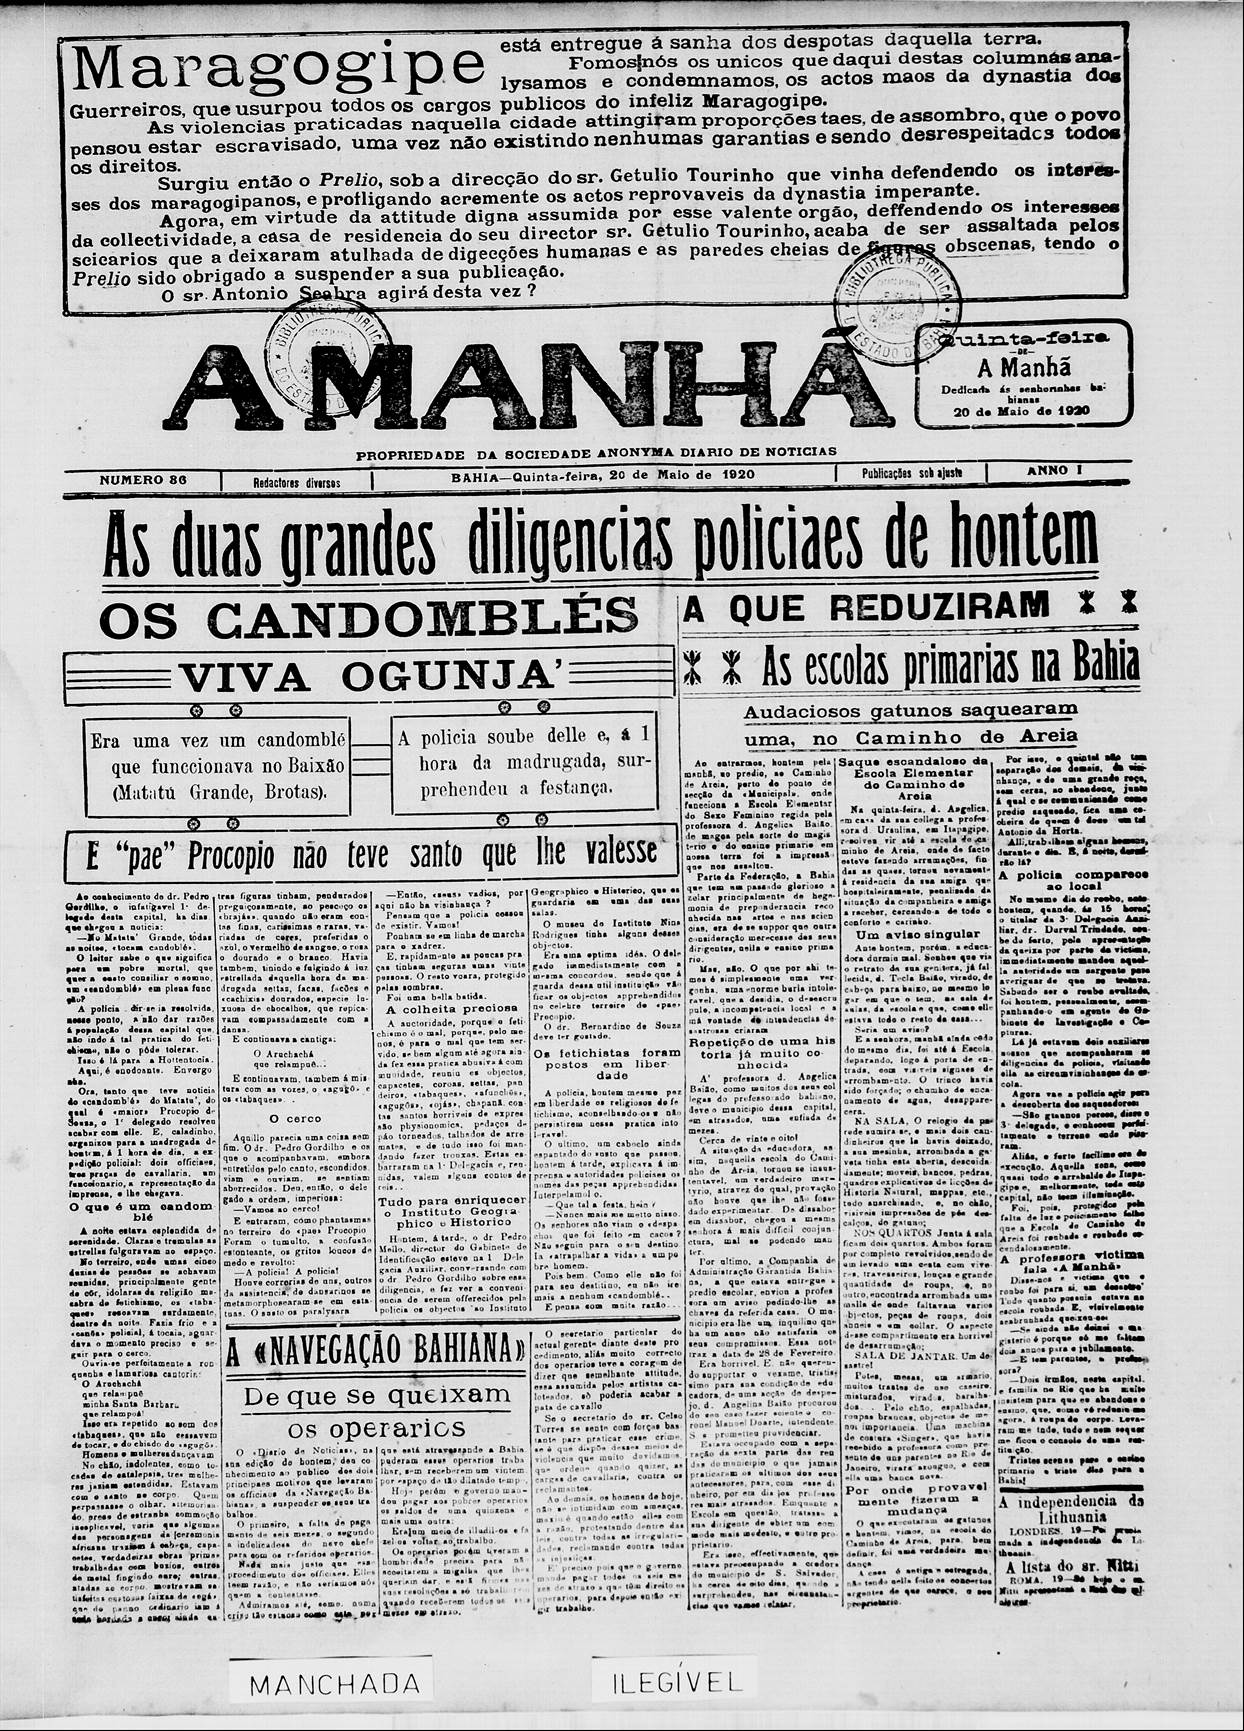
\includegraphics[width=1\textwidth]{4-cap3/complementos/imagens/19200520-vivaogunja.jpg}{\par \footnotesize \textbf{Fonte:} \textbf{A Manhã}, ano I, nº 36, 20 maio 1920, p. 1. }
\label{fig:vivaogunja}
\end{figure}

Em setembro de 1914 noticiava-se --- com as habituais solicitações de providências por parte da polícia --- a existência de duas casas do ``maldito e ruidoso candomblé'', ``uma sita à rua Uruguayana e a outra em uma ladeira por detraz do Asylo São João de Deus''\footnote{\textbf{A Notícia}, ano I, nº 4, 23 set. 1914, p. 2.}. Como visto na \autoref{subsec:pontrel} (p. \pageref{subsec:pontrel}), o terreiro \textit{Tumba Junsara}, fundado anos depois, em 1919, foi instalado na Ladeira do Pepino por volta de 1920; é certo que o terreiro da Uruguaiana a que se refere a notícia não é ele, mas é muito provável que a existência de terreiros mais antigos na Boa Vista e no Engenho Velho tenha de algum modo influenciado a escolha de sua nova localização.

Em maio de 1920 chegou ao famigerado Pedro Gordilho, delegado de polícia, a informação de que ``no Matatú Grande'', ou mais especificamente na localidade conhecida ainda hoje como Baixão, ``todas as noites `tocam candomblé' ''. Em diligência ao local em alta madrugada\footnote{A notícia indica que à 1h se cantava, ao som de atabaques e agogôs, uma cantiga assim registrada: ``O Aruchachá / que relampuê / minha Santa Bárbara / que relampoá!''; o mais provável é que se tratasse de um culto a Iansã.}, o destacamento policial comandado pelo próprio Gordilho irrompeu terreiro adentro aos gritos de ``polícia! polícia!'', prendendo vinte pessoas (que se diz terem sido postas em liberdade no dia seguinte, sabe-se lá em que condições) e pondo em fuga outras tantas. O terreiro foi assim desmantelado, todos os objetos sagrados e litúrgicos do templo --- ``capacetes, coroas, settas, pandeiros, `tabaques', `afunchês', `agugôs', `ojás', chapanã, contas, santos horriveis de expressão physiognomica, pedaços de páo talhados, talhados de arremate'' --- foram apreendidos, e tudo foi entregue ao Instituto Geográfico e Histórico da Bahia por sugestão de Pedro Melo, do Gabinete de Identificação\footnote{\textbf{A Manhã}, ano I, nº 36, 20 maio 1920, p. 1.}. Nove dias depois da matéria, considerada ``um sucesso'' pelo jornal, foi impetrado \textit{habeas corpus} em favor do pai-de-santo, ironizado pelo jornal por apelar ao Judiciário ao invés dos santos do candomblé, este ``abuso anti-hygienico''\footnote{\textbf{A Manhã}, ano I, nº 44, 29 maio 1920, p. 3.}, A manchete em letras garrafais da incomum matéria de meia página da capa do jornal não deixa dúvidas quanto à localização do terreiro: ``Viva Ogunjá!'' Não se pode concluir daí outra coisa senão de que se tratava do \textit{Ilê Ogunjá}, fundado em 1906 por \textit{Procópio Xavier de Souza} (1880-1958), sacerdote ketu conhecido também como \textit{Procópio de Ogum}. Muito provavelmente foi esta a prisão, ou uma das prisões, que deu base a uma das mais famosas alegorias da obra literária de Jorge Amado, iniciado ele próprio no candomblé como ogã de Oxossi no Ilê Ogunjá: o afrontamento de Procópio ao delegado ``Pedrito Gordo'', baseado no próprio Pedro Gordilho \cite[p.~236-242]{amado_tenda_2010}. O Ilê Ogunjá deu seu nome iorubá ao vale entre o Acupe e o Matatu, de um lado, e o Engenho Velho de Brotas, do outro --- e até os dias atuais, quando sobre ele corre uma avenida bastante movimentada, não há quem a conheça por seu nome oficial.

Nem a documentação pesquisada, nem a bibliografia consultada apontam quaisquer outras ocorrências, que para emergirem da poeira dos arquivos precisariam de outro tipo de pesquisa, de outras fontes, de outro tempo. Cabe registrar, como nota final sobre o assunto, duas coisas. 

Em primeiro lugar, os terreiros mencionados, junto ao \textit{Alaketo} ainda existente no período no Matatu, são ou foram terreiros grandes, bastante conhecidos; está ainda em curso, em especial por meio da arqueologia, a construção de uma base historiográfica acerca dos terreiros menores, domésticos, mais fáceis de se ocultar num cenário político repressivo mas ao mesmo tempo mais vulneráveis à repressão quando a sofriam, e portanto mais efêmeros \cite{gordenstein_arqueterre_2016}; no caso de Brotas, uma tal pesquisa sequer existe, tanto pela falta de uma base de dados tal como a que vem sendo construída acerca dos candomblés do século XIX \cite{reis_candomble_2001}, quanto pelo fato de que, diferentemente do que se deu no Pelourinho e adjacências, onde tais pesquisas arqueológicas e arquivísticas logram maior sucesso, o desenvolvimento urbano em Brotas resultou em sucessivas demolições e reconstruções, arrancando assim do solo significativa matéria-prima arqueológica. Uma base de dados sobre os candomblés domésticos em Brotas pode ser construída, e certamente a base de dados relativa aos candomblés baianos do século XIX a contempla; o difícil é encontrar os traços e rastros arqueológicos dos terreiros menores. Veja-se, como exemplo destes terreiros menos conhecidos em Brotas, a notícia de que em junho de 1904 uma ``força de Urbanos'' atacou um terreiro na estrada da Cruz das Almas e prendeu oito pessoas\footnote{\textbf{Correio do Brasil}, ano II, nº 231, 07 jun. 1904, p. 2}; se o \textbf{Mapeamento dos Terreiros de Salvador} (\url{http://www.terreiros.ceao.ufba.br}) foi muito útil relativamente aos terreiros maiores e mais conhecidos, no que diz respeito a terreiros já desaparecidos como este a ferramenta mostrou suas limitações, pois aquilo que hoje deve constar quiçá apenas da memória genealógica de algumas casas não fica nele registrado, e este terreiro da estrada da Cruz das Almas não aparece em mais referência alguma. 

Em segundo lugar, não se pode deixar de registrar como a aguerrida resistência dos praticantes do candomblé em Brotas produziu um curioso efeito. Os mais conhecidos pontos notáveis de Brotas na atualidade não são, como na Primeira República, as igrejas e as grandes herdades, palacetes e mansões; são as \textit{avenidas de vale}, cuja importância transcende o território do distrito. Ora, duas das mais importantes delas, a Bonocô (Mário Leal Ferreira) e a Ogunjá (General Graça Lessa), devem seu nome mais conhecido não a uma ``origem popular'' de memória perdida, mas sim a dois terreiros de candomblé muito antigos. 

\subsection{Eventos cívico-políticos}

Prosseguiam as comemorações do Dois de Julho no distrito tão animadas --- ou mesmo mais, quem sabe! --- quanto nos tempos imperiais:

\begin{citacao}
\textbf{2 de Julho do Castro Neves}

Da comissão organisadora desses festejos, recebemos um delicado convite a que agradecemos, para assistirmos ao desfilar do prestito que se realizará no proximo domingo, 6 do corrente, a 1 hora da tarde, sahindo do Largo da Boa Vista e seguindo pelas ruas 1º de Março, Pitangueiras, Largo do Paranhos, Matatú Pequeno, Fabricio, Sangradouro, Sete Portas, regressando pela Ladeira do Santo Agostinho, rua da Alegria, Socorro, Ladeira dos Galés, Fonte Nova, donde se dirigirá para o Castro Neves, que estará festivamente embandeirado.

Ao passar pelo Matatu pequeno falará o acadêmico Lemos Britto.

Os festejos prolongar-se-ão até o dia 8.

O programma é o seguinte!

Abrira a comitiva civica um grupo numeroso de cavalheiros, trajados symbolicamente;

seguir-se-á uma banda de clarins, fanfarreando em toques estridentes, e annunciando à multidão anciosa a aproximação do imponente e magestoso prestito;

segue-se um piquete de cavallaria;

virá depois um pelotão de cornetas e caixas de guerra, surgindo então, da immensa massa do povo, o Carro Emblematico;

musica de S. Vicente de Paulo;

batalhão de graciosas meninas symbolisando as \og Heroinas Brasileiras \fg{};

banda do 2º corpo do Regimento Policial;

batalhão de meninos \og Defensores do Castro Neves \fg{};

musica dos Salesianos, seguindo-se o collegio encorporado da referida associação beneficente;

banda do 1º corpo policial;

banda do 5º batalhão de artilharia, etc., etc.\footnote{\textbf{Correio do Brazil}, ano III, nº 567, 4 ago. 1905, p. 4}
\end{citacao}

Os festejos bijulinos eram ainda realizados no Castro Neves em 1914\footnote{\textbf{Gazeta de Notícias}, ano IV, nº 230, 01 jul. 1914, p. 1.}, e em 1915 ocorriam também na vizinhança da Capela do Deus Menino\footnote{\textbf{A Notícia}, ano I, nº 260, 05 ago. 1915, p. 1.}.

As celebrações particulares também eram dignas de nota, em especial quando ligadas a políticos. Frederico Costa, presidente do Senado estadual, enraizava seu poder político nas terras de sua propriedade ao Matatu, onde tinha uma fazenda produtora de laranjas e vários imóveis urbanos; num seu aniversário, em 1927, um jornal notoriamente seabrista esculhambou-o de cima a baixo, chamando-o de ``homúnculo [\dots] [\textit{que}] de discursos [\dots] pouco entende'', ``rubicundo politiqueiro [\dots] cuja obtusidade é compacta, é integral, é profunda'' --- e entre um impropério e outro, registrou que naquela data, em seguida a uma missa na Sé, o Matatu amanhecia ``embandeirado em arco'' pela festa de aniversário do político, ``com gyrandolas, comidas e bebidas''\footnote{\textbf{O Combate}, ano I, nº 120, 29 out. 1927, p. 1. O mesmo jornal prosseguiu na catilinária contra Frederico Costa em várias edições posteriores.}.

\subsection{Eventos religiosos, festivos e carnaval}

O calendário de festas religiosas católicas soteropolitanas celebradas também no distrito de Brotas incluia o \textit{Natal}, celebrado em 1914 no ``aprazível arrabalde'' da Pituba com ``muitas diversões que se prolongarão até ao romper do dia, com o espoucar de foguetes, tocando um grupo musical, havendo kermesse e outras surpresas''; na Boa Vista estava programada a apresentação de um coral infantil, da banda do Corpo de Bombeiros e uma procissão infantil carregando a imagem do ``menino Deus'' (seria a mesma da Capela do Deus Menino, bastante próxima?); no ``lindo trecho'' da Alagoa seria realizada uma missa\footnote{\textbf{A Notícia}, ano I, nº 83, 24 dez. 1914, p. 7.}. Quanto a esta última, a tradição pode ter sido iniciada em 1898, ano em que ``um grupo de rapazes e moças passeiantes, moradores na Fonte do Boi e nas Pedrinhas'', foi pedir permissão ao ``coronel Juca Amaral'' para celebarar na capela de Nossa Senhora dos Mares da Lagoa uma missa natalina\footnote{\textbf{Jornal de Notícias}, ano , nº , 13 dez. 1898, p. 2.}.

Outra celebração por meio da qual Brotas se inseria no calendário de festas religiosas soteropolitanas era a \textit{queima do Judas}, como se deu no Sangradouro em 1905 \footnote{\textbf{Correio do Brasil}, ano III, nº 486, 24 maio 1905, p. 2.}. Comemorava-se também em Brotas a \textit{folia de Reis}: em 1914, além da saída do terno \textit{Concha de Ouro} da Alegria do Castro Neves\footnote{\textbf{Gazeta de Notícias}, ano IV, nº 94, 03 jan. 1914, p. 1.}, foi anunciado que no Rio Vermelho ``funccionarão, durante toda a noite, o \textit{roskoff} e a \textit{kermesse}, devendo alli comparecer os ranchos do \textit{Saramonete}, que sahirá do Grão-Mogol, e o do \textit{Bebê}, que sahirá do arrabalde de Amaralina''\footnote{\textbf{Gazeta de Notícias}, ano, nº , 5 jan. 1914}; no caso de Amaralina, é muito provável que participasse de algum modo na organização dos festejos o \textit{Centro Recreativo de Amaralina}, do qual era vice-presidente em dezembro de 1913 o jovem Alberto Magalhães\footnote{\textbf{Gazeta de Notícias}, ano IV, nº 71, 04 dez. 1913, p. 2.}.

Os ranchos, entretanto, eram vistos na época como ``elemento de desordem'': o \textit{Curuvina}, por exemplo, sediado no Dique Pequeno, foi destacado pela imprensa por causa de uma briga ocorrida numa de suas noites de ensaio, ``onde a \textit{pura} é o estimulante procurado para as libações do \textit{pessoal}''; postas as coisas em tom francamente moralista, perguntava-se o articulista, sarcasticamente, se ``a \textit{Curuvina} ainda virá á tona''\footnote{\textbf{A Notícia}, ano I, nº 42, 06 nov. 1914, p. 5.} --- ou seja, se a continuidade de seus ensaios seria permitida pelas autoridades. Como se vê, os ranchos dos bons moços de Amaralina e do Grão-Mogol eram tratados de forma muito diversa dos ranchos dos proletários, muito provavelmente negros, do Dique Pequeno.

Muito própria do distrito era a \textit{festa de Nossa Senhora da Luz}, assim anunciada em 1905:

\begin{citacao}
No proximo domingo realisar-se-à com toda a pompa a festa de N. S. da Luz, na Pituba, promovida por famílias que se acham veraneando no salubre e pitoresco arrabalde da Pituba.

Ás 5 horas da madrugada serão annunciadas as festas por 21 tiros, às 8 horas da manhã será realizada a missa e às 11 horas terá começo a festa religiosa, sendo pregador o Monsenhor Novaes.

Às 3 horas da tarde sahirá em procissão a imagem de N. Senhora, carregada por distinctas senhoras e tendo a frente a banda de música do Regimento Policial. A noite tocarà em um palanque uma musica, havendo leilão, kermesse e finalisando a festa com um bonito fogo de artifício.

Na segunda-feira haverá corrida de jangadas e outros divertimentos, terminando os festejos na terça-feira por passeiatas populares\footnote{\textbf{Correio do Brasil}, ano III, nº 420, 10 fev. 1905, p. 1.}.
\end{citacao}

O carnaval era também comemorado em Brotas durante a Primeira República, como se vê no anúncio de que em 1919 percorria a Estrada 2 de Julho na segunda e na terça de carnaval o cordão \textit{A Censura}\footnote{\textbf{A Hora}, ano II, nº 44, 01 mar. 1919, p. 3.}.